\RequirePackage{cmap}%kopieren aus dem pdf
\documentclass[a4paper,12pt]{report}
\usepackage[paper=a4paper,top=30mm,bottom=30mm]{geometry}%,twoside

%\usepackage{a4wide}
%\usepackage{ngerman}
\usepackage[ngerman]{babel}
\selectlanguage{ngerman}

\usepackage[utf8]{inputenc}

\usepackage[T1]{fontenc}% die beidne sachen fürs aus dem pdf kopieren
\usepackage{lmodern}% schaden aber auch so nix glaub ich (lmodern provoziert eine vektorschrift imho)

\usepackage{amsfonts}
\usepackage{amsmath}
\usepackage{amsthm}
\usepackage{amssymb}
%\usepackage{float} %
%\usepackage{yfonts}
\usepackage{xspace}
\usepackage{fancybox}
\usepackage{graphicx}
\usepackage{floatflt}
\usepackage{url}
\usepackage{listings}
\usepackage{boxedminipage}
\usepackage{float}
\usepackage{sepnum}
\usepackage{placeins}
\usepackage{rotating}
\usepackage{threeparttable}
\usepackage[multidot]{grffile}
\usepackage{epigraph}
\usepackage[normalem]{ulem}
\usepackage[comma,authoryear]{natbib}
\usepackage[pdfborder={0 0 0}]{hyperref} %hyperref funktioniert leider nicht mit dvips, mit pdflatex aber schon
\usepackage{hypernat}%damit hyperref und natbib besser harmonieren (funktioniert aber immer noch nicht :-( )
%\hypersetup{colorlinks=false}
\usepackage{microtype}
\usepackage{caption}
\usepackage{dcolumn}
\captionsetup{justification=justified}
\usepackage{booktabs}
%\usepackage{color}
\usepackage{subfig}
\usepackage{xyling}%Bäume, wichtig: wenn mit pdflatex benutzt, muss in der datei xyling.sty die Zeile "`\RequirePackage[color,all,dvips]{xy}"' zu "`\RequirePackage[color,all]{xy}"` geändert werden
%\usepackage[all]{hypcap} %damit auf den anfang eines bildes verwiesen wird (macht angeblich sonst probleme, siehe http://en.wikibooks.org/wiki/LaTeX/Labels_and_Cross-referencing)
%\usepackage{lmodern}%bringt nix %Standardschriftart, damit hoffentlich das aus dem pdf kopieren von umlauten funktioniert
%\usepackage{MnSymbol}

\begin{document}
\allowdisplaybreaks%Mathe darf auch umbrechen
\newcommand{\todo}[1]{\begin{Huge}\emph{[ToDo: #1]}\end{Huge}}
%\newcommand{\f}[0]{\textnormal{f}}
\newcommand{\datum}[3]{#3.\,#2.\,#1}%Tag Monat Jahr gesetzt nach DIN ... #1 - year #2 - month #3 - day
\newcommand{\func}[1]{\textnormal{#1}}
\newcommand{\code}[1]{\textnormal{#1}}
\newcommand{\stichprobentabelleninneres}[1]{\texttt{#1}}
\newenvironment{bsp}{\subparagraph{Beispiel}}{~\\}
\newenvironment{bem}{\subparagraph{Anmerkung}}{~\\}
\newenvironment{rahmen}{\begin{boxedminipage}{\linewidth}}{\end{boxedminipage}}
\newenvironment{webseitenausschnitt}{\paragraph{}\begin{rahmen}}{\end{rahmen}\paragraph{}}
\newcommand{\dotcup}{\ensuremath{\mathaccent\cdot\cup}}
\newcommand{\setN}{\mathbb{N}}
\newcommand{\setR}{\mathbb{R}}
\newcommand{\pow}[1]{2^#1}
\newcommand{\average}{\varnothing}
\newcommand{\property}[1]{\url{#1}}
\newcommand{\article}[1]{\url{#1}}
\newcommand{\prefix}[1]{\url{#1}}
\newcommand{\definition}[1]{\textit{#1}}
\newcommand{\val}[1]{\sepnum{,}{\,}{}{#1}}
\newcommand{\valunit}[2]{\val{#1}\,#2}
\newcommand{\valrange}[2]{\val{#1} -- \val{#2}}
\newcommand{\valunitrange}[3]{\val{#1} -- \valunit{#2}{#3}}
% Functions
%\newcommand{\T}{\textnormal{T}}
\newcommand{\s}{\textnormal{s}}
\newcommand{\f}{\textnormal{f}}
\newcommand{\g}{\textnormal{g}}
\newcommand{\h}{\textnormal{h}}
%Theorems
\theoremstyle{remark}
\newtheorem{rem}{Bemerkung}
\theoremstyle{definition}
\newtheorem{dfn}{Definition}
%Abbreviations
\newcommand{\zb}{\mbox{z.\,B.}\xspace}
%\newcommand{\figref}[1]{Abbildung \ref{fig:#1}}

\long\def\symbolfootnote[#1]#2{\begingroup%
\def\thefootnote{\fnsymbol{footnote}}\footnote[#1]{#2}\endgroup} 
\lstset{language=Java}
\lstset{flexiblecolumns=true}

%\topmargin-5.4mm %default 25.4mm
%\topmargin-20mm
\tableofcontents

\chapter*{Einleitung}
\addcontentsline{toc}{chapter}{Einleitung}%damit es auch ohne Nummer im Inhaltsverzeichnis auftaucht

Seit Jahrzehnten besteht die Vision eines sprechenden Computers -- zunächst nur als Gegenstand kühner Science Fiction, später jedoch als ernsthafte Motivation der Computerlinguistik,
deren Forschungsgebiet die Entwicklung von Algorithmen zur Verarbeitung menschlicher Sprache ist. 
Während das ultimative Ziel menschengleichen Sprachverständnisses schon aufgrund gänzlich unterschiedlicher Erfahrungswelten trotz intensiver Forschung noch unerreichbar scheint, sind bereits beeindruckende
Fortschritte bei der Extraktion von Informationen aus geschriebener Sprache -- dem Textmining -- erreicht worden.
Gleichzeitig wurden aber auch Erfahrungen über die prinzipiellen Hindernisse gesammelt, die einem umfassenden Verständnis entgegenstehen.
So ist das Verständnis einer Grammatik nur ein kleiner Teil zum Verstehen eines Satzes, welches selbst in sehr einfachen Fällen ein großes Maß an Weltwissen voraussetzt.
Dieses liegt jedoch nicht in einer für Maschinen verarbeitbaren Form vor.

Die Einführung des \emph{Semantischen Webs} bringt dazu eine Gegenströmung, deren Ziel nicht das Beherrschen der komplexen natürlichen Sprachen durch Computer ist,
 sondern der Aufbau eines gigantischen Netzes von Agenten und Wissensbasen, die durch die simple, formale, jedoch nicht zweckgebundene Sprache \emph{RDF} miteinander kommunizieren und damit vielfältige Aufgaben erledigen können.
Weiterhin werden Schnittstellen entwickelt, die es dem Menschen so einfach wie möglich machen sollen, ihre Anfragen in dieser Sprache auszudrücken.
Da es jedoch sehr aufwändig sein kann, bestehende natürlichsprachige Wissensquellen manuell in das Format des Semantischen Webs zu konvertieren,
 ist dieses auf effiziente Methoden der natürlichen Sprachverarbeitung angewiesen, um bereits existierende Information aufzunehmen.

Ziel dieser Arbeit ist es, ein Framework namens \emph{NLP2RDF} zu entwickeln, das eine Brücke zwischen natürlicher Sprachverarbeitung und dem Semantischen Web -- zwischen Syntax und Semantik -- schlägt.
NLP2RDF enthält eine Pipline, die viele verschiedene Tools zur Verarbeitung natürlicher Sprache und Wissensquellen des Semantischen Webs integriert 
und mithilfe dieser Tools aus geschriebenen Sätzen eine RDF-Struktur erstellt, welche explizit die implizite Bedeutung dieser Sätze ausdrückt.
Zusätzlich zu Adaptern zu bereits bestehenden Anwendungen wurde ein Mapping namens \emph{Wortschatz2DBpedia} zwischen den statistischen Informationen des \emph{Projektes Deutscher Wortschatz} \citep{wortschatz} und dem semantischen Weltwissen aus \emph{DBpedia} \citep{dbpedia} erstellt und eine
Wortsinndisambiguierung entwickelt.
Weiterhin setzt NLP2RDF mit dem \emph{DL-Learner} \citep{dl-learner} Algorithmen des maschinellen Lernens ein, um aufgrund des generierten Hintergrundwissens Text zu klassifizieren.
Damit lassen sich sowohl syntaktische ("`es handelt sich um einen Passivsatz"'), als auch semantische Features ("`der Text enthält Referenzen auf einen Politiker der Gegenwart"') bestimmen.
Dieser Ansatz stellte sich schnell als so vielversprechend heraus, dass das Projekt mit Herrn Sebastian Hellmann im Rahmen seiner Dissertation \citep{nlp2rdf_hellmann_thesis} parallelentwickelt wird, um das volle Potential auszuschöpfen.
In Folge dessen konzentriert sich diese Arbeit auf das Mappingmodul \emph{Wortschatz2DBpedia} und die Wortsinndisambiguierung.

% Die Arbeit ist folgendermaßen aufgebaut: Im ersten Kapitel werden die Grundlagen beschrieben, die für das Verständnis der Arbeit notwendig sind.
% Im zweiten Kapitel wird der Aufbau von NLP2RDF erklärt.
% Das Mapping Wortschatz ... Kapitel ..


%... nlp2rdf hilft beiden es nimmt sachen vom semantic web um nlp zu helfen (disambiguierung und so) und es nimmt sachen von nlp (parser wortschatz ,...) um dem wortschatz zu helfen

\iffalse
Die Klassifikation von geschriebenem Text ist ein Problem mit einem sehr vielfältigen Einsatzgebiet.
E-Mail-Programme teilen eingehende Post in \emph{erwünschte} und \emph{nicht erwünschte} Nachrichten auf.
Suchanfragen müssen zwischen \emph{relevanten} und \emph{nicht relevanten} Webseiten unterscheiden.
Diktatorische Staaten versuchen, \emph{regimekritische} Botschaften zu unterdrücken.
Literaten wollen herausfinden, ob ein lang verschollenes Buch von Shakespeare geschrieben wurde.
Lehrer suchen Beispielsätze einer bestimmten Struktur, zum Beispiel \emph{Aktiv- und Passiv-}, \emph{Konditional-}, \emph{besonders lange}, \emph{besonders kurze} oder \emph{für eine bestimmte Zeit typische} Sätze.
Herausgeber möchten zwischen \emph{lustigen} und \emph{nicht lustigen} Witzen, \emph{leckeren} und \emph{weniger leckeren} Kochrezepten,
\emph{gesellschaftlich akzepterten} und \emph{nicht akzeptierten} Büchern differenzieren.
Ein Freund der Kälte möchte seine Texte nach der gefühlt dort beschriebenen Temperatur sortieren.
Studenten würden gerne zwischen einer \emph{gerade so abgabefähigen}, \emph{normalen}, \emph{herausragenden} Diplomarbeit und \emph{einer, die sie sofort um die Ohren geschlagen bekommen} unterscheiden können.

Das einzige was all diese Anforderungen eint, ist dass sie komplett voneinander verschieden sind.
Schon bei der blossen Betrachtung wird einem klar, dass man keineswegs alle Probleme der Textklassifikation wird lösen können.\footnote{"`Beschreibt dieser Text eine Turingmaschine, die hält?"', wäre so ein
Problem der schwereren Kategorie.}
Diese Arbeit beschränkt sich daher auf ein, jedoch immer noch sehr umfangreiches, Teilproblem.

Im Kern des entwickelten Programmes steht ein Adapter zu einem Parser, der die Phrasenstruktur des eingegebenen Textes erkennt. Diese Struktur wird dann in RDF modelliert und wie ein Weihnachtsbaum 
von beliebigen weiteren Tools mit Zusatzinformationen behängt.

Mit entwickelt wurde dabei ein Tool namens \emph{Wortschatz2DBpedia}, welches über die maschinenverarbeitbaren Daten des DBpedia-Projekts die Brücke zum Weltwissen der Wikipedia schlägt.
Aufgrund der offenen Struktur des Programmes ist es jedoch möglich und erwünscht, dass weitere Adapter zu anderen Tools hinzugefügt werden um das Einsatzgebiet zu erweitern.
Um dies zu ermutigen, wurde es strukturiert programmiert, unter einer Open Source-Lizenz bei Google Code gehostet, gut kommentiert und im Rahmen dieser Arbeit auch dokumentiert
(Details und Programmierbeispiele finden sich vor allem im Anhang).


Diese Diplomarbeit beschränkt sich daher auf folgendes Teilproblem:
\begin{itemize}
\item gegeben sei eine Menge von positiven (P) und negativen (N) Beispielen, wobei nur P nicht leer sein darf
\item die Sprache des Textes ist englisch oder deutsch
\item Es gibt keine verschiedenen, sich überlappenden Kategorien. Entweder ein Text gehört der Menge X an, oder eben nicht.
\item es existiert eine ausgezeichnete Trainingsmenge, bestehend aus positiven und eventuell auch negativen Beispielen
\item die Zugehörigkeit zur Menge X lässt anhand von einfachen Definitionen, die in OWL formuliert sind, beschreiben
\item die Gemeinsamkeit beruht entweder auf der Satzstruktur, oder lässt sich aus dem Weltwissen, das in der Wikipedia enthalten ist, schlussfolgern
\end{itemize}


%Es muss also ein all
%Linguisten möchten alle Sätze aufspüren, die ein bestimmtes Sprachfeature aufweisen, Herausfinden, was die Gemeinsamkeit einer bestimmten Menge von Texten ist und 

Ein modulares erweiterbares Programm wurde entwickelt, welches Tools der Sprachverarbeitung mit Methoden des Semantischen 
Einsatzzweck ist die Klassifikation von Text jeder Art.

Textklassifizierungsaufgaben jedweder Art können damit 
%auf der einen Seite mit der LOD-Cloud des Semantic Web verbindet.
Adaptoren für diese Tools sind also das Herzstück des Programmes. Je nach Einsatzzweck werden aus diesen Adaptoren dann diejenigen aktiviert, die als nötig erachtet werden.


Kernstück des Programmes ist Adaptoren für diese Tools. 
\fi

% Einleitung von Christian Biemann:
\iffalse
In den nunmehr über 60 Jahren, die seit der Erfindung der elektronischen
Rechenmaschine vergangen sind, wurde die Welt durch die Möglichkeit,
immer      schneller    und   preiswerter  immer   größere   Berechnungen
durchzuführen, nachhaltig verändert. Schon früh kamen in der Science-
Fiction-Literatur sprechende Computer vor – Automaten, die verstehen,
was ein Mensch oder ein anderes künstliches Wesen ihnen mittels
natürlicher Sprache mitteilt, und die ihrerseits darauf in einer Weise
antworten, als hätten sie begriffen, worum es ging. Der Mythos des
allwissenden und alles könnenden Computers beherrscht nach wie vor die
Köpfe der Menschen, auch wenn die Vision eines elektronischen
Gesprächspartners immer noch wie Zukunftsmusik klingt.
Weil Berechnungen in Schritten erfolgen, muß der menschliche Geist
zunächst alle Schritte der Berechnung verstanden haben, bevor er sie in
eine Maschine implementieren kann. Dabei hat sich die Implementierung
von menschlicher Sprache, dem Charakteristikum des Menschen, in dem
er sich von allen anderen Lebewesen auf dieser Erde unterscheidet, als
besonders schwierig erwiesen. Vorliegende Arbeit soll auf dem Weg
dorthin ihren bescheidenen Beitrag leisten.
Ziel der Arbeit war es, semantische Relationen zu erlernen, um diese in
natürlichsprachlichen Texten erkennen zu können. Es wurde ein
Verfahren entwickelt, das mit Hilfe einer großen Textsammlung Wörter
lernt, die in einer bestimmten Relation zu anderen Wörtern stehen. Hierbei
soll sich durch ein kleines vorausgesetztes Grundwissen hoher Datenertrag
ernten lassen.
Die Arbeit ist folgendermaßen aufgebaut: Im ersten Kapitel wird eine
Einordnung der Arbeit in die beteiligten wissenschaftlichen Gebiete
                     Es   folgt   eine   Übersicht über   die  verwendete
vorgenommen.
                                       -3-
-
Textsammlung, sowie über verschiedene semantische Relationen, und wie
diese beschaffen sein müssen, damit sie für das Verfahren geeignet sind.
Im zweiten Kapitel wird der dem Verfahren zugrundeliegende
Algorithmus erklärt. Nach einigen Vorüberlegungen zur theoretischen
Beschaffenheit der gesuchten Relationen wird der Algorithmus im Detail
dargelegt. Es folgen Betrachtungen zum erwarteten Verhalten, sowie zu
Voraussetzungen, die für den Erfolg des Verfahrens notwendig sind.
Die durch eine Implementierung des Verfahrens erzielten Ergebnisse
werden in Kapitel drei vorgestellt. Hauptgegenstand der Untersuchungen
war die semantische Relation, die zwischen Vor- und Nachnamen besteht.
Das Verhalten der Implementierung wurde aber auch an anderen
Relationen untersucht. Das vierte Kapitel enthält Ausblicke zu weiteren
Relationen, außerdem werden Verbesserungen und andere Anwendungs-
gebiete diskutiert. Eine Anwendung des Verfahrens in leicht modifizierter
Form findet sich im fünften Kapitel. Ziel dieser Anwendung war es,
Personennamen in Texten zu markieren und die Berufe der Personen der
aktuellen Zeit zu finden. Im sechsten Kapitel finden sich abschließende
Bemerkungen.
\fi
\iffalse
\subsection{Ziele}
Ziel ist es, beliebige Sprachfeatures mit Hilfe vorgegebener Texte zu erlernen.
Dabei sollen anhand von positiven und negativen Beispielen Regeln in einer Beschreibungslogik aufgestellt werden.
Dazu soll ein Programm geschaffen werden, welches ein Adapter für bereits existierende Tools zum Aufbereiten von Text ist.
Ein Chunker, ein Parser und eine Verbindung zu DBpedia sollten dabei enthalten sein, jedoch mit der Möglichkeit, jederzeit neue Teile hinzuzufügen.
Eingegebener Text wird dabei erst in eine einfache RDF-Struktur umgewandelt und dann beliebig mit Informationen aus den gewählten Tools erweitert.
Der DL-Learner, ein Programm, welches Konzepte in Beschreibungslogiken lernt, erzeugt dann unter Eingabe dieser RDF-Strukturen die gesuchten Regeln.
\fi
\chapter{Grundlagen}\label{sec:grundlagen}
Die für das Verständnis dieser Arbeit notwendigen Fachbegriffe und sind hier aufgeführt.
\section{Konventionen}
\begin{table}[ht]
\begin{tabular}{ll}
\toprule
Präfix	&URL\\
\midrule
nlp2rdf		&http://nlp2rdf.org/ontology/\\
en-wiki		&http://en.wikipedia.org/wiki/\\
dbpedia		&http://dbpedia.org/resource/\\
dbpedia-owl	&http://dbpedia.org/ontology/\\
dpprop		&http://dbpedia.org/property/\\
foaf		&http://xmlns.com/foaf/0.1/\\
owl		&http://www.w3.org/2002/07/owl\#\\
rdf		&http://www.w3.org/1999/02/22-rdf-syntax-ns\#\\
skos		&http://www.w3.org/2004/02/skos/core\#\\
yago		&http://dbpedia.org/class/yago/\\
\bottomrule
\end{tabular}
\caption{Namensraum-Präfixe}
\label{tab:namespace-prefixes}
\end{table}

\begin{table}[ht]
\begin{tabular}{ll}
\toprule
%\midrule
$\propto$	&Proportional zu\\
$\average$	&Durchschnitt (Arithmetisches Mittel)\\
$2^M$		&Potenzmenge\\
\bottomrule
\end{tabular}
\caption{Mathematische Symbole}
\label{tab:}
\end{table}

% \begin{table*}[ht]
% \begin{tabular}{ll}
% \toprule
% Betonung,\\
% neu eingeführter Begriff 	&\emph{Projekt Deutscher Wortschatz}\\
% URL				&\url{http://code.google.com/p/nlp2rdf/}\\
% Quelltext			&
% \begin{lstlisting}[mathescape=true,texcl,language=java,escapechar=?]
%   public static void main(String[] args) {}
% \end{lstlisting}\\
% \bottomrule
% \end{tabular}
% \caption{Schriftsatzkonventionen}
% \label{tab:}
% \end{table*}
Sämtliche numerischen Werte sind, sofern nicht anders angegeben, auf vier Nachkommastellen kaufmännisch gerundet nach \emph{DIN 1333}.
\iffalse Sie sind nicht alphabetisch, sondern logisch geordnet und bauen aufeinander auf.
Ein von-oben-Lesender kann also erst das Grundlagenkapitel lesen und dann zu [insert wie auch immer der nächste teil dann heißt] übergehen.
Gleichfalls ist es möglich, mit [insert das kapitel hier] zu beginnen, und bei Unklarheiten hier nachzuschlagen.
\fi
\FloatBarrier
\section{Das Semantische Web}
Das Ziel des \emph{Semantischen Webs} ist, dass Computeragenten Informationen verstehen können.
Diese Informationen sind durch Daten repräsentiert, die ein Netz bilden, das \emph{Web of Data}.
Dadurch können Agenten auf einfache Art und Weise Aufgaben lösen, die mit herkömmlichen Mitteln sehr aufwendig sind.

%Das WWW besteht aus untereinander verknüpften Hypertextdokumenten, welche sich der Benutzer mit einem Webbrowser anzeigen lassen kann.
% Jedes dieser Dokumente ist durch eine eindeutige \emph{URL} (Uniform Resource Locator) identifiziert.
% Der Siegeszug des WWW hat jedoch im Laufe der Jahre eine derart gigantische Informationsfülle hinterlassen, dass diese für den Menschen kaum noch erfassbar ist.
% So vermeldete Google bereits im Sommer 2008, dass sein Suchindex nun eine Billion einzigartige URLs enhielt\cite{www-google-one-trillion-urls}.
% Eine so große Menge an Webseiten ist nur noch mit Hilfe von Suchmaschinen recherchierbar.
% Diese stehen jedoch vor dem Problem, dass für sie das WWW nur aus Textbausteinen mit Verweisen besteht, weder der Text noch die Verweise enthalten jedoch normalerweise eine für 
% ein Programm verwertbare Bedeutung. Somit sind die einzig möglichen Anfragen jene nach allen Seiten, die bestimmte Wörter oder Textteile enthalten.
% Oft weiss man jedoch gar nicht, wie dass, was man sucht, heißt oder möchte eine ganz andere Art von Anfrage stellen.
Würde ein Benutzer etwa eine Auflistung aller bekannten Getränke suchen, so würde eine Suche bei einer Suchmaschine wie Google nach "`Getränk"', nur die Webseiten zurückliefern, 
welche tatsächlich das Wort "`Getränk"' enthalten.
Einen Artikel, welcher Coca Cola beschreibt, würde die Suchmaschine jedoch nicht finden, falls er das Wort "`Getränk"' in einer anderen Sprache oder gar nicht enthalten würde.
Der Suchmaschine fehlt also sowohl die Information, dass die Wörter "`Coca Cola"' und "`Getränk"' Konzepte aus der realen Welt beschreiben, als auch jene,
dass "`Coca Cola"' eine Art "`Getränk"' ist. Für dieses Problem existieren zwar Techniken wie \emph{Query expansion} und \emph{Latent Semantic Analysis},
bei komplizierteren Anfragen ("`finde alle Getränke, die keinen Zucker enthalten"') stoßen sie jedoch an ihre Grenzen. 
Ein Netz, welches für Softwareagenten geeignet ist, sollte aus Ressourcen bestehen, welche bestimmte Konzepte oder Objekte verkörpern.
Weiterhin sollte es Informationen über die Relationen dieser Ressourcen untereinander enthalten.

Die mannigfaltigen Möglichkeiten eines solchen Netzes gehen jedoch weit über die Nutzung als Recherchehilfe hinaus und haben
das Potential, ebenso revolutionäre Auswirkungen zu haben wie das World Wide Web.%\cite{lod}

%A functioning Semantic Web is predicated on the availability of large amounts
%of data as RDF; not in isolated islands but as a Web of interlinked datasets. 

Ebenso wie das WWW in seinem Anfangsstadium befindet sich das Semantic Web jedoch noch in einem Teufelskreis aus niedrigem Angebot und niedriger Nachfrage.
Solange nicht genügend Anwendungen existieren, lohnt es sich nicht, Linked Data zu erstellen und solange nicht genügend Linked Data existiert, lohnt es sich nicht, Anwendungen zu entwickeln.
Seitdem das Semantische Web in \citet{www-semantic-web-proposal} beschrieben wurde, hat sich jedoch schon einiges getan.
Damit nicht große Datenmengen als isolierte Inseln sondern als ein Netz stark untereinander verlinkter Wissensquellen vorliegen, wurde das Projekt \emph{Linking Open Data} ins Leben gerufen.
Weiterhin setzen bereits einige namhafte Firmen wie BBC Semantic-Web-Technologien ein, um automatisch relevante Zusatzinformationen zu ihren Artikeln anzuzeigen \citep{bbc}.
%der wert von einem knoten (oder link?) im netz steigt mit der anzahl der knoten/links die drin sind -> cite irgendwas mit netzeffekten
%das web stieg auch erst ganz langsam an und explodierte (exponentiell?) dann irgendwann
%es ist nichtmehr ganz so schlimm wie am anfang 
%so setzen viele firmen wie bbc das ein um daten zu ihren artikeln zu generieren -> siehe bbc paper
%Ausführlich beschrieben sind Einige davon in einem Artikel von Tim Berners-Lee, dem Direktor des W3C (World Wide Web Consortium).\cite{www-semantic-web-proposal}
%Das Semantische Web wurde zuerst 2001 in einem Artikel von Tim Berners-Lee et al. \cite{www-semantic-web-proposal} beschrieben und wird durch eine Menge von Techniken realisiert, die auf dem WWW (World Wide Web) aufbauen.
Realisiert wird das Semantische Web durch eine Menge von Techniken, die auf dem WWW aufbauen.
\subsection{Uniform Resource Identifiers}
Eine \emph{Uniform Resource Identifier (URI)} (engl. "`einheitlicher Bezeichner für Ressourcen"') ist eine Zeichenfolge zur Identifizierung einer abstrakten oder physikalischen Ressource \citep{www-uri}.
URIs können zur Identifizierung beliebiger Konzepte verwendet werden, zum Beispiel von Webseiten, Dateien, 
Datenbankeinträgen, Personen, Gegenständen, Zahlen oder Zeichenketten.

% \begin{figure}[htb]
% \begin{threeparttable}
% 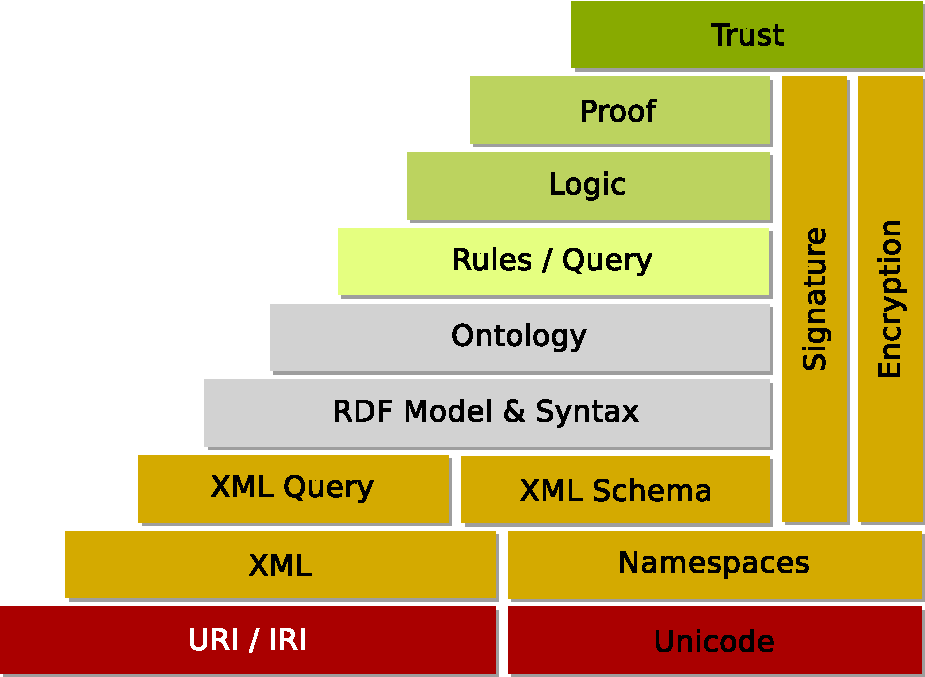
\includegraphics[width=0.6\textwidth]{img/pdf/w3c-semantic-web-layers.pdf}
% \begin{tablenotes}
% \item [1] In Zeile i: Die Differenz des Ähnlichkeitswertes zwischen Zeile i und Zeile i+1
% \end{tablenotes}
% \end{threeparttable}
% \caption[]{Die Komponenten des \emph{Semantic Web Stacks}}}
% \label{fig:semantic-web-stack}
% \end{figure}

\begin{figure}[htb]
    \begin{threeparttable}
    \centering  
    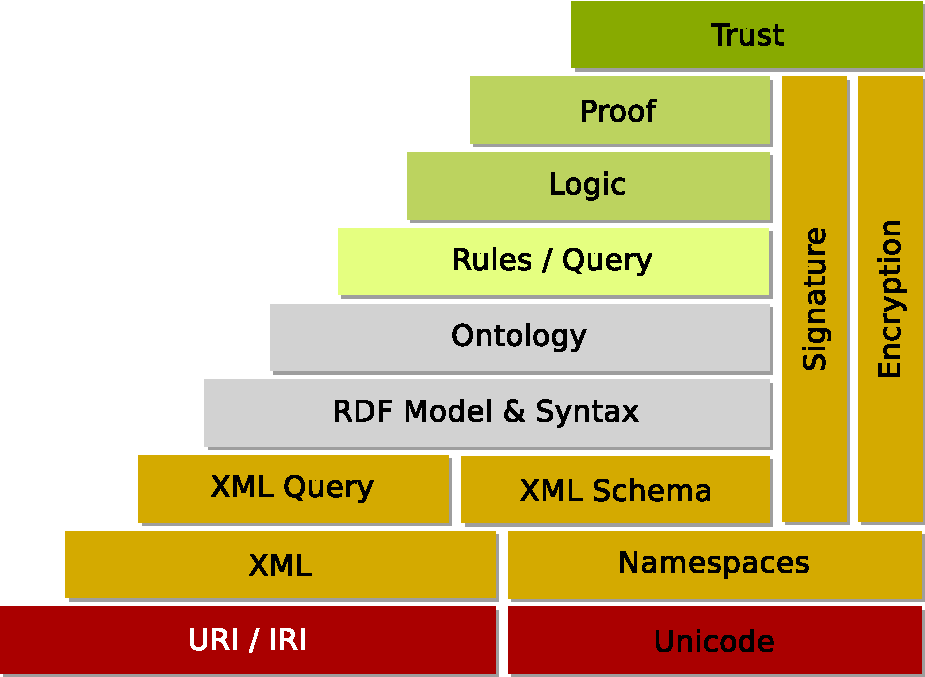
\includegraphics[width=0.6\textwidth]{img/pdf/w3c-semantic-web-layers.pdf}
      \begin{tablenotes}\footnotesize
      \item [~] Quelle: \url{en-wiki:File:W3c-semantic-web-layers.svg}
      \end{tablenotes}   
    \end{threeparttable}
    \caption[]{Die Komponenten des \emph{Semantic Web Stack}}
  \end{figure} 


\paragraph{}
Aus Platzgründen werden URIs oft mit Namensraum-Präfixen abgekürzt.
In dieser Arbeit ist beispielsweise \prefix{dbpedia} als Abkürzung für \url{http://dbpedia.org/resource/} definiert.
Dadurch können wir anstelle von \url{http://dbpedia.org/resource/London} nur \url{dbpedia:London} schreiben.
Die in dieser Arbeit verwendeten Namensraum-Präfixe befinden sich in Tabelle \ref{tab:namespace-prefixes}.
\paragraph{}
Es existieren folgende Unterarten von URIs:
\begin{itemize}
 \item \emph{Uniform Resource Locators (URLs)} identifizieren eine Ressource über ihren Zugriffsmechanismus. Sie sind also für eine Maschine erreichbare Ressourcen, wie zum Beispiel Webseiten.
Dies hat den Vorteil, dass zusätzliche Informationen über eine Ressource erhalten werden können, indem die URL dereferenziert wird.
\url{http://dbpedia.org/resource/London} dient also sowohl als eindeutige Identifikation als auch als Angabe, 
wie eine Maschine herausfinden kann, wie viele Einwohner London hat oder welche Flughäfen sich in der Stadt befinden.
 \item \emph{Uniform Resource Names (URNs)} sind dagegen dauerhafte, ortsunabhängige Ressourcenbezeichner mit dem Schema \emph{urn}. So identifiziert beispielsweise \url{URN:ISBN:0-671-43241-9} das Buch
\emph{The Hitchhiker's Guide to the Galaxy}, ohne jedoch anzugeben, wo man dieses Buch finden kann.
\end{itemize}
Ein Konzept kann sowohl durch eine oder mehrere URLs als auch durch eine oder mehrere URNs identifiziert werden.
Weiterhin gibt es URIs, die weder URLs noch URNs sind, zum Beispiel \url{mailto:max_mustermann@yahoo.com}.

\subsection{Das Resource Description Framework}
Das \emph{Resource Description Framework} (RDF, engl. (sinngemäß) „System zur Beschreibung von Ressourcen“) wird dazu genutzt, Informationen im Semantischen Web zu repräsentieren \citep{www-rdf}.
Es besteht aus einem \emph{semantischen Datenmodell}, um beliebige wahre Aussagen über Ressourcen zu treffen, und einem
grundlegendem \emph{Vokabular}, mit dem den Aussagen eine Bedeutung zugeordnet werden kann.
Da RDF für das Web gedacht ist, werden Konzepte mit URIs identifiziert.
Weiterhin unterstützt RDF anonyme Ressourcen und Literale wie Zeichenketten und Zahlen.
Eine Aussage in RDF ist ein Tripel aus \emph{Subjekt}, \emph{Prädikat} und \emph{Objekt}, die folgende Werte annehmen können:
\begin{center}
\begin{tabular}{lccc}
\toprule
		&URI		&Anonym			&Literal\\
\midrule
Subjekt		&\checkmark	&\checkmark\\
Prädikat	&\checkmark\\
Objekt    	&\checkmark	&\checkmark      	& \checkmark\\
\bottomrule
\end{tabular} 
\end{center}
Damit ähnelt eine RDF-Aussage einem stark vereinfachten deutschen Satz, zum Beispiel aus einer Leselernfibel.
Eine natürliche Sprache ist zwar ausdrucksstärker aber dafür nicht geeignet, denn sie ist inhärent mehrdeutig.\footnote{Beispiel: "`Ich habe nicht gesagt, sie hat das Geld gestohlen."'}
RDF nimmt also eine beschränkte Aussagekraft in Kauf, um eine möglichst einfache Verarbeitung zu ermöglichen.
Da ein Objekt eines Tripels das Subjekt eines anderen Tripels sein kann, lässt sich ein Tripel als Kante
in einem gerichteten, beschrifteten Graph auffassen.
Daher nennt man eine Menge von Tripeln auch einen \emph{Graphen}. 
Anonyme Ressourcen werden oft als \emph{blank nodes} bezeichnet.
\paragraph{Syntaxen}
Das RDF-Datenmodell ist eine abstrakte Syntax und damit unabhängig von einer bestimmten Darstellung.
Es gibt jedoch mehrere konkrete Syntaxen, wie zum Beispiel Turtle, RDF/XML und N3,  die in Ausdrucksstärke, menschlicher Lesbarkeit und Softwareunterstützung variieren.
Auch zum Speichern und Verwalten von RDF-Daten gibt es mehrere Möglichkeiten, \zb als Textdatei, auf einer Webseite oder in einem \emph{Triple Store}, dem RDF-Äquivalent einer Datenbank.

\begin{bsp}
Im vorigen Abschnitt wurden RDF-Statements mit den einfachen Sätzen in einer Leselernfibel verglichen.
Die folgenden drei Sätze lassen sich als Graph ausdrücken, indem für die Substantive und Verben URIs eingeführt werden:
\begin{itemize}
\item{"`Lilo mag Moni"'}
\item{"`Max sagt Ball"'}
\item{"`Susi sieht Sonne"'}
\end{itemize}
Als RDF-Graph:\\
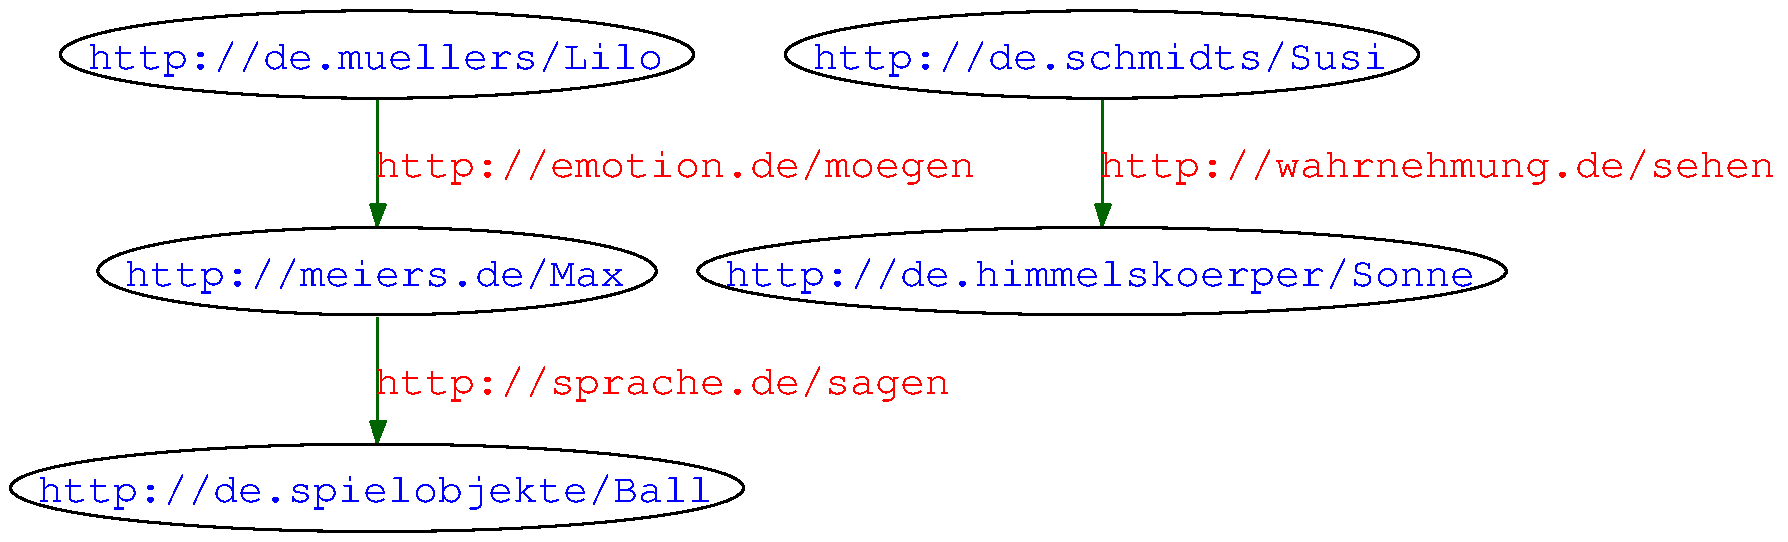
\includegraphics[width=\textwidth]{img/pdf/fibel_fontsize_20.pdf}\\
In N3:
\begin{itemize}
\item{\url{muellers:Lilo} \url{emotion:moegen} \url{meiers:Max}.}
\item{\url{muellers:Max} \url{sprache:sagen} \url{spielobjekte:Ball}.}
\item{\url{schmidts:Susi} \url{wahrnehmung:sehen} \url{himmelskoerper:Sonne}.}
\end{itemize}
 
\end{bsp}
% Um Information in einer für Maschinen verarbeitbaren Form darzustellen, benötigt man eine formale Sprache.
% 
% Weiterhin ist ihre Aussagekraft einfach zu groß.
% Es mag zwar paradox anmuten, dass eine große Ausdrucksfähigkeit einer Sprache zum Nachteil gereichen kann, doch erschwert sie die Validierung einer Aussage,
%  ja sie kann sie sogar unmöglich machen\footnote{Beispiel: "`Ich lüge jetzt."'}.
% Es muss also ein Kompromiß gefunden werden zwischen möglichst großer Ausdruckskraft auf der Einen und möglichst einfacher Verarbeitung der damit bildbaren Aussagen auf der anderen Seite.
% RDF nimmt dabei eine sehr beschränkte Aussagekraft in Kauf, um eine möglichst einfache Verarbeitung zu ermöglichen.
% Wenn wir eine möglichst einfache Untermenge unserer Sprache suchen, so erinnern wir uns sicher noch an unsere Grundschulzeit zurück und an das Lesenlernen mit einer Fibel.
% Die dort enthaltenen Sätze haben meist ein ganz einfaches Format:
% \begin{itemize}
% \item{"`Lilo mag Moni"'}
% \item{"`Max sagt Ball"'}
% \item{"`Susi sieht Sonne"'}
% \end{itemize}
% Sie besitzen ein Subjekt, ein Prädikat (Verb) und ein Objekt.
% Genau das ist RDF; da so eine Aussage aus genau drei Teilen besteht, spricht man auch von RDF-Tripeln.
% Allerdings sind die Bestandteile eines Tripels natürlich keine Wörter sondern URLs.
% Die drei Sätze würden also in RDF eher so aussehen:
% \includegraphics[width=\textwidth]{doc/latex/img/fibel_fontsize_20.ps}
% Ausgeschrieben:
% \begin{itemize}
% \item{\url{http://de.muellers/Lilo} \url{http://emotion.de/moegen} \url{http://de.meiers/Max}.}
% \item{\url{http://de.muellers/Max} \url{http://sprache/sagen} \url{http://de.spielobjekte/Ball}.}
% \item{\url{http://de.schmidts/Susi} \url{http://wahrnehmung/sehen} \url{http://de.himmelskoerper/Sonne}.}
% \end{itemize}
% Diese Notation nennt sich N3.


\iffalse
<?xml version="1.0"?>
<rdf:RDF  
xmlns:rdf="http://www.w3.org/1999/02/22-rdf-syntax-ns#"
xmlns:wahrnehmung="http://wahrnehmung.de/"
xmlns:emotion="http://emotion.de/"
xmlns:sprache="http://sprache.de/"
>
  <rdf:Description rdf:about="http://de.muellers/Lilo">
    <emotion:moegen rdf:resource="http://meiers.de/Max"/>
  </rdf:Description>
  <rdf:Description rdf:about="http://meiers.de/Max">
    <sprache:sagen rdf:resource="http://de.spielobjekte/Ball"/>
  </rdf:Description>
  <rdf:Description rdf:about="http://de.schmidts/Susi">
    <wahrnehmung:sehen rdf:resource="http://de.himmelskoerper/Sonne"/>
  </rdf:Description>
</rdf:RDF>
\fi
%Es gibt jedoch noch weitere Dateiformate, so kann man RDF genauso in einer Datenbank (Tripelstore) oder als XML (RDF/XML) abspeichern.

\subsection{SPARQL}
\emph{SPARQL} ist eine Abfragesprache für das Semantische Web \citep[siehe][]{www-sparql}.
Der Name ist ein rekursives Akronym für \emph{SPARQL Protocol and RDF Query Language}.
Der zentrale Part einer SPARQL-Anfrage besteht aus Tripelmustern, die mittels Konjunktionen und Disjunktionen miteinander verknüpft sind.
Diese Tripelmuster bestehen aus URLs und Variablen, die für das Subjekt, Prädikat und Objekt eines Tripels stehen.
Weiterhin muss die Abfrageart angegeben sein, welche die Werte \emph{SELECT}, \emph{CONSTRUCT}, \emph{ASK}, und
\emph{DESCRIBE} annehmen kann.
Einige SPARQL-Implementierungen definieren Erweiterungen für die SPARQL-Abfragesprache.
So bietet beispielsweise \emph{Virtuoso SPARQL} den Abfragemodus \emph{SELECT COUNT}, der nicht die zutreffenden Ergebnisse an sich, sondern nur deren Anzahl zurückgibt, was bei Anfragen dieses Typs 
einen deutlichen Geschwindigkeitsvorteil ermöglicht.
\begin{bsp}
\paragraph[]{Anfrage\footnote{\property{a} ist eine Abkürzung für \property{rdf:type}}}
\begin{verbatim*}
SELECT ?o WHERE
{
<http://dbpedia.org/resource/Ant> a ?o.
} 
\end{verbatim*}
\paragraph{Ergebnis}
\begin{verbatim*}
owl:Thing
<http://sw.opencyc.org/2008/06/10/concept/Mx4rvVjf5JwpEbGdrcN5Y29ycA>
dbpedia:ontology/Species
dbpedia:ontology/Animal
dbpedia:ontology/Insect
dbpedia:ontology/Eukaryote
\end{verbatim*}

\end{bsp}

\subsection{Linked Data}
Eine Webseite, die keine Links enthält und auf die nicht verlinkt wird, ist nutzlos.
Sie wird von einer Suchmaschine nicht gefunden und auch wenn man einen Artikel über ein ähnliches Thema liest, erfährt man nicht von der Existenz dieser Seite.
Das zentrale Element des WWW ist also die Verknüpfung durch Links. Diese sind jedoch nicht \textit{typisiert}, das heißt ein Link gibt nur an, dass irgendeine Art Beziehung existiert, aber nicht, welche das genau ist.
Ein menschlicher Benutzer kann anhand der Beschreibung im Text entscheiden, welchen Links er folgt und welchen nicht. 
Dies stellt jedoch ein enormes Problem für einen Agenten dar, der eine bestimmte Information sucht und herausfinden muss, welche der Links für ihn relevant sind.
\emph{Linked Data} löst dieses Problem, indem jeder Link zwischen zwei Entitäten einen bestimmten Typ hat.
%Analog dazu wird das enorme Potential des Semantischen Webs erst dann ausgereizt, wenn die darin enthaltene Information sinnvoll miteinander verknüpft wird.
Das Konzept geht auf einen Vorschlag von \citet{www-linked-data-proposal} zurück und legt auch die zu benutzenden Technologien fest.
Grundprinzipien sind:\footnote{Aus dem Englischen übersetzt aus \cite{www-linked-data-proposal}.}
\begin{enumerate}
\item{Benutze URIs als Namen für Dinge}
\item{Benutze HTTP URIs, damit menschliche Benutzer den Namen nachschlagen können}
\item{Stelle nützliche Information über eine URL in Form der Standards RDF und SPARQL zur Verfügung}
\item{Verlinke auf andere URIs, sodass der Benutzer andere Dinge entdecken kann}
\end{enumerate}
Während im WWW die Links, die von einem Dokument auf ein Anderes verweisen, in Ersterem enthalten sein müssen, kann Jedermann Linked Data über Dinge seiner Wahl bereitstellen,
und damit Verknüpfungen zwischen bereits existierenden Ressourcen erschaffen.
\iffalse
Je größer das Netzwerk und der Vernetzung dazwischen, desto wertvoller ist jede einzelne Ressource. Dies führt zu einem superlinearen Wachstum 
So wie ein Student, der sich stur Fakten um Fakten einverleibt, keinen Erfolg haben wird\footnote{Im Fachbereich Informatik jedenfalls\ldots},

Das Semantische Web besitzt ein beeindruckendes Potential.
Die Zahl der möglichen Anwendungen, die Auswirkungen auf die Informationstechnik und die vorstellbaren Veränderungen im Alltag jedes Einzelnen sind zwar gewaltig (im Guten wie auch im Bösen), 
doch leidet das Semantische Web an einem prinzipiellen Problem von Netzwerken:
Der Nutzen eines Netzwerkes für jeden Teilnehmer wächst mit der Größe des Netzwerkes. Zu Beginn ist der Anreiz, 
-> Metcalfesches Gesetz
Schier überwältigend ist die Zahl der möglichen Anwendungen des Semantischen Webs, des mögli
\fi

\subsection{Ontologie}
Eine \textit{Ontologie} ist eine formale Beschreibung einer Menge von Konzepten und der Beziehungen dieser Konzepte untereinander.
Eine Ontologie stellt ein gemeinsames Vokabular für ein bestimmtes Fachgebiet zur Verfügung und erlaubt es, Aussagen über die Merkmale dieses Fachgebietes zu treffen oder es zu definieren. 
%Sie beschreibt, welche Arten von Objekten und Konzepten existieren und wie diese zusammenhängen.
Eine Ontologie hat folgende Bestandteile:
\begin{itemize}
\item \emph{Instanzen} oder \emph{Individuen} sind die grundlegenden Objekte in der Ontologie, \zb{} \emph{London}.
\item \emph{Klassen} oder \emph{Typen} sind Mengen von Instanzen. \emph{London} ist ein Element der Klasse \emph{Stadt},
im Folgenden auch "`\emph{London} ist eine Instanz der Klasse \emph{Stadt}"' oder "`\emph{London} ist vom Typ \emph{Stadt}"'.
\item \emph{Literale} sind Werte wie Zahlen oder Zeichenketten.
\item \emph{Relationen} oder \emph{Properties} beschreiben die Beziehungen zwischen Klassen, Instanzen und Literalen.
\item \emph{Axiome} sind wahre Aussagen innerhalb der Ontologie die Wissen repräsentieren, \zb{} "`Zwischen London und Leipzig existiert eine Zugverbindung"'.
\end{itemize}

%Eine Ontologie über die grammatikalische Struktur von Sätzen könnte unter anderem definieren, dass ein \emph{Satz} aus \emph{Hauptsätzen} und \emph{Nebensätzen} \emph{besteht}, ein \emph{Hauptsatz} ein \emph{Subjekt} und ein \emph{Prädikat} \emph{enthält} und dass ein \emph{Personalpronomen} ein \emph{Pronomen} \emph{ist}.
Ontologien werden durch spezielle Beschreibungssprachen repräsentiert. 
Dabei existieren einige solcher Sprachen, wie \textit{RDFS}, \emph{OWL Lite}, \emph{OWL DL}, \emph{OWL Full} und \textit{OWL 2}, die sich in Ausdrucksstärke, Komplexität und Entscheidbarkeit unterscheiden.
Während es in RDFS beispielsweise erlaubt ist, das Klassen Instanzen von anderen Klassen sind, ist dies in OWL DL nicht möglich.
\iffalse
\paragraph{OWL}
OWL (Web Ontology Language) ist eine Beschreibungssprache für Ontologien. Sie verwendet die Syntax von RDF und lässt sich in drei verschiedenen Versionen benutzen.
\begin{itemize}
\item{OWL Lite}
\item{OWL DL}
\item{OWL Full}
\end{itemize}
Die hier verwendete Version ist OWL \todo{[insert here]}.
blabla
\fi

\subsection{Open World Assumption}
Liegt einem Auskunftssystem alle vorhandene Information über ein bestimmtes Thema vor, dann kann dies alle Anfragen, ob eine bestimmte, in diesem System formulierbare, Aussage gültig ist oder nicht, mit entweder ja oder nein beantworten.
Wenn ein Kinobesucher wissen möchte, ob er sich Freitag Abend \emph{Twilight -- New Moon} ansehen kann und im Spielplan zu dieser Zeit kein Eintrag existiert, dann kann ihm der Mitarbeiter mit Sicherheit sagen,
dass sich der Kunde diesen Film zu dieser Zeit leider nicht ansehen kann.
Dem Kinospielplan liegt also eine \emph{Closed World Assumption} (Geschlossene-Welt-Annahme) zugrunde.
Im Semantischen Web wird jedoch Weltwissen repräsentiert, welches an vielen verschiedenen Orten gespeichert und niemals vollständig ist.
Aussagen die nicht explizit vorliegen können also nicht bestätigt, jedoch auch nicht verneint werden.
Es gilt also die \emph{Open World Assumption} (Offene-Welt-Annahme).

%\subsection{Der DL-Learner}
%Der DL Learner\footnote{Projektseite \url{http://dl-learner.org/Projects/DLLearner}} ist ein Programm, welches Konzepte in Beschreibungslogiken, wie OWL, anhand von Beispielen lernt. Bei Eingabe von positiven und negativen Beispielen erzeugt er ein passendes OWL-Konzept, es sind jedoch auch andere Betriebsmodi möglich.
%Er ist in Java implementiert und steht unter einer Open Source Lizenz und ist damit sehr gut in andere Javaprogramme integrierbar.

\section{Grundbegriffe der Linguistischen Informatik}

Ein \definition{Parser} für natürliche Sprache ist ein Programm, dass die grammatikalische Struktur von Sätzen (die \emph{Morphologie}) bestimmt.
Ein Satz könnte beispielsweise in einen Hauptsatz und einen Nebensatz unterteilt werden, ein Wort als Subjekt gekennzeichnet werden, ein anderes als Objekt und ein weiteres als Verb.
Da die Grammatik einer natürlichen Sprache kompliziert und im allgemeinen NP-vollständig ist, sind die meisten Parser statistisch.
Statistische Parser benutzen als Trainingsmenge Texte einer bestimmten Sprache -- ein \definition{Korpus} -- die mit einer Menge von Tags -- einem \definition{Tagset} -- annotiert wurden.
Ein solches annotiertes Korpus nennt man auch \definition{Treebank}.

Ein Programm, das Sätze in seine Einzelteile (Tokens), dies sind Wörter und Satzzeichen, zerlegt, heißt \definition{Chunker}. %\footnote{Im Allgemeinen wird darunter auch die Identifizierung von Satzbestandteilen verstanden.}.
Ein \definition{Feature} bezeichnet eine beliebige Eigenschaft eines Satzes, zum Beispiel ob er ein ein Aktiv- oder ein Passivsatz ist oder ein Reflexivpronomen enthält.
Die \definition{Grundform} oder das \definition{Lemma} eines Wortes ist die Form, unter der man es in einem Nachschlagewerk findet
(ein Beispiel: \emph{getrunken} $\rightarrow$ \emph{trinken}).
Die \emph{Stammform} (englisch \emph{stem}) hingegen ist der Kern eines Wortes, der als Basis zur Bildung der gebeugten Wortform dient.
Der Stamm von \emph{trinken} wäre also \emph{trink}, aus dem sich dann die Formen \emph{trinke}, \emph{trinkst}, \emph{trinken}, \emph{trinkt} bilden lassen.

\iffalse
\paragraph{Textklassifikation}
Das Problem der Textklassifikation besteht darin, einen Satz oder ein elektronisches Dokument automatisch in eine oder mehrere Kategorien einzuteilen.
Man unterscheidet dabei zwischen überwachter, halbüberwachter und unüberwachter Klassifikation,
 je nachdem ob und in welchem Maß eine externe Quelle (\zb{} ein Mensch) Informationen über die korrekte Klassifikation beisteuert.
In dieser Arbeit sind diese Kategorien nur "`weist Merkmal x auf"' und "`weist Merkmal x \emph{nicht} auf"'.
\fi
\section{Wikipedia}
Wikipedia ist eine freie, Wiki-basierte Online-Universalenzyklopädie, die von DBpedia als primäre Datenquelle benutzt wird.
Durch die \emph{Creative-Commons-Lizenz} ist sie nicht nur kostenlos verfügbar sondern darf auch frei kopiert und verwendet werden.

\paragraph{Wiki}
ist das hawaiische Wort für schnell und bezeichnet eine Technik, die es einer großen Menge von Benutzern ermöglicht, gemeinsam Internetseiten zu erstellen.
Dabei gibt es sowohl firmeninterne, als auch frei zugängliche Wikis.
Der Durchbruch der Konzepts kam mit Wikipedia, mittlerweile gibt es jedoch viele weitere wiki-basierte Projekte, zum Beispiel Wikibooks und Wiktionary.
Das grundlegende Konzept ist, dass Benutzer Seiten ansehen und editieren können.
Trotz anfänglicher Befürchtungen hat sich dieser Ansatz aufgrund der aktiven Gemeinschaft als erstaunlich robust herausgestellt.
So wird beispielsweise die Hälfte aller Massenlöschungen in weniger als drei Minuten wieder rückgängig gemacht \citep[Seite 579]{wikipedia-vandalism}.
Sämtliche Versionen sind in einer Chronik gespeichert und können jederzeit wiederhergestellt werden.
Die Versionierung hat jedoch noch einen weiteren Vorteil:
So dienen ältere Versionen als dauerhafte Abbilder eines Artikels zu einem bestimmten Zeitpunkt.
In dieser Arbeit sind Verweise auf Seiten der Wikipedia deshalb mit ihrer Versionsnummer versehen.
Auch die Qualität des gemeinschaftlichen Ansatzes hat sich als hoch genug erwiesen, dass bereits gerichtliche Entscheidungen auf Basis von in Wikipediaartikeln enthaltenen Informationen gefällt wurden \citep*{wikipedia-formula-one}.

\paragraph{Artikel}
Der elementare Baustein von Wikipedia ist der Artikel.
Jeder dieser Artikel beschreibt ein bestimmtes Konzept, welches sowohl eine Klasse (\article{en-wiki:Human}) als auch eine Instanz (\article{en-wiki:Al_Pacino}) sein kann.
%Welche Arten von Konzepten jedoch genau durch Artikel beschrieben werden ist jedoch schwer zu definieren.
%Die Seite \article{en-wiki:Wikipedia:What is an article}\footnote{\url{http://en.wikipedia.org/w/index.php?title=Wikipedia:What_is_an_article?&oldid=347855498}} 
%nur "`A Wikipedia article is a page that has encyclopedic information on it"'.
In Abgrenzung von einem Wörterbuch ist ein enzyklopädischer Artikel in Wikipedia folgendermaßen beschrieben:\footnote{\url{http://en.wikipedia.org/w/index.php?title=Wikipedia:Wikipedia_is_not_a_dictionary&oldid=353213935}}
\begin{quote}
Each article in an encyclopedia is about a person, or a people, a concept, a place, an event, a thing etc.; whereas a dictionary article is primarily about a word, an idiom or a term and its meanings, usage and history.
\end{quote}

Als Abgrenzung eines Artikels zu einer anderen Seite der Wikipedia existiert die Definition:
"`Ein Artikel ist eine Seite, die im Artikelnamensraum liegt (kein Präfix), keine Weiterleitung ist und mindestens einen Wikilink enthält."'\footnotemark{}
\footnotetext{Übersetzt aus {\url{http://en.wikipedia.org/w/index.php?title=Wikipedia:What_is_an_article?&oldid=347855498}}}
Dies schließt auch Disambiguierungsseiten ein, die meist nur aus Wikilinks und deren Kurzbeschreibungen bestehen.
\paragraph{} 
Der Name eines Artikels auf ist gleich seinem Titel, wobei jedoch Leerzeichen durch Unterstriche ersetzt werden.
Ist der Artikel eine Disambiguierungsseite, dann wird der Name meist um ein "`\_(Disambiguation)"' (bzw. das Äquivalent in anderen Sprachversionen) erweitert.
Gibt es mehrere gleichnamige Artikel, dann wird sowohl an den Titel als auch an den Artikelnamen in Klammern der Kontext angehängt; wird eine Bedeutung im Sprachgebrauch jedoch häufiger benutzt,
kann dieser auch keine Klammern enthalten.
Ein Beispiel hierfür sind die Artikel \emph{Bank\_(Begriffsklärung)}, \emph{Bank} (dieser Artikel beschreibt das Kreditinstitut) und \emph{Bank\_(Möbel)}.
% "`A good encyclopedia article can and should begin with a relatively short but discrete explanation of what the subject of the article — the person, place, concept, event, or thing that its title denotes — is."'
% "`Wikipedia articles should begin with a good definition and description of one topic, however, they should provide other types of information about that topic as well."'
% http://en.wikipedia.org/w/index.php?title=Wikipedia:Wikipedia_is_not_a_dictionary&oldid=353213935
%\paragraph{Qualität}
%Während dies bei einem normalen Artikel noch nicht dem Anspruch einer zitierfähigen Quelle gerecht wird, kann bei Seiten des 
%In Wikipedia gibt es zu jedem Artikel eine Diskussionsseite, in der über geplante Änderungen diskutiert wird.
%Entscheidungen werden in einem gemeinsamen Prozess gefällt.

\section{DBpedia}
Das \textit{DBpedia}-Projekt extrahiert strukturierte Informationen aus Wikipedia-Artikeln und 
stellt diese frei im Web zu Verfügung. 
DBpedia ist also der Semantic-Web-Gegenpart zu Wikipedia.
Die durch das Projekt generierten RDF-Daten repräsentieren eine Teilmenge der in den Wikipedia-Artikeln enthaltenen Informationen.
Die extrahierten Daten sind mit der zu diesem Zweck erstellten DBpedia-Ontologie klassifiziert. Durch das \emph{Linking Open Data}-Projekt wurde DBpedia jedoch auch mit den
Wissensquellen YAGO und Open-Cyc verlinkt, wodurch zusätzliche Klassifikationsschemata bereitstehen.
%Die Daten werden dann als Linked Data und über SPARQL-Interfaces veröffentlicht.
Die große Errungenschaft von DBpedia ist, dass sie einen Teil der unermesslichen Informationsfülle von Wikipedia
für das Semantische Web zur Verfügung stellt und damit den Nutzen vieler Anwendungen erhöht oder sie erst möglich macht.
Dies macht DBpedia zu einer der zentralen Verknüpfungsstellen der \emph{LOD-Cloud}, der Menge der vom \emph{Linking Open Data Project} \citep{lod} verlinkten Wissensquellen, und leistet damit einen entscheidenden Beitrag, um das Wachstum des Semantic Web in Gang zu bringen.
\begin{figure}[h]
\begin{center}
\begin{threeparttable}
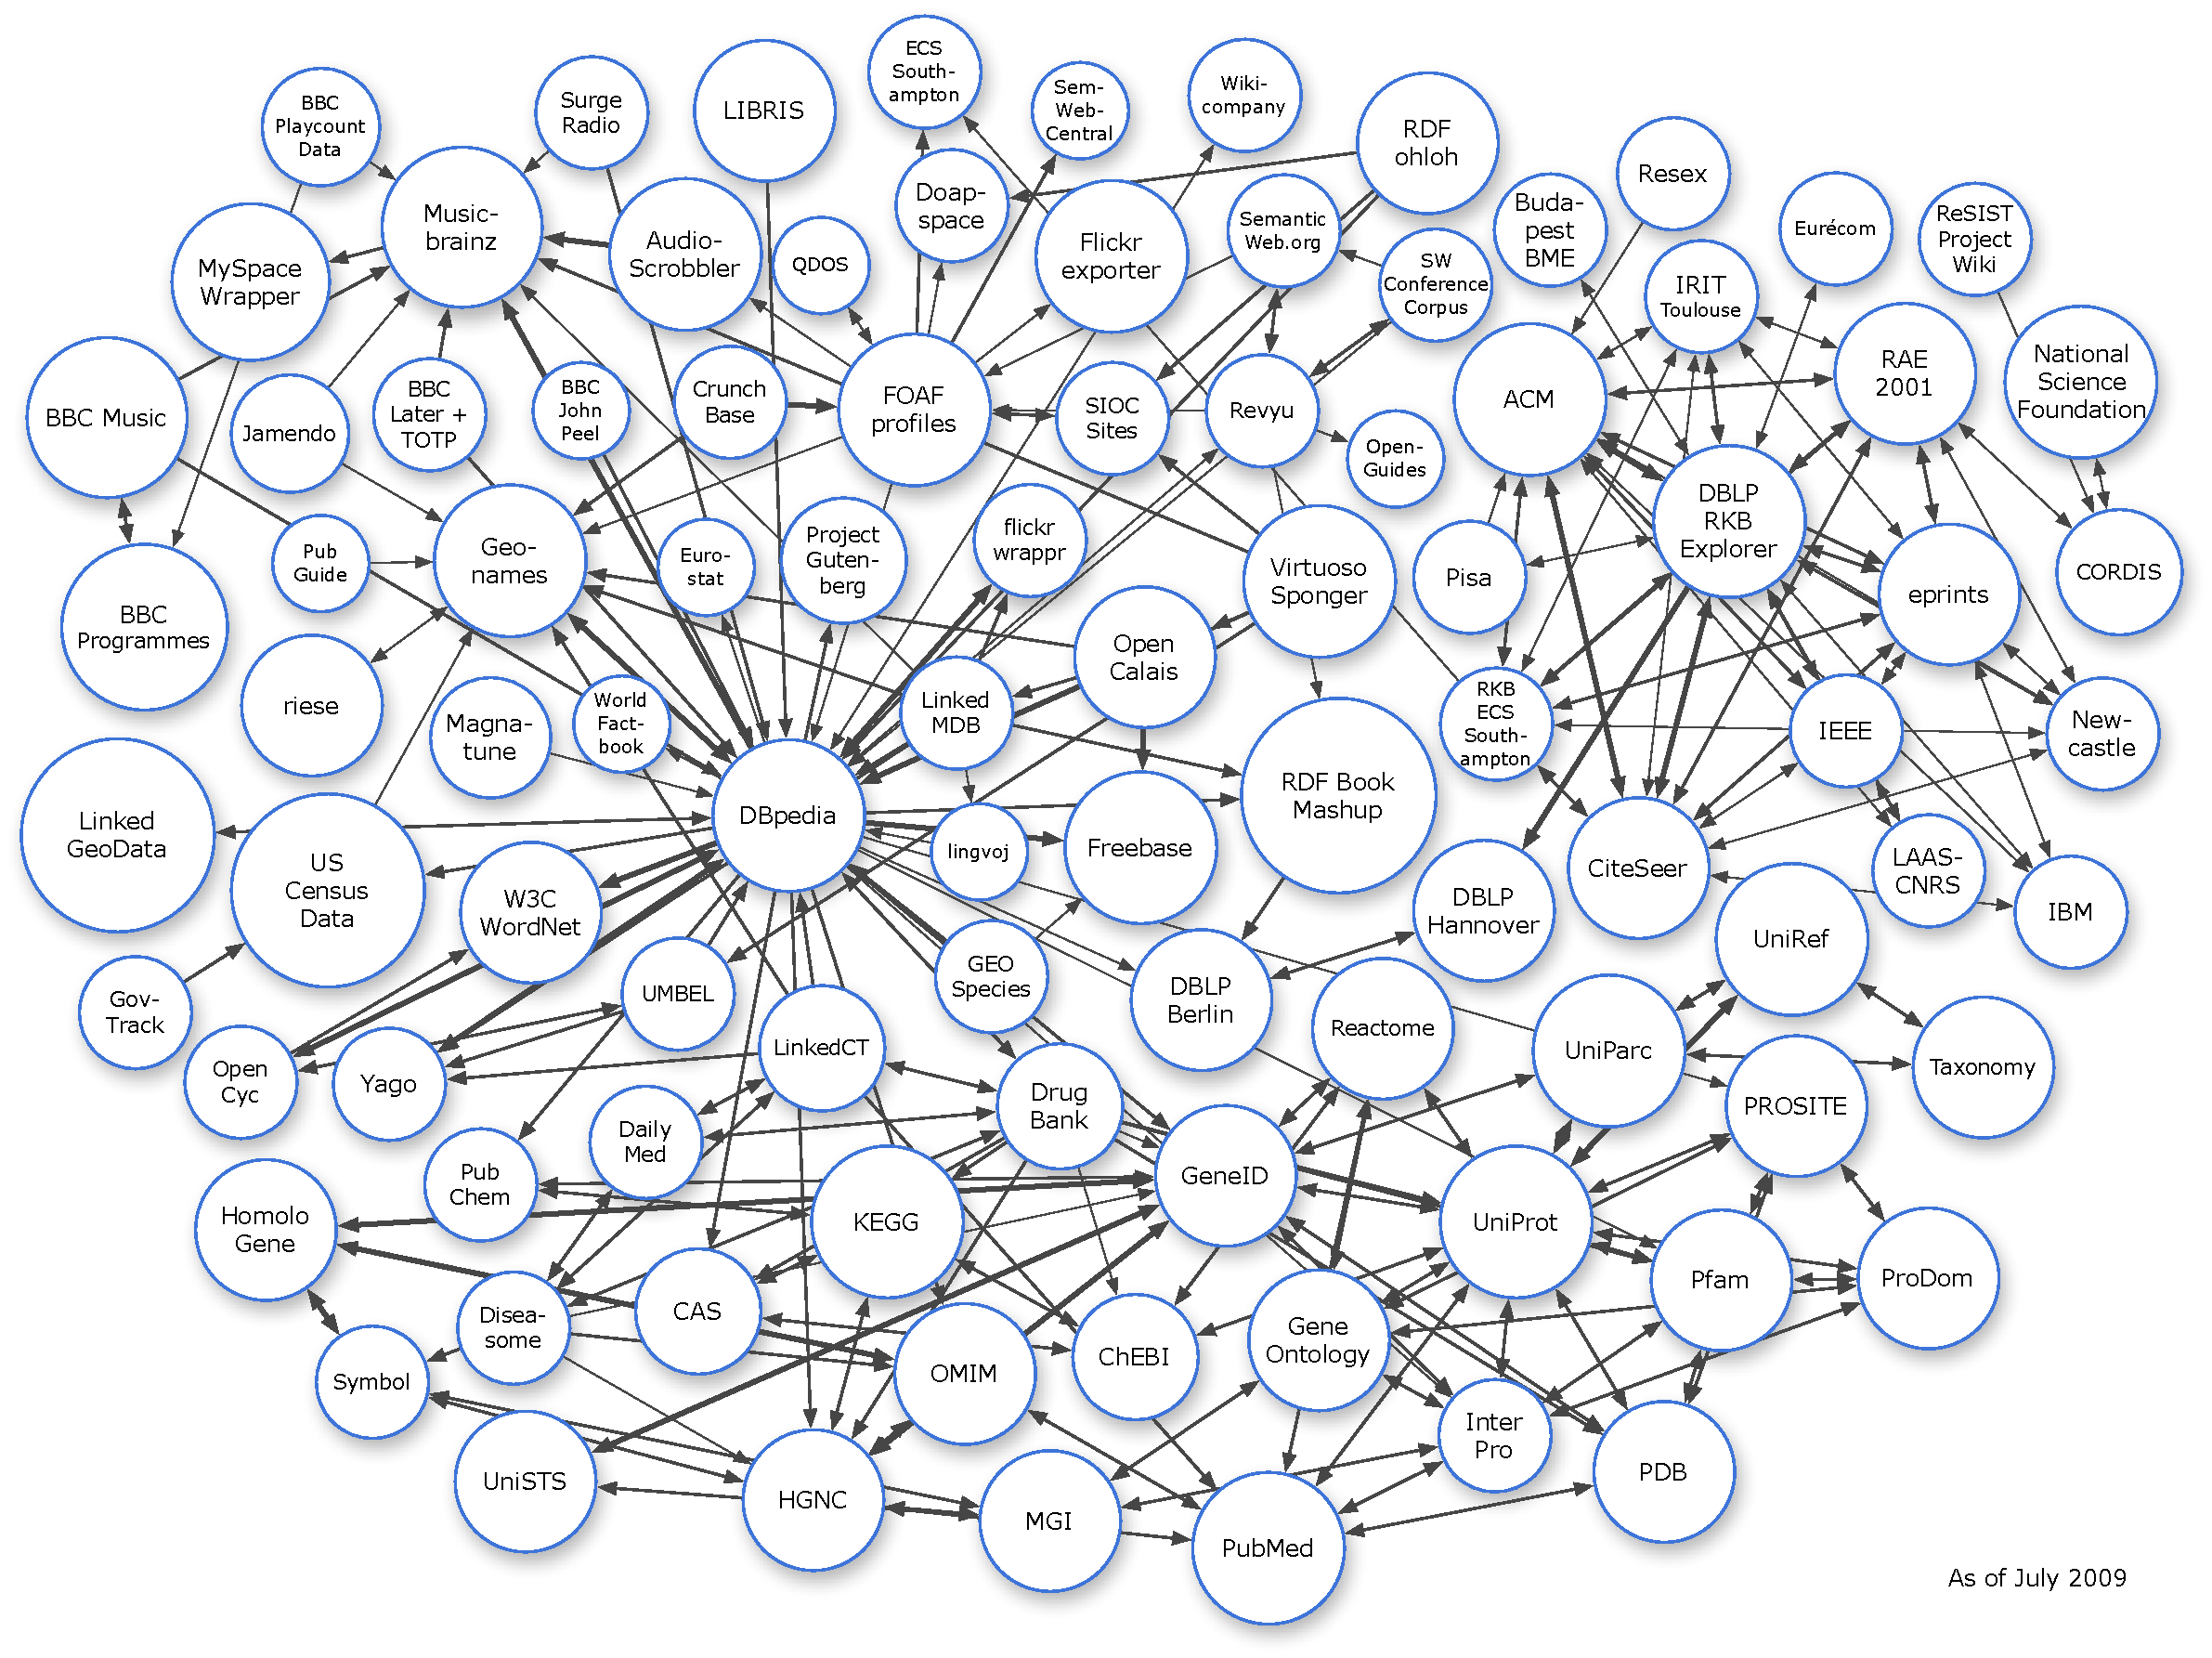
\includegraphics[width=\textwidth]{img/pdf/lod-cloud.pdf}
\begin{tablenotes}
\item [] \begin{footnotesize} Quelle: \url{http://richard.cyganiak.de/2007/10/lod/lod-datasets_2009-07-14.pdf}\end{footnotesize}
\end{tablenotes}
\end{threeparttable}
\end{center}
\caption{die LOD-Cloud}
\end{figure}
Die Daten von DBpedia sind via Download, \emph{Virtuoso SPARQL}- und Linked Data-Interface verfügbar.
Abbildung \ref{fig:dbpedia-pig} zeigt eine DBpedia-Entität als HTML-Sicht des Linked Data-Interfaces.
Die drei wesentlichen Bestandteile des DBpedia-Projektes sind die Webseite, die Datensets und das Extraktions-Framework.
Unter den Datensets ist jenes, das aus der englischen Wikipedia extrahiert wurde das Wichtigste.
Darin existiert zu jedem Wikipedia-Artikel \article{en-wiki:Articlename} eine RDF-Entität \article{dbpedia:Articlename}.
Informationen aus den entsprechenden Artikeln anderer Sprachversionen werden jedoch auch unter dem Namen des englischen Artikels von der DBpedia zur Verfügung gestellt.
\iffalse
The DBpedia ontology has been created for the purpose
of classifying this extracted data. In the course of the Linking Open Data project, DBpedia be-
came interlinked with other knowledge bases, namely YAGO, SKOS, UMBEL and Open-Cyc,
serving as additional classification schemata. This step cleared the path for DBpedia to become
one of the most important linking hubs within the LOD-cloud.
\fi
%Notably the latter two are powered by OpenLink’s Virtuoso Universal Server. -> eigentlich nicht interessant hier
%fig:dbpedia-pig

\iffalse
\section{LOD-Cloud}
\begin{quote}
Linked Data is about using the Web to connect related data that wasn't previously linked, or using the Web to lower the barriers to linking data currently linked using other methods.
More specifically, Wikipedia defines Linked Data as
"`a term used to describe a recommended best practice for exposing, sharing, and connecting pieces of data, information, and knowledge on the Semantic Web using URIs and RDF."'
\end{quote}

-> \todo{ein ordentliches eps finden}
\begin{center}
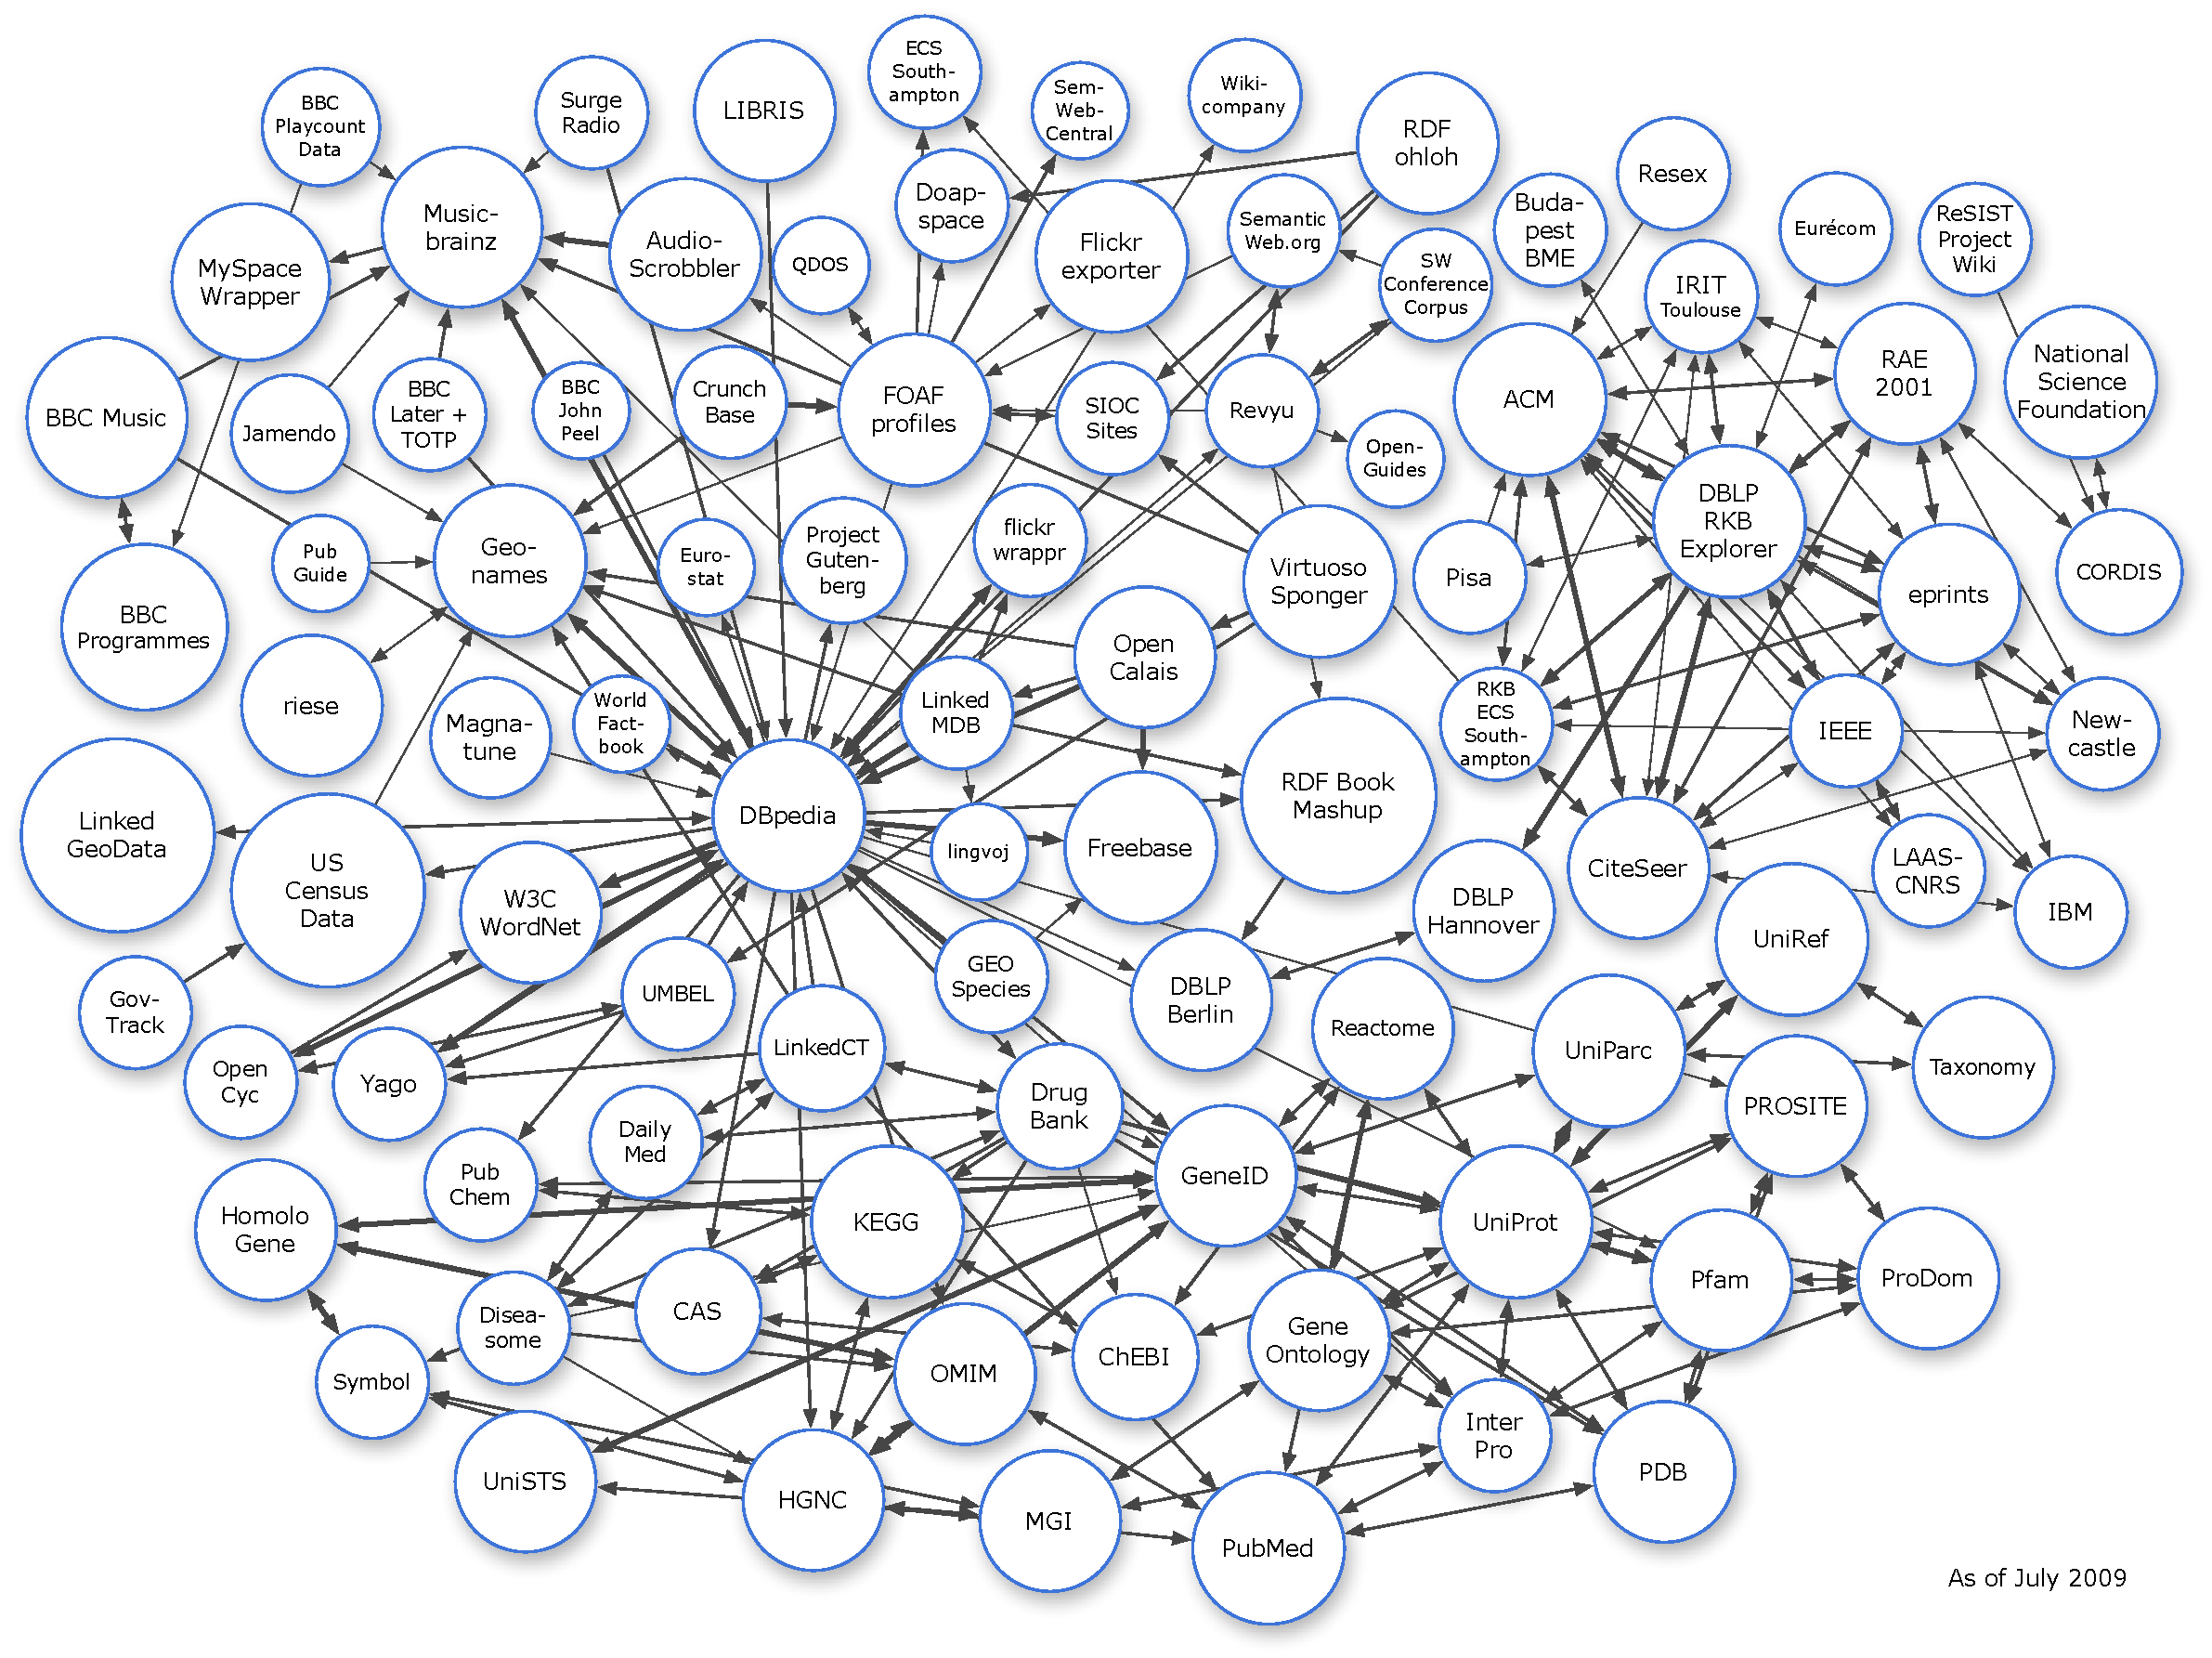
\includegraphics[width=\textwidth]{img/pdf/lod-cloud.pdf} 
\end{center}
\fi

\iffalse
\subsection{Mathe}
Zu (i) folgenden Lösungsansatz:
Seien $ w_1, w_2 \in W*, v \in V* $
$ f*(w_1 + w_2)(v) = (w_1 + w_2)(f)(v) = (w_1 \circ f)(v) + (w_2 \circ f)(v) = f*(w_1)(v) + f*(w_2)(v) $
$ \Rightarrow f*(w_1) + f(w_2) $

------------
Zu (ii)
Zz.: $ ker(f*) = im(f)^\perp $

$ ker(f*) \subseteq im(f)^\perp $
Sei $ l \in ker(f*) $ und $ v \in V $
$ \Rightarrow f*(l)(v)=0 \forall v \in V $
$ \Rightarrow (l \circ f)(v)=0 \forall v \in V $
$ \Rightarrow l(f(v))=0 \forall v \in V $
$ \Rightarrow l(w)=0 \forall f(v)=w \in W $
$ \Rightarrow l \in im(f)^\perp $

$ ker(f*) \supseteq im(f)^\perp $
$ \Rightarrow l(w)=0 \forall w \in W $
$ \Rightarrow l(f(v))=0 \forall v \in V $
$ \Rightarrow (l \circ f)(v)=0 \forall v \in V $
$ \Rightarrow f*(l)(v)=0 \forall v \in V $
$ \Rightarrow l \in ker(f*) $
\fi

\subsection{Grundbegriffe der Graphentheorie}
Mit $[A]^k$ bezeichnen wir die Menge aller k-elementigen Teilmengen von A.
Ein \emph{Graph} ist ein Paar $G = (V, E)$ disjunkter Mengen (von \emph{Ecken} und \emph{Kanten}) mit $E \subseteq [V]^2$; die Elemente von E sind also 2-elementige Teilmengen von V.
Ein Graph, der keinen Kreis enthält, ist ein \emph{Wald}.
Ein zusammenhängender Wald ist ein \emph{Baum}.
Einen \emph{Baum} mit fest gewählter Wurzel nennt man einen \emph{Wurzelbaum}.
Ein gerichteter Graph ist ein Paar $(V, E)$ disjunkter Mengen zusammen mit zwei Funktionen
init$: E \rightarrow V$ und 
ter$: E \rightarrow V$, die jeder Kante $e$ eine Anfangsecke init$(e)$ und eine Endecke ter(e) zuordnen;
die Kante $e$ heißt dann von init$(e)$ nach ter$(e)$ gerichtet.
Die obigen Definitionen stammen aus \citet{graphentheorie}.
Ein gerichteter Graph, der keinen Kreis enthält heißt auch \emph{DAG} (engl. \emph{directed acyclic graph}).
Ein \emph{gerichteter Wurzelbaum} ist ein zusammenhängender DAG mit einer fest gewählten Wurzel.
Es gibt zwei Arten von gerichteten Wurzelbäumen: bei \emph{Out-Trees} ist jeder Knoten über einen Pfad von der Wurzel aus erreichbar, bei \emph{In-Trees} ist die Wurzel über einen Pfad von jedem Knoten aus erreichbar.

\subsection{Grundbegriffe der Ordnungstheorie}
Eine Halbordnung ist eine zweistellige Relation "`$\leq$"' auf einer Menge M mit folgenden Eigenschaften:%$\leq\ \subseteq M \times M$
\begin{center}
\begin{tabular}{ll}
\toprule
Reflexivität	&$x \leq x, \forall x \in M$\\
Transitivität	&$(x \leq y \land y \leq z) \rightarrow (x \leq z), \forall x,y,z \in M$\\
Antisymmetrie	&$(x\leq y \land y\leq x) \rightarrow x=y, \forall x,y \in M$\\
\bottomrule
\end{tabular} 
\end{center}
$x < y$ ist eine Abkürzung für $x \leq y \land x \neq y$.
%Eine Relation $R$ ist \emph{reflexiv}, wenn gilt $x \leq x, \forall x \in M$, \emph{transitiv}, wenn gilt $(x \leq y \land y \leq z) \rightarrow (x \leq z), \forall x,y,z \in M$) und antisymmetrisch, wenn gilt $(x\leq y \land y\leq x) \rightarrow x=y, \forall x,y \in M$.
%Wichtige Eigenschaftsbegriffe für Relationen sind:
Zu einer beliebigen zweistelligen Relation $R \subseteq M \times M$ lässt sich die \emph{transitive Hülle} $R^+$ bestimmen, die die Relation $R$ um die Paare erweitert, die zur Einhaltung der Transitivität nötig sind.
Sie ist definiert als: $x \ R^{+} \ y : \Leftrightarrow \exists n \geq 0 \ \exists e_1,\dots ,e_n \in V: x \,R \,e_1 \,R \,e_2 \,R \dots \,R \,e_n \,R \,y$.


\subsection{Hierarchien in DBpedia}\label{sec:grundlagen-hierarchien}
Eine Hierarchie ist eine Anordnung von Klassen, welche einander über- oder untergeordnet sind.
Ist Klasse $A$ Klasse $B$ übergeordnet, dann heißt $A$ "`\emph{Superklasse} von $B$"' und $B$ "`\emph{Subklasse} von $A$"'.
Ist ein Individuum Instanz einer Klasse, dann ist es auch Instanz deren Superklassen.\footnote{Hierarchien, in denen Klassen welche selbst wieder Instanzen von Klassen sein können, werden in dieser Arbeit nicht betrachtet.}
Die Subklassenrelation entspricht also der Teilmengenrelation $\subseteq$ und ist damit eine Halbordnung.
%Die Superklassenrelation enhält dann das Paar $(A,B)$, die Subklassenrelation das Paar $(B,A)$.
In der Praxis wird nur die Relation der direkten Subklassen verwaltet, die Subklassenrelation ist dann die transitive Hülle der direkten Subklassenrelation.
Dieses Verfahren kann auch bei der Klassenzugehörigkeit eines Individuums angewandt werden, eine vollständige Angabe der Klassenzugehörigkeit heißt auch \emph{expandiert}.
%Aus Gründen der Speicherplatz-, Rechenzeit- und Darstellungsplatzersparnis werden im praktischen Einsatz nur die direkten Sub- oder Superklassen angegeben und verwaltet, die Super- und Subklassenrelationen sind dann die transitiven Hüllen super$^+$ und sub$^+$ der direkten Sub- und Superklassenrelationen super und sub.
%Da die Teilmengenrelation $\subseteq$ eine Halbordnung ist, ist der Graph der Sub- und Superklassenrelation 
%Der Graph der direkten Sub- und Superklassenrelation entspricht dann der \emph{Minimalrepräsentation}, also der \emph{transitiven Reduktion} dieses Graphen und ist damit auch ein DAG.
Besitzt die Hierarchie eine \emph{Wurzel}, dann gibt es eine allen Klassen gemeinsame Oberklasse.%, es gilt also super$^+(O,K)$ für alle Klassen $K$.
Ein Spezialfall der Hierarchie ist die \emph{Monohierarchie}, bei der die direkte Subklassenrelation einen In-Tree bildet,
eine \emph{Polyhierarchie} bezeichnet eine Hierarchie, bei der dies nicht der Fall sein muss.% Bei einer Polyhierarchie ist es also möglich, dass ein 

%Ein Spezialfall der Hierarchie ist die \emph{Monohierarchie}, bei der die direkte Sub- und Superklassenrelation einen gerichteten Wurzelbaum bildet.
%Bei der Angabe der Klassenzugehörigkeit einer Entität können enweder nur die unmittelbar zugeordneten oder sämtliche übergeordneten Klassen angegeben werden, der letztere Fall wird im Folgenden auch als \emph{expandierte Klassenzugehörigkeit} benannt.
%Eine Hierarchie, die keine Monohierarchie ist, heißt auch \emph{Polyhierarchie}.

%Besitzen manche Elemente mehrere direkte Superklassen, handelt es sich um eine \emph{Polyhierarchie}.
\iffalse
\begin{dfn}
Eine Hierarchie ist ein DAG $G = (V,\subseteq)$, wobei $V$ die Menge der \emph{Klassen} und $\subseteq$ die Superklassenrelation ist.
Es gilt also: $(e_1,e_2) \in E$ gdw. $e_1$ ist eine Superklasse von $e_2$.
%Dabei existiert genau eine Wurzel, das heißt eine Klasse, welche keine Superklasse besitzt.

Eine Monohierarchie ist sogar ein Baum.
\end{dfn}
\fi
\paragraph{Wikipediakategorien}%SKOS
In der Wikipedia kann jeder Artikel durch die Benutzer manuell einer oder mehreren Kategorien zugeordnet werden.
Diese Kategorien können nun selbst wieder Kategorien zugeordnet werden und bilden annähernd eine Polyhierarchie mit einer einzelnen Wurzel \url{Contents}.
%Das Kategoriensystem der Wikipedia ist also ein Thesaurus, das heißt eine Menge von Schlüsselwörtern, die mit Relationen (in diesem Fall \emph{ist Unterkategorie von } und \emph{ist Oberkategorie von}) verbunden sind.
Aufgrund der großen Menge an Kategoriendaten\footnotemark{} sind zu fast jedem Artikel semantische Daten verfügbar.
\footnotetext{Zum Zeitpunkt dieser Arbeit sind es 410618 Zuordnungen}
Da sich die Kategorien jedoch nicht nur auf die Artikelgegenstände, sondern auch auf die Artikel selbst beziehen können, sind nicht alle davon für einen
taxonomischen Vergleich der Artikelgegenstände nützlich, so \zb{} \emph{Wikipedia:Gesprochene\_Artikel} oder \emph{Wikipedia:Exzellent}.
Weiterhin sind die Daten teilweise unsauber, sodass Zyklen enthalten sind.

\paragraph{YAGO}
\citep[beschrieben in][]{yago} ist eine Polyhierarchie mit einer einzigen Wurzel namens \url{Entity} und verbindet die große Anzahl von Konzepten der Wikipedia mit der sorgfältig gepflegten Hierarchie von WordNet \citep{wordnet} um eine hochqualitative Hierarchie zu erzeugen.
Dabei enthält YAGO über \val{150000} Klassen.%Relationen, wobei sowohl Taxonomische ("`ist ein"') als auch nichttaxonomische Relationen enthalten sind.
%159375
\paragraph{DBpedia-Klassen}%owl-ontology
Eine weitere Hierarchie basiert auf der Extraktion von Klassen aus Wikipedia-Infoboxen.
So wird manuell einigen Infoboxtypen eine zugehörige Klasse zugeordnet.
Weist ein Artikel beispielsweise die Infobox "`Filmdaten"' auf, so wird dieser Artikel der Klasse \url{http://dbpedia.org/ontology/Film} zugewiesen.
Diese von Hand erstellte Hierarchie enthält nur 199 Klassen und bildet eine Monohierarchie mit der Wurzelkategorie \url{owl:Thing}. Die zugehörigen Daten sind sehr präzise, da Infoboxtypen sehr spezifisch sind.
 
\section{Projekt Deutscher Wortschatz}\label{sec:wortschatz}
Das \emph{Projekt Deutscher Wortschatz} der Universität Leipzig bietet statistische Informationen über Wörter aus einer Vielzahl von Sprachen
und wurde 1994 unter der Leitung von Uwe Quasthoff gestartet.
Mit je über 9 Millionen Sätzen ist das Wortschatzkorpus eines der größten Korpora in Deutsch, Englisch und Italienisch,
weiterhin existieren noch kleinere Korpora in anderen Sprachen.
Die gespeicherten Sätze stammen "`zum größten Teil aus Zeitungstexten, zu einem geringeren Teil auch aus
Fachtexten oder speziellen Wortlisten"' \cite[Seite 1]{wortschatz}.
Aus urheberrechtlichen Gründen werden die Texte jedoch satzweise und nicht als ganzer Artikel verwaltet.
Zu jeder Wortform ist eine Vielzahl an Informationen verfügbar, unter anderem die \emph{Frequenz}, \emph{Frequenzklasse}, \emph{Nachbarn}, \emph{Kookurrenzen} und \emph{Beispielsätze}.
In dieser Arbeit wird sowohl die Frequenz als auch die Frequenzklasse genutzt.
\paragraph{}
Die \textbf{Frequenz} bestimmt die Häufigkeit eines Wortes, sie ist definiert als die Anzahl der Sätze im Korpus, in denen die Wortform vorkommt.
\paragraph{}
Die \textbf{Frequenzklasse} bestimmt die Seltenheit eines Wortes und ist eine ganzzahlige Funktion der Frequenz; sie steigt wenn diese fällt.
Die häufigsten Wörter haben die Frequenzklasse 0, während die seltensten Wörter in der größten Frequenzklasse liegen.
Dabei macht man sich zunutze, dass in natürlichen Sprachen einige wenige Wörter sehr häufig, sehr viele Wörter jedoch sehr selten vorkommen.
Abbildung \ref{fig:zipf_wortschatz} zeigt, wie sich die Verteilungen der Frequenzen der Wörter von zwei Korpora des Wortschatzes verhalten.
Es kann nachgewiesen werden (hier exemplarisch an einem 1 Million Sätze großen englischen Normkorpus), dass sie dem \emph{Zipfschen Gesetz} \citep{zipf} entsprechen.
Es besagt: Ordnet man die Elemente absteigend nach ihrer Frequenz $f$, wobei der Rang $r$ die Position in der Reihenfolge angibt (das erste Element besitzt also den Rang 1), dann gilt:
\begin{equation*}
f \propto \frac{1}{r}
\end{equation*}
und damit:
\begin{equation}
f = f_{\max} \cdot \frac{1}{r}
\label{eqn:zipf}
\end{equation}
Eine solche Funktion ist jedoch sehr schwer zu erkennen, da der Wertebereich viele Größenordnungen umfasst und die Werte daher sehr nahe bei den Achsen liegen.
Aus diesem Grund sind die Abbildungen \ref{fig:zipf_wortschatz}, \ref{fig:zipf_wortschatz_with_expected_values} und \ref{fig:zipf_wortschatz_frequency} doppelt logarithmisch dargestellt.
Nun nutzt man aus, dass die Potenzfunktion $f_{\max} \cdot r^{-1}$ auf einer doppelt logarithmischen Darstellung als Gerade sichtbar ist\footnotemark{} und kann damit bestätigen,
dass die Frequenzverteilung der Wörter des englischen Korpus dem Zipfschen Gesetz annäherungsweise entspricht (siehe Abbildung \ref{fig:zipf_wortschatz_with_expected_values}).
\footnotetext{$\log_b(f_{\max} \cdot (b^r)^{-1}) = \log_b(f_{\max})+\log_b((b^r)^{-1}) = \log_b(f_{\max})-r$ für jede Basis $b$}

Dieses Zusammenhang wird nun genutzt, um die Grenzen der Frequenzklassen festzulegen. Dabei ist das Ziel, dass sich die Wörter eines Textes möglichst gleichmäßig auf die verschiedenen
Klassen verteilen, also gilt: $\displaystyle \sum_{w \in C_i} f(w) \approx \sum_{w \in C_j} f(w)$ (denn die Frequenz ist ja proportional zur Wahrscheinlichkeit, dass ein Wort in einem Text ein bestimmtes Wort ist).
Da eine Frequenzklasse $C = \bigcup_{r=a}^b w_i$ aus allen Wörtern mit einem Rang aus einem Intervall $[a,b]$ besteht, gilt nach Gleichung \ref{eqn:zipf}:\footnotemark{}
\footnotetext{Die verwendete Näherungsformel der Partialsumme der harmonischen Reihe ist $\sum_{i=1}^n \frac{1}{i} \approx \ln n + \gamma$, wobei $\gamma$ die Euler-Mascheroni-Konstante ist ($\gamma \approx 0,5772$), siehe \cite{analysis}}
\begin{align*}
	&\sum_{w \in C} f(w) =	\sum_{r=a}^b f(w_r)\\
=	&f_{\max} \sum_{r=a}^b \frac{1}{r}\\
=	&f_{\max} (\sum_{r=1}^b-\sum_{r=1}^{a-1})\\
\approx	&f_{\max} ((\ln b + \gamma)-(\ln (a-1) + \gamma))\\
\approx	&f_{\max} ((\ln b + \gamma)-(\ln a + \gamma))\\
=	&f_{\max} (\ln b -\ln a)\\
%=	&f_{\max} (\ln b -\ln (a-1))\\
\end{align*}

Sei nun $C'$ die nach $C$ folgende Frequenzklasse, $C' = \bigcup_{r=b+1}^c w_i$ mit der Annäherung der Summe der Frequenzklassen $f_{\max} (\ln c -\ln (b+1)) \approx f_{\max} (\ln c -\ln b)$.
Aufgrund der Forderung, dass die Summen gleich sind, ergibt~sich:
\begin{align}\label{eqn:frequency_class_relation}
f_{\max} (\ln c -\ln b)			&=	f_{\max} (\ln b -\ln a)\nonumber\\
\ln c -\ln b				&=	\ln b -\ln a\nonumber\\
\ln (b \cdot \frac{c}{b}) - \ln b	&=	\ln (a \cdot \frac{b}{a}) - \ln a\nonumber\\
\ln b + \ln (\frac{c}{b}) - \ln b	&=	\ln a + \ln (\frac{b}{a}) - \ln a\nonumber\\
\ln (\frac{c}{b}) 			&=	\ln (\frac{b}{a})\nonumber\\
\frac{c}{b} 				&=	\frac{b}{a}
\end{align}

%\todo{das noch ummodeln da muss irgendwie b-a+1 hin oder sowas damit das passt außerdem fängt die 2. klasse nicht mit b an sondern mit b+1} -> müsste so gehen
Wird nun die erste Frequenzklasse so gewählt, dass sie nur das erste Element enthält und die zweite so, dass sie zwei Elemente enhält, dann folgt aus Gleichung \ref{eqn:frequency_class_relation}
für das Wort mit dem größten Rang $r$, das noch in der Frequenzklasse $c$ enthalten ist $r = 2^c$ und damit nach Gleichung \ref{eqn:zipf} $\frac{f_{\max}}{f} = 2^c$.
Das Umstellen nach $c$ ergibt nun die Berechnungsformel für die zugehörige Frequenzklasse $c$ eines Wortes mit der Frequenz $f$:
\begin{equation}
c = \lfloor\log_2 \frac{f_{\max}}{f}\rfloor
\end{equation}
Abbildung \ref{fig:zipf_wortschatz_frequency} zeigt nun die Aufteilung der Wortformen auf die Frequenzklassen.
%Die Frequenzklasse einer Wortform ergibt also sich aus $\lfloor(\func{log}_2 \frac{\textnormal{Frequenz des häufigsten Wortes}}{\textnormal{Frequenz}}\rfloor$.

%Aufgrund des Zusammenhanges $f ~ \frac{1}{r}$ und damit $r ~ \frac{1}{f}$ gilt: $\sum_{w \in C_i} f(w)$
\begin{figure}[tbh]
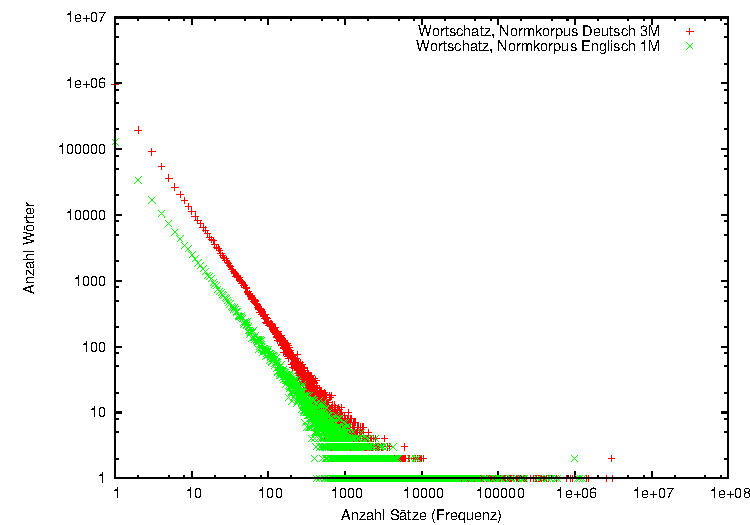
\includegraphics[width=\textwidth]{img/pdf/powerlaw_wortschatz.pdf}
%\caption{}
\label{fig:powerlaw_wortschatz}
\end{figure}

\begin{figure}[htb]
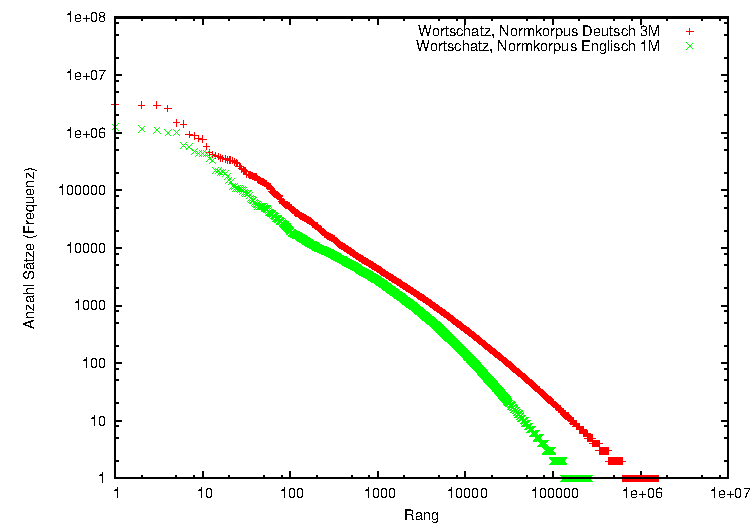
\includegraphics[width=1\textwidth]{img/pdf/zipf_wortschatz_reduced.pdf}
\caption[]{Frequenzverteilung in zwei ausgewählten Korpora}
\label{fig:zipf_wortschatz}
\end{figure}

\begin{figure}[htb]
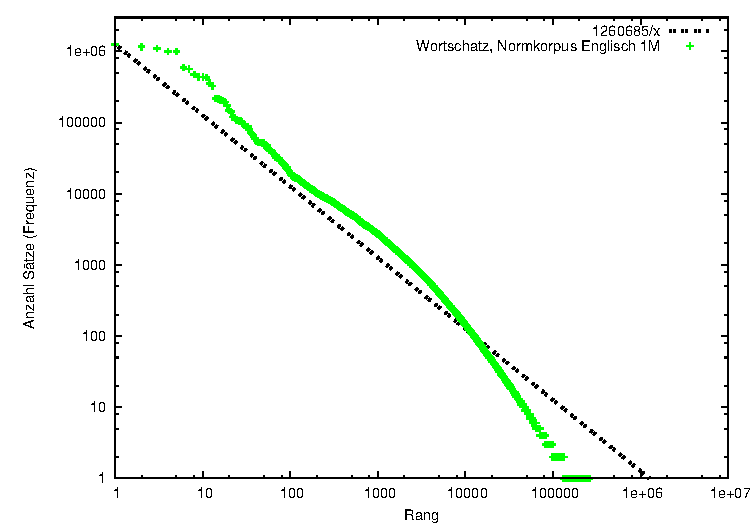
\includegraphics[width=1\textwidth]{img/pdf/zipf_wortschatz_with_expected_values_reduced.pdf}
\caption[]{Vergleich mit einer idealen Verteilung nach dem Zipfschen Gesetz}% $\frac{f_{\max}}{Rang}$
\label{fig:zipf_wortschatz_with_expected_values}
\end{figure}

\begin{figure}[htb]
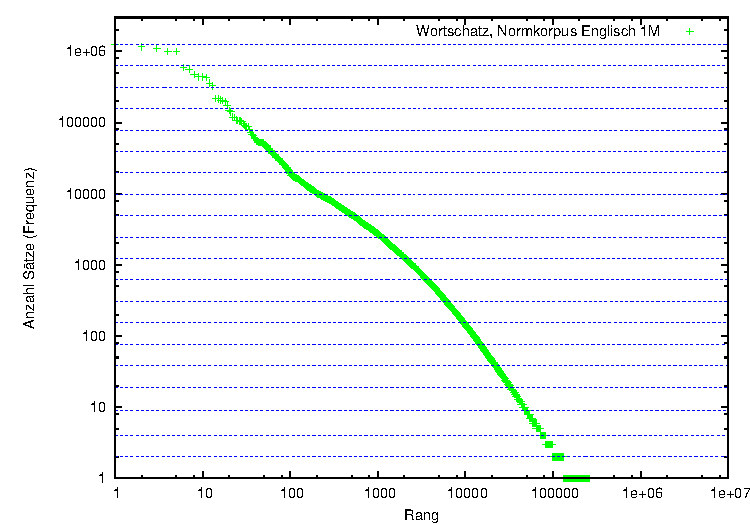
\includegraphics[width=1\textwidth]{img/pdf/zipf_wortschatz_frequency_class_reduced.pdf}
\caption[]{Aufteilung der Wortformen auf die verschiedenen Frequenzklassen}
\label{fig:zipf_wortschatz_frequency}
\end{figure}
\paragraph{} 
Die Daten des Wortschatzprojektes sind sowohl über ein Webportal\footnote{\url{http://corpora.informatik.uni-leipzig.de/}},
als auch per Download\footnote{\url{http://corpora.informatik.uni-leipzig.de/download.html}}
und als Webservice\footnote{\url{http://wortschatz.uni-leipzig.de/Webservices/}} verfügbar.

% dipl arbeit von christian biemann
% Seit 1994 wurde an der Universität Leipzig unter der Leitung von Uwe
% Quasthoff eine Infrastruktur erstellt, um elektronische Korpora zu
% analysieren und mit ihnen arbeiten zu können.
% Das inzwischen angesammelte Datenmaterial macht das :RUWVFKDW]-
% Korpus zu einem der größten Korpora in Deutsch, Englisch und
% Italienisch (je über 9 Mio. Sätze), desweiteren existieren noch kleinere
% Korpora in Französisch, Niederländisch und Sorbisch, sowie Korpora
% eingeschränkter Sachgebiete.
% Ziel bei der Erstellung war es, eine umfassende Datenbasis zu schaffen,
% um weitere Untersuchungen zu erleichtern. Die verarbeiteten Texte
% bestehen hauptsächlich aus einer Auswahl verschiedener Tageszeitungen,
% sowie Nachschlagewerken und von Verlagen für das Projekt freigegebenen
% Texten. Aus urheberrechtlichen Gründen dürfen die Texte nur satzweise
% gespeichert werden, weswegen der Satz die größte Einheit im Wortschatz
% darstellt.
% Auf die Rohdaten gestützt existieren verschiedene Datenbanken, die zur
% Strukturierung und als Vorarbeit für linguistische Algorithmen erstellt
% wurden. Als Vertreter seien hier die Kollokationsdatenbank, in der
%                                     -7-
% -
% Wortpaare,     die   signifikant  häufig    miteinander    in   Sätzen   oder
% nebeneinander auftreten, und die Datenbanktabelle 6DHW]H, die für alle
% indizierten Wörter Beispielsätze liefert, genannt.
% Im Gegensatz zum traditionellen Lexikon stellt die Wortschatz-Datenbank
% ein Vollformenlexikon dar, was sich aus der Konstruktion durch
% automatischen Aufbau ergibt. Hier gelten verschiedene Zeichenketten als
% verschiedene Wörter.
% Zum Datenbestand des deutschen Hauptkorpus gehören über 6 Millionen
% Wortformen,       über    36    Millionen    Sätze,   über    2,5   Millionen
% Grammatikangaben        sowie    Angaben     zur   Pragmatik,   Morphologie,
% Sachgebieten und weiteren Worteigenschaften.
% In einem Eintrag stehen die absolute Häufigkeit im Gesamtkorpus,
% Synonyme, Antonyme, Grammatikangaben, Sachgebiete, Beispielsätze und
% weiteres (siehe [Quasthoff 1998], [Quasthoff 2002a]).
% Der Wortschatz stellt einen Korpus im linguistischen Sinne dar: Bei der
% Auswahl der Texte wurde auf Vielfalt von Quellen und Sachgebieten
% geachtet, das Hauptkorpus wächst nicht weiter, liegt in maschinenlesbarer
% Form vor und ist mit eingeschränkten Suchmöglichkeiten im Internet seit
% März 1998 frei verfügbar.
\FloatBarrier

%\section{Ontology Learning}

%\section{Disambiguierung}
%\paragraph{Ähnlichkeitsmaß}\todo{...}
%Es handelt sich bei dieser Hierarchie um einen Baum

% %\chapter{State of the Art}
% \iffalse
% \section{Parser}
% Ein Parser für natürliche Sprachen ist ein Programm, welches die grammatikalische Struktur von Sätzen bestimmt und damit einen Syntaxbaum erstellt.
% In dieser Arbeit behandeln wir probabilistische Parser. Diese lernen die Struktur einer Sprache anhand von handannotierten Beispielen (einer Treebank) und
% erstellen dann bei Eingabe eines Satzes die Satzstruktur mit der höchsten Wahrscheinlichkeit. Auch wenn diese Art Parser noch ab und zu Fehler macht, funktionieren sie in der Praxis in den meisten Fällen sehr gut
% 
% \subsection{PCFG}
% A stochastic context-free grammar (SCFG; also probabilistic context-free grammar, PCFG) is a context-free grammar in which each production is augmented with a probability.
% The probability of a derivation (parse) is then the product of the probabilities of the productions used in that derivation;
% thus some derivations are more consistent with the stochastic grammar than others. SCFGs extend context-free grammars in the same way that hidden Markov models extend regular grammars.
% SCFGs have application in areas as diverse as Natural language processing to the study of RNA molecules. SCFGs are a specialized form of weighted context-free grammars.
% 
% Ein grundlegendes Problem der Lerntheorie ist, dass man theoretisch eine Sprache nicht nur aufgrund einer Menge positiver Beispiele (\zb{} einer Treebank) lernen kann.
% Wie Gold 1967 bewies\cite{gold67limit}, benötigen kontextfreie Grammatiken (und sogar schon Reguläre) zum Lernen sowohl positive als auch negative Beispiele.
% 
% Probabilistische kontextfreie Grammatiken können jedoch auch ausschließlich anhand von positiven Beispielen gelernt werden und erzielen in der Praxis damit sehr gute Ergebnisse.
% 
% Eine PCFG (probabilistische kontextfreie Grammatik) ist eine kontextfreie Grammatik, bei der jede Produktionsregel mit einer Wahrscheinlichkeit ausgezeichnet ist.
% Die Wahrscheinlichkeit einer Ableitung ist dann das Produkt der Wahrscheinlichkeiten der Produktionsregeln, die in der Ableitung vorkommen.
% Parst man nun einen Satz, der mehrere mögliche Ableitungen hat, dann kann man anhand der Wahrscheinlichkeiten dieser Ableitungen bestimmen, welcher dieser Syntaxbäume plausibler ist.
% Diese Plausibilitätseinschätzung ist allerdings nicht sehr gut, da sie nur auf der grammatischen Struktur des Satzes basiert und nicht darauf, welche Bedeutung des Satzes sinnvoller wäre.
% 
% 
% Laut\cite{accurate_unlexicalized_parsing} erreichten \todo{unlexicalized übersetzen} PCFG Parser im Test eine Genauigkeit von 86.36\% (LP/LR F1).
% 
% %\todo{übersetzt von \url{http://www.ps.uni-sb.de/~duchier/esslli-2000/node60.html#sec.dependency.formal}}
% \subsection{Phrasenstrukturgrammatik}
% Eine Phrasenstrukturgrammatik unterteilt einen Satz in eine hierarchische Gliederung aus sogenannten Phrasen oder Konstituenten.
% Sie ist sehr gut durch einen kontextfreie Grammatik repräsentierbar und \todo{was hierfür relevant ist}
% \todo{Bild}
% \subsection{Dependenzgrammatik}
% Eine Dependenzgrammatik (englisch Dependency Grammar) ist eine Grammatik, bei die Satzstruktur anhand von Abhängigkeiten von Wörtern untereinander dargestellt wird.
% Jedes Wort erzeugt eine bestimmte Zahl von Leerstellen im Text, es hat also eine bestimmte Valenz (Stelligkeit). Deshalb spricht man auch von einer Valenzgrammatik.
% Das zentrale Element eines Satzes in einer Dependenzgrammatik ist der sogenannte "`ultimative Head"', meist ein Verb.
% 
% Das Verb "`sehen"' etwa erwartet einen Sehenden und etwas Gesehenes.
% \begin{itemize}
%  \item "`Susi sieht die Sonne"' 
% \end{itemize}
% Andere Satzelemente kann man jedoch frei hinzufügen.
% \begin{itemize}
%  \item "`Susi sieht die Sonne, die heute sehr hell scheint."' 
% \end{itemize}
% \todo{Bild}
% 
% \paragraph{Vergleich}
% Hauptanliegen dieser Arbeit ist ja das Erlernen der charakteristischen Eigenschaften eines Satzes, um diesen gegen Andersartige abzugrenzen und Gemeinsamkeiten zu ähnlich Strukturierten zu finden.
% Da für jeden Grammatiktyp eine andere Ontologie erzeugt oder gefunden werden sowie ein Parser trainiert werden muss, ist es in dieser Arbeit aus Zeitgründen nicht möglich, beide zu integrieren und 
% hinsichtlich der Lernraten bei einigen häufigen Sprachfeatures zu analysieren. Aufgrund der modularen Struktur des Programmes ist es allerdings jederzeit nachrüstbar.
% Aus diesem Grund musste im Vorhinein eine Entscheidung gefällt werden, die zugunsten der Phrasenstrukturgrammatik ausfiel.
% Normalerweise werden Dependenzrepräsentationen für Sprachen mit großer Freiheit hinsichtlich der Wortreihenfolge (wie \zb{} Deutsch) empfohlen,
% Phrasenstrukturerepräsentationen werden hingegen für Sprachen mit festeren Satzstrukturen (wie \zb{} Englisch) vorgeschlagen.
% Trotzdem ist für beide Sprachen beides möglich. 
% \todo{Ist hier noch ein Beleg erforderlich? Wenn ja, dann Suchen und Einfügen, entnommen aus -> hier steht das drin http://www.ilc.cnr.it/EAGLES96/segsasg1/node44.html}
% 
% \begin{itemize}
%  \item 
%  \item Für das deutsche NEGRA Corpus existiert bereits eine Phrasenstrukturontologie 
%  \item Auch für das englische SUSANNE Corpus existiert bereits eine solche Ontologie
% \end{itemize}
% 
% 
% \cite{dependency_grammar_and_dependency_parsing} Dependency Grammar and Dependency Parsing
% 
% \iffalse
% Eine Dependancy Grammar ist ein 7-Tupel $<$Words, Cats, Args, Comps, Mods, Lexicon, Rules$>$.\\
% 
% \begin{tabular}{lp{12cm}}
% Words		&eine endliche Menge vollständig gebeugter Wörter\\
% Cats		&eine endliche Menge von Kategorien, \zb{} n (noun), det (determiner) oder vfin (finite verb)\\
% Args		&eine endliche Menge von "`agreement tuples"', \zb{} $<$masc sing 3 nom$>$\\
% Comps		&eine endliche Menge von "`complement roles"', \zb{} subject oder zu\_infinitive\\
% Mods		&eine endliche Menge von "`modifier roles roles"', \zb{} adj (adjective), welche disjunkt zu Comps ist. Wir schreiben $\textnormal{Roles} = \textnormal{Comps} \dotcup \textnormal{Mods}$.\\
% Lexicon		&eine endliche Menge von Lexikoneinträgen (siehe unten)\\
% Rules		&eine endliche Menge binärer Prädikate, indiziert mit den Rollenlabels $\varrho$, welche lokale grammatikalische Prinzipien ausdrücken. Für jedes $\varrho \in \textnormal{Roles}$ 
% gibt es ein $\Gamma_\rho \in \textnormal{Roles}$, sodass $\Gamma_\rho(w_1,w_2)$ anzeigt, ob eine Kante vom Vaterknoten $w_1$ zum Kindknoten $w_2$, die mit $\rho$ ausgezeichnet ist, existieren darf.\\
% \end{tabular}
% ~\\
% Ein lexikalischer Eintrag ist eine Wert-Attribut-Matrix mit der Signatur:
% 
% $
% \left[
% \begin{tabular}{cc}
% string	&Words\\
% cat	&Cats\\
% arg	&Agrs\\
% comps	&$2^\textnormal{Comps}$\\
% \end{tabular}
% \right]
% $\\
% Wenn $e$ ein Lexikoneintrag ist, dann ist string$(e)$ die vollständige Form des zugehörigen Wortes, cat$(e)$ dessen Kategorie, agr$(e)$ das agreement tuple und comps$(e)$ die Valenz ausgedrückt als 
% eine Menge von complement roles.
% 
% \subsubsection{Dependency Tree}
% Sei V eine Menge von Knoten, die wir mit den natürlichen Zahlen $\setN$ identifizieren.
% \fi
% 
% \iffalse
% \section{Disambiguierung}%\footnote{Im Englischen \emph{Word Sense Disambiguation}}
% Disambiguierung, im Englischen \emph{Word Sense Disambiguation}, beschäftigt sich damit, die Bedeutung eines Wortes in einem bestimmten Kontext herauszufinden.
% \begin{bsp}
% \emph{Hans setzte sich auf die Bank, denn die Sonne schien.}\\
% Welche Bedeutung hat das Wort \emph{Bank} in diesem Satz, ist hier das Möbelstück oder das Geldinstitut gemeint?
% \end{bsp}
% \subsection{Tiefer Ansatz}\todo{besser Übersetzen: deep approach}
% Dieser Ansatz setzt eine große Menge an Weltwissen vorraus. Hier könnte dies enthalten:
% "`Wenn die Sonne scheint, halten sich Menschen öfter in Parks auf. Parks enthalten oft Bänke (das Möbelstück). Auf eine Bank (das Möbelstück) kann sich ein Mensch setzen. Auf eine Bank (das Geldinstitut) kann sich ein
% Mensch nicht setzen"'.
% Das Problem bestand hier lange Zeit darin, dass außerhalb streng eingegrenzter Fachgebiete keine maschinenverarbeitbare Sammlung von Weltwissen verfügbar war.
% Es gab zwar Versuche, geschriebene Lexika maschinenlesbar aufzubereiten\cite{j:ewords}, dies brachte jedoch nur begrenzten Erfolg.
% Ein Quantensprung war dann jedoch das DBpedia-Projekt, das die riesige, sich ständig aktualisierende und erweiternde Wissensquelle Wikipedia automatisch zur Extraktion maschinenverarbeitbarer Daten nutzt.
% 
% These approaches are not very successful in practice, mainly because such a body of knowledge does not exist in a computer-readable format, outside of very limited domains. However, if such knowledge did exist, then deep approaches would be much more accurate than the shallow approaches.
% \fi
% \iffalse
% Deep approaches presume access to a comprehensive body of; world knowledge. Knowledge, such as "you can go fishing for a type of fish, but not for low frequency sounds"
%  and "songs have low frequency sounds as parts, but not types of fish", is then used to determine in which sense the word is used. These approaches are not very successful in practice, 
% mainly because such a body of knowledge does not exist in a computer-readable format, outside of very limited domains. However, if such knowledge did exist, then deep approaches would be 
% much more accurate than the shallow approaches. Also, there is a long tradition in computational linguistics, of trying such approaches in terms of coded knowledge and in some cases, it is
%  hard to say clearly whether the knowledge involved is linguistic or world knowledge. The first attempt was that by Margaret Masterman and her colleagues, at the Cambridge Language Research Unit in England,
% in the 1950s. This attempt used as data a punched-card version of Roget's Thesaurus and its numbered "heads", as an indicator of topics and looked for repetitions in text, using a set intersection algorithm.
%  It was not very successful, as is described in some detail in (Wilks, Y. et al., 1996), but had strong relationships to later work, especially Yarowsky's machine
%  learning optimisation of a thesaurus method in the 1990s.
% \fi\iffalse
% \subsection{Flache Ansätze}\todo{besser Übersetzen: shallow approach}
% \todo{material:}
% Preliminary Results in Tag Disambiguation using DBpedia
% 
% \cite{conf/naacl/Mihalcea07}
% \fi
% %\section{Ontology Learning}
% 
% %\section{Textklassifikation}
% \iffalse
% Rocchios Algorithmus
% 
% Rocchios Algorithmus basiert auf dem Relevanz-Feedback-Algorithmus.
% Er war einer der ersten RF-Algorithmen und wurde von J.J. Rocchio in \cite{rocchio_algorithm} vorgestellt.
% Relevanz-Feedback-Algorithmen sind eine effektive Möglichkeit, Benutzeranfragen zu erweitern oder zu verändern und daher \zb{} für Suchmaschinen sehr gut geegnet.
% Dabei wird die Anfrage schrittweise verfeinert, in dem aus allen als relevant oder irrelevant bekannten Dokumenten Merkmalsvektoren gebildet werden und aus diesen dann mit der folgenden Formel die nächste Anfrage
% berechnet wird:
% \[Q_j = \alpha Q_{j-1} + \frac{\beta}{N_R} \sum_{i=1}^{N_R} R_i + \frac{\gamma}{N_S} \sum_{i=1}^{N_S} S_i\]
% $Q_j$ ist dabei die Anfrage der Stufe $j$, $\alpha$, $\beta$ und $\gamma$ konstante Gewichtungen. $N_R$ ist die Anzahl relevanter, $N_S$ die Anzahl irrelevanter Dokumente. $(R_i)$ und $(S_i)$ sind die bereits
% als relevant bzw. irrelevant bestimmten Dokumente. $Q$, $R$ und $S$ sind dabei Vektoren von Termen aus einem Vektorraummodell. Aus dem resultierenden Anfragevektor werden sämtliche negativen Koeffizienten auf null gesetzt.
% Mit sämtlichen noch nicht eingestuften Dokumenten wird das Skalaprodukt zwischen dem Dokumentenvektor und dem Anfragevektor gebildet und nach dem Ergebnis ein Ranking gebildet, je höher das Skalarprodukt ist,
% desto höher die Relevanz des Ergebnisses. In einer Studie\cite{relevance_feedback_using_support_vector_machines} wird allerdings gezeigt, dass Rocchios Algorithmus schlecht abschneidet,
% wenn der Anteil relevanter Dokumente gering ist (wie es mittlerweile bei Spam der Fall ist,
% 
% \cite{a_hybrid_relevance-feedback_approach_to_text}
%                                             A recent study [3] revealed that
% Rocchio’s algorithm has a poor performance when the proportion of relevant
% documents in the whole corpus is quite low.
% \fi
% 
% \iffalse
% ****************BRIEF DESCRIPTION*********************
% 
% Rocchio’s Alogrithem
% 
% The Ricchio's Algorithm is based on the Relevancy Feedback Algorithms
% for Document Relevancy. Relevancy Feedback Models are an effective way
% of modifying and expanding user queries (such as search engines).
% 
% Ricchio's Algorithm is one of the earliest methods used for queries.
% This algorithm is basesd on the idea that if the relevance for a query
% is known, an optimal query vector will maximize the average
% query-document similarity for relevant documents, and will
% simultaneously minimize
% query-document similarity for non relevant documents. 
% 
% If we look at the basic formula for the Ricchio's Algorithm, the
% intuitive idea of Ricchio's Algorithm is to iteratively increase the
% weights of those terms contained in labeled relevant documents while
% penalizing the terms in the irrelevant documents.
% 
% Recent studies have shown that Ricchio's Algorithm has a poor
% performance when the proportion of relevant documents in the whole
% corpus is low.
% 
% http://www.cs.uml.edu/~kajal/courses/91.580-S03/papers/Hoashi.pdf
% http://www-student.cse.buffalo.edu/~arao/CSE741/slides.html
% http://ifsc.ualr.edu/xwxu/publications/ecir03_hybrid.pdf
% 
% 
% 
% 
% Naive Bayes
% 
% 
% 
% 
% Naive Byes algorithms are among the most successful known algorithms
% for learning to classify text documents. It predicts by reading a set
% of examples in attribute value-representation and than by using the
% Bayes Theorem to estimate the posterior probabilities of all
% qualifications. For each
% instance of the example language a classification with the highest
% posterier probability is chosen
% as the prediction. 
% 
% Example:
% 
% Suppose your data consist of fruits, described by their color and
% shape.  Bayesian classifiers operate by saying "If you see a fruit
% that is red and round, which type of fruit is it most likely to be,
% based on the observed data sample? In future, classify red and round
% fruit as that type of fruit."
% 
% A difficulty arises when you have more than a few variables and
% classes -- you would require an enormous number of observations
% (records) to estimate these probabilities.
% 
% Naive Bayes classification gets around this problem by not requiring
% that you have lots of observations for each possible combination of
% the variables.  Rather, the variables are assumed to be independent of
%  one another and, therefore the probability that a fruit that is red,
% round, firm, 3" in diameter, etc. will be an apple can be calculated
% from the independent probabilities that a fruit is red, that it is
% round, that it is firm, that is 3" in diameter, etc.
% 
% In other words, Naïve Bayes classifiers assume that the effect of an
% variable value on a given class is independent of the values of other
% variable. This assumption is called class conditional independence. It
% is made to simplify the computation and in this sense considered to be
% “Naïve”.
% 
% This assumption is a fairly strong assumption and is often not
% applicable.  However, bias in estimating probabilities often may not
% make a difference in practice -- it is the order of the probabilities,
% not their exact values, that determine the classifications.
% 
% Studies comparing classification algorithms have found the Naïve
% Bayesian classifier to be comparable in performance with
% classification trees and with neural network classifiers.  They have
% also exhibited high accuracy and speed when applied to large
% databases.
% 
% The problem with multinomial Naive Bayes is that when one class has
% more training examples than another, Naive Bayes selects poor weights
% for the decision boundary. This is due to an under-studied bias effect
% that shrinks weights for classes with few training examples. ANother
% systematic problem with Naive Bayes is that features are assumed to be
% independent. As a result, even when the words are dependent, each word
% contributes evidence individually. Thus the magnitude for the weights
% for classes with strong word dependencies is larger than for classes
% with weak word dependencies.
% 
% 
% http://www.wikipedia.org/wiki/Naive_Bayesian_classification
% http://www.dmg.org/pmmlspecs_v2/NaiveBayes.html
% http://www.cs.iastate.edu/~patterbj/cs/cs572/algs/naive.html
% http://www.resample.com/xlminer/help/NaiveBC/classiNB_intro.htm
% PORBLEMS WITH NAIVE BAYES
% http://www.ai.mit.edu/people/jrennie/papers/icml03-nb.pdf 
% 
% 
% 
% 
% K-Nearest Neighbor
% 
% 
% 
% 
% The goal of this clustering method is to simply separate the data
% based on the assumed similarities between various classes. Thus, the
% classes can be differentiated from one another by searching for
% similarities between the data provided.
% 
% The K-Nearest Neighbor is suitable for data streams. KNN does not
% build a classifier in advance. When a new sample arrives, KNN finds
% the K neighbors nearest to the new samples from the training space
% based on some suitable similarity or distance metric.
% 
% KNN is a good choice when simplicity and accuracy are the predominant
% issues. KNN can be superior when a  resident, trained and tested
% classifiers has a short useful lifespan, such as in the case with the
% data streams where new data is added rapidly and the training set is
% ever changing. KNN does not rely on prior probabilities, and it is
% computationally efficient. The main computation is the sorting of the
% training documents in order to find out the K nearest neighbors for
% the test document.
% 
% K-Nearest Neighbor is useful when their are less than 20 attributes
% per instance, there is lots of training data, training is very fast,
% learning complex target functions and don't want to loose information.
% The disadvantages of using such a function is that it is slow in
% sorting out queries and irrelevant attributes can fool the neighbor.
% 
% http://cs.hbg.psu.edu/~ding/publications/PAKDD02_KNN.pdf
% http://wwwcsif.cs.ucdavis.edu/~liaoy/research/text_ss02_html/node4.html
% http://www.cs.tufts.edu/~emower/KNN.html
% http://www4.cs.umanitoba.ca/~jacky/Teaching/Courses/74.436/current/Lectures/L07_Instance_Based_Learning.pdf
% 
% 
% 
% Decision Tree
% 
% 
% 
% The Decision Tree exploration engine, new to PolyAnalyst 4.1, helps
% solve the task of classifying cases into multiple categories. Decision
% Tree is PolyAnalyst's fastest algorithm when dealing with large
% amounts of  attributes. Decision Tree report provides an easily
% interpreted decision tree diagram and a predicted versus real table.
% 
% Problems to Solve: 
% 
% Classification of cases into multiple categories 
% 
% Target Attributes: 
% 
% Categorical or Boolean (Yes/No) attribute 
% 
% Output Format: 
% 
% Classification statistics 
% 
% Predicted versus Real table (confusion matrix) 
% 
% Decision Tree diagram 
% 
% Optimal Number of Records: 
% 
% Minimum of 100 records 
% 
% Maximum of 5,000,000 records 
% 
% Preprocessing Suggested: 
% 
% Summary Statistics - to deselect attributes that contain to many
% values to provide any useful insight to the exploration engine.
% 
% Underlying Algorithms: 
% 
% Information Gain splitting criteria 
% 
% Shannon information theory and statistical significance tests. 
% 
% The Data Used: 
% 
% Decision Tree works on data of any type. The DT algorithm is
% well-poised for analyzing very large databases  because it does not
% require loading all the data in machine main memory simultaneously.
% PolyAnalyst takes a  full advantage of this feature by implementing
% incremental DT learning with the help of the OLE DB for Data Mining
% mechanism.
% 
% The DT algorithm calculation time scales very well (grows only
% linearly) with increasing number of data columns. At the same time, it
% grows more than linearly with the growing number of data records - as
% N*log(N), where N is the number of records. Yet, for data of about
% 100,000 records, the DT algorithm is often the fastest exploration
% algorithm of PolyAnalyst.
% 
% Problems to Solve: 
% 
% Decision Tree algorithm helps solving the task of classifying cases
% into multiple categories. In many cases, this is the fastest, as well
% as easily interpreted machine learning algorithm of PolyAnalyst. The
% DT algorithm provides intuitive rules for solving a great variety of
% classification tasks ranging from predicting buyers/non-buyers in
% database marketing, to automatically diagnosing patient in medicine,
% and to determining customer attrition causes
% in banking and insurance. 
% 
% Target Attribute: 
% 
% The target attribute of a Decision Tree exploration must be of a
% Boolean (yes/no) or categorical data type.
% 
% When to Use This Algorithm: 
% 
% The Decision Tree exploration engine is used for task such as
% classifying records or predicting outcomes. You should use decision
% trees when you goal is to assign your records to a few broad
% categories. Decision Trees provide easily understood rules that can
% help you identify the best fields for further exploration.
% 
% The Output: 
% 
% The Decision Tree report starts of by giving measures resulting from
% the decision tree. These measures are the Number of non-terminal
% nodes, Number of leaves, and depth of the constructed tree. Next, the
% report provides classification statistics on the decision tree.
% 
% Problems:
% 
% The drawback of this algorithm is that large number of gini indices
% have to be computed at each node of the decision tree. In order to
% decide which attribute is to be split at each node, the gini indices
% have to be computed for all the attributes and for each successive
% pair of values for all patterns which have not been classified
% 
% OVERVIEW WITH AN EXAMPLE
% 
% http://www.bandmservices.com/DecisionTrees.htm
% 
% 
% 
% Support Vector Machine
% 
% 
% 
% A support vector machine is a supervised learning algorithm developed
% over the past decade by Vapnik and others (Vapnik, Statistical
% Learning Theory, 1998). The algorithm addresses the general problem of
% learning to discriminate between positive and negative members of a
% given class of n-dimensional vectors. For example, if you have a
% series of mRNA expression level measurements for each of a large
% number of genes, the SVM can learn to answer questions such as, ``Does
% the given gene belong to functional class X?'' where X is some
% category such as ``ribosomal genes'' or ``sugar and carbohydrate
% transporters.'' If you have a collection of digitized images of
% handwritten digits, the SVM can say whether a
% given image is, say, the number 9.
% 
% The SVM algorithm operates by mapping the given training set into a
% possibly high-dimensional feature space and attempting to locate in
% that space a plane that separates the positive from the negative
% examples. Having found such a plane, the SVM can then predict the
% classification of an unlabeled example by mapping it into the feature
% space and asking on which side of the separating plane the example
% lies. Much of the SVM's power comes from its criterion for selecting a
% separating plane when many candidates planes exist: the SVM chooses
% the plane that maintains a maximum margin from any point in the
% training set. Statistical learning theory suggests that, for some
% classes of well-behaved data, the choice of the maximum margin
% hyperplane will lead to maximal generalization when predicting the
% classification of previously unseen examples (Vapnik, Statistical
% Learning Theory, 1998). The SVM algorithm can also be extended to cope
% with noise in the training set and with multiple classes (Cristianini
% and Shawe-Taylor, An Introduction to Support Vector Machines, 2000).
% 
% Say that we have a training data set containing n examples, each of
% which is a vector of m numbers. These vectors may be thought of as
% points in an m-dimensional space. In theory, a simple way to build a
% binary classifier is to construct a hyperplane (i.e., a plane in a
% space with more than three dimensions) separating class members
% (positive examples) from non-members (negative examples) in this
% space. Unfortunately, most real-world problems involve non-separable
% data for which there does not exist a hyperplane that successfully
% separates the positive from the negative examples. One solution to the
% inseparability problem is to map the data into a higher-dimensional
% space and define a separating hyperplane there. This
% higher-dimensional space is called the feature space, as opposed to
% the input space occupied by the training examples. With an
% appropriately chosen feature space of sufficient dimensionality, any
% consistent training set can be made separable. However, translating
% the training set into a higher-dimensional space incurs both
% computational and learning-theoretic costs. Furthermore, artificially
% separating the data in this way exposes the learning system to the
% risk of finding trivial solutions that overfit the data.
% 
% SVMs elegantly sidestep both difficulties. They avoid overfitting by
% choosing the maximum margin separating hyperplane from among the many
% that can separate the positive from negative examples in the feature
% space. Also, the decision function for classifying points with respect
% to the hyperplane only involves dot products between points in the
% feature space. Because the algorithm that finds a separating
% hyperplane in the feature space can be stated entirely in terms of
% vectors in the input space and dot products in the feature space, a
% support vector machine can locate the hyperplane without ever
% representing the space explicitly, simply by defining a function,
% called a kernel function, that plays the role of the dot product in
% the feature space. This technique avoids the computational burden of
% explicitly representing the feature vectors.
% 
% http://www-ai.cs.uni-dortmund.de/SOFTWARE/SVM_LIGHT/svm_light_v3.02.eng.html
% http://www.afia.polytechnique.fr/CAFE/ECML01/SVM.html
% 
% 
% 
% Latent Semantic Analysis
% 
% 
% 
% Latent Semantic Analysis (LSA) analyzes word-word, word-passage, and
% passage-passage relationships. There's a good relationship between
% what LSA extracts and what people understand. LSA doesn't use
% first-hand knowledge of the world, but extracts from "episodes" of
% word content. LSA doesn't use word order or logic relationships. LSA
% uses unitary expressions of meaning instead of relationships between
% successive words. A word is a kind of average of meaning through all
% passages.
% 
% Dimensionality is reduced to approximate human cognition. LSA is a
% theory of knowledge representation. Dimensionality reduction solves
% the problem of "insufficient evidence" or "poverty of the stimulus".
% LSA uses a matrix decomposition algorithm to reduce the
% dimensionality. Ideally, the dimension of the reconstruction equals
% that of the passages. Results show that the meaning similarities are
% close to that of humans, LSA's rate of knowledge acquisition
% approximates that of humans, and LSA depends on the dimensionality.
% 
% LSA can be use to test theories of human cognition. LSA skips over the
% order of words to capture relationships in word choice. LSA uses a
% pre-processing step for word correlation over many passages and
% contexts. LSA uses a very large number of relationships. Theories of
% human cognition cannot be settled by theoretical and philosophical
% ideas.
% 
% LSA is an automatic mathematical algorithm for extracting
% relationships in word usage in passages. It doesn't use dictionaries,
% external knowledge, or grammar rules. First, represent words as a
% matrix, each row is a word, and each column is a text passage or
% context. Next, do a preliminary transformation of the matrix. Each
% word frequency in the Next, LSA applies singular value decomposition
% (SVD) to the matrix, which is factor analysis. The decomposition
% results in dimensionality reduction. Extract words from the passage
% into a word matrix, do a linear decomposition of the matrix, then
% reduce the dimensionality of the matrix. The LSA matrix adds words not
% in the passage, like human minor knowledge acquisition. LSA is
% intuitively sensible, with a three-fourths gain in total comprehension
% vocabulary inferred from knowledge about words not in the passage or
% paragraph. Human children have a rapid growth of vocabulary and
% knowledge. Humans draw conclusions from missing data. Reducing the
% dimensionality of representation is useful when the representation
% matches the data. The data should not be perfectly regenerated. The
% similarity of dimensionality reduction is the cosine between vectors.
% 
% Before the SVD is computed, LSA does a data preprocessing matrix data
% transformation. Save the log word frequency, and the entropy for each
% row and column of the word. Weight each word occurrence by an estimate
% of its importance in the passage. Knowing a word provides information
% about the passage it appeared in. Matrix transformations are used in
% information retrieval and human cognition models. A web site provides
% LSA based word or passage vectors, similarities between words and
% words, words and passages, and passages and passages. LSA is able to
% model human conceptual knowledge.
% LSA links information retrieval and human semantic memory. Latent
% Semantic Indexing (LSI), like LSA, was tested against pre-examined
% documents. Direct comparisons were muddied by preprocessing words. LSA
% does synonym tests, since most near neighbors are related by the
% cosine. LSA vectors were created from many passages. LSA captures
% synonymity by knowledge
% of captured vocabularies. TOEFL vocabulary simulates human performance
% between word choice. LSA errors were compared to student errors. The
% role of dimension reduction was analyzed. LSA simulates word sorting
% and word relationships. Subject-matter knowledge and sematic priming
% are in LSA. Predictive learning and text comprehension for humans.
% 
% http://www.uni-koblenz.de/~fruit/publications/Obst99c.html
% http://www.cs.toronto.edu/~psy/lsa.pdf 
% http://www.cs.nmsu.edu/~mmartin/LSA_Intro_AI_Seminar.ppt
% 
% RESOURCE
% 
% http://citeseer.nj.nec.com/563891.html
% 
% Voted Classification
% 
% http://216.239.39.104/search?q=cache:CcXO0h6c-Z4J:robotics.stanford.edu/users/ronnyk/vote.pdf+voted+classification+algorithm&hl=en&ie=UTF-8
% \fi
%\section{Modul \textit{Domänenidentifizierung}}
\begin{center}
\begin{tabular}{l|l}
\multicolumn{2}{c}{Modulabhängigkeiten}\\
Vorraussetzung& Empfohlen\\
\hline
\textit{Wortschatz2DBpedia} & \textit{Disambiguation}
\end{tabular}

\end{center}

\subsection{Problemstellung}
Eine wichtiges Merkmal höherer Ordnung\todo{klingt das ok?} eines Textes, das zu seiner Klassifizierung beitragen kann, ist die Domäne, also der Gegenstand oder auch Fachgebiet des Textes.
Um zu einer große Menge von Texten eine passende Domäne zur Verfügung zu haben und um aus den im Text vorhandenen Konzepten auf einen gemeinsamen Gegenstand zu schließen, wird eine
umfangreiche taxonomische (Superklassen-) Hierarchie benötigt.
\todo{den ganzen satz vielleicht zum wortschatz2dbpedia-modul schieben} Durch das NLP2RDF-Modul \textit{Wortschatz2DBpedia} werden zu den im Text vorkommenden, explizit angegebenen Substantive\footnotemark 
\footnotetext{Da zum Zeitpunkt der Diplomarbeit keine Anapher-Resolution verfügbar ist, können indirekt angegebene Substantive ("`\textit{Der Präsident von Norwegen} bekam den Friedensnobelpreis."',
"`\textit{Er} bestellte noch einen Kaffee."' nicht aufgelöst - und damit auch nicht klassifiziert - werden.}
Referenzen zu den Wikipedia-Artikeln hinzugefügt, 
\subsection{YAGO}
\textit{YAGO}\cite{yago} ist eine große Ontologie von Weltwissen mit hoher Präzision und Coverage, die automatisch aus Wikipedia und WordNet erstellt wurde.
YAGO zeichnet sich dadurch aus, dass es die exzellente, von Hand gepflegte, Taxonomie von Wordnet mit der Vielfalt von Artikeln und damit Konzepten aus Wikipedia verbindet.

Zu jedem Wikipedia-Artikel enthält YAGO ein passendes Individuum. Dabei ist jeder Wikipedia-Artikeltitel ein Kandidat, ein YAGO-Individuum zu werden.

\begin{bsp}
"`The Enterprise is in space."'
Durch Ausführung von Wortschatz2DBpedia und einer Disambiguierung haben wir beispielhaft die referenzierten Wikipedia-Artikel \url{Starship_Enterprise} und \url{Outer_Space} extrahiert.
\begin{center}
\begin{tabular}{llll}
Wort		&Artikelname			&YAGO-Individuum\\
\hline
Enterprise	&\url{Starship_Enterprise}	&\url{Starship} \url{Enterprise}\\
space		&\url{Outer_Space}		&\url{outer} \url{space}\\
\end{tabular}

\begin{tabular}{llll}
YAGO-Individuum			&type			&subClassOf\\
\hline
\url{Starship} \url{Enterprise}	&Star Trek ships	&~\\
~				&craft			&~\\
~				&\ldots			&~\\
\url{outer} \url{space}		&~			&space\\
~				&~			&location\\
\end{tabular}
\end{center}


\end{bsp}

\todo{Describes-Relation einbauen}


Der Wikipedia-Seitentitel "`Starship Enterprise"' ist also ein Kandidat, das Individuum \url{Starship} \url{Enterprise} in YAGO zu werden.


Wir erhalten also aus einer Menge von Artikeln eine Menge von Individuen.
Für jedes dieser Individuen interessieren uns nun die zugehörige Klassen in der Hierarchie von YAGO.
Die Subklassenhierarchie wird in YAGO durch die Relation \textit{TYPE} ausgedrückt.

\url{Elephant} TYPE \url{Elephants}

Die YAGO-Klassenhierarchie hat die Gestalt eines \textit{DAG}s (directed acyclic graph, gerichteter azyklischer Graph)

%Mit Hilfe der \textit{YAGO}-Klassenhierarchie wird eine 

Durch die Ausführung von Wortschatz2DBpedia ist jedes Wort mit einer Menge an möglichen passenden Wikipedia-Artikeln ausgezeichnet. Wurde zusätzlich noch eine Disambiguation ausgeführt, dann ist dies für 
jedes Wort genau ein passender Wikipedia-Artikel.


\subsection{Extrahieren der YAGO-Klasse und der Klassenhierarchie}
Das Modell der YAGO-Ontologie\footnote{Download unter \url{http://www.mpi-inf.mpg.de/yago-naga/yago/yago.zip} (1 Gb)} benutzt dieselbe Wissensrepräsentation wie RDFS.
die 

Die Klassenhierarchie findet sich unter \url{facts/subClassOf/WordNetLinks.txt}.

Die Zuordnung von Wikipedia-Klassen zu Wordnet-Klassen findet sich unter \url{facts/subClassOf/ConceptLinker.txt}.
Durch Sortieren nach der Wordnet-Klasse lässt sich durch binäre Suche die Performance wesentlich erhöhen.

\url{facts/type/IsAExtractor.txt}
\include{state_of_the_art}
\chapter{NLP2RDF}

\emph{NLP2RDF}\footnote{Webseite \url{http://nlp2rdf.org}, Download (Open Source) unter \url{http://code.google.com/p/nlp2rdf}}
ist ein Framework, das viele verschiedene Tools zur Verarbeitung natürlicher Sprache (\emph{natural-language processing, NLP}) integriert.
NLP2RDF verarbeitet geschriebene Sätze und wandelt diese in eine RDF-Struktur um, die mit syntaktischen und semantischen Zusatzinformationen angereichert ist.
\begin{figure}[htb]
\begin{center}
\begin{threeparttable}
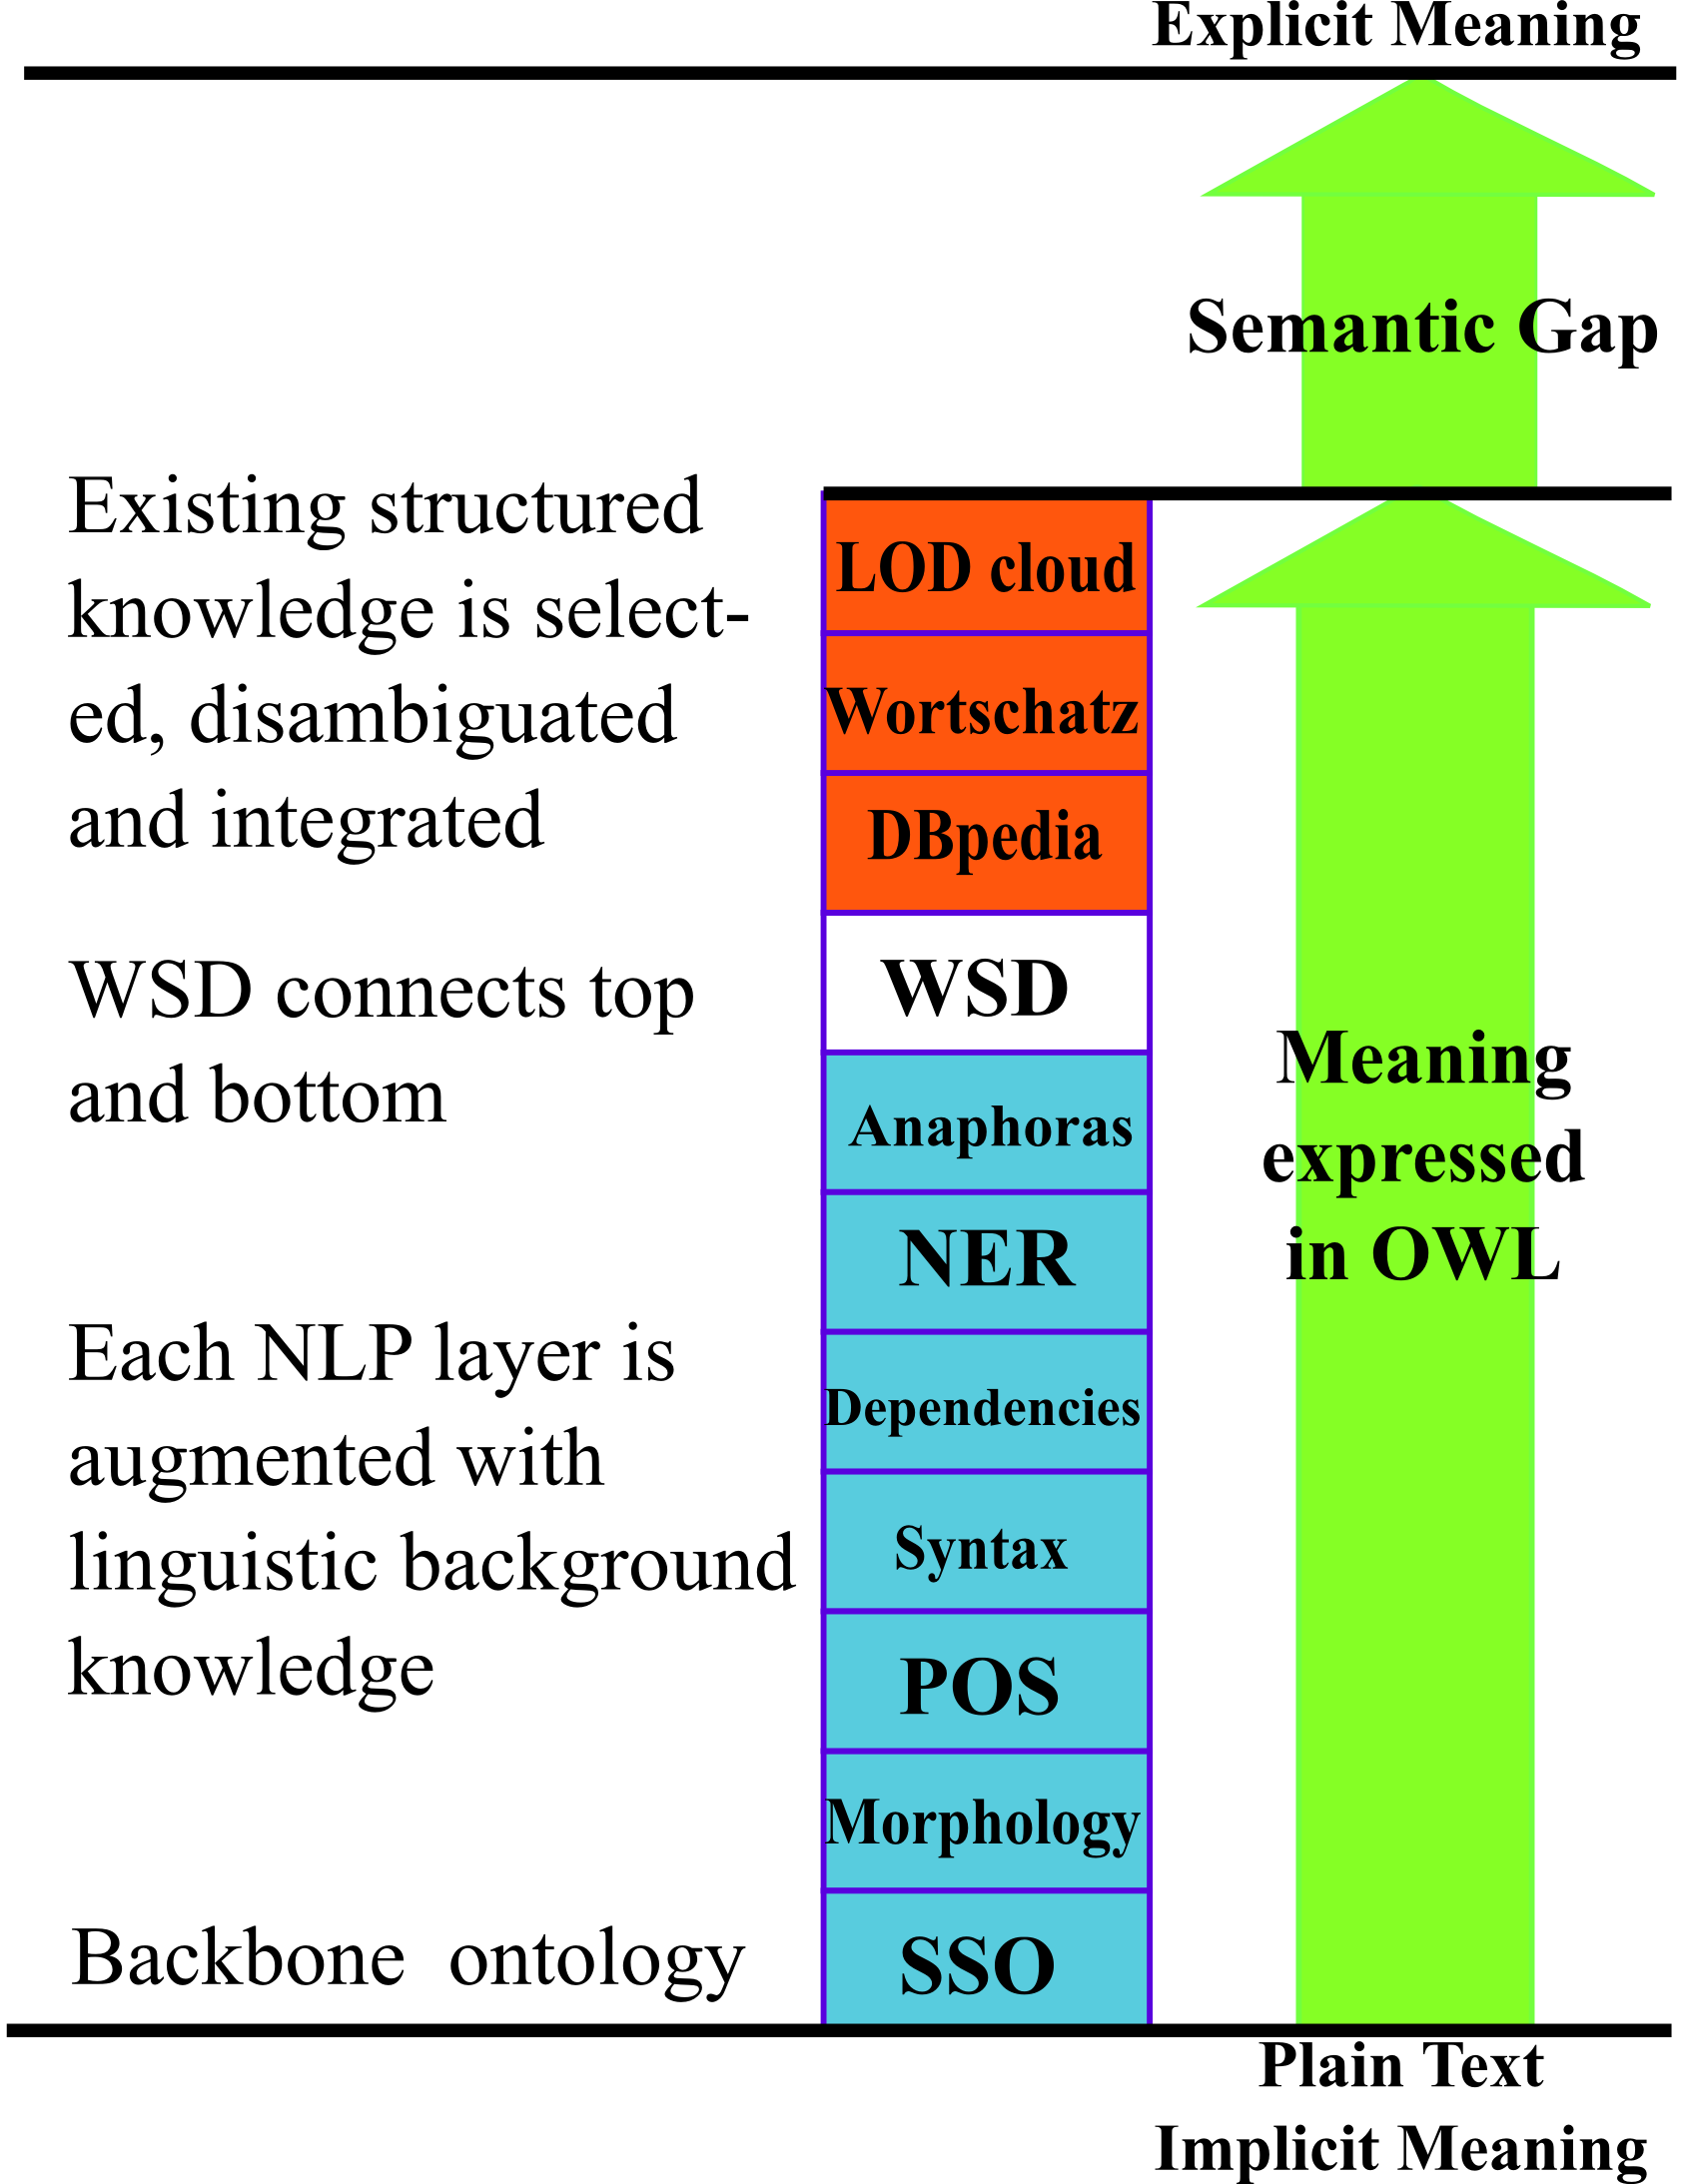
\includegraphics[width=0.5\textwidth]{img/nlp2rdf_stack.png}
\begin{tablenotes}\footnotesize
 \item [] Quelle: \citet{tiger_corpus_navigator}
\end{tablenotes}
\end{threeparttable}
\caption{Der \emph{NLP2RDF stack}}
\label{fig:nlp2rdf_stack}
\end{center}
\end{figure}
Dabei werden die Sätze zunächst durch einen Chunker in Tokens zerlegt, aus denen ein Grundgerüst erstellt wird, die \emph{Structured Sentence ontology (SSO)}.
Die SSO besteht nur aus einem minimalen Vokabular und der grundlegenden Struktur des Satzes in Form der Tokens und ihrer Position im Satz, siehe Abbildung \ref{fig:nlp2rdf_sso}.
Nun werden schrittweise Zusatzinformationen hinzugefügt.
Im ersten Schritt sind dies Features aus NLP-Verfahren (türkis bzw. hellgrau in Abbildung \ref{fig:nlp2rdf_stack}), im zweiten Schritt Ontologien für diese Features.
Dem Wort "`wir"' eines Satzes könnte also im ersten Schritt das Feature "`ist ein Personalpronomen"' zugeordnet werden und dem Wort "`unser"' eines anderen Satzes das Feature "`ist ein Possessivpronomen"'.
Enthält nun die Ontologie die Klassenbeziehungen "`ein Personalpronomen ist ein Pronomen"' und "`ein Personalpronomen ist ein Pronomen"', dann macht dies die Aussage
"`beide Sätze enthalten ein Pronomen"' möglich, was wiederum weitere Schlussfolgerungen auf komplexere Features ermöglicht.
Im dritten Schritt wird nun eine \emph{Wortsinndisambiguierung} (im Folgenden auch nur \emph{Disambiguierung} oder \emph{WSD}, eine Mehrdeutigkeitsauflösung) durchgeführt und Hintergrundwissen aus dem Semantischen Web (rot bzw. dunkelgrau) hinzugefügt.
Im Satz "`Er war ein echter Berliner und fühlte sich in seiner Stadt pudelwohl."' würde beispielsweise die Disambiguierung festlegen, dass sich das Wort "`Berliner"' nicht auf den \emph{Berliner Pfannkuchen} sondern auf
die Stadt \emph{Berlin} bezieht, worauf nun weitere Informationen über diese Stadt in die Struktur integriert werden könnten, \zb{} die Einwohnerzahl und geographische Lage der Stadt Berlin.
%Im Satz "`Er kaufte sich einen Pfannkuchen mit einer Füllung aus Konfitüre"' 

%\paragraph{Ein Beispiel}

\begin{figure}
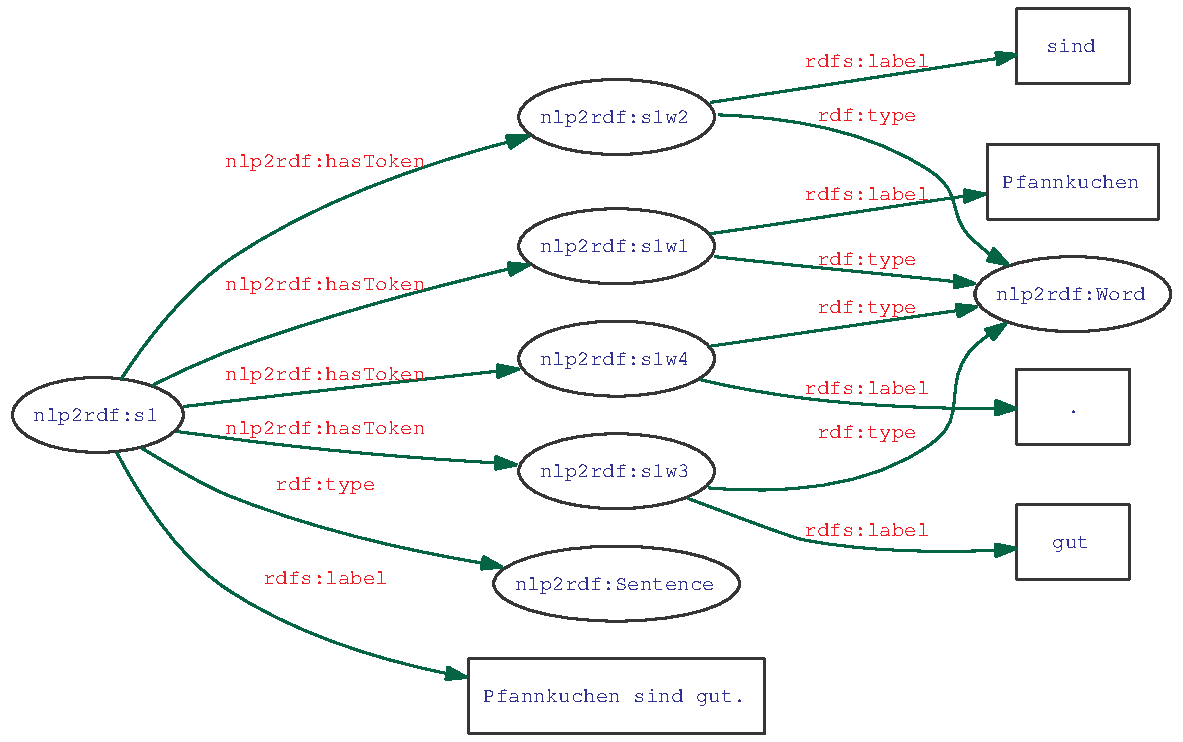
\includegraphics[width=\textwidth]{img/pdf/sso.pdf}
\caption{die \emph{Sentence Structure ontology} eines Beispielsatzes}
\label{fig:nlp2rdf_sso}
\end{figure}
%\footnote{\url{http://www.w3.org/RDF/Validator/}}
\iffalse
\lstset{language=XML}
\begin{lstlisting}
<?xml version="1.0"?>
<rdf:RDF xmlns:rdf="http://www.w3.org/1999/02/22-rdf-syntax-ns#"
    xmlns="http://nlp2rdf.org/"
    xmlns:ns0="http://www.w3.org/2002/07/owl#"
    xmlns:dcterms="http://purl.org/dc/terms/"
    xmlns:xsd="http://www.w3.org/2001/XMLSchema#"
    xmlns:j.0="http://141.89.100.105/owl/stts.owl#"
    xmlns:j.1="http://www.w3.org/2000/01/rdf-schema#" > 
 
  <rdf:Description rdf:about="http://nlp2rdf.org/s1">
    <hasWord rdf:resource="http://nlp2rdf.org/s1w1"/>
    <hasWord rdf:resource="http://nlp2rdf.org/s1w2"/>
    <hasWord rdf:resource="http://nlp2rdf.org/s1w3"/>
    <hasWord rdf:resource="http://nlp2rdf.org/s1w4"/>
    <rdf:type rdf:resource="http://nlp2rdf.org/Sentence"/>
    <j.1:label>Pfannkuchen sind gut.</j.1:label>
  </rdf:Description>
 <rdf:Description rdf:about="http://nlp2rdf.org/s1w1">
    <j.1:label>Pfannkuchen</j.1:label>
    <rdf:type rdf:resource="http://nlp2rdf.org/Word"/>
  </rdf:Description>
 <rdf:Description rdf:about="http://nlp2rdf.org/s1w2">
    <j.1:label>sind</j.1:label>
    <rdf:type rdf:resource="http://nlp2rdf.org/Word"/>
  </rdf:Description>
 <rdf:Description rdf:about="http://nlp2rdf.org/s1w3">
    <j.1:label>gut</j.1:label>
    <rdf:type rdf:resource="http://nlp2rdf.org/Word"/>
  </rdf:Description>
 <rdf:Description rdf:about="http://nlp2rdf.org/s1w4">
    <j.1:label>.</j.1:label>
    <rdf:type rdf:resource="http://nlp2rdf.org/Word"/>
  </rdf:Description>
</rdf:RDF>
\end{lstlisting}
\lstset{language=Java}
\fi
\iffalse
das hier für die visualisierung benutzen (rdf:x durch rdf1:x ersetzen), damit die abkürzungen reinkommen statt der vollen uri
    <?xml version="1.0"?>
<rdf:RDF
    xmlns:rdf="http://www.w3.org/1999/02/22-rdf-syntax-ns#"
    xmlns:rdf1="rdf:"
    xmlns:nlp2rdf="nlp2rdf:"
    xmlns="nlp2rdf:"
    xmlns:ns0="owl:"
    xmlns:dcterms="dcterms:"
    xmlns:xsd="xsd:"
    xmlns:j.0="stts:"
    xmlns:j.1="rdfs:" > 
 
  <rdf:Description rdf:about="nlp2rdf:s1">
    <hasToken rdf:resource="nlp2rdf:s1w1"/>
    <hasToken rdf:resource="nlp2rdf:s1w2"/>
    <hasToken rdf:resource="nlp2rdf:s1w3"/>
    <hasToken rdf:resource="nlp2rdf:s1w4"/>
    <rdf1:type rdf:resource="nlp2rdf:Sentence"/>
    <j.1:label>Pfannkuchen sind gut.</j.1:label>
  </rdf:Description>
 <rdf:Description rdf:about="nlp2rdf:s1w1">
    <j.1:label>Pfannkuchen</j.1:label>
    <rdf1:type rdf:resource="nlp2rdf:Word"/>
  </rdf:Description>
 <rdf:Description rdf:about="nlp2rdf:s1w2">
    <j.1:label>sind</j.1:label>
    <rdf1:type rdf:resource="nlp2rdf:Word"/>
  </rdf:Description>
 <rdf:Description rdf:about="nlp2rdf:s1w3">
    <j.1:label>gut</j.1:label>
    <rdf1:type rdf:resource="nlp2rdf:Word"/>
  </rdf:Description>
 <rdf:Description rdf:about="nlp2rdf:s1w4">
    <j.1:label>.</j.1:label>
    <rdf1:type rdf:resource="nlp2rdf:Word"/>
  </rdf:Description>
</rdf:RDF>
\fi

\section{Der Parser}
Die Morphologie und die \emph{Part of Speech} (POS) \emph{Tags} eines Eingabesatzes werden von einem Parser bestimmt.
%Diese Struktur wird dann in RDF modelliert und wie ein Weihnachtsbaum von beliebigen weiteren Tools mit Zusatzinformationen behängt.

%\begin{floatingfigure}[r]{0.5\textwidth}
\begin{figure}[0.5\textwidth]
    %\centering
    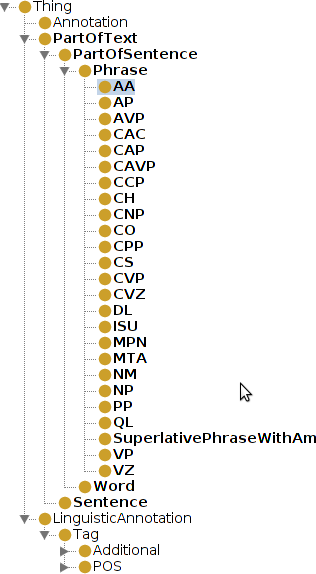
\includegraphics[width=0.5\textwidth]{img/stts_ontology_alpha.png}
    \caption{die angepasste STTS-Ontologie (frühe Version)}
    \label{fig:stts_ontology_alpha}
\end{figure}
%\end{floatingfigure}

Dabei wird der statistische Parser der Stanford Natural Language Group\footnote{\url{http://nlp.stanford.edu/software/lex-parser.shtml}} benutzt, aufgrund der modularen Struktur von NLP2RDF
sind andere Parser aber auch problemlos einbindbar.
Für nichtkommerzielle Nutzung ist er frei verfügbar und als Javaprogramm leicht integrierbar.
Ein trainiertes Modell ist unter anderem für Deutsch und Englisch bereits enthalten.

%Um den Output des Parsers in eine RDF-Struktur zu übertragen, ist eine passende Ontologie nötig, welche die Relation der Annotierungen untereinander festlegt (\zb{} "`Ein Reflexivpronomen ist ein Pronomen"').
Da der deutsche Parser\footnote{germanFactored.ser.gz} auf dem Negra Corpus\footnote{\url{http://www.coli.uni-saarland.de/projects/sfb378/negra-corpus/negra-corpus.html}} basiert,
 welches das Stuttgart-Tübingen Tagset (STTS)\footnote{\url{http://www.sfs.uni-tuebingen.de/Elwis/stts/stts.html}} benutzt,
kann eine bereits existierende STTS-Ontologie\footnote{\url{http://141.89.100.105/owl-docu/stts.html}} mit kleineren Erweiterungen direkt benutzt werden (siehe Abbildung \ref{fig:stts_ontology_alpha}).

Die mitgelieferten englischen Parser\footnote{englishFactored.ser.gz und englishPCFG.ser.gz} benutzen die Tags des Penn Treebank Projektes\footnote{\url{http://www.cis.upenn.edu/~treebank/}} -- das Penn Treebank Tag Set.
Eine passende Ontologie wird freundlicherweise von Herrn Christian Chiarcos\footnote{Arbeitsseite: \url{http://www.sfb632.uni-potsdam.de/~chiarcos/}} zur Verfügung gestellt.
Sie wurde im Rahmen des Projektes “Sustainability of Linguistic Data” an der Universität Potsdam entwickelt und gehört zu einem integrativen Framework \citep{ontology-based_interface_specifications}.

\iffalse
%
\iffalse
Unglücklicherweise konnte keine Ontologie für das Penn Treebank Tag Set gefunden werden. Aufgrund des bereits großen Umfanges dieser Arbeit und des Umstandes, das der Autor kein ausgebildeter Sprachwissenschaftler ist,
 erschien es auch nicht praktikabel, solch eine Ontologie selbst zu erstellen.
Das Umlernen eines POS-Taggers auf ein anderes Tagset ist beim Stanford Parser jedoch möglich, wenn man ihn mit POS-annotierten Trainingstexten versorgt.\footnote{\url{http://nlp.stanford.edu/software/parser-faq.shtml#f}}
Es war also nur noch eine beliebige für das Englische geeignete Ontologie gesucht, für die es POS-annotierten Text gibt.
Die Wahl fiel dabei auf das Susanne\footnote{Surface and underlying structural analysis of natural English}-Tagset.
Sowohl das Susanne Corpus, eine passende Treebank\footnote{\url{www.grsampson.net/Resources.html}} als auch die Ontologie\footnote{\url{http://141.89.100.105/owl-docu/susa.html}} sind frei verfügbar.

In der FAQ des Stanford Parsers wird ein Satz angegeben, der das erwartete Format deutlich macht:

\begin{verbatim}
`The/DT quick/JJ brown/JJ fox/NN jumped/VBD over/IN the/DT lazy/JJ dog/NN ./.
\end{verbatim}

Die Treebank besteht jedoch aus mehreren Dateien, welche Zeilen wie diese enhalten:
\begin{verbatim}
G12:0030.27	-	PPHS1m	He	he	[S[Nas:s.Nas:s]
G12:0030.30	-	VBDZ	was	be	[Vsu.
G12:0030.33	-	VVGv	waiting	wait	.Vsu]S]
G12:0030.39	-	YF	+.	-	.O]
\end{verbatim}
Das gewünschte Format kann daraus jedoch erzeugt werden.

Zusammenführen aller relevanten Dateien in Eine:
\begin{verbatim}
find | sed "s/\.\///" |
egrep -v "lexicon|documentation|\." |
xargs cat >>allinone.txt
\end{verbatim}
Auswählen der relevanten Spalten:
\begin{verbatim}
cat allinone.txt | cut -f3,4 > allinone_tag_and_word.csv
\end{verbatim}
Vertauschen der Spalten und Einsetzen des Trennzeichens:
\begin{verbatim}
cat allinone_tag_and_word.csv |
sed "s/\([^\t]*\)\t\([^\t]*\)/\2\/\1/"
> allinone_stanfordformat.txt
\end{verbatim}
Alle Zeilenumbrüche entfernen:
\begin{verbatim}
cat allinone_stanfordformat.txt |
tr "\n" " " > allinone_stanfordformat_oneline.txt
\end{verbatim}
Zeilenumbrüche nach dem Satzende hinzufügen um das endgültige Format zu bekommen:
\begin{verbatim}
cat allinone_stanfordformat_oneline.txt |
sed "s/+\.\/YF /+\.\/YF\\n/g"
> susanne_treebank_readyfortraining.txt
\end{verbatim}
\todo{was ist mit einem trainierten parser model für die susa.owl?}
\todo{was ist mit einem trainierten parser model für die susa.owl?}
\fi
Aufgabe ist die Featureerkennung geschriebener Sprache. Ein Feature ist eine beliebige Eigenschaft von Sprache.
Das Programm soll folgendes leisten:
\begin{itemize}
\item erlernen von Regeln für ein Feature einzig aufgrund angebener positiver (und optional auch negativer) Lernbeispiele
\item bestimmen, ob eine solche Regel auf einen gegebenen Satz zutrifft
\item bestimmen der Teilmenge einer Menge von Sätzen, auf die diese Regel zutrifft\footnote{}
\end{itemize}

\begin{bsp}
\begin{itemize}
\item Wie definiert man einen Aktivsatz?
\item Für meinen Unterricht benötige ich 10 kurze Beispielsätze mit Reflexivpronomen
\item Extrahiere mir aus diesem Text alle Sätze, die Personen beinhalten
\end{itemize}

\todo{Was es bereits gibt}

Müsste man das Rad neu erfinden, wäre das wohl eine für eine Diplomarbeit unlösbare Aufgabe.
Zum Glück existieren jedoch bereits 
- 
\end{bsp}


Die Penn Treebank hat das folgende Format für Bäume:
Hier ist das teilweise beschrieben:
\url{http://search.cpan.org/~kahn/Lingua-Treebank-0.14/Treebank.pm#___top}
\fi

\section{Der TIGER Corpus Navigator}\label{sec:tiger_corpus_navigator}

\begin{figure}[htb]
\begin{center}
\begin{threeparttable}
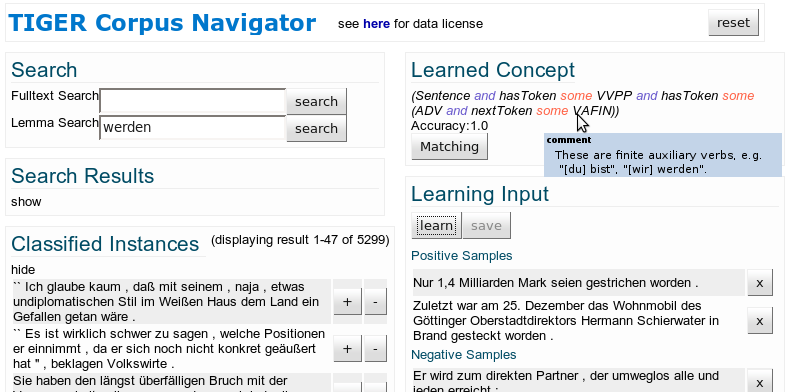
\includegraphics[width=\textwidth]{img/tigercorpusnavigator_screenshot.png}
\begin{tablenotes}\footnotesize
 \item [] Quelle: \citet{tiger_corpus_navigator}
\end{tablenotes}
\end{threeparttable}
\caption{die Benutzeroberfläche auf \url{http://tigernavigator.nlp2rdf.org}}
\label{fig:tigercorpusnavigator_screenshot}
\end{center}
\end{figure}

%Obwohl eine große Menge annotierter Corpora verfügbar ist, stellt das Abrufen von daraus ableitbarem Wissen immer noch ein Problem dar.
Eine erste Anwendung des NLP2RDF-Frameworks ist der \emph{TIGER Corpus Navigator} von \citet*{tiger_corpus_navigator},
mit dem ein Benutzer Sätze aus dem \emph{TIGER Corpus} \citep{tiger1,tiger2} abrufen und klassifizieren kann.
Der TIGER Corpus Navigator verwendet Algorithmen des maschinellen Lernens und erlaubt es, formale Definitionen aus benutzerdefinierten Konzepten zu erlernen.
Ein Konzept wird definiert, indem der Benutzer mithilfe einer Volltext- oder Lemmasuche eine Untermenge des Corpus bestimmt und aus dieser positive und negative Beispiele auswählt (siehe Abbildung \ref{fig:tigercorpusnavigator_screenshot}).
Das Programm generiert aus diesen Beispielen eine formale OWL-Klassendefinition, die der Benutzer durch die Angabe von weiteren Beispielen noch verfeinern kann.
Dieses Verfahren ist jedoch nicht ohne weiteres möglich, da für einen generischen Lernalgorithmus Texte nur eine Menge unstrukturierter Informationen darstellen.
Ein speziell angepasster Algorithmus hingegen müsste auf eine große Anzahl an linguistischen Tools angepasst sein und für jedes neue Tagset oder Corpus umgeschrieben werden.

\begin{figure}[htb]
\begin{center}
\begin{threeparttable}
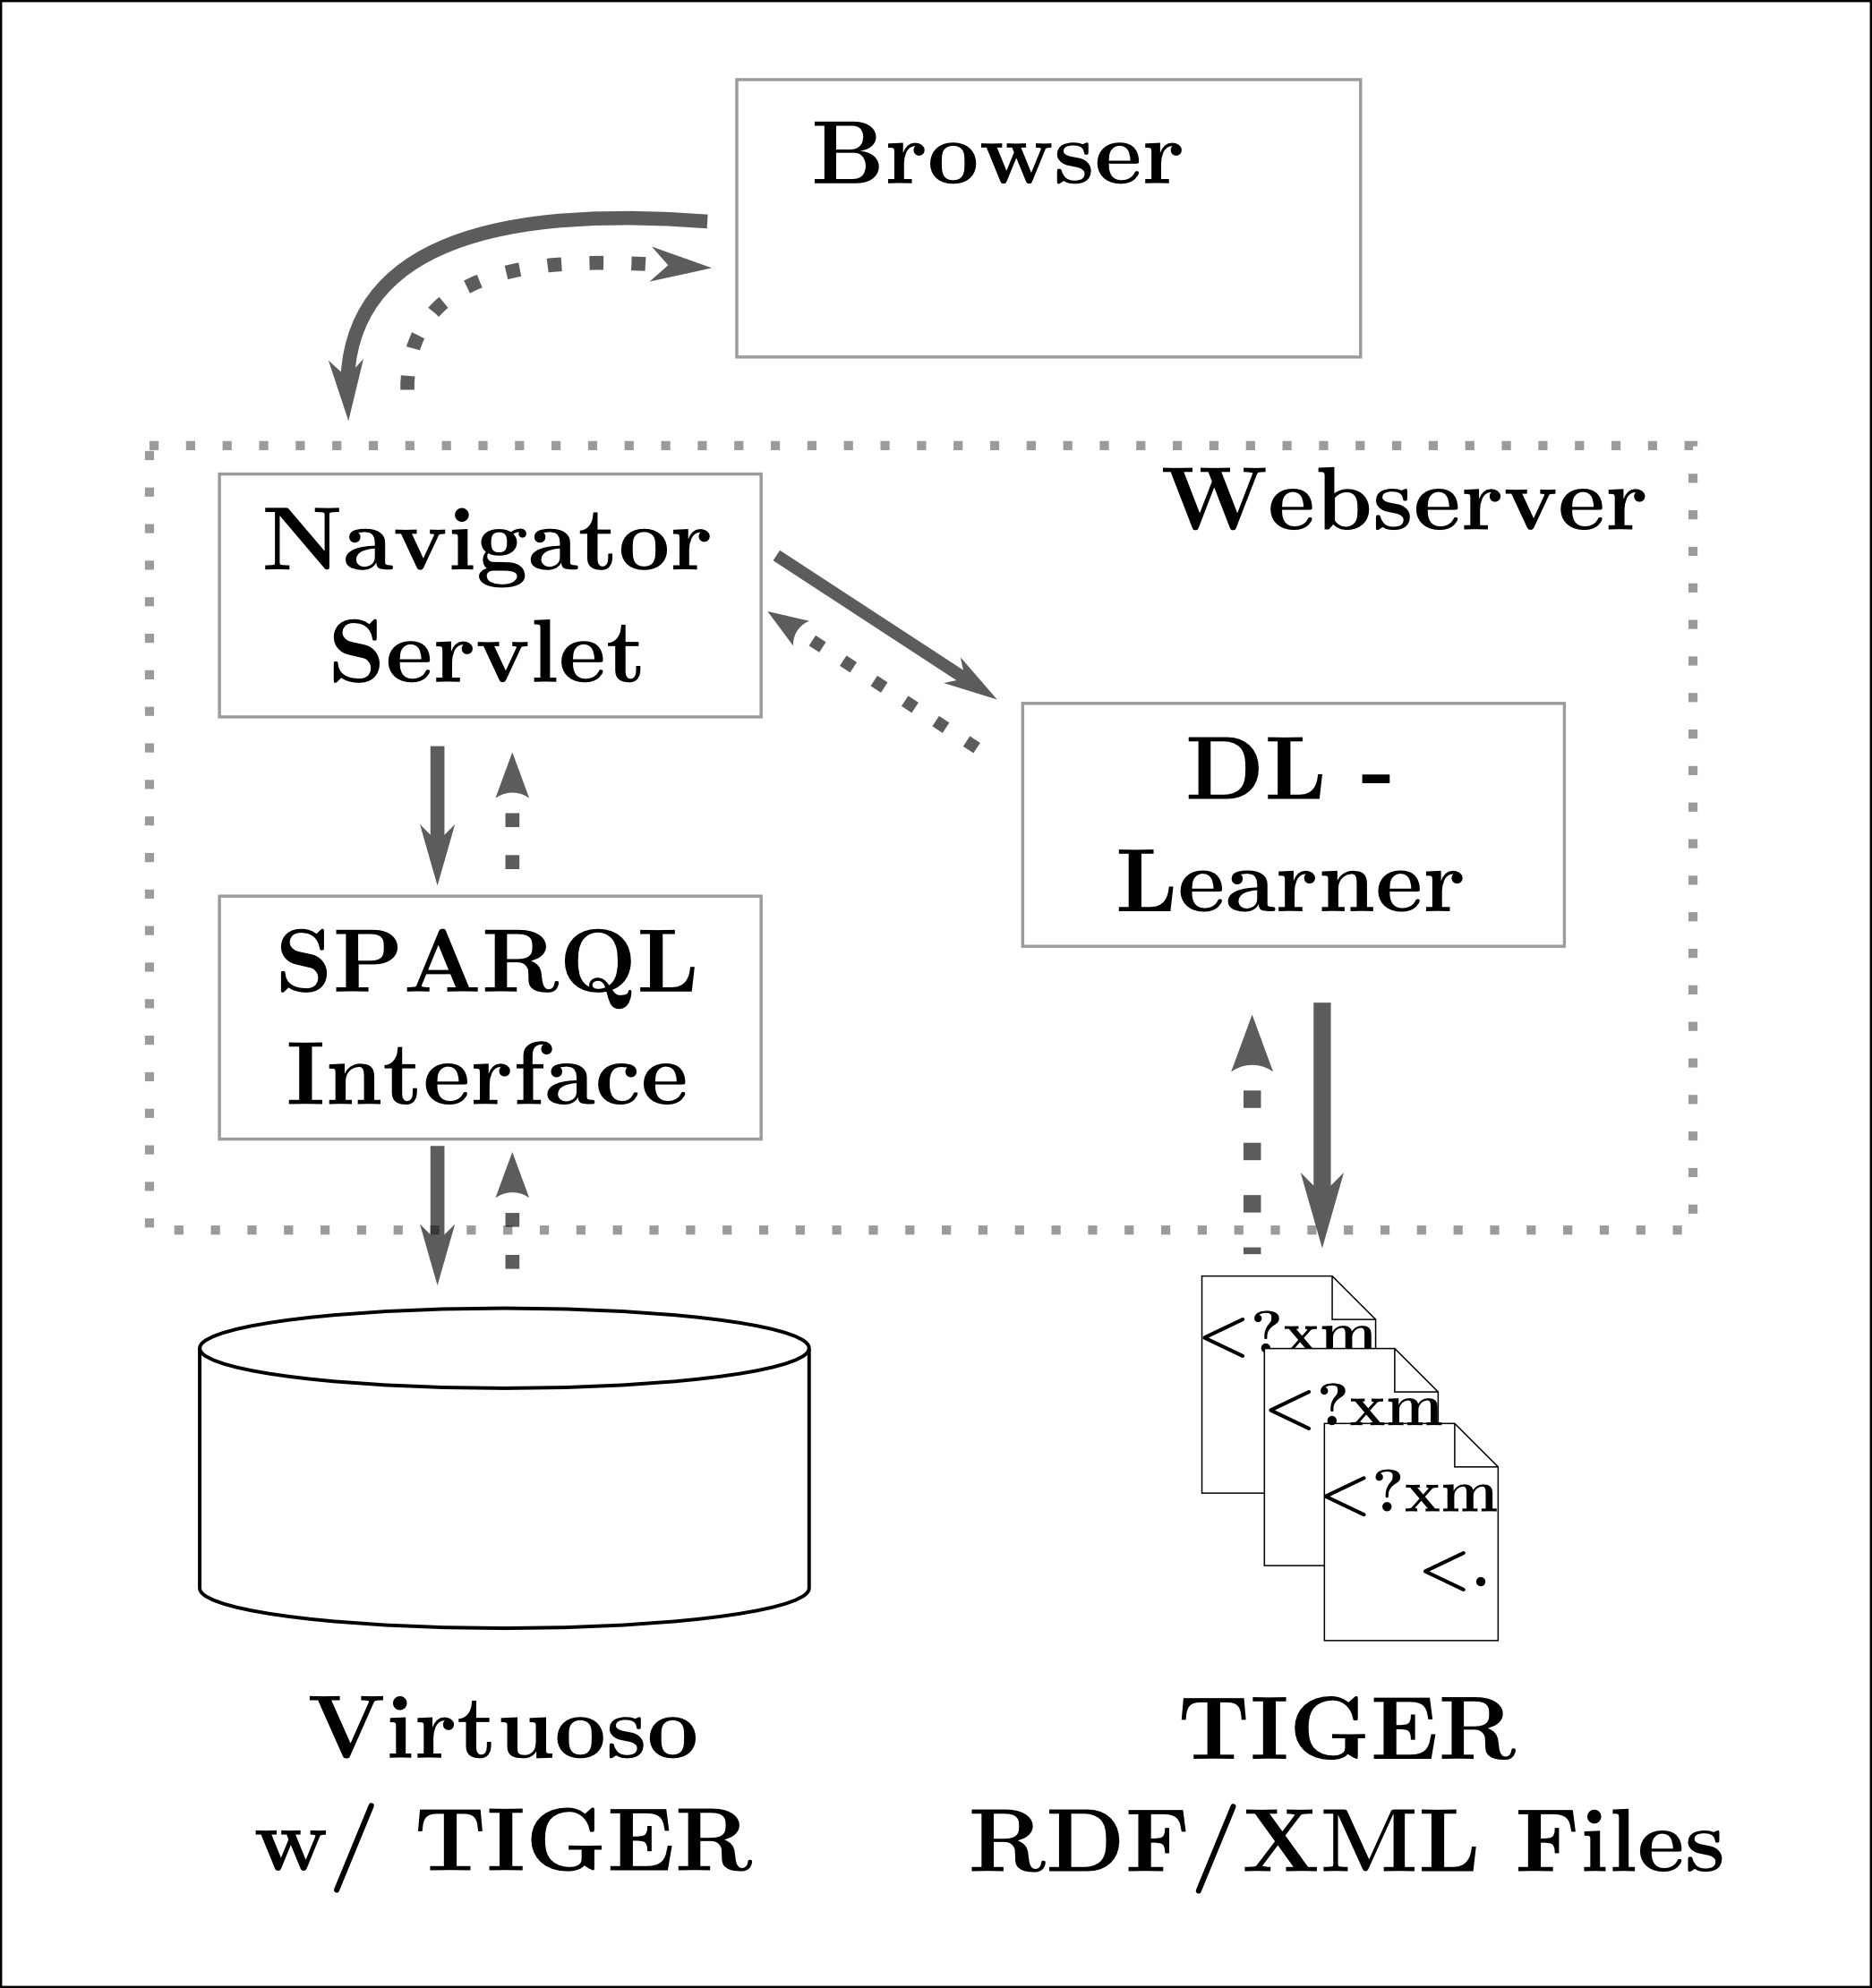
\includegraphics[width=0.5\textwidth]{img/tigercorpusnavigator_architecture.png}
\begin{tablenotes}\footnotesize
 \item [] Quelle: \citet{tiger_corpus_navigator}
\end{tablenotes}
\end{threeparttable}
\caption{Die technische Architektur des TIGER Corpus Navigators}
\label{fig:tigercorpusnavigator_architecture}
\end{center}
\end{figure}

Durch die Verwendung von NLP2RDF ergibt sich jedoch ein wesentlich einfacherer Ansatz (siehe Abbildung \ref{fig:tigercorpusnavigator_architecture}):
Aus allen Sätzen des Korpus werden mitsamt ihrer Annotationen RDF-Strukturen erzeugt, die in einem \emph{Virtuoso Triple Store} gespeichert sind.
Die den ausgewählten Sätzen zugehörigen RDF-Strukturen dienen als Eingabe für den \emph{DL-Learner}\footnotemark, ein Programm, welches Konzepte in Beschreibungslogiken, wie OWL, anhand von Beispielen lernt.
\footnotetext{beschrieben in \citet{dl-learner}, Projektseite \url{http://dl-learner.org/Projects/DLLearner}}

%Mithilfe dieses Ansatzes kann der TIGER Corpus Navigator erfolgreich mehrere Datenquellen 

%es konnte bereits erfolgreich die definition für einen passivsatz gelernt werden
%-> hier die owl regel dafür hinschreiben
%tigercorpusnavigator_screenshot.png
\chapter{Wortschatz2DBpedia}\label{sec:wortschatz2dbpedia}

\begin{dfn}
\emph{"`Ein \emph{Mapping}\footnote{engl. mapping [comp.] = Abbildung,Zuordnung} ist eine Menge paarweiser Zuordnungen, sogenannter Korrespondenzen, zwischen Instanzdaten.
Dabei wird in dieser Arbeit mit dem Begriff Korrespondenz nicht nur die Verknüpfung gleicher Objekte gemeint, sondern allgemein eine Beziehung zwischen zwei Objekten ausgedrückt."'}\citep{thor-dissertation}

%Diese Definition ist der Dissertation von Dr. Andreas Thor entnommen .
Ein Mapping erlaubt damit komplexe Anfragen, die mit den Datenquellen allein nicht möglich wären.
Es erlaubt auch die Aggregation von Informationen verschiedener Art über ein Objekt.\footnote{in dieser Arbeit sowohl statistische als auch semantische Informationen über Wörter}
\end{dfn}

\section{Anforderungen}\label{sec:anforderungen}
%1239916 wortschatz2dbpedia/input/wortschatz/en_words_all.txt

Aufgabe ist es, ein Programm zu implementieren, welches ein Mapping zwischen dem \emph{Projekt Deutscher Wortschatz} (sowie seiner internationalen Version) und der \emph{DBpedia} generiert.
Eine solche Verknüpfung verbindet jeweils eine Ressource des Wortschatzes mit einer Ressource der DBpedia.
Eine Ressource beim Wortschatz ist eine Wortform. Eine DBpedia-Ressource ist eine RDF-Entität, welche automatisch extrahierte strukturierte Informationen aus einem Wikipediaartikel enthält und 
dabei ein Objekt oder Konzept aus der realen Welt beschreibt.
Das Programm muss einmal pro Jahr von einer Fachkraft ausgeführt werden, um mit den jährlich aktualisierten Wortschatzdaten ein neues Mapping herzustellen.
Die Anforderungsanalyse ergab dabei Folgendes:

\subsection{Funktionale Anforderungen}
Aufgabe des Programmes ist die Erstellung eines Mappings zwischen DBpedia und dem Internationalen Wortschatzprojekt in einer bestimmten Sprache.
Das Mapping besteht aus Links zwischen Wörtern des Wortschatzprojektes und Ressourcen der DBpedia.
Dabei sind zunächst einmal nur die englischen und deutschen Versionen zu verarbeiten, eine einfache Erweiterung auf andere Sprachen soll jedoch garantiert sein.
Die Wörter entstammen dem Corpus des Wortschatzprojektes und enthalten daher sowohl Einzelne- ("`\emph{Brot}"'), als auch Mehrwörter ("`\emph{SPD Generalvorsitzender Frank Walter Steinmeyer}"'),
 wie sie im normalen schriftlichen Gebrauch ausgewählter Quellen (Zeitungen und zufällig ausgewählte Webseiten) enthalten sind.
Die DBpedia-Ressource eines bestimmten Namens ist eine RDF-Entität, welche automatisch extrahierte, strukturierte maschinenverarbeitbare Informationen 
aus dem gleichnamigen Wikipediaartikel enthält und damit ein Objekt oder allgemeiner ein Konzept der realen Welt repräsentiert.
\begin{center}
\begin{tabular}{ll}
\toprule
DBpedia-Ressource & \url{dbpedia:London_Heathrow_Airport}\\
rdfs:label & London Heathrow Airport\\
Wikipedia Titel & London Heathrow Airport\\
Wikipedia URL & \url{en-wiki:London_Heathrow_Airport}\\
\bottomrule
\end{tabular}
\end{center}

\begin{dfn}\label{dfn:korrekte_korrespondenz}
Ein Paar $(w,a)$, wobei $w$ eine Wortform des englischen Wortschatzes und $a$ ein Artikelname der englischen Wikipedia ist, ist eine \emph{Korrespondenz}.
Es existiert dann sowohl ein Wikipediaartikel \article{en-wiki:}$a$ als auch eine DBpedia-Entität \article{dbpedia:}$a$.
Eine Korrespondenz gilt genau dann als \emph{korrekt}, wenn das Konzept, das von der Entität beschrieben wird, mit der Wortform benannt werden kann.
Das Konzept ist dann eine der möglichen Bedeutungen des Wortes.
\end{dfn}

Ist der Titel eines Wikipediaartikels mit einer Wortform identisch, dann bilden der Artikelname und die Wortform einen korrekten Link, da ein Titel eine Form der Benennung ist.
Da ein Titel aber immer groß geschrieben wird, sind hier zwei Arten von Fehlern möglich:
\begin{enumerate}
 \item Die Wortform ist identisch mit dem Artikelname, dieser wird jedoch normalerweise klein geschrieben, das Paar ist also inkorrekt.
 \item Die Wortform wird klein geschrieben, ist aber ansonsten identisch mit dem normalerweise klein geschriebenen Artikelnamen, das korrekte Paar wird also nicht erkannt.
\end{enumerate}
Da es jedoch keine Möglichkeit gibt, die wirkliche Großschreibung des ersten Buchstabens des Titels herauszufinden, wird die Großschreibung des ersten Buchstabens ignoriert und auch Paare mit 
verschiedener Großschreibung des ersten Buchstabens werden als identisch betrachtet.
Trotzdem wird in der Analyse in Abschnitt \ref{sec:analyse} die Präzision groß- und kleingeschriebener Wortformen getrennt aufgeschlüsselt, wobei das Existieren des Artikelnamens als Benennung ignoriert wird
(sonst hätten ja alle diese Paare nach Definition \ref{dfn:korrekte_korrespondenz} eine Präzision von \valunit{100}{\%}).

Ein solches minimales Mapping, das genau die identischen Paare umfasst ist leicht erzeugbar, %(\valunit{100}{\%} nach Definition \ref{dfn:korrekte_korrespondenz}),
enhält aber nur wenige Korrespondenzen (\val{13798} mit den Eingabedaten, die in Abschnitt \ref{sec:analyse} verwendet werden, also \valunit{11.6437}{\%} des dort erzeugten groben Mappings).
Durch verschiedene Methoden können auch nicht identische Paare mit gleicher Bedeutung gefunden werden.
Eine Möglichkeit dies zu tun ist, eine Ähnlichkeitsfunktion \s{} einzuführen, welche für eine Korrespondenz $(w,a)$ eine reelle Zahl zwischen $0$ (komplett verschieden) und $1$ (exakt gleich) annimmt.
Für jedes Wort $w$ und jeden Artikelnamen $a$ solch eine Ähnlichkeitsfunktion $\s(w,a)$ auszuwerten, würde jedoch zu einer aufgrund der großen Datenmenge nicht akzeptablen quadratischen Laufzeit führen,
denn bei einer groben Schätzung mit drei Millionen Wörtern\footnote{In der Analyse wurde nur das englische Normkorpus mit einer Million Sätzen verwendet, das gesamte Korpus ist jedoch wesentlich größer.}
und DBpedia-Ressourcen sowie angenommenen einer Million Vergleichen pro Sekunde ergibt sich eine Laufzeit von $3\frac{1}{2}$
Monaten.\footnote{$\frac{(3\cdot 10^6)^2\textnormal{Vergleiche}}{10^6 \textnormal{Vergleiche/s}} = 9 \cdot 10^6 \textnormal{s}$}


%\subsubsection{Stringtransformatoren}
Aus Laufzeitgründen soll das erweiterte Matching über die Entfernung von für die Wortdifferenzierung unwichtigen Merkmalen erfolgen.
Dies geschieht, in dem vor dem Matching eine Funktion $t: \textnormal{String} \rightarrow \pow{\textnormal{String}}$ (hier als \emph{Stringtransformator} bezeichnet) auf $w$ und $a$ ausgeführt wird.
Nun werden dem Matching alle Paare $(x,y), x \in \func{t}(w), y \in \func{t}(a)$, hinzugefügt. Dieser Vorgang wird auch als \emph{Termnormalisierung} bezeichnet.
Da die meisten in dieser Arbeit benutzten Stringtransformatoren immer einelementige Ergebnismengen erzeugen, werden diese aus Übersichtsgründen im Folgenden auch 
als Funktionen vom Typ $\textnormal{String} \rightarrow \textnormal{String}$ und einelementige Mengen als einzelne Zeichenketten dargestellt .
%Welche dieser Stringtransformatoren das beste Ergebnis bringen, wird mithilfe einer manuellen Analyse in Abschnitt \ref{sec:analyse} bestimmt.

\begin{bsp}
Sei $\func{t}=\func{String.toLowerCase()}$. Beim Matching wird nun die Groß- und Kleinschreibung ignoriert und das Paar (Cattle,cattle) gefunden.
\end{bsp}

Es sind auch Transformatoren möglich, die bestimmte Wortmengen ausschließen, deren Präzision sich als niedrig herausstellt,
indem sie diese Wörter auf das leere Wort $\epsilon$ abbilden, welches von der weiteren Verarbeitung ausgenommen ist.
Diese Transformatorfunktionen sollen auch vom Benutzer frei ausgewählt werden, auch die Hintereinanderausführung $\func{t}_1(\func{t}_2(...\func{t}_n(w)...)$ sowie das Vereinigen von Matches mit verschieden Transformatoren soll möglich sein. 
Welche dieser Methoden letztendlich verwendet werden, ergibt sich aus deren Analyse in Abschnitt \ref{sec:analyse}.

\iffalse
Eine Anwendung wäre das Einblenden der zu einem Wort zugeordneten Ressourcen mit Hilfe eines Links auf der Wortschatzseite zu diesem Wort, sodass sich ein Nutzer des Wortschatzes über die Bedeutung eines Wortes informieren kann.
Laut Herrn Volker Böhlke\footnotetext{http://www.informatik.uni-leipzig.de/personal/VBoehlke.html}, einem Mitarbeiter des Wortschatzprojektes, sind es die Nutzer einschlägiger Suchmaschinen gewöhnt, dass sie mehrere Möglichkeiten haben  um dann selbst den für sie geeignetsten Treffer auszuwählen.
In diesem Fall ist es daher besser, einen Anteil unpassender Verweise dabei zu haben, als das Risiko einzugehen, dass das Gesuchte nicht dabei ist.
Beim Einsatz in einer Kette von Verarbeitungsschritten, wie in Abschnitt \ref{sec:disambiguierung} beschrieben im Rahmen einer Wortsinndisambiguierung, können falsche Matches jedoch unerwünschte Fehlausgaben des Programmes liefern.
Aus diesen Gründen soll es zwei Typen von Links geben: diejenigen, bei denen eine hohe - (der sichere Link) und jene, bei denen eine etwas niedrigere Präzision erwartet wird (der alternative Link).
Als Grundlage kann von einem sicheren Link $(r,w)$ ausgegangen werden, wenn das Wort $w$ mit dem Namen $r$ der DBpedia-Ressource übereinstimmt, $r=w$. Dies sollte sich in linearer - und damit akzeptabler - 
Laufzeit implementieren lassen\footnote{Pseudocode: \code{für alle e aus Menge1: if(Menge2 enthält e) Mapping.add(e,e)}. Wenn Menge2 in einer Hash-basierten Datenstruktur gehalten wird, ist ein Zugriff in konstanter Zeit möglich.}.
Der Namen der Ressource ist ja auch der Name eines Artikels über das beschriebene Konzept, und damit ist $r$ und damit auch $w$ eine Benennung des Konzeptes.
Um die Coverage zu erhöhen, ist nun der nächste Schritt das Verknüpfen von Wörtern mit DBpedia-Ressourcen, deren Name nur noch ähnlich aber nichtmehr exakt gleich ist.
\fi

\subsubsection{Korrektheit}
Das Programm soll die ausgewählten Matchingroutinen natürlich fehlerfrei ausführen.
Aufgrund der großen Menge an Eingabedaten in der Größenordnung von mehreren Millionen und der Komplexität des Problems ist jedoch eine gewisse Menge an Fehlverknüpfungen unvermeidlich.
%Außerdem ist es schon eine Herausforderung an sich, eine exakte Definition zu finden, wann eine Verknüpfung korrekt ist [siehe insert verweis here], und diese anhand einer großen Zahl von Verknüpfungen zur  Überprüfung anzuwenden.
Bestimmte Verfahren besitzen zwar eine gewisse Fehlerquote, können jedoch den Anteil der gefundenen Verknüpfungen, die Coverage, wesentlich erhöhen.
Andere Methoden können zwar einige wenige weitere Verknüpfungen finden oder Fehlerhafte vermeiden, würden jedoch die Performance oder Entwicklungszeit unverhältnismäßig erhöhen.
Es muss also ein Kompromiss zwischen Laufzeit, Präzision, Coverage und Entwicklungszeit gefunden werden.
Links mit erwarteter hoher bzw. niedrigerer Präzision sind jedoch durch verschiedene Linktypen zu kennzeichnen.
%Auch wenn wir kaum Anforderungen an Geschwindigkeit stellen, würde aufgrund der großen Datenmenge ein Algorithmus quadratischer Laufzeitkomplexität (wie er vorliegt, wenn wir jedes Element der Einen mit jedem Element 
%der anderen Menge vergleichen) eine nicht tolerierbare Ausführungszeit haben.

\subsubsection{Redirects}
Das Matching soll auch Wikipedia - Redirects mit einbeziehen.
Redirects sind keine richtigen Artikel sondern nur Weiterleitungen.
Wenn man beim englischen Wikipedia \zb{} "`cow"' eingibt, wird man auf den Artikel "`cattle"' weitergeleitet.
Dies wird auch bei der Extraktion des Artikels zur DBpedia-Ressource vermerkt.
Diese Redirects sollen dabei für den Matchingvorgang wie normale Ressourcen betrachtet werden, danach aber auf das Ziel des Redirects geändert werden.

\begin{bsp}
Die Wortform "`cow"' wird untersucht, eine passende Ressource wird nicht gefunden, jedoch existiert der redirect \emph{cow}$\rightarrow$\emph{cattle},
\emph{cow} wird also erst auf \emph{cow} gemappt, hinterher jedoch werden die Redirects aufgelöst und das Paar wird zu $(\emph{cow},\emph{cattle})$ geändert.
\end{bsp}

\subsubsection{Mehrwortbegriffe}
Mehrwortbegriffe werden auch mit einbezogen, ein mögliches Mapping wäre (Franz Müntefering,Franz Müntefering).
Das Matching von Mehrwortbegriffen, die in anderen enthalten sind, soll nicht vorgenommen werden.
Mappings wie ((der) SPD Vorsitzende Franz Müntefering,Franz Müntefering) sind zwar richtig, müssen aber aufgrund des nicht angemessenen technischen Aufwandes nicht berücksichtigt werden.
Nehmen wir an, wir vergleichen den Mehrwortbegriff "`Gartenvorstand Peter Müller"' und eine Ressource namens "`Peter Müller"'.
Ob dieses Paar in unserem Sinne korrekt ist hängt nun davon ab, ob der Artikel tatsächlich einen Peter Müller beschreibt, der auch Gartenvorstand ist.
Dies lässt sich alleine aus dem Artikelnamen ohne Zusatzwissen jedoch nicht herausfinden.
Eine Möglichkeit wäre zwar, den Artikel nach dem Mehrwort "`Gartenvorstand Peter Müller"' zu durchsuchen, aber dann würde man immer noch Sätze wie 
"`es handelt sich in diesem Artikel nicht um den Gartenvorstand Peter Müller"' erkennen.
Das Vorkommen derartiger Matches wird dem Aufwand nicht entsprechend geschätzt, trotzdem soll die Möglichkeit, das Programm später auf Derartiges zu erweitern gegeben sein.

\subsection{Nichtfunktionale Anforderungen}

\subsubsection{Zuverlässigkeit}
Es werden keine Anforderungen an die Fehlertoleranz gegenüber Benutzereingabefehlern gestellt.
Eine Fehlermeldung ("`Ihre Eingabedatei besitzt ein ungültiges Format"') genügt.
Einzelne Fehleinträge in den Eingabedaten sollen jedoch nicht zum Abbruch des Programmes führen, sondern einfach ignoriert werden.

\subsubsection{Aussehen und Handhabung}
Es werden keine Anforderungen an das Aussehen und die Handhabung gestellt.
Eine Bedienung per Kommandozeile mit einer Ausgabe der zu erwarteten Parameter bei Fehleingabe genügt.

\subsubsection{Benutzbarkeit}
Es werden keine Anforderungen an das Aussehen und die Handhabung gestellt.

\subsubsection{Leistung und Effizienz}
Es werden keine signifikanten Anforderungen an die Laufzeit des Programmes gestellt, Laufzeiten von bis zu mehreren Tagen sind also explizit erlaubt. In solch einem Fall muss aber eine Vorschau implementiert werden.

\subsubsection{Betrieb und Umgebungsbedingungen}
Das Programm ist in Java zu implementieren und sollte daher überall laufen, wo eine standardkonforme Java Virtual Machine vorhanden ist.
Betrieben wird das Programm jedoch am Ende wohl auf einer Windows- oder Linuxplattform, sodass nur diese beiden zu garantieren und zu testen sind.

\subsubsection{Wartbarkeit, Änderbarkeit}
%Laut Herrn Boehlke wird im Wortschatzprojekt immer noch ein Programm eingesetzt, welches im Rahmen einer Diplomarbeit von vor über 10 Jahren entstand
%Dieses wird heute noch genutzt, aufgrund fehlender Analysierbarkeit und Erweiterbarkeit ist es jedoch mittlerweile Anfang einer Kette von Scripts, welche dessen Ausgabe im ursprünglich erforderlichen Format aufbereiten und in das mittlerweile Erforderliche bringen.
%Auch wenn der Autor nicht weiss, ob sein Programm ähnlich lange in Gebrauch sein wird, hofft er doch, dass ihm ein ähnliches Schicksal erspart bleibt.
Das Wortschatzprojekt besteht bereits seit über 10 Jahren und wird aufgrund seiner Popularität wohl noch lange in Gebrauch sein.
Die DBpedia nimmt eine zentrale Rolle für Linked Data ein.
Aus diesem Grunde soll das Programm auf erwartete Änderungen vorbereitet sein.
Eine ordentliche Umsetzung objektorientierter Prinzipien und Design Patterns wird also vorausgesetzt.
Insbesondere die Datenquellen und Vergleichsalgorithmen sollen ohne weitere Kenntnisse der Programmstruktur trivial erweiterbar sein.
Bestehende Programmroutinen müssen jedoch nur ein Grundmaß an Kommentaren aufweisen, welches erwartete Eingabe, Funktion und Ausgabe jedes Moduls beschreibt.
Es werden keine signifikanten Anforderungen an die Analysierbarkeit des Programmes gestellt.

\subsubsection{Portierbarkeit und Übertragbarkeit}
Es werden keine Anforderungen an die Portierbarkeit gestellt, aufgrund der Implementierung in Java ist diese jedoch ohne weiteren Aufwand gegeben.
Es reicht eine einfache Readme-Datei, welche den Installationsvorgang erklärt.
Die Sprache sowohl des Quelltextes, der Benutzerschnittstelle als auch der Dokumentation kann zwischen deutsch und englisch frei gewählt werden.

\subsubsection{Sicherheitsanforderungen}
Da Teile des Wortschatzes nicht frei verfügbar sind, dürfen diese Teile nicht in frei zugänglichen Distributionen des Programmes enthalten sein.
Weiterhin dürfen die geschützten Daten auch nicht aus dem Programm generierbar sein, falls es auf diese keinen Zugriff hat.
%Dieser Fall ist daher möglich, da bestimmte Informationen im Einzelzugriff frei verfügbar, in einer Komplettfassung jedoch kostenpflichtig sind.

\subsubsection{Flexibilität}
Das Programm soll die Daten so akzeptieren, wie sie auf der Webseite der DBpedia\footnote{\url{http://wiki.dbpedia.org/Downloads}} und des Wortschatzes\footnote{\url{http://corpora.informatik.uni-leipzig.de/download.html}} herunterladbar sind.
Falls sich deren Format ändert, soll es auf einfache Art und Weise so erweiterbar sein, dass es dieses verarbeiten kann.
Die Programmparameter sind aus einer Datei im INI-Format auszulesen.

\subsubsection{Skalierbarkeit}
Das Programm soll in der Lage sein, mit Datenmengen von mehreren Millionen Wörtern und DBpedia-Ressourcen umzugehen.

%\subsubsection{Entwicklungsdauer}
%Die Entwicklungsdauer sollte einen Monat nicht wesentlich überschreiten.
\section{Analyse}\label{sec:analyse}
Im Folgenden wird ein Mapping des Prototypen mit \val{118425} Einträgen analysiert, bei dessen Erstellung die \val{260880} Wörter des englischen Normcorpus mit einer Million Sätzen und \val{3201391} Artikelnamen miteinander verglichen wurden.

\subsection{Das Matching}
Der Matching läuft immer auf die gleiche Art und Weise ab:
Es werden die Datenquellen für den Wortschatz $D_w$ und die DBpedia $D_d$ festgelegt und ein Stringtransformator t ausgewählt.
Danach wird der Stringtransformator auf die Wortlisten der beiden Datenquellen angewendet und alle Paare $(a,w)$, $a\in D_d$, $w\in D_w$ mit $\func{t}(a)=\func{t}(w)$ werden dem Mapping hinzugefügt.
Üblicherweise ist dieser Stringtransformator eine Instanz der Klasse StringTransformatorList, das heißt eine Hintereinanderausführung mehrerer Stringtransformatoren.
Für die Stichprobenanalyse wird ein sehr grobes Mapping verwendet, das möglichst viele Paare abdeckt. Eine Auswertung der Präzision dieses Mappings und seiner Teile bestimmt, welche Stringtransformatoren für das
Erstellen des finalen Mappings letztendlich verwendet werden.
%Da eine Stichprobenanalyse sehr zeitaufwändig ist, wurde ein sehr grobes Mapping erzeugt, welches möglichst alle folgenden Mappings enthalten sollte, auch wenn dies zu Lasten der Präzision geht.
\paragraph{}
Die Eingabedaten sind:
\begin{itemize}
\item die zu diesem Zeitpunkt\footnote{Datum des Dumps: 20.5.2009} komplette Artikelliste der englischen DBpedia\footnote{\url{http://downloads.dbpedia.org/3.3/en/articles_label_en.csv.bz2}}
\item die Wörter aus einem Teilcorpus\footnote{\url{http://corpora.uni-leipzig.de/resources/flatfiles/en1M.zip}} des englischen Wortschatzes (eine Million Sätze zufällig ausgewählt aus dem Hauptcorpus)
\end{itemize}

Einträge unter drei Buchstaben werden nicht in das Mapping einbezogen,
Sonderzeichen und Unterschiede in der Groß- und Kleinschreibung werden komplett ignoriert, sowie sämtliche Vorkommen von "`(disambiguation)"', um auch Disambiguierungsseiten mit einzubeziehen.

\begin{lstlisting}
StringTransformer transformer = 
 new StringTransformerList
 (
  new RemoveSpecialCharactersTransformer(),
  new MinimumLengthTransformer(3),
  new LowerCaseStringTransformer(),
  new RemoveDisambiguationTransformer()
 );
\end{lstlisting}
\subsection{Die Stichprobe}
Die Stichprobe besteht aus 200 zufällig ausgewählten Zeilen des Mappings\footnotemark{}.
\footnotetext{Das Erstellen einer Stichprobe erfolgt mittels "`\texttt{rlines <dateiname> <zeilenanzahl>}"'. \emph{rlines} ("`random lines"') gehört zum Projekt wortschatz2dbpedia und ist von dessen svn-Server herunterladbar.}% Die Syntax ist "`\texttt{rlines dateiname zeilenanzahl}"'.}
%\footnotetext{\url{http://wortschatz2dbpedia.googlecode.com/svn/trunk/}}
%\begin{verbatim}
Jeder Eintrag der Stichprobe ist von Hand als entweder korrekt oder inkorrekt bewertet,
wobei ein Eintrag \emph{(Artikelname, Wortform)} genau dann als korrekt zählt, wenn eine der Bedeutungen der Wortform im Wortschatz mit der Bedeutung übereinstimmt,
die im zugeordneten Wikipediaartikel und der DBpedia-Entität beschrieben ist.
Die Bedeutungen einer Wortform im Wortschatz wird dabei durch dessen Kookurrenzen, linke und rechte Nachbarn und Beispiele erfasst.
\texttt{
\begin{table}
 \begin{tabular}[b]{ll}
\toprule
\textnormal{DBpedia}&	\textnormal{Wortschatz}\\
\midrule
PCL		&PCL\\
Baird		&Baird\\
Théodore	&Theodore\\
Impossible	&`Impossible\\
Cat		&`cat\\
Perversity	&perversity\\
Braniff		&Braniff\\
Museum		&museum\\
Times-Journal	&Times-Journal\\
Oviedo		&Oviedo\\
Refugium	&refugium\\
Wachtel		&Wachtel\\
Mandolin	&mandolin\\
D.b.s.		&DBs\\
Oyo		&Oyo\\
Abundant	&Abundant\\
Elkhorn		&elkhorn\\
Waryś		&WARY\\
Moorings	&moorings\\
Tan-tan		&Tan-Tan\\
Subcontractor	&sub-contractor\\
K.I.N.G.	&king\\
AirPort		&Airport\\
Reserve		&REserve\\
PLE		&P\&LE\\
\ldots\\
\bottomrule
\end{tabular}
\caption{Ein Ausschnitt der Stichprobe}
\end{table}
}\\

Jeder Eintrag der Stichprobe ist als entweder augenscheinlich korrekt oder inkorrekt festgelegt,
wobei als Hinweise auf die Bedeutung einer Wortform die im Wortschatz angegebenen Kookurrenzen, linken und rechten Nachbarn und Beispiele gelten.
Stimmt diese Bedeutung mit der im zugeordneten Wikipediartikel und in der DBpedia-Entität beschreiben Bedeutung überein, dann gilt der Eintrag als korrekt, ansonsten als inkorrekt.


\begin{bsp}
Wir möchten das Paar \emph{(Subcontractor,sub-contractor)} validieren.
Betrachten wir die Ressource \url{dbpedia:Subcontractor}, so finden wir unter anderem die Einträge
\begin{quote}
\url{skos:subject}
\begin{itemize}
\item \url{dbpedia:Category:Construction}
\item \url{dbpedia:Category:Contract_law}
\end{itemize}
\end{quote}

Ein \emph{Subcontractor} hat also etwas mit Konstruktion und mit Vertragsgesetzen zu tun.
Im Wortschatz finden wir dazu ein passendes Beispiel:
%\hline
%\fbox{ \begin{minipage}{\linewidth}
\begin{webseitenausschnitt}
\textbf{term}: sub-contractor\\
\ldots\\
\textbf{example(s):}\\
We had left the civilised world of museums for the harsh realities of the \ovalbox{construction industry}, where we faced all the problems of the sub-contractor. (source: \emph{Financial Times 1994})
%\end{minipage}}
\end{webseitenausschnitt}
Das Paar ist also korrekt.
\end{bsp}
\iffalse
\begin{rem}
Die Korrektheitsdefinition eines Paares $(d,w)$ war zu diesem Zeitpunkt noch 
"`Der DBpediaartikel $d$ (oder die zugehörige Wikipediaseite) beschreibt ein Konzept, welches im Wortschatzcorpus mindestens in einem Fall durch das Wort $w$ benannt wird"'.
Nach dieser Definition können also euch exakte Matches $d=w$ inkorrekt sein.
Nach einem Gespräch mit Herr Volker Boehlke wurde jedoch eine schwächere Definition benutzt, nämlich, dass das Konzept nur noch in irgendeinem Kontext durch das Wort $w$ benannt wird,
 ohne dass dieser Fall im Corpus des Wortschatzes auftreten muss.
Daraus folgt unter anderem, dass exakte Matches nun per Definition als korrekt gelten, denn der Name des Wikipediaartikels ist ja schon eine Benennung des Konzeptes.
Trotz dieser leichten Veränderung der Definition bleibt die Analyse der Stichprobe relevant.
Da die Validierung der Stichprobe anhand des Wortschatzeintrages erfolgt, werden sowieso nur die Fälle überprüft, die im Wortschatz vorkommen.
Einzige Ausnahme sind die exakten Matches, die wir aber auch so immer in unser Mapping einschließen.
Die hier bestimmten Genauigkeitswerte sind also untere Schranken für den Wert, der anhand der aktuellen Definition bestimmt werden würde. Die Abweichungen dürften aber minimal ausfallen.
\end{rem}
\fi

\subsection{Betrachtung der gesamten Stichprobe}
Von den 200 Einträgen der Stichprobe sind 85 als korrekt bestimmt. Die geschätzte Genauigkeit (Precision) des Mappings liegt also bei $\valunit{42.5}{\%}$.
Das $\valunit{95}{\%}$-Konfidenzintervall
liegt bei $[71,99]$, also $[\valunit{35.5}{\%},\valunit{49.5}{\%}]$.
Die in den folgenden Diagrammen angegebenen Prozentwerte sind ganzzahlig abgerundet. Bei Angabe der Konfidenzintervalle\footnotemark{} ist die linke Grenze ab- und die rechte Grenze aufgerundet auf zwei Nachkommastellen.
\footnotetext{errechnet mit \url{http://www.matheprisma.de/Module/Hypoth/konfi2.htm}, Binomialverteilung}
\subparagraph*{Zusammensetzung}~\\
%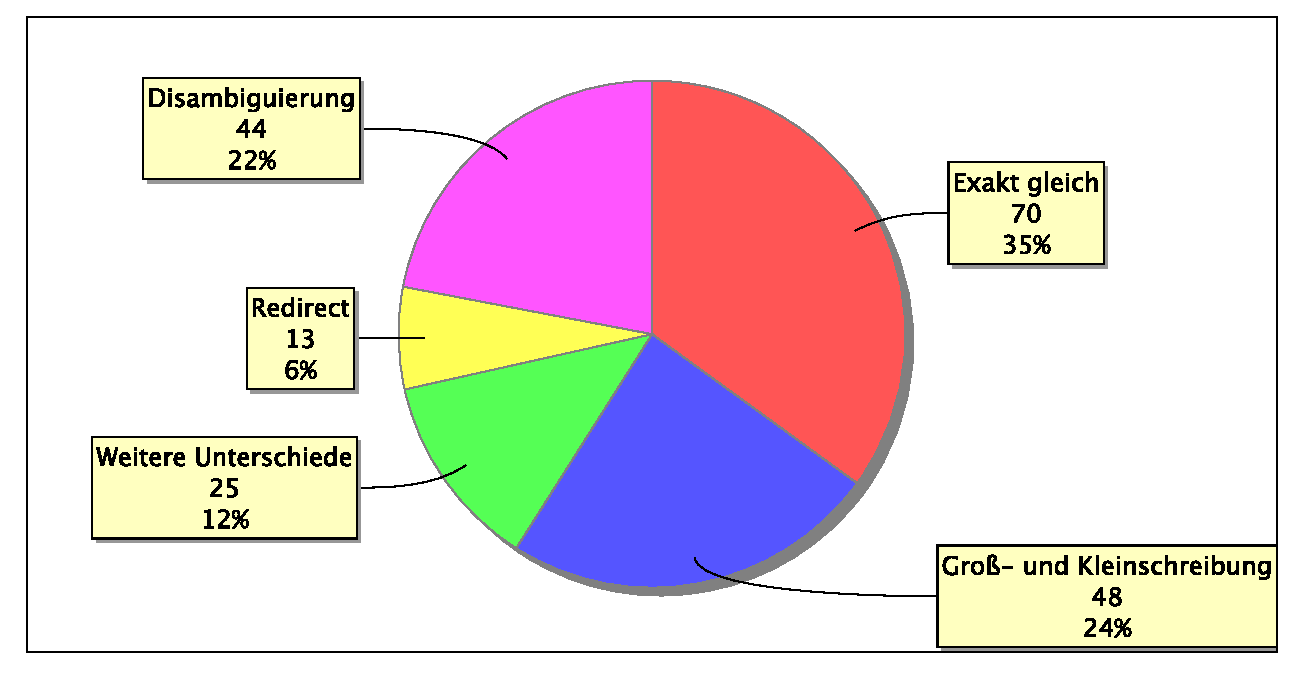
\includegraphics[width=\textwidth]{wortschatz2dbpedia/analyse/mapping1/stichprobe1/wortschatz2dbpedia.analyse.GeneralClassifier.piechart.eps}
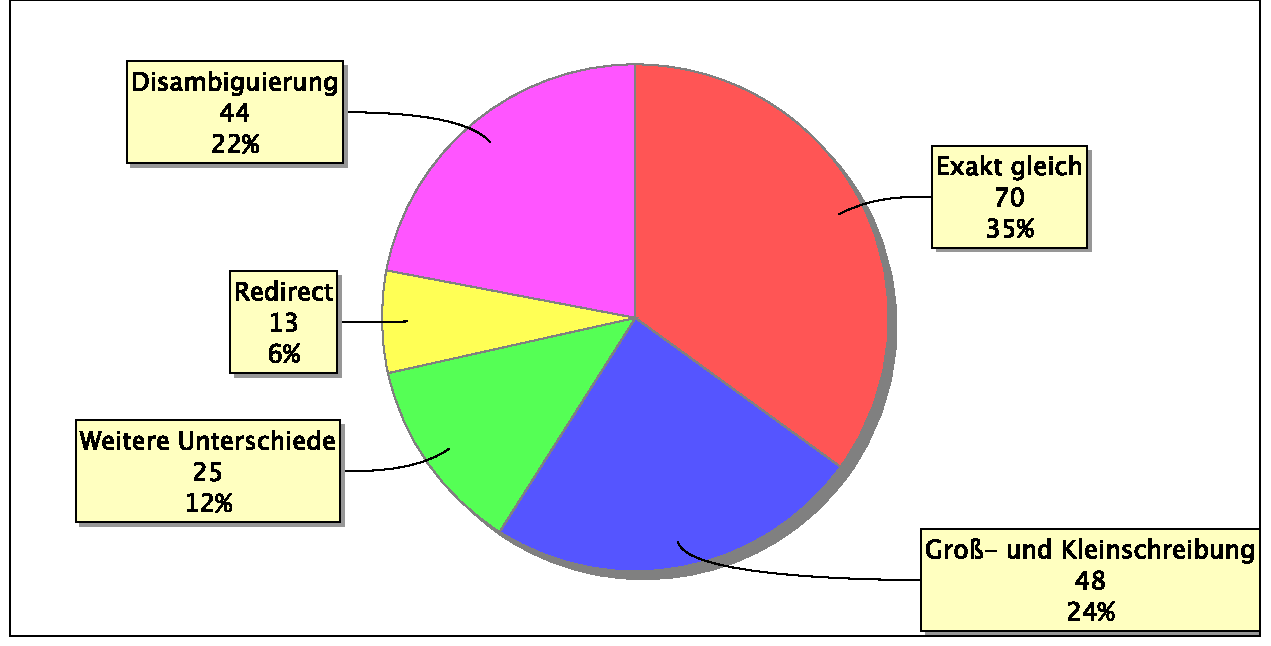
\includegraphics[width=\textwidth]{img/pdf/wortschatz2dbpedia.analyse.GeneralClassifier.piechart.pdf}
\subparagraph*{Genauigkeit}~\\
%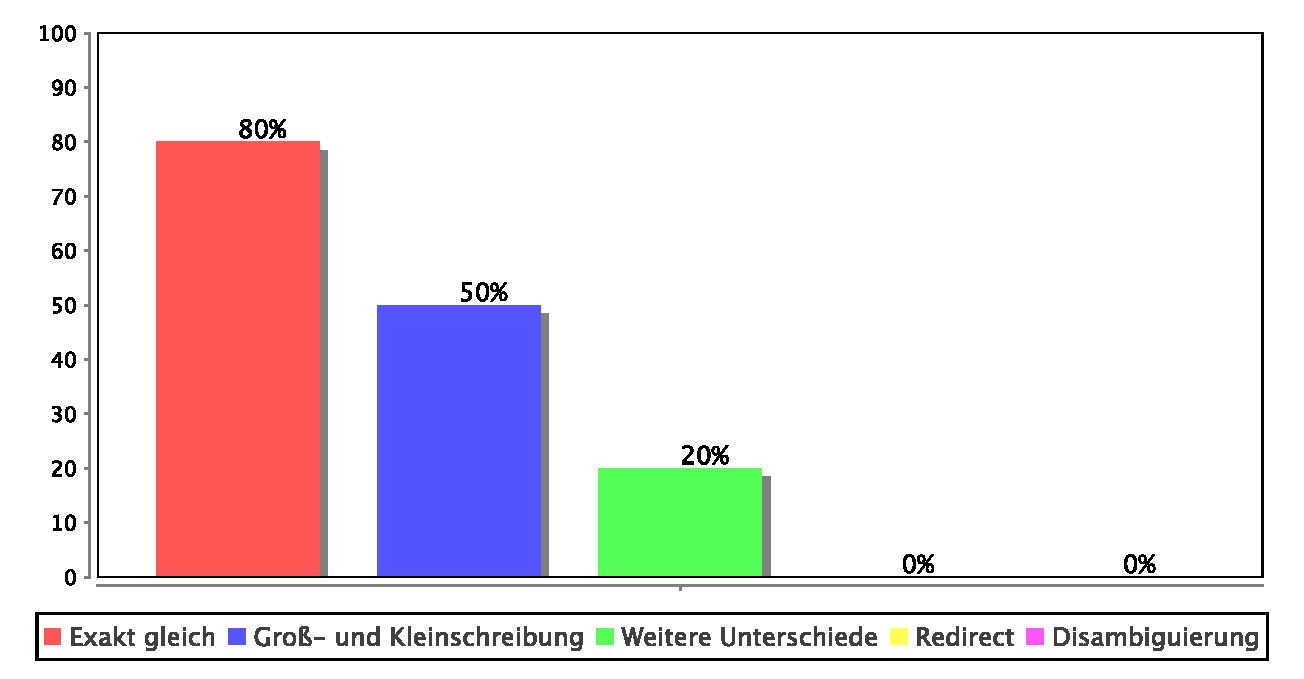
\includegraphics[width=\textwidth]{wortschatz2dbpedia/analyse/mapping1/stichprobe1/wortschatz2dbpedia.analyse.GeneralClassifier.barchart.eps}
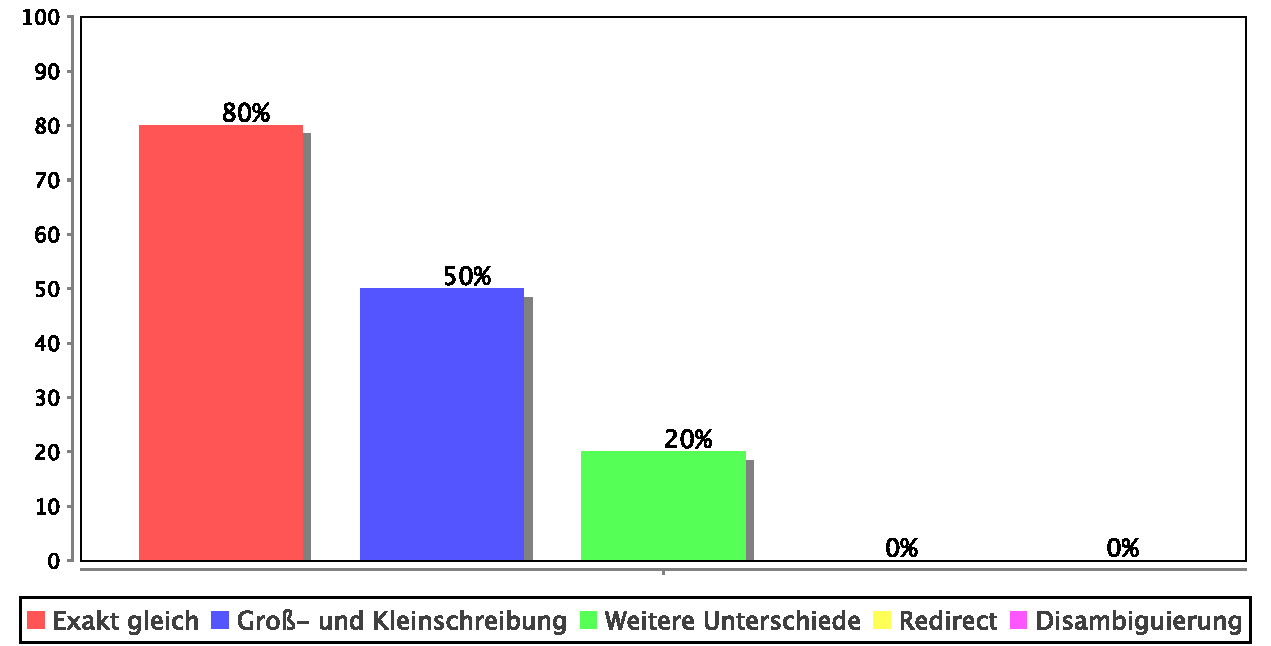
\includegraphics[width=\textwidth]{img/pdf/wortschatz2dbpedia.analyse.GeneralClassifier.barchart.pdf}

Zur Zeit der Analyse wurden Disambiguationsseiten und Redirects in der DBpedia noch nicht einheitlich behandelt.
Grundsätzliche Direktive bei der Extraktion von Artikeln aus der Wikipedia ist es, dass das Label der DBpedia-Ressource zu einem Artikel mit dessen Titel übereinstimmt.
Aus diesem Grund wird, um auch Disambiguierungsseiten (Seiten für mehrdeutige Begriffe, wie \zb{} \emph{Bank}) zu erkennen, der String "`(disambiguation)"' beim Matching ignoriert.
Dies erlaubt, dass auch ein Paar wie (\emph{Time\_(disambiguation)},\emph{Time}) gefunden wird. Zur Zeit der Erstellung des ersten Mappings wurde der String "`(disambiguation)"' jedoch in vielen Fällen 
bei der Extraktion der Wikipedia zur DBpedia entfernt. Die DBpedia-Ressource mit "`(disambiguation)"' im Titel existierte jedoch trotzdem noch, nur dass sie keinen Inhalt hatte.
Nachfragen ergaben jedoch, dass dies später behoben werden sollte, sodass am Matching nichts verändert, beim Betrachten der Stichproben Disambiguierungen jedoch außen vor gelassen werden.
Weiterhin existierten auch zu einigen Redirects DBpedia-Entitäten, die eigentlich in einem anderen Datenset sind. Da auch dies behoben werden sollte, werden auch die Redirects aus der Stichprobenbetrachtung
ausgeklammert.
%Einträge, die auf Disambiguierungsseiten (43 Einträge) oder Redirects (13 Einträge) verwiesen, waren deshalb fehlerhaft.
Von nun an werden nur die restlichen 144 Einträge betrachtet, die geschätzte Genauigkeit dieser Teilmenge beträgt $\valunit{59}{\%}$. Das $\valunit{95}{\%}$-Konfidenzintervall beträgt $[73,97]$,
also $[\valunit{50.6}{\%},\valunit{67.4}{\%}]$.
%\footnote{Linke Grenze abgerundet, Rechte Grenze aufgerundet auf zwei Stellen hinter dem Komma. Dies gilt für alle Konfidenzintervalle in dieser Arbeit.
%Alle anderen Werte sind auf zwei Nachkommastellen mathematisch (geodätisch) gerundet.}.
Im Folgenden wird die Zusammensetzung der Stichprobe und die Genauigkeit der einzelnen Teile genauer aufgeschlüsselt.
\subsection{Unterschiede in der Groß- und Kleinschreibung}

%Da Wikipediaartikeltitel immer mit einem Großbuchstaben anfangen, können folgende Fälle auftreten:
\iffalse
\begin{center}
\begin{tabular}{p{4cm}lll}
Unterschiede& \multicolumn{2}{l}{Beispiel} \\
\hline
keine				&Baird  	&Baird\\
erster Buchstabe\footnotemark	&Mandolin  	&mandolin\\
weitere Buchstaben		&AirPort  	&Airport\\
\hline
alles Andere			&Théodore 	&Theodore\\
\end{tabular}
\end{center}
\footnotetext{Da Wikipediaartikeltitel immer mit einem Großbuchstaben anfangen, handelt es sich in diesem Fall immer um ein kleingeschriebenes Wortschatzwort.}
\newpage
\fi
\subparagraph*{Häufigkeit}~\\
%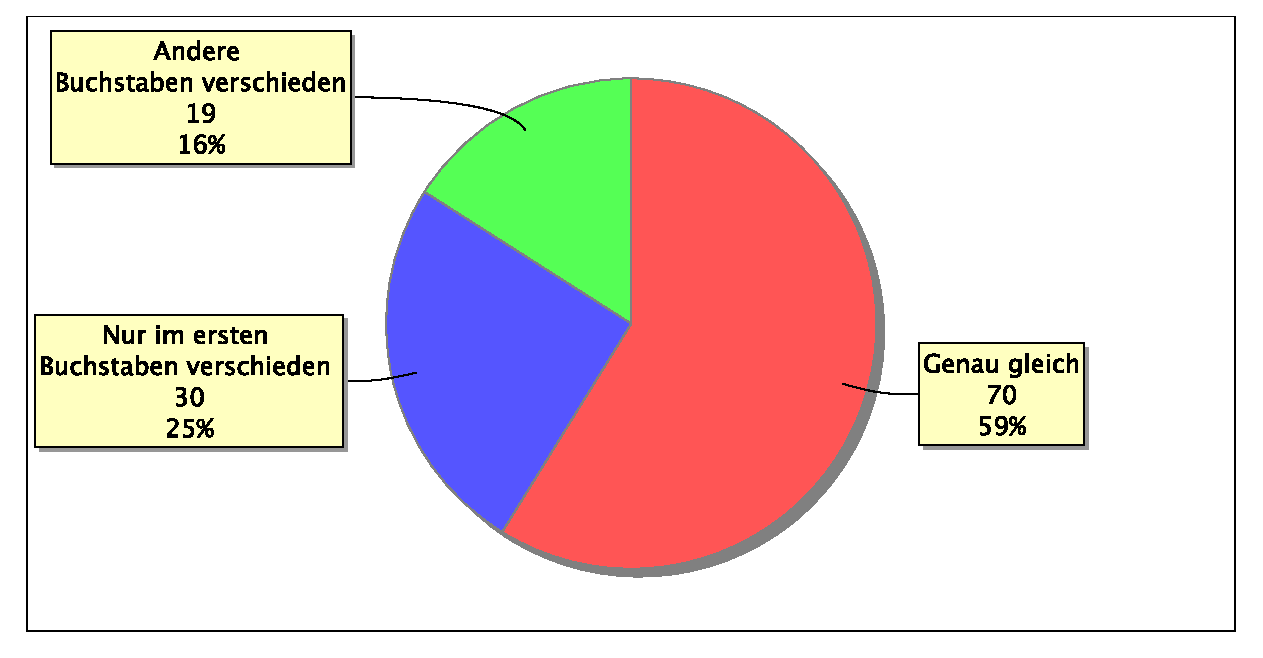
\includegraphics[width=\textwidth]{wortschatz2dbpedia/analyse/mapping1/stichprobe1/wortschatz2dbpedia.analyse.CaseClassifier.piechart.eps}
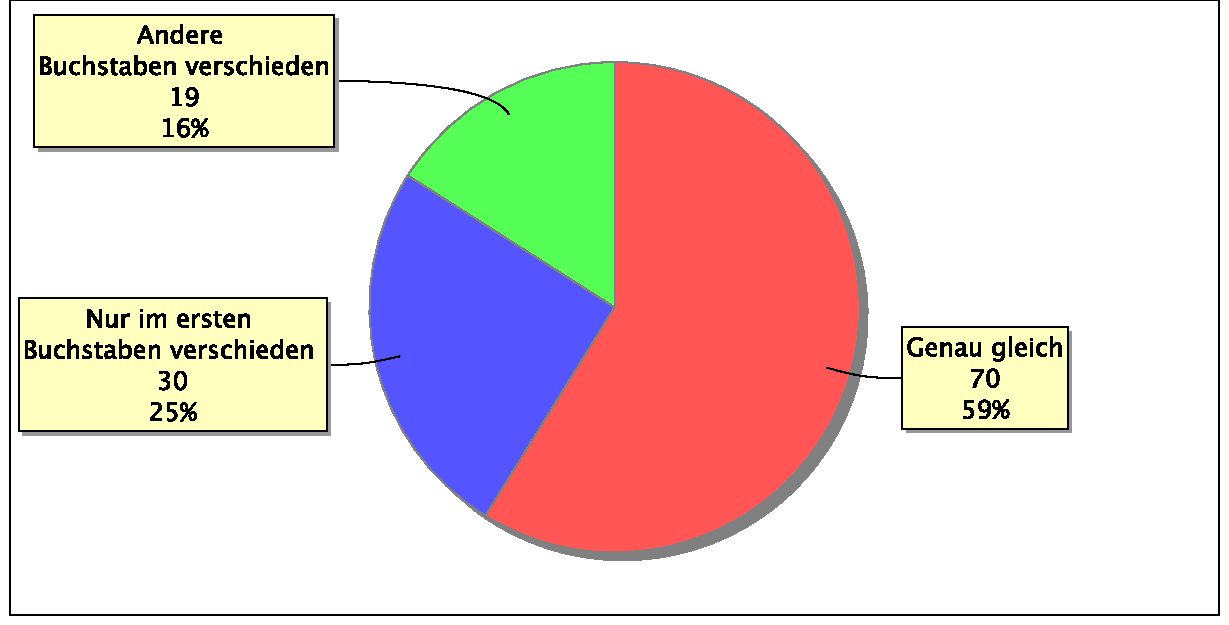
\includegraphics[width=\textwidth]{img/pdf/wortschatz2dbpedia.analyse.CaseClassifier.piechart.pdf}
\subparagraph*{Genauigkeit}~\\
%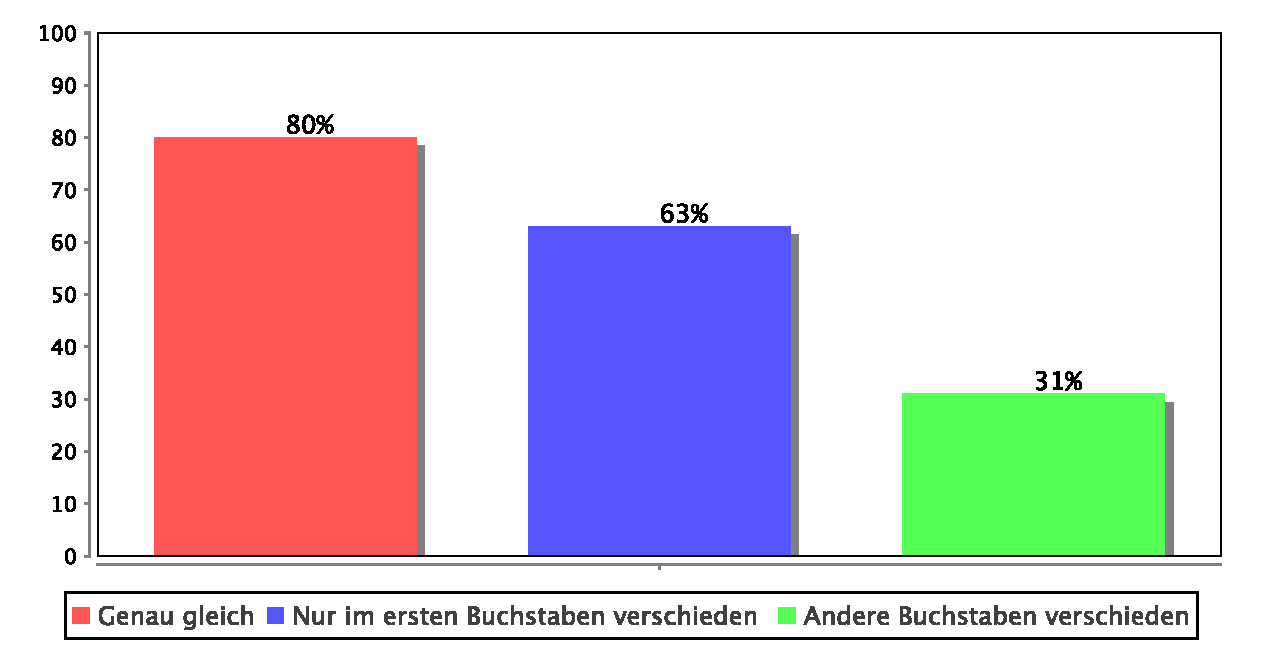
\includegraphics[width=\textwidth]{wortschatz2dbpedia/analyse/mapping1/stichprobe1/wortschatz2dbpedia.analyse.CaseClassifier.barchart.eps}
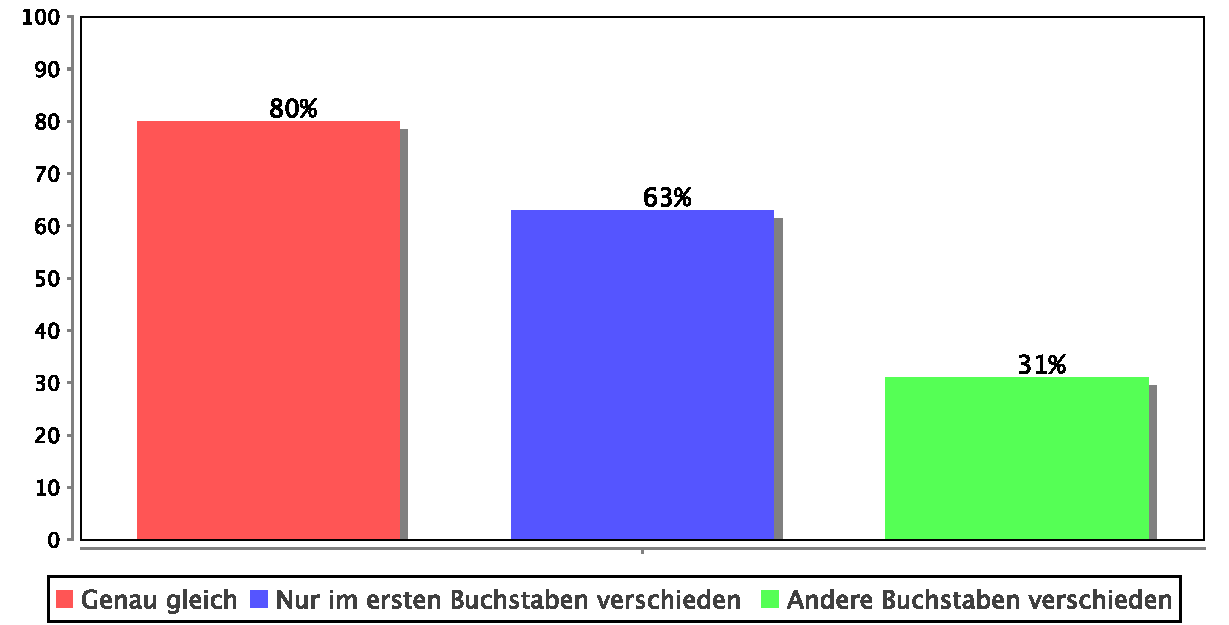
\includegraphics[width=\textwidth]{img/pdf/wortschatz2dbpedia.analyse.CaseClassifier.barchart.pdf}
Obwohl der Artikelname immer groß geschrieben und dessen eigentliche Großschreibung daher unbekannt ist,
gibt es eine deutliche Differenz zwischen der Genauigkeit von \valunit{80}{\%} bei groß geschriebenen und \valunit{63}{\%} bei klein geschriebenen Wörtern des Wortschatzes.
Dies wird damit erklärt, dass Wikipedia eher Artikel über spezielle Begriffe, also vor allem Eigennamen, enthält, die im englischen groß geschrieben werden.
Sucht man also zu einem beliebigen Wort aus dem Wortschatz ein passendes Gegenstück in der DBpedia, dann wird dieses Gegenstück mit einer höheren Wahrscheinlichkeit ein Eigenname und damit 
im normalen Sprachgebrauch groß geschrieben sein.
% Nach dem Erstellen dieser Analyse fiel auf, dass die Betrachtung der Groß- und Kleinschreibung anhand des Artikelnamens wenig aussagekräftig ist, da sowohl der Artikelname als 
% auch der Artikeltitel immer mit einem Großbuchstaben anfangen. Es kann also passieren, dass der DBpedia-Artikelname eigentlich klein geschrieben wird und somit ein klein geschriebenes Wort 
% aus dem Wortschatz fälschlicherweise als nicht exakt passend oder ein groß geschriebenes Wortschatzwort fälschlicherweise als exakt passend deklariert wird.

% In der Anforderungsanalyse in Abschnitt \ref{sec:anforderungen} wird eine Unterteilung in Korrespondenzen hoher und niedriger Präzision festgelegt.
% Beim Betrachten der Daten wird augenscheinlich, dass nur die exakten Übereinstimmungen über eine ausreichend hohe Präzision für den ersten Typen verfügen.
% Der Unterschied in der Genauigkeit zwischen den Wörtern, die im nur Ersten, und denen, die auch in anderen Buchstaben Unterschiede in der Großschreibung aufweisen, ist jedoch auch noch sehr groß.
 Die Präzision der Wörter mit beliebigen Unterschieden in der Großschreibung ist mit \valunit{31}{\%} selbst für eine unsichere Verknüpfungen zu niedrig.
% Lässt man den Nutzer im Wortschatz zwischen mehreren Alternativen wählen, so könnte so ein Link jedoch durchaus nützlich sein. Gegen eine Aufnahme dieser Paare sprechen dennoch folgende Gründe:
\iffalse
\begin{enumerate}
\item würde dadurch die immer noch gute Genauigkeit der anderen Verknüpfungen gemindert
\item würden bei einer Häufigkeit von \valunit{16}{\%} und einer Genauigkeit von \valunit{31}{\%} die hinzukommenden korrekten Paare nur \valunit{4.96}{\%} der Größe des bisherigen Mappings betragen
\item würde dann ein dritter Linktyp ("`ganz unsicher"') nötig werden, dies lohnt sich aufgrund der geringen Anzahl dieser Kategorie jedoch nicht und würde den Prozess nur unnötig verkomplizieren
\end{enumerate}
\fi
% \subparagraph{Schlußfolgerung}
% Um dieses Manko zu beheben, wird die Großschreibung des Begriffs bei DBpedia anhand des Abstracts ermittelt.
% Eine Liste sämtlicher Abstracts ist auf der Seite der DBpedia im Format N3 herunterladbar\footnote{\url{http://wiki.dbpedia.org/Downloads}}.
% Ist das Wort im Abstract überwiegend klein geschrieben, dann wird das Wort als klein geschrieben definiert.
% Anderenfalls (also auch bei Gleichstand und wenn es dort gar nicht vorkommt) wird es als groß geschrieben definiert.
% Vorkommen des Wortes am Satzanfang werden dabei ignoriert.

%Die exakten Matches werden als Links mit hoher Präzision aufgenommen, diejenigen, deren Groß- und Kleinschreibung sich unterscheidet als Links mit niedriger Präzision.
% Einträge mit Unterschieden in der Großschreibung über den ersten Buchstaben hinaus werden nicht aufgenommen.
%Da jedoch keine genaue Grenze für den zweiten Typen festgelegt wurde, fiel die Entscheidung schwer, ob 
%Im Vorhinein wurde keine bestimmte Grenze für die Genauigkeit festgelegt. Ist nur die Großschreibung des ersten Buchstabens verschieden, 
\subsection{Sonderzeichen}
Nach einer kurzen Sichtung der Stichprobe wurden die Wörter, die Sonderzeichen enthalten, in die folgenden Kategorien unterteilt:
\begin{center}
\begin{tabular}{p{4cm}lll}
\toprule
Kategorie& \multicolumn{2}{l}{Beispiel} \\
\midrule
Akzente und Umlaute		&\stichprobentabelleninneres{Théodore}  	&\stichprobentabelleninneres{Theodore}\\
~				&\stichprobentabelleninneres{Mädchen}		&\stichprobentabelleninneres{Madchen}\\
\midrule
Striche				&\stichprobentabelleninneres{Subcontractor}	&\stichprobentabelleninneres{sub-contractor}\\
~				&\stichprobentabelleninneres{MK801}		&\stichprobentabelleninneres{MK-801}\\
\midrule
Punkte				&\stichprobentabelleninneres{D.b.s.}		&\stichprobentabelleninneres{DBs}\\
				&\stichprobentabelleninneres{D.I.R.T.}		&\stichprobentabelleninneres{dirt}\\
				&\stichprobentabelleninneres{K.I.N.G.}		&\stichprobentabelleninneres{king}\\
\midrule
Mehrere davon			&\multicolumn{2}{c}{In der Stichprobe nicht vorhanden}\\
\midrule
Anderes				&\stichprobentabelleninneres{Cat}		&\stichprobentabelleninneres{\`cat}\\
~				&\stichprobentabelleninneres{Waryś}		&\stichprobentabelleninneres{WARY}\\
~				&\stichprobentabelleninneres{Jihâd}		&\stichprobentabelleninneres{`jihad}\\
~				&\stichprobentabelleninneres{Mârşa}		&\stichprobentabelleninneres{Mara}\\
\bottomrule
\end{tabular}
\end{center}

\subparagraph{Häufigkeit}~\\
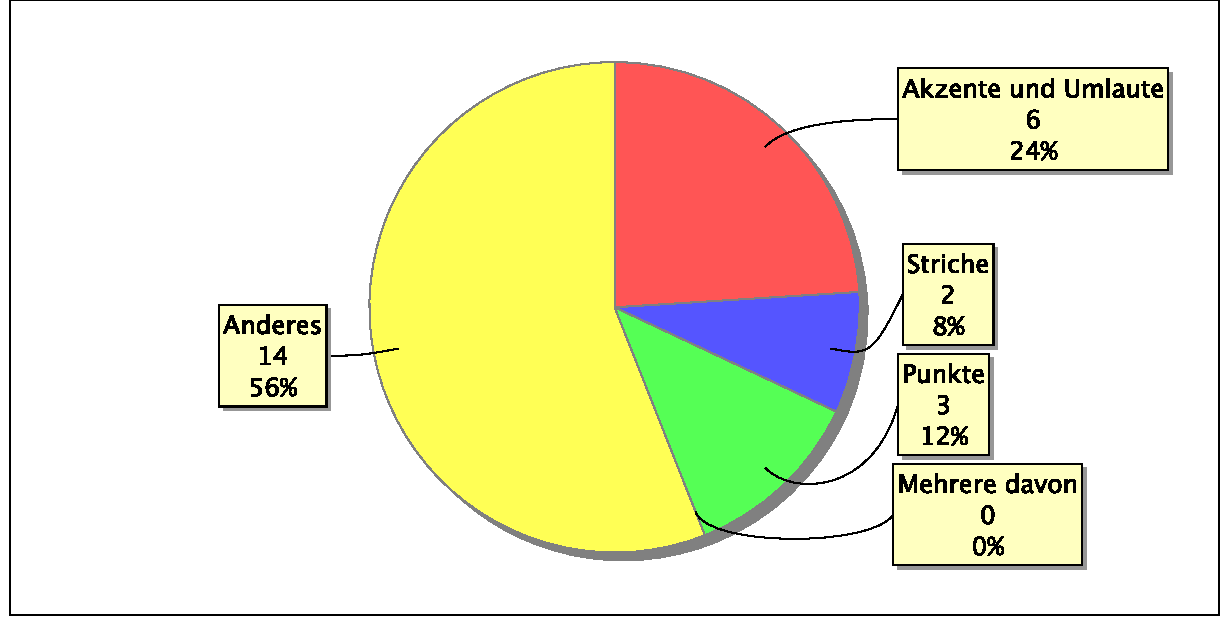
\includegraphics[width=\textwidth]{img/pdf/wortschatz2dbpedia.analyse.SpecialCharactersClassifier.piechart.pdf}
\subparagraph{Genauigkeit}~\\
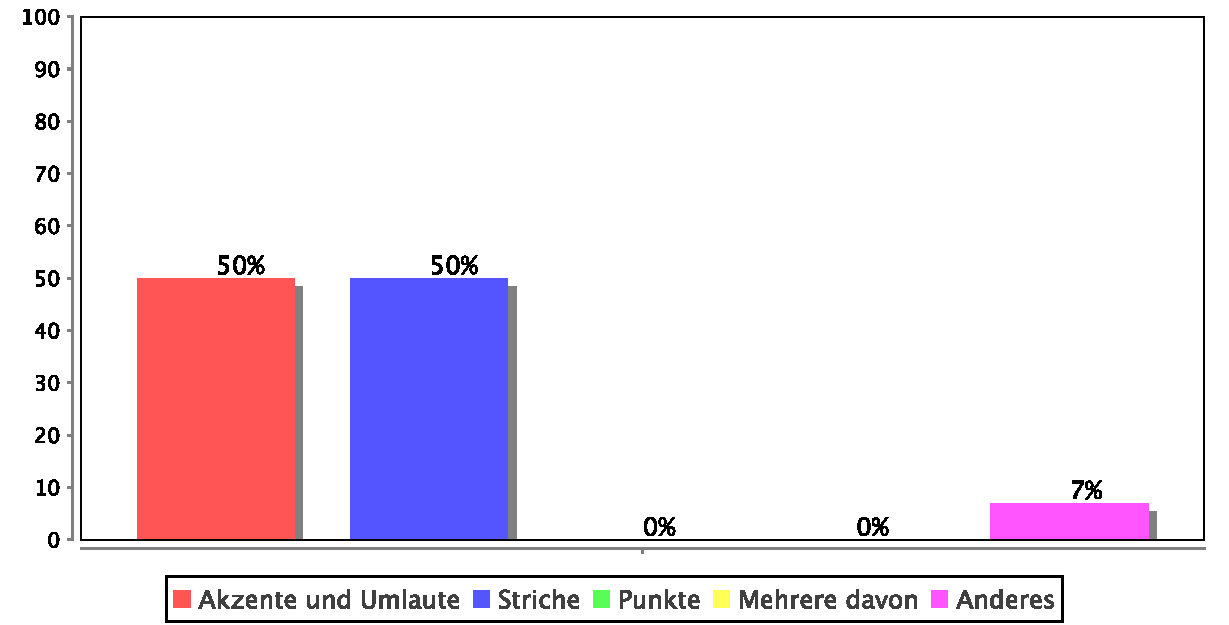
\includegraphics[width=\textwidth]{img/pdf/wortschatz2dbpedia.analyse.SpecialCharactersClassifier.barchart.pdf}
\paragraph{Erweiterte Stichprobe}
Aufgrund der geringen Stichprobenteilgröße ist die Aussagekraft der Einschätzung sehr gering. Außerdem wird bei der Betrachtung der Sonderzeichen in der ersten Stichprobe die Großschreibung ignoriert.
Aus diesem Grund wurde für die drei Kategorien "`\emph{Akzente und Umlaute}"', "`\emph{Striche}"' und "`\emph{Punkte}"' noch je eine weitere zufällige Stichprobe im Umfang von 30 Einträgen untersucht,
bei der nur die Großschreibung des ersten Buchstabens ignoriert wird.
\subparagraph{Akzente und Umlaute}
\begin{table}[h]
\caption{Umwandlungstabelle der Umlaute}
\begin{tabular}{l|l}
\toprule
ÌÍÎÏ		&I\\
ÀÁÂÃÄÅÆ		&A\\
Ç		&C\\
ÈÉÊË		&E\\
Ý		&Y\\
ÙÚÛÜ		&U\\
ÒÓÔÕÖ		&O\\
ìíîï		&i\\
àáâãäåæ		&a\\
ç		&c\\
èéêë		&e\\
ý		&y\\
ùúûü		&u\\
òóôõö		&o\\
\bottomrule
\end{tabular}
\end{table}
%\clearpage%damit die tabelle nicht sonstwo platziert wird (klappt aber auch nicht immer)
%\subparagraph*{Ergebnis}
25 der 30 Einträge sind gültig (keine redirects), Fünf davon korrekt. Die Genauigkeit beträgt also \valunit{20}{\%}, das \valunit{95}{\%}-Konfidenzintervall liegt bei [1,9] $(\valunit{4}{\%},\valunit{36}{\%})$.
\subparagraph{Striche}
23 der 30 Einträge sind gültig, Sieben davon korrekt. Die Genauigkeit beträgt \valunit{30.43}{\%}, das \valunit{95}{\%}-Konfidenzintervall liegt bei [3,11] $(\valunit{13.03}{\%},\valunit{47.83}{\%})$.
\subparagraph{Punkte}
24 der 30 Einträge sind gültig, Einer davon korrekt. Die Genauigkeit beträgt \valunit{4.17}{\%}, das \valunit{95}{\%}-Konfidenzintervall liegt bei [0,3] $(\valunit{0}{\%},\valunit{12.5}{\%})$.
%\subparagraph{Schlußfolgerung}
%Zu klein ist die Genauigkeit der drei Kategorien. Auf eine Aufnahme von Einträgen, die sich in Sonderzeichen unterscheiden wurde also verzichtet.
\subsection{Mapping 1}\label{sec:mapping1}
Die folgenden Parameter wurden aus der Analyse der ersten Stichprobe für ein neues Mapping, Mapping 1, festgelegt:
\begin{itemize}
\item Es werden weiterhin nur DBpedia-Ressourcen und Wortschatzwörter mit einer Länge von mindestens drei Buchstaben in Betracht gezogen.\footnotemark
\footnotetext{Die meisten Wörter der englischen Sprache, zu denen es Artikel in der Wikipedia gibt, haben eine Länge von mindestens drei Buchstaben,
denn die Artikel behandeln selten Verben und Präpositionen, wie \emph{to} und \emph{in}, sondern fast ausschließlich Eigennamen, Objekte und abstrakte Konzepte)}
\item Disambiguierungsmarker werden weiterhin ignoriert (\emph{x\_(disambiguation)} wird also weiterhin wie \emph{x}) behandelt. In das Mapping wird jedoch nicht dieses Paar aufgenommen sondern
die Menge aller Paare $(a,x)$, wobei der Artikel mit dem Namen $a$ eine der Disambiguierungsmöglichkeiten von $x$ ist. Diese Paare werden als unsichere Korrespondenzen aufgenommen.
\item Identische Paare werden als Links mit hoher Präzision definiert. Ist der Artikel ein Redirect, dann wird der Artikelname durch den des Ziels des Redirects ersetzt.
\item Paare, bei denen sich einzig die Großschreibung des ersten Zeichens unterscheidet, werden als unsichere Korrespondenzen aufgenommen.
\item Weitere Paare werden nicht aufgenommen.\footnotemark
\footnotetext{Das mag nach solch einer ausführlichen Analyse etwas enttäuschend anmuten aber weniger ist manchmal mehr.}
\end{itemize}
Die Großschreibung des Artikelnamens wird jedoch nicht mehr als immer groß angenommen, sondern anhand des Abstracts der DBpedia-Entität ermittelt.
Eine Liste sämtlicher Abstracts ist auf der Seite der DBpedia im Format N3 herunterladbar\footnote{\url{http://wiki.dbpedia.org/Downloads}}.
Ist das Wort im Abstract überwiegend klein geschrieben, dann wird das Wort als klein geschrieben definiert.
Anderenfalls (also auch bei Gleichstand und wenn es dort gar nicht vorkommt) wird es als groß geschrieben definiert.
Vorkommen des Wortes am Satzanfang werden dabei ignoriert.

\iffalse
\subsection{Erweiterung zur Groß- und Kleinschreibung}
Nach dem Erstellen dieser Analyse fiel auf, dass die Betrachtung der Groß- und Kleinschreibung anhand des Artikelnamens wenig aussagekräftig ist, da sowohl der Artikelname als 
auch der Artikeltitel immer mit einem Großbuchstaben anfangen. Es kann also passieren, dass der DBpedia-Artikelname eigentlich klein geschrieben wird und somit ein klein geschriebenes Wort 
aus dem Wortschatz fälschlicherweise als nicht exakt passend oder ein groß geschriebenes Wortschatzwort fälschlicherweise als exakt passend deklariert wird.
Interessant ist hier, dass trotzdem ein signifikanter Unterschied hinsichtlich der Genauigkeit besteht (\valunit{80}{\%} bei groß geschriebenen, \valunit{63}{\%} bei klein geschriebenen Wörtern aus dem Wortschatz).
Dies wird damit erklärt, dass Wikipedia eher Artikel über spezielle Begriffe, also vor allem Eigennamen, enthält, die im englischen groß geschrieben werden.
Sucht man also zu einem beliebigen Wort aus dem Wortschatz ein passendes Gegenstück in der DBpedia, dann wird dieses Gegenstück mit einer höheren Wahrscheinlichkeit ein Eigenname und damit 
im normalen Sprachgebrauch groß geschrieben sein.

\begin{rem}
Die Analyse muss streng genommen für jede Sprache wiederholt werden. Aus diesem Grunde wurden hier die einzelnen Schritte auch detailliert und nachvollziehbar aufgeführt.
\end{rem}
\fi
\chapter{Wortsinndisambiguierung}\label{sec:disambiguierung}
In diesem Kapitel wird die Entwicklung des NLP2RDF-Moduls für die Wortsinndisambiguierung beschrieben, das auf dem Mapping von Wortschatz2DBpedia aus Abschnitt \ref{sec:wortschatz2dbpedia} aufbaut.
Das Verfahren nutzt aus, dass die in einem Text referenzierten Konzepte einen gemeinsamen Sinnzusammenhang haben.
Als Annäherung an eine Messung dieses Sinnzusammenhanges der möglichen Bedeutungen werden sowohl statistische als auch semantische Ähnlichkeitsmaße eingeführt, deren Maximierung mit hoher Wahrscheinlichkeit
die tatsächlich gemeinten Bedeutungen liefert.

%\paragraph{Definition}
\begin{dfn}
Der Begriff \emph{Wortsinndisambiguierung} (den auch nur \emph{Disambiguierung} oder \emph{WSD}) bezeichnet die Zuordnung einer Bedeutung, also eines Sinnes, aus einem \emph{Wortsinninventar} zu einem gegebenen Wort in einem bestimmten Text, wobei dieses Wort potentiell mehrere Bedeutungen besitzt.
Diese Aufgabe umfasst daher zwei Schritte:
\begin{enumerate}
 \item die Bestimmung aller möglichen verschiedenen Bedeutungen dieses Wortes
 \item ein Verfahren, um jedem Vorkommen dieses Wortes seine passende Bedeutung zuzuweisen
\end{enumerate}
Diese Definition wurde frei übersetzt aus \citet{wsd-stateoftheart}.
\end{dfn}

\begin{dfn}
Ein Ähnlichkeitsmaß ist eine Funktion, die einem Paar von Objekten eine Zahl aus dem reellen Intervall $[0, 1]$ zuordnet. Dabei korrespondiert der
Wert 1 zur maximalen Ähnlichkeit und der Wert 0 zur maximalen Unähnlichkeit \citep[][Seite 215]{aehnlichkeitssuche}.
\end{dfn}

%Die automatische Disambiguierung eines Wortsinnes ist aus zweierlei Gründen relevant für NLP2RDF:
\iffalse
\begin{enumerate}
\item wird durch den neuartigen Ansatz der Kombination einer NLP-Pipeline\footnote{bzw. einer komplexeren Struktur als einer Pipeline, welche zum Zeitpunkt der Diplomarbeit als Verbesserung angedacht war}
mit einem Lernalgorithmus ein neues Verfahren zur Disambiguierung vorstellbar
\item besteht die Erwartung, dass eine Disambiguierung die Leistung des Lernalgorithmus' verbessert
\end{enumerate}
In diesem Kapitel werden nun beide dieser Ansätze diskutiert und evaluiert.
\fi
%\section{WSD zur Performancesteigerung}
\section{Motivation}
Eines der Ziele von NLP2RDF ist die Featureextraktion aus natürlichsprachigen Texten mithilfe des Einsatzes eines Lernalgorithmus mit Eingabe des mehrfach angereicherten Textes
(siehe Abschnitt \ref{sec:tiger_corpus_navigator}, \emph{TIGER Corpus Navigator}).
Eine dieser Anreicherungen wird durch das Modul \emph{Wortschatz2DBpedia} vorgenommen, welches zu jedem Substantiv des Textes eine Menge von Kandidaten für mögliche Bedeutungen dieses Wortes in Form der
diese Bedeutungen beschreibenden Wikipedia/DBpedia-Artikel an dieses Substantiv anhängt.
Für das Erlernen von semantischen Features ist es erwartungsgemäß ein großer Vorteil, wenn diese Menge an Bedeutungen auf genau die gemeinte Bedeutung des Wortes eingegrenzt werden kann.

% Zwei Gründe sprechen nun für eine Disambiguierung:
% \begin{enumerate}
%  \item der erste Schritt, also die Bestimmung aller möglichen verschiedenen Bedeutungen dieses Wortes ist bereits erfolgt
%  \item es ist zu erwarten, dass der Lernalgorithmus eine höhere Leistung erbringt, wenn er weniger irreführende Information verarbeiten muss
% \end{enumerate}
\paragraph{}
Folgenden Typen von Verfahren wurden dabei in Erwägung gezogen:
\begin{enumerate}
 \item "`Häufigste Bedeutung"'
 \item Integration eines bereits existierenden Verfahrens
 \item Neuentwicklung eines Verfahrens
\end{enumerate}

\paragraph{"`Häufigste Bedeutung"'}
Bei diesem Verfahren wird, egal wie der Kontext des Wortes aussieht, für jedes Wort immer dieselbe Bedeutung gewählt, nämlich diejenige mit der größten Häufigkeit im normalen schriftlichen Gebrauch.\footnotemark{}
\footnotetext{In der Praxis wird, um eine Messung zu ermöglichen, die Häufigkeit anhand eines Referenzkorpus bestimmt.}
Trotz seiner Einfachheit erreichte dieses Verfahren eine Präzision von \valunit{57}{\%} im englischen Test von Senseval-1 \citep{wsd-survey}.\footnotemark{}
\footnotetext{Eine andere Sichtweise ist jedoch, dass gerade die selten vorkommenden Bedeutungen von besonderer Wichtigkeit und deshalb stärker zu gewichten sind. Dies würde sich jedoch auch auf die 
Bewertung der anderen Verfahren auswirken.}
Die Zuordnung eines Wort zu einer Bedeutung kann vorberechnet und damit schnell abgerufen werden und das Verfahren ist sehr simpel zu implementieren.
Allerdings benötigt man ein Referenzkorpus, bei dem für jedes Substantiv ausreichend viele Beispielsätze vorhanden sind, deren Bedeutungen in Form von Wikipedia-Artikelnamen gekennzeichnet sind.

\paragraph{Integration eines bereits existierenden Verfahrens}
Wortsinndisambiguierung ist ein sehr populäres Forschungsgebiet. Ein ausführlicher Überblick findet sich in \cite{wsd-stateoftheart}.Aus diesem Grund existieren bereits eine große Menge an Verfahren, die entweder in spezielle Software (\zb{} Übersetzungsprogramme) integriert
oder als eigenständige Programme implementiert sind. Aufgrund der Wichtigkeit von Disambiguierungsverfahren für die natürliche Sprachverarbeitung existiert sogar eine internationale Organisation
namens \emph{Senseval}, die sich ausschließlich mit der Evaluation von Wortsinndisambiguierungssystemen befasst.
Leider basieren die meisten dieser Systeme auf Wordnet-Synsets und nicht auf Wikipedia-Artikeln.
Eine der Ausnahmen war jedoch ein System von \citet{cucerzan2007} was gute Ergebnisse lieferte.
Leider gelang es nicht, den Autor zu erreichen und das Paper gibt keine weiteren Informationen, ob eine Implementierung des dort vorgeschlagenen Systems existiert und wenn ja, ob sie frei verfügbar ist.

\paragraph{Neuentwicklung eines Verfahrens}
%Es war zwar nicht zu erwarten, dass eine Eigenentwicklung bereits etablierte Verfahren übertreffen würde aber da der Autor von \cite{cucerzan2007} nicht zu erreichen war und da eine Implementierung des dort
%vorgeschlagenen Systems sehr umfangreich wäre, wurde eine simple Eigenentwicklung vorgenommen.

Der Vorteil der Neuentwicklung eines Verfahrens liegt darin, dass man es optimal an die Erfordernisse und vorhandenen Daten von NLP2RDF anpassen kann.
Durch die Vielzahl an bereits vorhandenen Modulen ist eine große Menge an für eine Disambiguierung hilfreicher Information verfügbar.
Insbesondere das Mapping von Wortschatzdaten auf DBpedia, das vom Unterprojekt \emph{Wortschatz2DBpedia} erzeugt wird, ermöglicht bereits eine qualitativ hochwertige\footnotemark{} Zuordnung von Wörtern zu ihren möglichen Bedeutungen.
\footnotetext{\emph{Wortschatz2DBpedia} wurde für das Paper \cite{triplify_challenge_2009_paper} der 3. Preis bei der LOD Triplification Challenge 2009 \cite{triplify_challenge_2009_website} verliehen.}
Weiterhin erlaubt eine modulare Bauweise eine einfache Anpassung an verschiedene Wortsinninventare. So können auch Artikel aus einem speziellen Fachgebiet mit einer eigenen Ontologie disambiguiert werden.

Diese Gründe führten zur Neuentwicklung eines Disambiguierungsverfahrens.
Im Folgenden wird das verwendete Prinzip erläutert.
\section{Einleitung}
Die Wörter eines Satzes werden durch die Verben miteinander in Beziehung gesetzt.
Die Art der Beziehung wird hier jedoch vernachlässigt und nur die Substantive werden betrachtet, da nur zu diesen normalerweise Wikipedia-Artikel existieren.\footnotemark{}
\footnotetext{Dies ist eine wesentliche Einschränkung, ein Satz wie "`Er saß auf einer Bank."' ist damit nicht zu disambiguieren.
%Aus Gründen der Einfachheit wurde sie trotzdem beibehalten. Mögliche Lösungen dieses Problems werden später diskutiert.\todo{referenz setzen? oder aus footnote rausnehmen?}
}
Aus der Menge der Substantive des Textes ist jedoch auch eine wichtige Information zu entnehmen.
Einander ähnliche Konzepte werden nämlich tendenziell häufiger in Beziehung gebracht als Wörter komplett verschiedener Domänen, außerdem hat ein Wort meist im gesamten Text die gleiche Bedeutung \citep{one_sense_per_discurse}.
Wählen wir also die Bedeutungen aus, die etwas miteinander zu tun haben, dann ist unsere Entscheidung mit einer höheren Wahrscheinlichkeit korrekt, als wenn wir Bedeutungen wählen, die in gar keiner Relation zueinander stehen.

\paragraph{Beziehungsstärke versus Ähnlichkeit}
Ob und in welchem Grad ein Konzept mit einem anderen in einer Beziehung steht ist schwer festzustellen und zu quantifizieren.
Eine grundlegende Hypothese der meisten hier genutzten Maße ist, dass sich die Beziehungsstärke zwischen zwei Konzepten durch ihre Ähnlichkeit approximieren lässt.
Wenn zwei Konzepte einander ähnlich sind, stehen sie natürlich auch in einer Beziehung zueinander, umgekehrt müssen zwei Konzepte, die einander ähnlich sind jedoch nicht zwangsläufig auch verwandt sein.
Deshalb werden in diesem Kapitel Maße sowohl für die Ähnlichkeit als auch für die Beziehungsstärke eingeführt.
%Zu prüfen ist also, in wieweit das Verwenden verschiedener Ähnlichkeitsfunktionen eine hochwertige Disambiguierung ermöglicht.
\begin{figure*}[h]
\begin{center}%COn{dl}
\Tree[2]{
			&\K{Auto}\GB{dl}{<-}\GB{dr}{<-}\\
\K{Opel Astra}		&					&\K{Skoda Fabia}\\
} 
\end{center}
%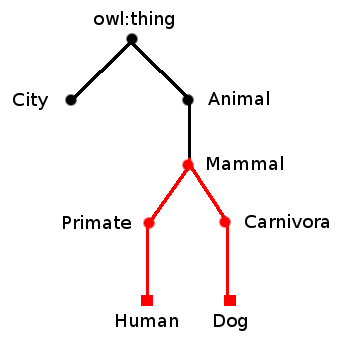
\includegraphics[width=0.5\textwidth]{img/hierarchy_with_classes.png} 
\caption{Die Konzepte \emph{Opel Astra} und \emph{Skoda Fabia} sind einander \emph{ähnlich}, da beide Instanzen der Klasse \emph{Auto} sind.}
\label{fig:disambiguierung_aehnlichkeit}
\end{figure*}

\begin{figure*}[h]
\begin{center}%COn{dl}
\Tree[2]{
			&\K{Kirche}\B{dl}_{\textnormal{steht in}}\B{dr}^{\textnormal{ Arbeitgeber von}} \\\
\K{Dorf}		&					&\K{Pfarrer}\\
} 
\end{center}
%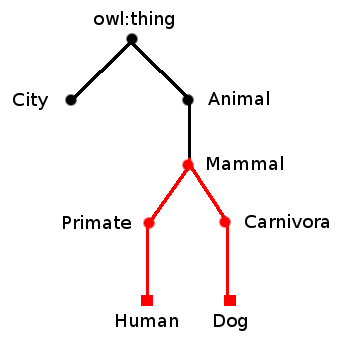
\includegraphics[width=0.5\textwidth]{img/hierarchy_with_classes.png} 
\caption{Die Konzepte \emph{Kirche}, \emph{Dorf} und \emph{Pfarrer} stehen in Beziehung zu einander, sind jedoch nicht ähnlich.}
\label{fig:disambiguierung_beziehungsstaerke}
\end{figure*}

\FloatBarrier
%Dies wird am besten deutlich an einem:
%Von jedem Wort dieses Textes wird das Lemma, auch Grundform genannt, bestimmt. Im Englischen geschieht dies mit dem Porter-Stemmer-Algorithmus.

\begin{bsp}
"`The enterprise is in space."'\\
~\\
Die beiden Substantive des Satzes sind \emph{enterprise} und \emph{space}.
Da die passenden DBpedia-Artikel \emph{Enterprise} und \emph{Space} Disambiguierungsseiten sind, weist das Wortschatz2DBpedia-Mapping beiden Wörtern eine Fülle von möglichen Bedeutungen zu (nämlich unter anderem die Menge der 
auf diesen Seiten vorhandenen Disambiguierungslinks).
Aufgabe ist es nun, jedem der Substantive genau eine Bedeutung zuzuordnen.

~\\
Ein Ausschnitt der möglichen Bedeutungen:
%\emph{Enterprise} : \emph{Business}, \emph{Enterprise,_Florida}, \emph{Starship_Enterprise}
%\emph{Space} :  \emph{Whitespace}, \emph{Outer_space}, \emph{Personal_space}
\begin{center}
\begin{tabular}{ll}
\toprule
Enterprise&		Space\\
\midrule
Business&		Whitespace\\
Enterprise,\_Florida&	Outer\_space\\
Starship\_Enterprise&	Personal\_space\\
\bottomrule
\end{tabular}
\end{center}

\end{bsp}

%Dies setzt voraus, dass sich diese Wörter überhaupt 
Wir suchen uns also aus den Mengen der möglichen Bedeutungen der Substantive jene heraus, welches die gesamte Ähnlichkeit der gewählten Konzepte untereinander maximieren.
Formell ist die Aufgabe, ein passendes Ähnlichkeitsmaß s zu finden, wobei gilt:
\begin{equation*}s: \textnormal{Konzepte}^2 \rightarrow \setR\end{equation*}

Das Paar von Bedeutungen, welches dieses Änderungsmaß maximiert ist das Wahrscheinlichste und wird von der Disambiguierung als Resultat zurückgegeben.

%\subparagraph{Ein fiktives Ähnlichkeitsmaß}
 
\begin{center}
\begin{table}[H]
\begin{tabular}{lr}
\toprule
Bedeutungspaar $b$				&s($b_1$,$b_2$)\\
\midrule
(Business, Whitespace)				&\val{0.30}\\
(Business, Outer\_space)			&\val{0.02}\\
(Business, Personal\_space)			&\val{0.20}\\
(Enterprise,\_Florida, Whitespace)		&\val{0.06}\\
(Enterprise,\_Florida, Outer\_space)		&\val{0.01}\\
(Enterprise,\_Florida, Personal\_space)		&\val{0.10}\\
(Starship\_Enterprise, Whitespace)		&\val{0.05}\\
\textbf{(Starship\_Enterprise, Outer\_space)}	&\textbf{\val{0.70}}\\
(Starship\_Enterprise, Personal\_space)		&\val{0.03}\\
\bottomrule
\end{tabular}
\caption{Ein fiktives Ähnlichkeitsmaß. In diesem Fall maximiert das Paar \textbf{(Starship\_Enterprise, Outer\_space)} das Ähnlichkeitsmaß und die Disambiguierung gibt genau diese Bedeutungen zurück.}
\label{tab:beispiel-aehnlichkeitsmass}
\end{table}
\end{center}

%\paragraph{\todo{Vom Beispiel zur Allgemeinheit oder was auch immer}}
Dieses einfache Beispiel beinhaltet nur zwei Substantive. Selbstverständlich weisen viele Sätze mehr als Zwei auf. Weiterhin könnte eine Betrachtung eines weiteren Kontextes (also des gesamten Textes und nicht
nur des einzelnen Satzes) eine Verbesserung der Disambiguierungsleistung hervorrufen.
Um die Disambiguierung auch für mehr als zwei Substantive durchzuführen, gibt es zwei Möglichkeiten:

\begin{enumerate}
 \item Die Einführung eines Ähnlichkeitsmaßes s, das mehrstellig ist, beziehungsweise auf Tupeln oder Mengen beliebiger Größe arbeitet
 \item Die Definition einer Funktion h$: \pow{\setR} \rightarrow \setR$ wobei h eine Menge von Ähnlichkeitswerten aggregiert, also aus einer Menge von Ähnlichkeitswerten einen Gesamtähnlichkeitswert berechnet.
\end{enumerate}

Aufgrund der Komplexität eines mehrstelligen Ähnlichkeitsmaßes wird im Folgenden von der zweiten Option ausgegangen.
Dabei sei h "`monoton steigend"' im folgenden Sinne:
\begin{tabbing}
und \=\kill
Sei \>$M_1 = \{m_1,\ldots,m_{i-1},m_{i},m_{i+1},\ldots,m_n\}$\\
und \>$M_2 = \{m_1,\ldots,m_{i-1},m_{i'},m_{i+1},\ldots,m_n\}$, mit $m_{i'}>m_{i}$\\
\end{tabbing}
dann gilt: $\h(M_2) \geq \h(M_1)$.


\section{Problemstellung und Lösungsansatz}
Sei $K$ die Menge aller Konzepte, seien $w_1$, \ldots, $w_n$ die betrachteten Wörter (Substantive) des Textes, sei $K_i$ die Menge der möglichen Bedeutungen des Wortes $w_i$,
$b$ eine Bedeutungsauswahl, s ein Ähnlichkeitsmaß und h die Funktion, die die Ähnlichkeitswerte aggregiert also den Gesamtähnlichkeitswert berechnet.

Das zu lösende Disambiguierungsproblem lässt sich nun als Optimierungsproblem darstellen:
\begin{equation*}
\max_{b\in K_1\times\cdots\times K_n} \h\left(\bigcup_{(i,j) \in \{1,\ldots,n\}^2, i\neq j} s(b_i,b_j)\right)
\end{equation*}

\iffalse
\begin{equation*}
\max_{b\in K_1\times\cdots\times K_n} \sum_{(i,j) \in \{1,\ldots,n\}^2, i\neq j} s(b_i,b_j)
\end{equation*}
\fi

Da die semantische Beziehung zwischen Konzepten innerhalb eines Satzes tendenziell stärker ist als die von Konzepten verschiedener Sätze,
verspricht eine Gewichtung der Konzeptpaare eine höhere Erfolgsrate.
Sei $\g: \setN \rightarrow \setR$ nun eine monoton fallende Funktion, welche die erwartete Beziehungsstärke zwischen zwei Konzepten anhand ihrer Entfernung $d$ in Sätzen im Text berechnet,
$0 \leq \g(d) \leq 1$.

%\sout{Sei $\g: \setN^2 \rightarrow \setR$ nun eine Funktion, welche die erwartete Beziehungsstärke zwischen zwei Konzepten anhand ihrer Entfernung im Text berechnet.
%g ordnet dabei jedem Paar $(d_s,d_w)$, wobei $d_s$ die Entfernung in Sätzen und $d_w$ die Entfernung in Wörtern angibt, eine Gewichtung zu.
%Sei g weiterhin monoton fallend (im gleichen Sinne wie h monoton steigend ist).}
Dann erweitert sich das Problem zu:
\begin{equation*}
%\max_{b\in K_1\times\cdots\times K_n} \sum_{(i,j) \in \{1,\ldots,n\}^2, i\neq j} s(b_i,b_j) \cdot \textnormal{g}(d_s(w_i,w_j),d_w(w_i,w_j))
%\max_{b\in K_1\times\cdots\times K_n} h(\bigcup_{(i,j) \in \{1,\ldots,n\}^2, i\neq j} s(b_i,b_j) \cdot \textnormal{g}(d_s(w_i,w_j),d_w(w_i,w_j)))
\max_{b\in K_1\times\cdots\times K_n} \h\left(\bigcup_{(i,j) \in \{1,\ldots,n\}^2, i\neq j} s(b_i,b_j) \cdot \textnormal{g}(d_{ij})\right)
\end{equation*}
Als Gewichtungsfunktion g wird eine Exponentialfunktion $\g(d): d\rightarrow a^d$ verwendet mit $0<a\leq1$, sowie als Gesamtähnlichkeitsfunktion h die Summenfunktion.
Dies ergibt:
\begin{equation*}
\max_{b\in K_1\times\cdots\times K_n} \sum_{(i,j) \in \{1,\ldots,n\}^2, i\neq j} \left(s(b_i,b_j) \cdot a^{d_{ij}}\right)
\end{equation*}

%Im einfachsten Fall ist h die Summe.

\paragraph{Laufzeitkomplexität}
Da es $|K_1|\times\cdots\times |K_n|$ verschiedene Bedeutungsauswahlen gibt, ist der Algorithmus in dieser Form offensichtlich exponentiell in der Anzahl der im Text enthaltenen zu disambiguierenden Wörter
und damit nicht effizient.
Eine drastische Reduzierung der betrachteten Bedeutungsauswahlen durch eine Heuristik ist also erforderlich.
Die Charakteristika der Verfahren wurden aus \cite{global-optimization-algorithms} entnommen.
\subsection{Betrachtete Heuristische Optimierungsverfahren}
%In Frage kommen etwa:
\iffalse
 \begin{enumerate}
  \item Hill Climbing
  \item Simulierte Abkühlung
  \item Genetische Algorithmen
 \end{enumerate}
\fi
\paragraph{Hill Climbing}
Hill Climbing ist ein sehr altes und einfaches Verfahren.
Aus dem momentan besten bekannten Wert wird in einer Schleife jeweils ein neuer Kandidat generiert. Wenn der neue Kandidat besser ist, ersetzt er den Alten.
Sind durch einzelne Änderungen keine Verbesserungen mehr möglich, terminiert der Algorithmus.
Vorteilhaft ist bei ihm die einfache Implementierung und die geringe (lineare) Laufzeitkomplexität, von Nachteil ist jedoch, dass das Resultat stark vom Startpunkt abhängig ist 
und bei schlechter Wahl des Startpunktes Hill Climbing sehr oft in einem lokalen Maximum endet.
\paragraph{Simulierte Abkühlung und Simulated Quenching}~\\
Simulierte Abkühlung ähnelt dem Hill Climbing, jedoch gibt es zusätzlich eine mit der Zeit fallende Wahrscheinlichkeit (die "`Temperatur"'), dass sich das Zwischenergebnis auch verschlechtern kann.
Dies verhindert, dass der Algorithmus zu früh in einem sehr niedrigen lokalen Maximum konvergiert.
Simulierte Abkühlung beinhaltet jedoch auch eine Vorschrift über die Geschwindigkeit der Abkühlung, was zwar ein Ergebnis (nahe) am Optimum garantiert, jedoch eine sehr lange Laufzeit mit sich bringt.
Indem wir den Abkühlungsprozeß beschleunigen, verzichten wir zwar auf diese Garantie, erhalten jedoch eine wesentlich schnellere Konvergenz. Diese Algorithmen nennt man \emph{Simulated Quenching}.\footnotemark{}
Im Folgenden wird trotzdem der geläufigere Begriff \emph{Simulierte Abkühlung} verwendet.
\footnotetext{Originalzitat:
"`[\ldots] it would be faster to enumerate all possible solution candidates in order to find the global
optimum with absolute certainty than applying Simulated Annealing. This does not mean
that Simulated Annealing is always slow. It only needs that much time if we persist on
the optimality. Speeding up the cooling process will result in a faster search, but voids the
guaranteed convergence on the other hand. Such speeded-up algorithms are called Simulated
Quenching (SQ) [\ldots]."' Aus \citet[Seite 265]{global-optimization-algorithms}}
\iffalse
      “SQ [(Simulated Quenching)] techniques like GA obviously are important and are crucial to solving many systems in time
periods much shorter than might be obtained by SA [(Simulated Annealing)]. In ASA [(eine Softwareumgebung)], if annealing is forsaken, and QUENCHing
turned on, voiding the proof of sampling, remarkable increases of speed can be obtained, apparently
sometimes even greater than other ‘greedy’ algorithms.
\fi
\paragraph{Genetische Algorithmen}
Nach dem Vorbild der natürlichen Evolution basieren genetische Algorithmen auf der Idee, einen Pool von zufälligen Kandidaten zu erzeugen und diese schrittweise zu mutieren, Unangepasste
zu eliminieren und die überlebenden Vorlösungen ("`Gene"') miteinander zu kombinieren.\footnote{siehe auch \citet[S. 142, Abbildung 3.1: \emph{The basic cycle of genetic algorithms}]{global-optimization-algorithms}}

\paragraph{Fazit} Für dieses Problem erschien Simulierte Abkühlung am geeignetsten.
Die Ergebnisse des Hill Climbing-Algorithmus wären bei diesem Problem oft nicht zufriedenstellend, da bei der Disambiguierung hohe Übereinstimmungswerte nur durch das Auswählen einer ganzen Gruppe zusammengehöriger
Bedeutungen erreicht werden. Beispielsweise wäre bereits die Bedeutungsauswahl \textbf{(Business, Whitespace)} aus Tabelle \ref{tab:beispiel-aehnlichkeitsmass}
ein lokales Maximum, über dass ein Hill Climbing-Algorithmus nicht hinaus kommt.
%Um dieses Problem zu beheben, wurde die Schrittweite auf ein Bedeutungspaar erhöht. Dies erhöht zwar den Rechenaufwand, verringert die Anzahl der erreichten lokalen Maxima jedoch deutlich.
%Um auch in den noch verbleibenden Fällen eine zu frühe Konvergenz auf einen zu niedrigen Wert zu vermeiden, wurde Simulierte Abkühlung ausgewählt
Simulated Annealing wurde ausgewählt, da es keinen großen zusätzlichen Implementierungsaufwand gegenüber Hill
Climbing darstellt, eine ähnliche Geschwindigkeit verspricht und die frühe Konvergenz abschwächt.
Da Simulierte Abkühlung dem Problem gut angepasst erschien, wurden genetische Algorithmen,
deren Laufzeit tendenziell groß ist, nicht weiter verfolgt.
%da erwartungsgemäß der Implementierungsaufwand und die Laufzeit wesentlich höher liegen.

\iffalse
\begin{enumerate}
\item begin
\item $T := T_\textnormal{Start}$
\item $i := 0$
\item erstelle zufällige Bedeutungszuordnung $b$
%\item setze $b^\star := b$, $b^\star$ ist der beste bekannte Kandidat
\item while($T > T_\textnormal{Min}\ | t<t_{\min})$
\item wähle zufälliges Bedeutungspaar $x  = (b_1,b_2)$, $b':= b[x]$
\symbolfootnote[2]{$b[x]$ entsteht aus $b$, indem an den passenden Stellen Bedeutungen durch $b_1$ bzw. $b_2$ ersetzt werden}
\item berechne den Zugewinn an Übereinstimmung, $\Delta E = E(b')-E(b)$
\item falls $\Delta E \geq 0$: 	setze $b:=b'$
\item falls $\Delta E < 0$:\\
\{\\
wähle Zufallszahl $p \in [0,1]$\\
falls $p \leq e^{-\frac{\Delta E}{{k_B}^T}}$, setze $b:=b'$\\
\}
\item $p:= p\cdot(1-\epsilon)$
\symbolfootnote[3]{entnommen aus \cite{global-optimization-algorithms}, S. 265ff, \emph{Temperature Scheduling}}
\item $i:= i+1$
\item end
\item 
\end{enumerate}
\fi
%\subparagraph{Pseudocode}
\FloatBarrier
\subsection[Der Algorithmus]{Der Algorithmus\footnotemark{}}~\label{sec:algorithmus}

%\paragraph[Pseudocode]{Pseudocode\footnotemark{}}~
\footnotetext{angepasst aus \citet[][Seite 264, Algorithmus 12.1]{global-optimization-algorithms}. Ein wichtiger Unterschied ist, dass der Ähnlichkeitswert zu maximieren ist, während in
der Originalfassung die Zielfunktion zu minimieren ist.}

\begin{lstlisting}[mathescape=true,texcl,language=java,escapechar=?]
  $T \leftarrow T_\textnormal{Start}$
  ?erstelle zufällige Bedeutungszuordnung $b$?
  $b^{\star} \leftarrow b$ // der beste bekannte Kandidat

  for($t \leftarrow 0$; $t<n$; $t$++)
  {
      $i  \leftarrow \func{Random}(1,n)$
      $j  \leftarrow \func{Random}(1,|K_i|)$
      $b' \leftarrow b$
      $b[i]=K_i[j]$ // Ändere eine zufällige Bedeutung in b
      $\Delta E \leftarrow E(b)-E(b')$ // berechne den Verlust an Übereinstimmung
      if($\Delta E \leq 0$)
      {
	$b\leftarrow b'$
	if$(E(b^{\star}) > E(b))$ $b^{\star} \leftarrow b$
      }
      else
      {
	if($Random(0,1) \leq e^{-\frac{\Delta E}{{T}}}$) $b\leftarrow b'$
	$T \leftarrow T\cdot\epsilon$?\symbolfootnote[3]{angepasst aus \citet[][S. 265ff, \emph{Temperature Scheduling}]{global-optimization-algorithms}}?
      }
  }
return $b^{\star}$
\end{lstlisting}
Dabei ist $\displaystyle E(b) := \sum_{(i,j) \in \{1,\ldots,n\}^2, i\neq j} \left(s(b_i,b_j) \cdot a^{d_{ij}}\right)$ der zu optimierende Wert.
\begin{table}[hb]
\begin{tabular}{ll}%{lp{12cm}}
\toprule
Parameter			&Bedeutung														\\%&Standardwert\\
\midrule
%$k$				&im Originalalgorithmus die Bolzmankonstante, bestimmt die Stärke der Auswirkung der Energie				\\%&0,015\\
$T_\textnormal{Start}$		&Starttemperatur													\\%\val{1000}\\
$\epsilon$			&relative Abnahme der Temperatur in jedem Schritt									\\%&0,01\\
$n$				&Anzahl der Schritte\\
$a$				&Basis der Gewichtungsfunktion\\
%$p_{\max}$			&der maximale in der letzten Iteration erreichte Energiegewinn, bei dem die Hauptschleife verlassen werden kann	\\%&1\\
\bottomrule
\end{tabular}
\caption{Parameter des Algorithmus'.\iffalse. Ihre Standardwerte wurden empirisch bestimmt.\fi}
\label{tab:aehnlichkeitsmass-parameter}
\end{table}

\iffalse


end

$b := b_\textnormal{Start}$ // beliebig gewählt

\fi

%dafür braucht man eine heuristik. es gibt unter anderem diese. sind die für das problem gut?
%Die folgenden Heuristiken wären dabei 

~\\
%Selbst der Annahme, dass das Ähnlichkeitsmaß s, die Kollektorfunktion h und die Gewichtungsfunktion g in konstanter Zeit berechenbar sind, gilt:
\iffalse
\begin{itemize}
 \item es existieren $|K_1|\times\cdots\times |K_n|$ verschiedene Bedeutungsauswahlen
 \item für jede Bedeutungsauswahl existieren $n^2-n$ Paare verschiedener Bedeutungen
 \item Die Berechnungzeit des Maximums einer Menge ist linear zu ihrer Größe
\end{itemize}
\fi
%Sei T$(\f,m_1,\ldots,m_k)$ die Anzahl der nötigen Rechenschritte zur Berechnung von f bei Eingabeparametern der Größe $m_1,\ldots,m_k$.
\iffalse
Sei T$(\f,m)$ die Anzahl der nötigen Rechenschritte zur Berechnung von f bei einer Eingabe der Größe $m$.
\todo{vernünftige definition}
%Sei T$(\f)$ die Anzahl der nötigen Rechenschritte zur Berechnung von f.
Die Anzahl der Rechenschritte des Algorithmus ist nun:
\begin{eqnarray*}\label{rechenschritte_ausfuehrlich}
%\func{T}(\max)+(|K_1|\times\cdots\times |K_n|) \cdot (\func{T}(\h) + (n^2-n) \cdot (\func{T}(\func{s})+\func{T}(\func{g})))
~					&	&\func{T}(\max,|K_1|\times\cdots\times |K_n|)\\
+(|K_1|\times\cdots\times |K_n|)	&\cdot& \Big((\func{T}(\h,(n^2-n))\\
+ (n^2-n)				&\cdot& (\func{T}(\func{s})+\func{T}(\g,d_s,d_w)))\Big)
\end{eqnarray*}
\fi
\iffalse
Seien $\T(\func{s})$ und $\T(\func{g})$ konstant und $\T(\max)$ linear, also
T$(\func{s})  = c_1$,
T$(\g) = c_2$,
$\func{T}(\max,n) = c_3 \cdot n$.
Setzen wir dies in \eqref{rechenschritte_ausfuehrlich} ein, so erhalten wir
\begin{equation}
%\func{T}(\max)+(|K_1|\times\cdots\times |K_n|) \cdot (\func{T}(\h) + (n^2-n) \cdot (\func{T}(\func{s})+\func{T}(\func{g})))
c_3 \cdot (|K_1|\times\cdots\times |K_n|)+\\\Big(|K_1|\times\cdots\times |K_n|\Big) \cdot \Big(\func{T}(\h,(n^2-n)) + (n^2-n) \cdot (c_1+c_2)\Big)
\end{equation}
\fi

\iffalse
% Komplett ausklamüsert:
$\begin{array}
\func{T}\Bigg(\max_{b\in K_1\times\cdots\times K_n} \h(\bigcup_{(i,j) \in \{1,\ldots,n\}^2, i\neq j} s(b_i,b_j) \cdot \textnormal{g}(d_s(w_i,w_j),d_w(w_i,w_j)))\Bigg)+
%+(|K_1|\times\cdots\times |K_n|) \cdot \{T}(h(\bigcup_{(i,j) \in \{1,\ldots,n\}^2, i\neq j} s(b_i,b_j) \cdot \textnormal{g}(d_s(w_i,w_j),d_w(w_i,w_j))))
%+(|K_1|\times\cdots\times |K_n|) \cdot (n^2-n) \cdot s(b_i,b_j)
\end{array}$
}\fi

% müssen wir für jedes Paar $(b_i,b_j)$, $i\neq j$, die Ähnlichkeit berechnen. Die Anzahl der Rechenschritte ist also mindestens $|K_1|\times\cdots\times |K_n|$.
\iffalse
\begin{center}
$\begin{array}{ll}
\prod_{i=1}^{n} |K_i|	&	\in \mathcal{O}	((\max |K_i|)^n)\\
~			&	\in \Omega	((\min |K_i|)^n)\\
\end{array}$
\end{center}

Dies macht eine Heuristik erforderlich.
Mögliche Optimierungsschritte
\begin{itemize}
 \item es werden nicht alle möglichen Bedeutungsauswahlen $b$ gebildet
 \begin{itemize}
  \item simulated annealing / Simulierte Abkühlung
  \item genetic algorithm / Genetische Algorithmen
  \item A*-Algorithmus
  \item Greedy-Algorithmus
 \end{itemize}
 \item die Beziehungsstärke $\g(d_s,d_w) = 0$ für hinreichend große Werte von $d_s$, $d_w$
\end{itemize} 

andere ideen:
- es wird erst nur mit leichtem aufwand gesucht und dann wenn keine ordentliche ähnlichkeit erreicht wird mit größerem aufwand
also zuerst im satz und nur wenn da nix gefunden wird dann weitersuchen
- benutzen von einem disambiguator, den es schon gibt
- es muss erstmal was zum testen her
- nur die als noun getaggeten verwenden 

- das programm selbst als disambiguation verwenden , in dem man den satz eingibt

SenseEval http://www.senseval.org/

interessant: Using Wikipedia for Automatic Word Sense Disambiguation

"`The dog barks at the tree"'

Grundform:
"`The dog bark at the tree"'
\fi
\section{Die Ähnlichkeitsfunktion}
Kernstück des Disambiguierungsverfahrens sind die verwendeten Ähnlichkeitsfunktionen. 
Hauptaufgabe ist zwar der Einsatz semantischer Ähnlichkeitsmaße, da jedoch nicht zu jeder DBpedia-Entität RDF-Properties und Klassenzuordnungen vorliegen (siehe Tabelle \ref{table:infobox_anteil},
ist als Grundlinie ein simples textbasierte Ähnlichkeitsmaß notwendig.
Weiterhin ist für die Instanzen, welche zwar über aus Infoboxen extrahierte Tripel verfügen, jedoch keine Klassenzuordnungen besitzen, eine Ähnlichkeitsfunktion erforderlich, die nur anhand dieser Tripel
einen genaueren Wert als die Grundlinie liefert.

\begin{table}[h]
%\begin{center}
\begin{tabular}{llll}
\toprule
Kategorie				&Extraktion								&Anzahl		&in \%\\
\midrule
Entitäten insgesamt			&			&\val{2853315}	&\val{100}\\
mit Properties				&generisch					&\val{1462108}	&\val{51.2424}\\
mit Properties und Klassenzuordnungen	&mapping-basiert				&\val{29551}	&\val{29.5505}\\				%57,6680382\% von den mit properties
\bottomrule
\end{tabular}
%\end{center}
\caption[]{Anteil der DBpedia-Entitäten, die Properties und Klassenzuordnungen aufweisen \citep[siehe][]{dbpedia}.}
\label{table:infobox_anteil}
\end{table}

% \cite{dbpedia_cristallization_point} -> noch einfügen in die bib
% 
% bizer et al dbpedia cristallization point jws preprint
% 3 MIO artikel (2,853,315 entities)
% 1,5 generische extraktion - mit infobox -> properties aber kein type
% 1462108
% alle die infoboxen haben und extrahieren die properties draus
% 
% \cite{dbpedia_live_extraction}
% 843169 mapping based  -> properties und types
% 350 infoboxen auf 170 klassen (dbpedia live extraction)

\subsection{Ähnlichkeit des Abstracts}\label{sec:aehnlichkeitsmass-abstract}
Als Grundlinie wurde eine simple Ähnlichkeitsfunktion implementiert, welche auf den Abstracts der Wikipedia-Artikel basiert.
Der Abstract ist die Einleitung jedes Wikipedia-Artikels und fasst den Gegenstand des Artikels kurz zusammen.
Da der Abstract auch durch das DBpedia-Projekt extrahiert wird, ist er sowohl als Download\footnote{\url{http://wiki.dbpedia.org/Downloads}}
als auch per SPARQL-Schnittstelle leicht verfügbar.
Der Grad der Übereinstimmung der Abstracts wird als Hinweis auf eine Übereinstimmung der Artikelgegenstände gewertet.
Es wird also eine Textähnlichkeitsfunktion als Heuristik für eine inhaltliche Ähnlichkeit verwendet.
Die Übereinstimmung der Abstracts wird über die Anzahl der gemeinsam vorkommenden Wörter bestimmt. Die Wörter werden dabei mit ihrer Frequenzklasse im Wortschatz gewichtet (siehe Abschnitt \ref{sec:wortschatz}).
%\footnotetext{Sei $\f'(w)$ die Frequenz (die Anzahl der Vorkommen im Korpus) eines Wortes und $\f'_{\max}$ die Frequenz des häufigsten Wortes. Dann gilt für die Frequenzklasse f des Wortes:
%$\f(w)=_{\textnormal{def}}\func{round}(\func{log}_2 \frac{\f'_{\max}}{\f'(w)})$.}
Dies stimmt mit der informationstheoretischen Betrachtung überein, dass der Informationswert eines Wortes mit seiner Seltenheit steigt \citep[siehe][]{wissensrohstoff_text}.
Auch intuitiv ist es verständlich, dass eine Übereinstimmung von Stoppwörtern wie "`der,die, das, und"' (Frequenzen jeweils 0,0,2,1) ein kleinerer Hinweis ist als die Übereinstimmung 
in Worten wie "`Desoxyribonukleinsäure"' (Frequenz 19) oder "`Polyethylen"' (Frequenz 18).
Warum die Stärke der Gewichtung als linear mit der Frequenzklasse, also logarithmisch mit dem Kehrwert der Frequenz festgelegt wurde, wird in Abschnitt \label{sec:wortschatz} erläutert.
Diese Gewichtung entspricht der inversen Dokumentfrequenz \emph{idf} \citep[siehe][]{modern_information_retrieval}.
Weiterhin soll der Grad der Ähnlichkeit in einer Zahl zwischen 0 und 1 ausgedrückt werden.
Um den Ähnlichkeitswert eines Textpaares zu normieren, wird mit $\func{s}_{\max}$ der maximal mögliche Ähnlichkeitswert berechnet, der nur erreichbar ist, wenn beide Artikel in der Häufigkeit
sämtlicher in ihnen enthaltenen Wörter genau übereinstimmen. Der zurückgegebene Ähnlichkeitswert ist dann der Quotient aus dem tatsächlich erreichten und dem maximalen Ähnlichkeitswert.
Seien $W_1$ und $W_2$ die Mengen der enthaltenen Wörter sowie v$_1(w)$ und v$_2(w)$ die Anzahl der Vorkommen von $w$ in den beiden Abstracts und sei f$(w)$ die Frequenzklasse des Wortes $w$.
Dann ist definiert:
%Weiterhin $\s_{\max}$ die maximale mögliche Anzahl an Übereinstimmungen der beiden Abstracts sowie $\s_\textnormal{abs}$
%Sei nun s die Funktion s$_{\max}$\\
\iffalse
\begin{eqnarray}
 var1  & rel1  & eq1 \\
 var2  & rel2  & eq2 \\
 \end{eqnarray}
\fi
\begin{subequations}
\begin{align}
\func{s}&_{\textnormal{abs}} 	&:=& \sum_{w\in W_1\cap W_2} \f(w)\cdot\sqrt{\func{v}_1(w)\cdot	\func{v}_2(w)}\\
\func{s}&_{\max}		&:=& \sum_{w\in W_1\cup W_2} \f(w)\cdot\frac{\func{v}_1(w)+	\func{v}_2(w)}{2}\\
\func{s}	&		&:=& \frac{\func{s}_{\textnormal{abs}}}{\func{s}_{\max}}
\end{align}
\label{tab:aehnlichkeitsmass-abstracts}
\end{subequations}

\subparagraph{Erweiterung}
Um auch verschiedene Konjugationen desselben Wortes in Übereinstimmung zu bringen, wurde die Option hinzugefügt, einen Lemmatizer zu benutzen.
Dabei wurde der Lemmatizer\emph{MorphAdorner}\footnotemark{} verwendet.
\footnotetext{\url{http://morphadorner.northwestern.edu/}}
%Da dies zwar die Trefferquote erhöht, jedoch auch die Gefahr von Fehlinterpretationen birgt, ist die Verwendung des Lemmatizers optional und wird bei der Evaluierung der Disambiguierung getestet.

\subparagraph{Erste Evaluierung}
Das Ähnlichkeitsmaß wird mit einigen Artikeln darauf geprüft, ob die erhaltene Ähnlichkeit mit der intuitiv Empfundenen übereinstimmt.
Als Artikel werden gewählt: \url{Pig}, \url{Wild_boar}, \url{Elephant}, \url{Starship_Enterprise}, \url{Outer_space}.
Daraus ergeben sich $5 \choose 2$ = 10 Möglichkeiten.
Vor der Berechnung war nur der Ähnlichkeitswert von (Elephant,Pig) bekannt. Die Reihenfolge der Paare, absteigend sortiert nach ihren Ähnlichkeitswerten, wurde vom Autor folgendermaßen eingeschätzt:
~\\~\\
$($Wild\_boar,Pig$) > ($Elephant,Pig$) \approx ($Elephant,Wild\_boar$)\\
 > ($Starship\_Enterprise,Outer\_space$) > ($Starship\_Enterprise,Pig$)$\\
$ \approx ($Starship\_Enterprise,Wild\_boar$) \approx ($Starship\_Enterprise,Elephant$)\\
\approx ($Outer\_space,Pig$) \approx ($Outer\_space,Wild\_boar$)\\
\approx ($Outer\_space,Elephant$)$.
~\\~\\
Um zu prüfen, ob die intuitive Ähnlichkeit intrapersonelle Unterschiede aufweist, wurde eine weitere Person befragt.
Dabei wurde diese aufgefordert, zunächst die Paare hinsichtlich ihrer Ähnlichkeit zu ordnen. Nach Ausführung dieser Aufgabe sollte sie noch angeben, welche dieser Paare ungefähr gleich ähnlich sind.
Die Werte der Heuristik mit diesen Paaren sind in den Tabellen \ref{tab:aehnlichkeitsmass-abstracts-evaluierung-ohne-lemmatizer} und \ref{tab:aehnlichkeitsmass-abstracts-evaluierung-mit-lemmatizer} dargestellt,
Tabelle \ref{tab:einschaetzung} vergleicht diese miteinander.

\iffalse
"`Ungefähr gleich"' ($\approx$) wurde als weniger als die Hälfte des kleinsten Unterschiedes zwischen den als deutlich größer ($>$) eingestuften Wertpaaren definiert.
Wir erklären das Maß also als übereinstimmend mit unserer Vorhersage wenn für alle 4-Tupel aus in der Vorhersage enthaltenen Artikeln $(a_1,a_2,a_3,a_4)$ gilt:
Sei vorhergesagt, dass $a_1 < a_2$ und $a_3 \approx a_4$, dann gilt $\frac{a_2-a_1}{2} > |a_3-a_4|$
\fi
\iffalse
Wild_boar, Pig 0.2375554930255859
Wild_boar, Elephant 0.16916169701317021
Pig, Elephant 0.11010640027077745
Wild_boar, Starship_Enterprise 0.09256681683381861
Pig, Starship_Enterprise 0.0829582634650196
Elephant, Starship_Enterprise 0.05781056370989741
Wild_boar, Outer_space 0.051896208328524054
Pig, Outer_space 0.04185326837849277
Elephant, Outer_space 0.04812897928232248
Starship_Enterprise, Outer_space 0.037954694262891046
\fi

\begin{center}
\begin{table}
\begin{threeparttable}
\begin{tabular}{llll}
\toprule
Artikel 1 		&Artikel 2 		&Ähnlichkeitswert	&$\delta$\tnote{1}\\
\midrule
Wild\_boar		&Pig			&\val{0.2376}		&\val{0.0684}\\
Wild\_boar		&Elephant		&\val{0.1692}		&\val{0.0591}\\
Pig			&Elephant		&\val{0.1101}		&\val{0.0175}\\
Wild\_boar		&Starship\_Enterprise	&\val{0.0926}		&\val{0.0096}\\
Pig			&Starship\_Enterprise	&\val{0.0830}		&\val{0.0251}\\
Elephant		&Starship\_Enterprise	&\val{0.0578}		&\val{0.0059}\\
Wild\_boar		&Outer\_space		&\val{0.0519}		&\val{0.0038}\\
Elephant		&Outer\_space		&\val{0.0481}		&\val{0.0063}\\
Pig			&Outer\_space		&\val{0.0419}		&\val{0.0039}\\
Starship\_Enterprise	&Outer\_space		&\val{0.0380}		&~\\
\midrule
$\average$\iffalse\tnote{2}\fi		&		&\val{0.0930}\\
\bottomrule
\end{tabular}
\begin{tablenotes}
\item [1] In Zeile i: Die Differenz des Ähnlichkeitswertes zwischen Zeile i und Zeile i+1
%\item [2] Das arithmetische Mittel
\end{tablenotes}
\caption{Werte des Ähnlichkeitsmaßes ohne Verwendung des Lemmatizers}
\label{tab:aehnlichkeitsmass-abstracts-evaluierung-ohne-lemmatizer}
\end{threeparttable}
\end{table}
\end{center}

\begin{center}
\begin{table}
\begin{threeparttable}
\begin{tabular}{llll}
\toprule
Artikel 1 		&Artikel 2 		&Ähnlichkeitswert	&$\delta$\tnote{1}\\
\midrule
Wild\_boar		&Pig			&\val{0.3046}		&\val{0.1173}\\
Wild\_boar		&Elephant		&\val{0.1873}		&\val{0.0453}\\
Pig			&Starship\_Enterprise	&\val{0.1420}		&\val{0.0133}\\
Wild\_boar		&Starship\_Enterprise	&\val{0.1287}		&\val{0.0114}\\
Pig			&Elephant		&\val{0.1173}		&\val{0.0316}\\
Elephant		&Starship\_Enterprise	&\val{0.0856}		&\val{0.0034}\\
Elephant		&Outer\_space		&\val{0.0822}		&\val{0.0059}\\
Wild\_boar		&Outer\_space		&\val{0.0764}		&\val{0.0007}\\
Pig			&Outer\_space		&\val{0.0756}		&\val{0.0075}\\
Starship\_Enterprise	&Outer\_space		&\val{0.0682}		&\\
\midrule
$\average$		&			&\val{0.1268}\\
\bottomrule
\end{tabular}
\caption{Werte des Ähnlichkeitsmaßes mit Verwendung des Lemmatizers}
\label{tab:aehnlichkeitsmass-abstracts-evaluierung-mit-lemmatizer}
\begin{tablenotes}
\item [1] In Zeile i: Die Differenz des Ähnlichkeitswertes zwischen Zeile i und Zeile i+1
\end{tablenotes}
\end{threeparttable}
\end{table}
\end{center}

\begin{table}
 \begin{threeparttable}
\begin{tabular}{l@{\hspace{1mm}}l@{\hspace{1mm}}l@{\hspace{1mm}}l@{\hspace{1mm}}l@{\hspace{1mm}}l@{\hspace{1mm}}l@{\hspace{1mm}}l@{\hspace{1mm}}l@{\hspace{1mm}}l@{\hspace{1mm}}l@{\hspace{1mm}}l@{\hspace{1mm}}}
\toprule
%1	&$>$&2	&$>$&3	&$>$&4	&$>$&5	&$>$&6	&$>$&7	&$>$&8	&$>$&9	&$>$&10\\
%meine Einschätzung
%1$	&$>&2$	&$\approx$	&3$	&$>&4$	&$>	&5$	&$\approx$	&6$	&$\approx$	&7$	&$\approx$	&8$	&$\approx$	&9$	&$\approx$	&10\\
$1$	&$>2,3$	&$>4$	&$>	5,6,7,8,9,10$	&~		&~			&(Autor)\\
%Jans Einschätzung
%1$	&$>3$	&$\approx$	2$	&$>4$	&$>	5$	&$\approx$	6$	&$\approx$	7$	&$>8$	&$\approx$	9$	&$\approx$	10\\
$1$	&$>3,2$	&$>4$	&$>	7,5,6$		&$>10,9,8$	&~			&(befragte Person)\\
%Programm
$1$	&$>3$	&$>2$	&$>	6,5$		&$>7,9,10,8,4$	&~			&(ohne Lemmatizer)\tnote{1}\\
%1 > 3 > 2 >  6 ~ 5 > 7, 9, 10, 8, 4
$1$	&$>3$	&$>5$	&$>	6$		&$>2$		&$>	7,10,9,8,4$	&(mit Lemmatizer)\tnote{1}\\
%1>3> 5> 6> 2> 7 10 9 8 4
\bottomrule
\end{tabular}
\begin{tablenotes}
\item [1] Differenzen von weniger als 0,01 wurden als $\approx$ gewertet.
\end{tablenotes}
\end{threeparttable}
\caption[]{Einschätzung zur relativen Ähnlichkeit der Paare in der vom Autor aufgeführten Reihenfolge als Paar $1, \ldots, 10$}
\label{tab:einschaetzung}
\end{table}

\subparagraph{Beobachtungen}
Die Bewertungen des Autors und der befragten Person stimmen im wesentlichen überein, denn die Einteilung der befragten Person ist eine Spezialisierung der Einteilung des Autors, wenn man die Reihenfolge
von als \emph{ungefähr gleich} bewerteten Paaren als unwichtig ansieht.
Die Einteilung durch das Ähnlichkeitsmaß ohne Lemmatizer lässt sich mit einer Ausnahme auch als Spezialisierung der Einteilung des Autors ansehen.
Ein gravierender Unterschied zu beiden manuellen Bewertungen ist jedoch der sehr niedrige Wert für das Paar (\url{Starship_Enterprise}, \url{Outer_space}).
Betrachten wir die Abstracts der beiden Artikel, dann wird deutlich, dass diese tatsächlich kaum eine Übereinstimmung aufweisen:

\begin{quote}
\textbf{The Enterprise} or USS Enterprise (often referred to as the ``Starship Enterprise'') is the name of several fictional starships, some of which are the focal point for various television series and films in the Star Trek franchise created by Gene Roddenberry. The majority of these vessels share ``NCC-1701'' as part of their registry, with later ships appending a letter to the registry to differentiate them. 
\end{quote}

\begin{quote}
\textbf{Outer space} (often called space) comprises the relatively empty regions of the universe outside the atmospheres of celestial bodies. Outer space is used to distinguish it from airspace and terrestrial locations. Utilizing a new instrument developed by scientists at the University of Calgary, scientists have found that space begins 73 miles above Earth. Contrary to popular understanding, outer space is not completely empty, but contains a low density of particles, predominantly hydrogen plasma, as well as electromagnetic radiation. Hypothetically, it also contains dark matter and dark energy. The term outer space was first recorded by H. G. Wells in his novel First Men in the Moon in 1901. The shorter term space is actually older, first used to mean the region beyond Earth's sky in John Milton's Paradise Lost in 1667.
\end{quote}

Dass in den Abstracts der Artikel kaum gemeinsame seltene Wörter vorkommen, erklärt den sehr niedrigen Ähnlichkeitswert von $\approx \val{0.038}$.
\paragraph{Auswirkung des Lemmatizers}
Das Ähnlichkeitsmaß nimmt bei Benutzung des Lemmatizers deutlich größere Werte an (im Durchschnitt \val{0.1268} gegenüber \val{0.0930}, ein relativer Unterschied von $\frac{\val{0.1268}}{\val{0.0930}} = \val{1.3634}$,
 siehe Tabellen \ref{tab:aehnlichkeitsmass-abstracts-evaluierung-mit-lemmatizer} und \ref{tab:aehnlichkeitsmass-abstracts-evaluierung-ohne-lemmatizer}).
Dies bedeutet, dass Ähnlichkeitswerte, bei denen einige mit und einige ohne Lemmatizer erhalten werden, nicht austauschbar sind, was jedoch ohnehin nicht dem geplanten Verwendungszweck entspricht.
Es bestätigt die Annahme, dass durch die Verwendung eines Lemmatizers die Zahl der Übereinstimmungen steigt, da auch verschiedene Formen desselben Lemmas in beiden Artikeln gefunden werden.
%Ohne Verwendung des Lemmatizers in beiden Fällen s$_{\max}$ geringfügig größer ($\sim$ \valunit{1}{\%} respektive $\sim$ \valunit{3}{\%}).
Mit Verwendung des Lemmatizers ist s$_{\max}$ zwar geringfügig größer als ohne, der Unterschied ist jedoch marginal (\val{1123.1} gegenüber \val{1107.5}, ein relativer Unterschied von \val{1.0141}).
Dies wird damit erklärt, dass Lemmata meist häufiger Vorkommen als ihre Ableitungen und daher oft
eine kleinere Frequenzklasse besitzen. Da die Frequenzklassen jedoch sowohl in die Berechnung von s$_{\max}$ als auch in die von s$_{\textnormal{abs}}$ einfließen, ist davon auszugehen, dass sich dieser geringfügige Effekt damit aufhebt
und der im Mittel höhere Ähnlichkeitswert wirklich auf die gestiegene Anzahl an Übereinstimmungen zurückgeht.

Bei der Betrachtung der durch das Ähnlichkeitsmaß erzeugten Reihenfolge in Tabelle \ref{tab:einschaetzung} fällt auf, dass 
der Lemmatizer das Problem des zu niedrigen Übereinstimmungswertes zwischen \url{Starship_Enterprise} und \url{Outer_space} nicht korrigiert.
Er bewirkt sogar eine weitere Fehleinschätzung: Hier wird das das Paar (\url{Pig},\url{Elephant}) als weniger ähnlich
als die Paare (\url{Pig},\url{Starship_Enterprise}) sowie (\url{Wild_boar},\url{Starship_Enterprise}) eingestuft.
Der Ähnlichkeitswert des Paares (\url{Pig},\url{Elephant}) beträgt $\approx \val{0.1101}$ ohne Lemmatizer und $\approx \val{0.1173}$ mit Lemmatizer, ein insignifikanter Unterschied ($\frac{\val{0.1173}}{\val{0.1101}} = \val{1.0654}$).
Der Ähnlichkeitswert von (\url{Pig},\url{Starship_Enterprise}) steigt jedoch von $\approx \val{0.0830}$ ohne Lemmatizer auf $\approx \val{0.1420}$, ein relativer Unterschied von $\frac{\val{0.1420}}{\val{0.0830}} = \val{1.7108}$.

\paragraph{}
Eine genauere Untersuchung zeigt Folgendes:

\begin{quote}
\textbf{Pig}s, also called hogs or swine, are a genus of even-toed ungulates within the \underline{family} Suidae.
The name \underline{pig}, hog, or swine most commonly refers to the \underline{domestic} \underline{pig} (Sus domestica) in everyday parlance, but technically encompasses several distinct \underline{species}, including the Wild Boar.
With around 2 billion on the planet, domestic \underline{pigs} are also by far the most numerous pig \underline{species}. Pigs are omnivores, and despite their reputation for gluttony, they are generally social and intelligent \underline{animals}.
\end{quote}

\begin{quote}
\textbf{Elephant}s are large land mammals of the order Proboscidea and the \underline{family} Elephantidae. There are three living \underline{species}: the African Bush Elephant, the African Forest Elephant and the Asian Elephant (also known as the Indian Elephant). Other species have become extinct since the last ice age, the Mammoths, dwarf forms of which may have survived as late as 2,000 BC, being the best-known of these.
They were once classified along with other thick skinned \underline{animals} in a now invalid order, Pachydermata. Elephants are the largest land \underline{animals}. 
[\ldots]
The smallest elephants, about the size of a calf or a large \underline{pig}, were a prehistoric species that lived on the island of Crete during the Pleistocene epoch.
[\ldots]
While the elephant is a protected species worldwide, with restrictions in place on capture, \underline{domestic} use, and trade in products such as ivory, reopening of "`one time"' ivory stock sales, has resulted in increased poaching.
[\ldots]

%The elephant's gestation period is 22 months, the longest of any land animal. At birth it is common for an elephant calf to weigh 120 kilograms . They typically live for 50 to 70 years, but the oldest recorded elephant lived for 82 years.
%The largest elephant ever recorded was shot in Angola in 1956. This male weighed about \val{12.000} kilograms, with a shoulder height of 4.2 metres, a metre taller than the average male African elephant. 
%The smallest elephants, about the size of a calf or a large pig, were a prehistoric species that lived on the island of Crete during the Pleistocene epoch. 
%The elephant has appeared in cultures across the world. They are a symbol of wisdom in Asian cultures and are famed for their memory and intelligence, where they are thought to be on par with cetaceans and hominids.
%Aristotle once said the elephant was "the beast which passeth all others in wit and mind. The word "`elephant"' has its origins in the Greek, meaning "`ivory"' or "`elephant"'. Healthy adult elephants have no natural predators, although lions may take calves or weak individuals. 
%They are, however, increasingly threatened by human intrusion and poaching. Once numbering in the millions, the African elephant population has dwindled to between \val{470.000} and \val{690.000} individuals according to a March 2007 estimate. While the elephant is a protected species worldwide, with restrictions in place on capture, domestic use, and trade in products such as ivory, CITES reopening of "one time" ivory stock sales, has resulted in increased poaching. Certain African nations report a decrease of their elephant populations by as much as two-thirds, and populations in certain protected areas are in danger of being eliminated Since recent poaching has increased by as much as \valunit{45}{\%}, the current population is unknown (2008).
\end{quote}

Die gemeinsamen Wörter (siehe Tabelle \ref{tab:gemeinsame-worte-aehnlichkeitsmass-abstracts}) und Lemmata (siehe Tabelle \ref{tab:gemeinsame-worte-aehnlichkeitsmass-abstracts-lemmata}) 
von \url{Pig} und \url{Starship_Enterprise} sind zwar zahlreich, weisen jedoch keine Signifikanz für eine Übereinstimmung auf, weil sie entweder Stoppwörter sind (\emph{to, in, and, for}) 
oder alleine keine Information ausdrücken (\emph{several,name}).

Die gemeinsamen Wörter (siehe Tabelle \ref{tab:gemeinsame-worte-aehnlichkeitsmass-abstracts-pig-elephant}) und Lemmata (siehe Tabelle \ref{tab:gemeinsame-worte-aehnlichkeitsmass-abstracts-lemmata-pig-elephant}) 
von \url{Pig} und \url{Elephant} enhalten folgende subjektiv entscheidende Wörter: \emph{family, domestic, animals, species} und (bemerkenswerterweise) \emph{pig}.
Dabei fiel auf, dass die Frequenzklasse von jedem dieser entscheidenden Wörter mindestens 8 betrug.

\begin{center}
\begin{tabular}{lc}
\toprule
Wort	&Frequenzklasse\\
\midrule
family		&8\\
domestic	&9\\
animals		&11\\
species		&11\\
pig		&14\\
\bottomrule
\end{tabular}
\end{center}

Durch einen Fehler des Lemmatizers werden jedoch \emph{families} und \emph{species} auf \emph{famy} und \emph{specy} abgebildet. Da diese Wörter im Wortschatz nicht existieren, werden sie mit 0 gewichtet und fließen daher
in die Berechnung nicht mit ein, was einen höheren Ähnlichkeitswert bei Verwendung des Lemmatizers verhindert.
\paragraph{Fazit}
Obwohl die Ähnlichkeitswerte zwischen 0 und 1 normiert sind, ergeben sich in der Praxis wesentlich niedrigere Werte ($\val{0.1268}/\val{0.0930}$ im Mittel, $\val{0.3046}$/$\val{0.2376}$ im Maximum).
Dies bedeutet, dass das "`Rauschen"' durch den Einfluss der Wörter niedrigerer Frequenzen einen sehr hohen Anteil am Ähnlichkeitswert hat.
Im betrachteten Testfall hatten die als wesentlich eingestuften Wörter eine Frequenz von mindestens 8.
Es ist also zu überlegen, niedrige Frequenzen ganz aus der Wertung zu entfernen, die die Gewichtung mit der Frequenzklasse anscheinend nicht ausreicht, um den Einfluss niedriger Frequenzen zu unterdrücken.
Alternativ ist auch eine stärkere Gewichtung als linear mit der Frequenzklasse denkbar.
Die Verwendung des Lemmatizers hat sich im Test negativ auf das Ergebnis ausgewirkt.
Dies wird dadurch erklärt, dass der Lemmatizer teilweise falsche Lemmata erzeugt, welche ungültige Wörter sind und dadurch den Ähnlichkeitswert nach unten verzerren.
Problematisch ist jedoch der sehr beschränkte Umfang des Testfalles.
Da jedoch eine ausreichend große Untersuchung sehr aufwendig wäre, und der endgültige Zweck des Ähnlichkeitsmaßes in der Disambiguierung liegt, wurde ein automatischer Test der Disambiguierung mit einer
umfangreichen Parametervielfalt des Ähnlichkeitsmaßes durchgeführt, um eine endgültige Entscheidung über diese zu treffen (siehe Abschnitt \ref{sec:evaluierung}).
\iffalse
\begin{table}[htbp]
\begin{tabular}{llll}
~ 			&s\footnotemark[1]	&s$_\textnormal{abs}$\footnotemark[1]	&s$_\textnormal{max}$\footnotemark[1]\\
ohne Lemmatizer		&\val{0.0830}			&\val{44.6316}				&538\\
mit Lemmatizer		&\val{0.1420}			&72.8489				&519\\
\end{tabular}
\caption[]{Zwischenschritte bei der Berechnung von s(\url{Pig},\url{Starship_Enterprise})}
\label{zwischenschritte-aehnlichkeitsmass-abstracts}
\end{table}
\fi
\begin{table}[htbp]
\begin{tabular}{lrrrD{,}{,}{4}}
\toprule
Wort 		&Pig		&Starship\_Enterprise	&f	&\multicolumn{1}{l}{$\f \cdot\sqrt{\func{v}_1(w)\cdot \func{v}_2(w)}$}\\
\midrule
of		&1		&4		&0		&\val{0.0000}\\
the		&5		&5		&0		&\val{0.0000}\\
to		&1		&3		&1		&\val{1.7321}\\
and		&2		&1		&1		&\val{1.4142}\\
a		&1		&1		&1		&\val{1.0000}\\
in		&1		&1		&1		&\val{1.0000}\\
for		&1		&1		&2		&\val{2.0000}\\
The		&1		&2		&2		&\val{2.8284}\\
by		&1		&1		&3		&\val{3.0000}\\
are		&4		&1		&3		&\val{6.0000}\\
or		&2		&1		&4		&\val{5.6569}\\
their		&1		&1		&5		&\val{5.0000}\\
several		&1		&1		&7		&\val{7.0000}\\
name		&1		&1		&8		&\val{8.0000}\\
\midrule
$\sum$		&		&		&		&\val{44.6315}\\
s$_\textnormal{max}$		&&		&		&538\\
s				&&		&		&\val{0.0830}\\
\bottomrule
\end{tabular}
\caption[]{Gemeinsame Wörter in den Abstracts der Wikipedia-Artikel zu \url{Pig} und \url{Starship_Enterprise}}
\label{tab:gemeinsame-worte-aehnlichkeitsmass-abstracts}
\end{table}

\begin{table}[htbp]
\begin{threeparttable}
\begin{tabular}{lrrrD{,}{,}{4}}
\toprule
Wort 		&Pig		&Starship\_Enterprise	&f	&\multicolumn{1}{l}{$\f \cdot\sqrt{\func{v}_1(w)\cdot \func{v}_2(w)}$}\\
\midrule
the		&5		&5		&0		&\val{0.0000}\\
to		&1		&3		&1		&\val{1.7321}\\
and		&2		&1		&1		&\val{1.4142}\\
a		&1		&3		&1		&\val{1.7321}\\
in		&1		&1		&1		&\val{1.0000}\\
for		&1		&1		&2		&\val{2.0000}\\
The		&1		&2		&2		&\val{2.8284}\\
by		&1		&1		&3		&\val{3.0000}\\
be		&4		&2		&3		&\val{8.4853}\\
or		&2		&1		&4		&\val{5.6569}\\
have\tnote{1}	&1		&4		&4		&\val{8.0000}\\
they		&1		&1		&5		&\val{5.0000}\\
their		&1		&1		&5		&\val{5.0000}\\
several		&1		&1		&7		&\val{7.0000}\\
name		&1		&1		&8		&\val{8.0000}\\
refer		&1		&1		&12		&\val{12.0000}\\
\midrule
$\sum$		&		&		&		&\val{72.8489}\\
s$_\textnormal{max}$		&&		&		&519\\
s				&&		&		&\val{0.1420}\\
\bottomrule
\end{tabular}
\begin{tablenotes}
\item 1 Laut dem Lemmatizer von MorphAdorner ist (inkorrekterweise) \emph{have} das Lemma von \emph{of}.  %in Tabelle \ref{tab:gemeinsame-worte-aehnlichkeitsmass-abstracts-lemmata} 
\end{tablenotes}
\end{threeparttable}
\caption[]{Gemeinsame Wörter in den Lemmata der Abstracts der Wikipedia-Artikel zu \url{Pig} und \url{Starship_Enterprise}}
\label{tab:gemeinsame-worte-aehnlichkeitsmass-abstracts-lemmata}
\end{table}

\begin{table}[htbp]
\begin{tabular}{lrrrD{,}{,}{4}}
\toprule
Wort 		&Pig		&Elephant	&\f	&\multicolumn{1}{l}{$\f \cdot\sqrt{\func{v}_1(w)\cdot \func{v}_2(w)}$}\\
\midrule
of		&1		&11		&0		&\val{0.0000}\\
the		&5		&24		&0		&\val{0.0000}\\
to		&1		&5		&1		&\val{2.2361}\\
and		&2		&10		&1		&\val{4.4721}\\
a		&1		&10		&1		&\val{3.1623}\\
in		&1		&13		&1		&\val{3.6056}\\
for		&1		&4		&2		&\val{4.0000}\\
The		&1		&5		&2		&\val{4.4721}\\
by		&1		&3		&3		&\val{5.1962}\\
are		&4		&8		&3		&\val{16.9706}\\
on		&1		&3		&3		&\val{5.1962}\\
or		&2		&3		&4		&\val{9.7980}\\
they		&1		&1		&5		&\val{5.0000}\\
but		&1		&1		&5		&\val{5.0000}\\
their		&1		&2		&5		&\val{7.0711}\\
family		&1		&1		&8		&\val{8.0000}\\
name		&1		&1		&8		&\val{8.0000}\\
domestic	&2		&1		&9		&\val{12.7279}\\
animals		&1		&2		&11		&\val{15.5563}\\
species		&2		&4		&11		&\val{31.1127}\\
2		&1		&2		&12		&\val{16.9706}\\
pig		&3		&1		&14		&\val{24.2487}\\
\midrule
$\sum$		&		&		&		&\val{192.7963}\\
s$_\textnormal{max}$		&&		&		&\val{1751}\\
s				&&		&		&\val{0.1101}\\
\bottomrule
\end{tabular}
\caption[]{Gemeinsame Wörter in den Abstracts der Wikipedia-Artikel zu \url{Pig} und \url{Elephant}}
\label{tab:gemeinsame-worte-aehnlichkeitsmass-abstracts-pig-elephant}
\end{table}

\begin{table}[htbp]
\begin{threeparttable}
\begin{tabular}{lrrrD{,}{,}{4}}
\toprule
Wort 		&Pig		&Elephant	&f	&\multicolumn{1}{l}{$\f \cdot\sqrt{\func{v}_1(w)\cdot \func{v}_2(w)}$}\\
\midrule
famy\tnote{2}	&1		&1		&0		&\val{0.0000}\\
specy\tnote{2}	&2		&4		&0		&\val{0.0000}\\
the		&5		&24		&0		&\val{0.0000}\\
to		&1		&5		&1		&\val{2.2361}\\
and		&2		&10		&1		&\val{4.4721}\\
a		&1		&18		&1		&\val{4.2426}\\
in		&1		&13		&1		&\val{3.6056}\\
for		&1		&4		&2		&\val{4.0000}\\
The		&1		&5		&2		&\val{4.4721}\\
by		&1		&3		&3		&\val{5.1962}\\
on		&1		&3		&3		&\val{5.1962}\\
be		&4		&19		&3		&\val{26.1534}\\
or		&2		&3		&4		&\val{9.7980}\\
have\tnote{1}		&1		&20		&4		&\val{17.8885}\\
they		&1		&1		&5		&\val{5.0000}\\
but		&1		&1		&5		&\val{5.0000}\\
their		&1		&2		&5		&\val{7.0711}\\
common		&1		&1		&8		&\val{8.0000}\\
name		&1		&1		&8		&\val{8.0000}\\
domestic	&2		&1		&9		&\val{12.7279}\\
animal		&1		&3		&11		&\val{19.0526}\\
2		&1		&2		&12		&\val{16.9706}\\
pig		&6		&1		&14		&\val{34.2929}\\
\midrule
$\sum$		&		&		&		&\val{203.3757}\\
s$_\textnormal{max}$		&&		&		&\val{1734}\\
s				&&		&		&\val{0.1173}\\
\bottomrule
\end{tabular}
\begin{tablenotes}
\item 1 Laut dem Lemmatizer von MorphAdorner ist (inkorrekterweise) \emph{have} das Lemma von \emph{of}.  %in Tabelle \ref{tab:gemeinsame-worte-aehnlichkeitsmass-abstracts-lemmata}
\item 2 Dies sind fehlerhafte Lemmata von \emph{families} und \emph{species}.
\end{tablenotes}
\end{threeparttable}
\caption[]{Gemeinsame Wörter in den Lemmata der Abstracts der Wikipedia-Artikel zu \url{Pig} und \url{Elephant}}
\label{tab:gemeinsame-worte-aehnlichkeitsmass-abstracts-lemmata-pig-elephant}
\end{table}

%Dies ist eine prinzipielle Beschränkung dieser Heuristik. Da sie in den anderen Fällen jedoch übereinstimmende Ergebnisse liefert, performant und einfach zu implementieren ist,
%ist sie jedoch durchaus geeignet, bei der Disambiguierung verwendet zu werden.

%Ein großer Schwachpunkt der verwendeten Ähnlichkeitsfunktion ist, dass sie nur das Vorkommen von Wörtern\footnotemark{} vergleicht.
%\footnotetext{Ein Sprachwissenschaftler würde hier auch von \emph{Tokens} sprechen, da es keine einheitliche Definition des Begriffes \emph{Wort} gibt.
%Im implementierten Programm wurde alles, was an Leer- oder Satzzeichen angrenzt als ein Wort behandelt.}

%\paragraph{Schwächen}
\iffalse
\paragraph{}
Dies ist ein prinzipieller Schwachpunkt dieses Ähnlichkeitsmaßes ist, 
%Sinn- oder taxonomische Zusammenhänge werden nicht in die Berechnung einbezogen.
Weiterhin fehlt, da nur die Substantive des Textes betrachtet werden, vor allem die Information der verwendeten Verben.
Hier ist eine wesentliche Verbesserung durch eine Kombination mit einer statistischen Disambiguierung zu erwarten.
%Der große Vorteil der vorgestellten Methode ist jedoch der modulare Aufbau und die Integration in NLP2RDF, wodurch eine Vielzahl an statistischer und semantischer Information über den 
%zu disambiguierenden Text zur Verfügung steht.
Aus diesem Grund wurde eine komplexere Ähnlichkeitsfunktion implementiert, welche auch auf semantische Informationen zurückgreift.
\fi

\FloatBarrier
\subsection{Ähnlichkeit der Properties}\label{sec:aehnlichkeitsmass-properties}
Ein prinzipieller Schwachpunkt des Ähnlichkeitsmaßes des Abstracts aus Abschnitt \ref{sec:aehnlichkeitsmass-abstract} ist, dass Sinn- oder taxonomische Zusammenhänge nicht in die Berechnung einbezogen werden.
%Das hier vorgestellte semantische Ähnlichkeitsmaß basiert auf den Tripeln mit Subjekt
Aus diesem Grund wurde eine komplexere Ähnlichkeitsfunktion implementiert, welche auf semantische Informationen zurückgreift, also auf die den beiden zu vergleichenden Entitäten $a$ und $b$ zugeordneten Tripeln, ohne jedoch Typinformationen
(also Klassenzugehörigkeiten) einzubeziehen, um eine geeignete Ähnlichkeitsfunktion für Entitätspaare zu haben, welche beide über aus Infoboxen extrahierte semantische Informationen, jedoch nicht über Typinformationen verfügen.

% \begin{equation}
%  \s_{p_a}	&= \frac{|\{p \in P_a |(a,p,b)\in T_a\}|+|\{p \in P_b |(b,p,a)\in T_b\}|}{|T_a|+|T_b|}
% \end{equation}
% 
% \begin{equation}
%  \s_{p_b}	&=  \frac{|\{p\in P| \exists o: (a,p,o) \in T_1 \land (b,p,o) \in T_2\}|}{|P_a|+|P_b|}
% \end{equation}
% 
% \begin{equation}
%  \s_{p_c}	&=  \frac{|P_a \cap P_2|}{|P|}
% \end{equation}

%Die indirekte und schwache Beziehung lässt sich mit dem im vorigen Abschnitt erläuterten Prinzip bestimmen, welches hier jedoch nicht auf die Anzahl gemeinsamer Wortvorkommen und ihre Häufigkeit sondern auf die Anzahl der gemeinsamen Properties der zugehörigen DBpedia-Artikel und deren Häufigkeiten angewendet.

\paragraph{Vorgehen}
\begin{figure}[tbh]
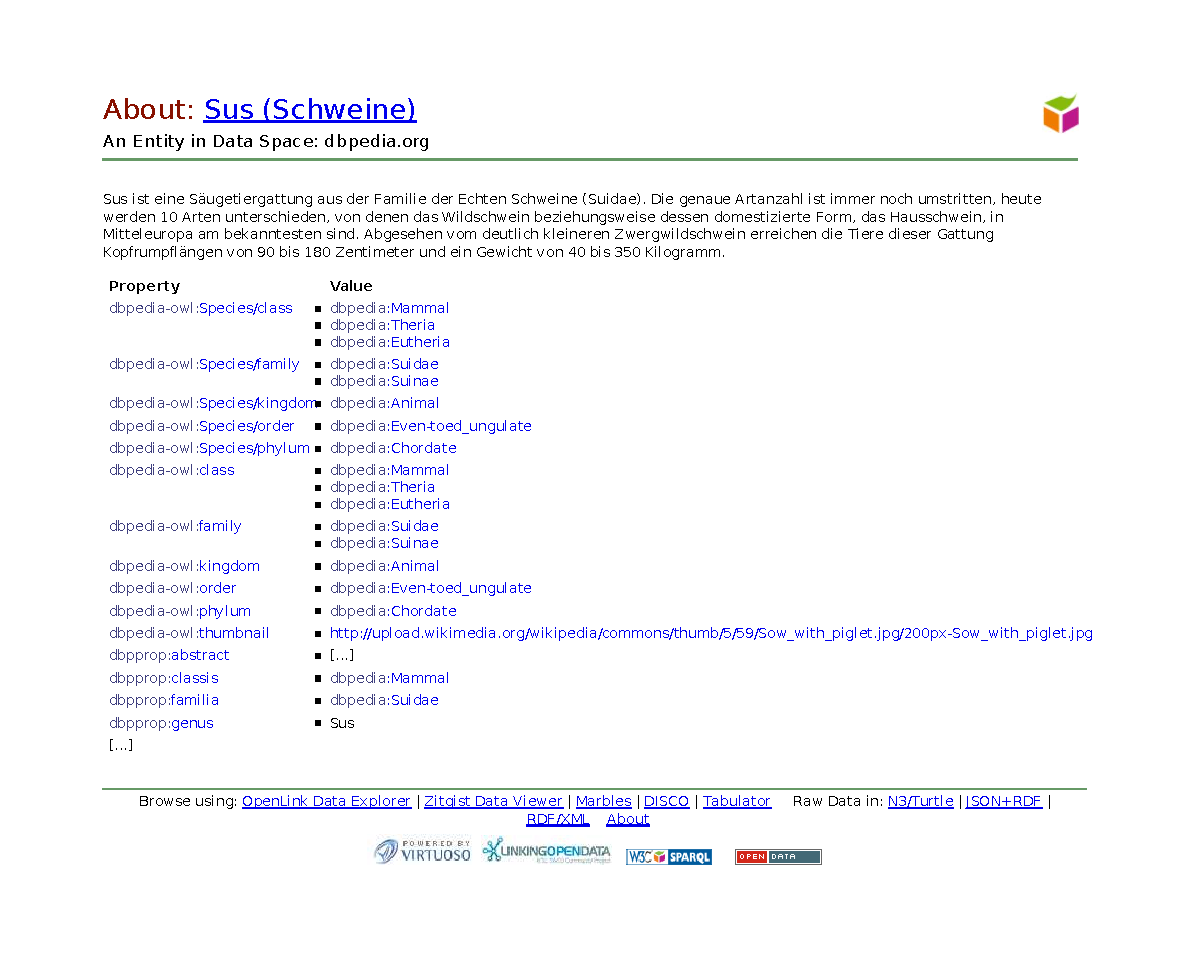
\includegraphics[width=1\textwidth]{img/pdf/pig_anfang.pdf}
\caption[]{Die HTML-Sicht auf den DBpedia-Artikel \url{http://dbpedia.org/resource/pig} (gekürzt, abgerufen am 15.03.2010)}
\label{fig:dbpedia-pig}
\end{figure}

Analog zu \ref{tab:aehnlichkeitsmass-abstracts}:
%Seien $a_1$ und $a_2$ die zu vergleichenden Artikel. 
Seien $P_1$ und $P_2$ die Mengen der enthaltenen Properties sowie v$_1(w)$ und v$_2(w)$ die Anzahl der Vorkommen von $p$ in den beiden DBpedia-Artikeln und f$(p)$ die "`Frequenzklasse"'\footnotemark{} von $p$.
\footnotetext{Analog zur Frequenzklasse von Wörtern: Sei $\f'(p)$ die Frequenz einer Property (die Anzahl der Ressourcen der DBpedia, die mindestens eine Property vom Typ $p$ haben)  und $\f'_{\max}$ die Frequenz der häufigsten Property.
Dann gilt für die Frequenzklasse f der Property:
$f(p)=_{\textnormal{def}}\func{log}_2 \frac{\f'_{\max}}{\f'(p)}$. Bei der Berechnung der Frequenzklasse der Properties wurde auf das Runden verzichtet (im Gegensatz zu der Frequenzklasse der Wörter), es handelt sich also um Fließkommazahlen.}
Da, wie an den Abbildungen \ref{fig:powerlaw_properties_logarithmic_scale} und \ref{fig:zipf_wortschatz_properties} erkennbar ist, auch die Properties $p$ der Entitäten Zipfs Gesetz folgen,
lassen sich auch diese in Frequenzklassen $\f(p)$ einteilen und es ist möglich, eine der im vorigen Kapitel gewählten Gewichtung Ähnliche anzuwenden.
Dann ergibt sich:
%Weiterhin $s_{\max}$ die maximale mögliche Anzahl an Übereinstimmungen der beiden Abstracts sowie $\s_\textnormal{abs}$
%Sei nun s die Funktion s$_{\max}$\\
\begin{subequations}
\begin{align}
\s&_{\textnormal{abs}} 	&:=& \sum_{p\in P_1\cap P_2} \f(p)\cdot\sqrt{\func{v}_1(p)\cdot	\func{v}_2(p)}\\
\s&_{\max}		&:=& \sum_{p\in P_1\cup P_2} \f(p)\cdot\frac{\func{v}_1(p)+	\func{v}_2(p)}{2}\\
\s_{p_1}	&		&:=& \frac{\s_{\textnormal{abs}}}{\s_{\max}}
\end{align}
\label{tab:aehnlichkeitsmass-semantisch}
\end{subequations}

% \subsubsection{Verteilung der Properties}\label{sec:verteilung}
% Um die Gewichtung einer Property, also ihren angenommenen Informationsgehalt, für das semantische Ähnlichkeitsmaß festzulegen, wurde die Verteilung der Properties anhand ihrer Vorkommenshäufigkeit betrachtet.
% Dabei wurde eine Verteilung gemäß eines \emph{power laws}, also eines Potenzgesetzes festgestellt.
% \paragraph{Potenzgesetze}
% Potenzgesetze (engl. \emph{power laws}) beschreiben in der Statistik eine bestimmte Art mathematischer Beziehung zweier Größen und haben die Form
% $f(x) = y = a \cdot x^k+o(x^k)$. Dabei sind $a$ und $k$ Konstanten und $o(x^k)$ ist gegenüber $x^k$ asymptotisch vernachlässigbar.
% Die Funktion f ist \emph{skaleninvariant} mit Skalierungsexponent $k$, das heißt $f(x) \propto f(c\cdot x)$ für jedes $c \in \setR$.
% Aufgrund der teilweise sehr extremen Verteilungen ist es oft schwer, eine solche Beziehung als einem Potenzgesetz entsprechend einzustufen (siehe Abbildung \ref{fig:powerlaw_properties_linear_scale}).
% \begin{figure}[tbh]
% 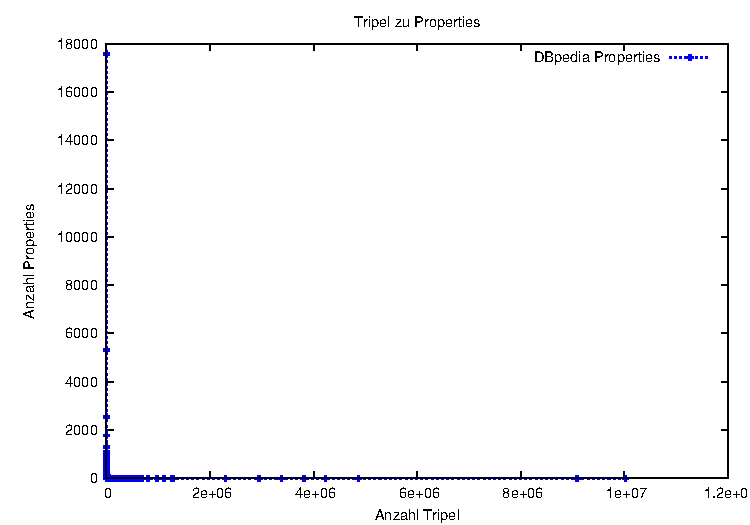
\includegraphics[width=\textwidth]{img/pdf/powerlaw_properties_linscale.pdf}
% \caption[]{Verteilung der Properties der DBpedia bezüglich ihrer Nutzungshäufigkeit (linearer Maßstab)}
% \label{fig:powerlaw_properties_linear_scale}
% \end{figure}
% Aus $y = a \cdot x^k$ folgt $\log(y)= \log(a) + k \cdot \log(x)$.
% Auf einer Darstellung mit logarithmischen Achsen lässt sich also ein linearer Zusammenhang erkennen, falls eine Verteilung gemäß einem Potenzgesetz besteht (siehe Abbildung \ref{fig:powerlaw_properties_logarithmic_scale}).
\begin{figure}[tbh]
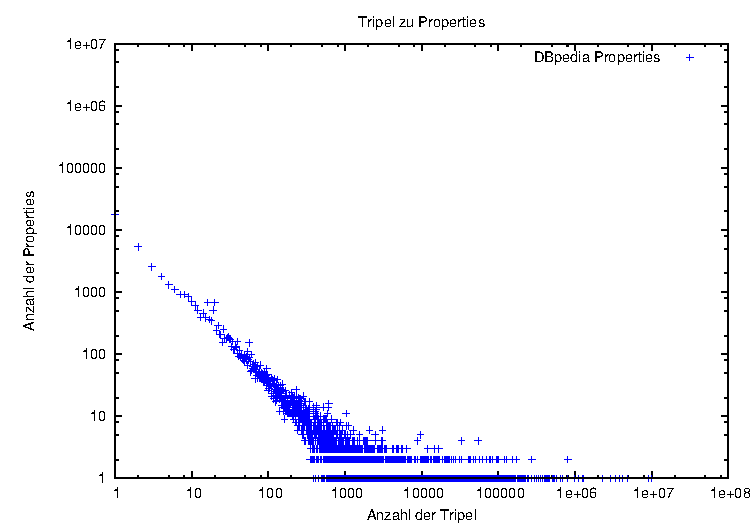
\includegraphics[width=\textwidth]{img/pdf/powerlaw_properties.pdf}
\caption[]{Verteilung der Properties der DBpedia bezüglich ihrer Nutzungshäufigkeit (logarithmischer Maßstab)}
\label{fig:powerlaw_properties_logarithmic_scale}
\end{figure}
%Sehr viele natürliche Phänomene lassen sich mit Potenzgesetzen beschreiben, \zb{} die Größe von Städten, 
% \begin{figure}[tbh]
% 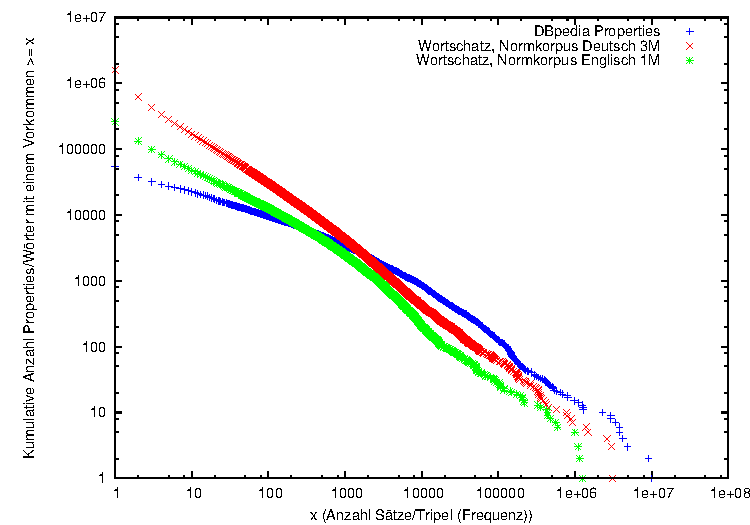
\includegraphics[width=\textwidth]{img/pdf/pareto_wortschatz_properties.pdf}
% %\caption{}
% \label{fig:pareto_wortschatz_properties}
% \end{figure}

\begin{figure}[tbh]
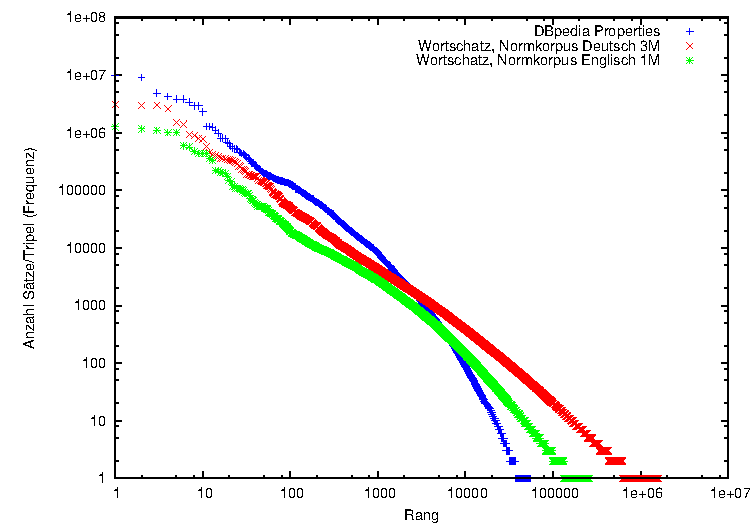
\includegraphics[width=\textwidth]{img/pdf/zipf_wortschatz_properties_reduced.pdf}
%\caption{}
\label{fig:zipf_wortschatz_properties}
\end{figure}

% \begin{figure}[tbh]
% 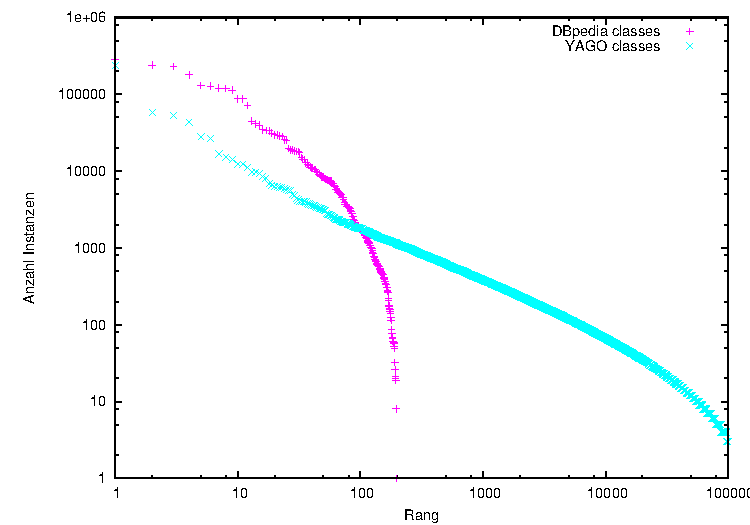
\includegraphics[width=\textwidth]{img/pdf/zipf_hierarchy_reduced.pdf}
% %\caption{}
% \label{fig:zipf_hierarchy}
% \end{figure}

%Außerdem wird die Nähe der zu vergleichenden Klassen in verschiedenen Hierarchien als Hinweis auf eine Ähnlichkeit gewertet.

%umgedreht könnte man auch machen wird aber nicht gemacht

Ein wichtiger Unterschied zwischen den Abstracts der Wikipedia-Artikel und der aus diesen Artikeln extrahierten DBpedia-Daten ist jedoch, dass
die Einleitungen alle ungefähr die gleiche Länge haben und von Menschen mit dem Zweck geschrieben wurden, alle relevanten Informationen zu diesem Thema aufzuführen.
Aus diesem Grund kann das Vorkommen eines Wortes in dem einen Abstract und das Fehlen desselben im Anderen als Indiz dafür aufgefasst werden, dass das eine Konzept ein bestimmtes Merkmal aufweist,
das Andere jedoch nicht. Weiterhin kann die Anzahl der Vorkommen des Wortes Hinweise auf auf die Stärke der Ausprägung des Merkmals geben.
Da die Länge der Wikipedia-Artikel jedoch stark variiert und die Properties nur aus einem Teil der Artikel gewonnen werden (vor allem aus den Infoboxen), ist es fraglich, ob die Anzahl des Vorkommens
einer bestimmten Property in den Ähnlichkeitswert einfließen sollte oder ob die wichtigste Information ist, dass beide Konzepte überhaupt diese Property aufweisen.

\begin{bsp}
Wir vergleichen die Artikel \article{Gordon_Bethune} und \article{Sam_Walton}.
Beide weisen die Property \property{dbpedia-owl:occupation} auf.\\
~\\
\article{Gordon_Bethune} \property{dbpedia-owl:occupation}
\begin{itemize}
\item \article{dbpedia:Continental_Airlines}
\item \article{dbpedia:Braniff}
\item \article{dbpedia:Boeing}
\item \article{dbpedia:Piedmont_Airlines}
\end{itemize}
\article{Sam_Walton} \property{dbpedia-owl:occupation}
\begin{itemize}
\item \article{dbpedia:Wal-Mart}
\item \article{dbpedia:Chairman}
\end{itemize}
\end{bsp}

Die wichtige Information hierbei ist, dass beide Entitäten eine Arbeit besitzen oder besaßen, also Arbeiter sind oder waren.
Dass die eine Person dabei bereits vier Stellen besaß und die andere Zwei (tatsächlich wohl nur eine, da \emph{Chairman} sicherlich eine Position ist und kein Arbeitgeber), ist in diesem Fall kein wesentliches Merkmal.
Aufgrund der \emph{Open World Assumption} kann es ja weitere Angestelltenbeziehungen geben, die nur nicht in der DBpedia enthalten sind.
Aus diesem Grund wurde die Vorkommenshäufigkeit v$(p)$ aus Formel \ref{tab:aehnlichkeitsmass-semantisch} entfernt.
%Es ist also fraglich, ob die Vorkommenshäufigkeit v$(p)$ in Formel \ref{aehnlichkeitsmass-semantisch} zu integrieren ist oder nicht.
%Da es jedoch unklar ist, inwieweit dieses Beispiel zu verallgemeinern ist, wurden beide Möglichkeiten implementiert und in die Evaluierung der Disambiguierung einbezogen.
Natürlich ist nicht nur das gemeinsame Vorhandensein einer Property (\emph{schwache Beziehung} in Tabelle \ref{tab:beispiel-aehnlichkeitsmass}) eine wichtige Information sondern auch, worauf sie verweist.
Sind die Objekte bei beiden Artikeln dieselben (\emph{indirekte Beziehung} in Tabelle \ref{tab:beispiel-aehnlichkeitsmass}), ist dies natürlich ein stärkerer Indikator für eine Übereinstimmung.
%Ist dies nicht der Fall, kann die Ähnlichkeit dieser Objekte noch rekursiv mittels t oder auch mittels eines taxonomischen Vergleiches berechnet werden, dies wurde jedoch aus Laufzeitgründen nicht durchgeführt.
Aus diesen Überlegungen ergibt sich:

\begin{subequations}%\label{aehnlichkeitsmass-semantisch}
\begin{align}
\func{s}&_{\textnormal{abs}} 	&:=& \sum_{p\in P_1\cap P_2} \f(p)\cdot \alpha \\
\func{s}&_{\max}		&:=& \sum_{p\in P_1\cup P_2} \f(p)
\end{align}
\end{subequations}

Mit
$\alpha = 
\begin{cases}
1 &\exists o: (a_1,p,o) \land (a_2,p,o)\footnotemark{}\\%\textnormal{{falls beide Artikel ein Vorkommen von $p$ mit demselben Objekt o haben}\\
c &\textnormal{sonst}, 0 < c < 1
\end{cases}$
\footnotetext{Informell: Falls beide Artikel ein Vorkommen der Property $p$ mit demselben Objekt $o$ haben.}

Daraus ergeben sich jedoch Schwierigkeiten:
Ist $c$ zu klein, dann wird die Bedeutung des Vorhandenseins gleicher Properties unterschätzt, ist $c$ zu groß, dann wird sie überschätzt und das alleinige Vorhandensein einer seltenen Property 
kann schwerer wiegen als die Übereinstimmung in einer häufigen Property inklusive desselben Objektes. Sehr häufige Properties wie \property{rdf:type} oder \property{skos:subject} fallen sogar ganz weg,
da sie eine Frequenzklasse von 0 besitzen. Außerdem sind durch die Multiplikation mit $c$ die resultierenden Ähnlichkeitswerte sehr klein.
Dieses Problem wird behoben, indem die Frequenzklasse nicht einbezogen wird, falls Objektgleichheit vorliegt:

\begin{equation}
\s_{\textnormal{abs}} := \sum_{p\in P_1\cap P_2}
\begin{cases}
d &\exists o: (a_1,p,o) \land (a_2,p,o), d > 1\\
\f(p) &\textnormal{sonst}\\%\textnormal{{falls beide Artikel ein Vorkommen von $p$ mit demselben Objekt o haben}\\
\end{cases}
\end{equation}

Um die Normierung zu gewährleisten folgt daraus:
\begin{equation}
\s_{\max} := \sum_{p\in P_1\cup P_2} \max(\f(p),d)\\
\end{equation}

\begin{rem}\label{rem:properties-exclusion-1}
Einige der häufigsten Properties werden nicht in die Berechnung einbezogen.
\begin{figure}[H]
\property{rdf:type}\\
\property{skos:subject}
%\end{quote}
\caption{Properties, die Klassenzugehörigkeiten anzeigen}
\label{fig:properties_exclusion_1}
\end{figure}
Diese Properties werden separat über Hierarchien behandelt, siehe Abschnitt \ref{sec:hierarchien}.
Weitere Properties wurden ausgeschlossen, weil sie Artikeldetails beschreiben, die keine Hinweise auf die Ähnlichkeit der beschriebenen Gegenstände liefern, siehe Abbildung \ref{fig:properties_exclusion_2}.
\begin{figure}[H]
%\begin{quote}
\property{dbpprop:wikiPageUsesTemplate}\\
\property{dbpprop:imageWidth}\\
\property{foaf:depiction}\\
\property{foaf:name}\\
\property{foaf:page}\\
\property{dbpprop:imageCaption}\\
%\end{quote}
\caption{ausgeschlossene Properties}
\label{fig:properties_exclusion_2}
\end{figure}
\end{rem}

Bei einer ersten Auswertung des Ähnlichkeitsmaßes $s_p$ angewandt auf die Testdaten aus Abschnitt \ref{sec:aehnlichkeitsmass-abstract} (siehe Tabelle \ref{tab:aehnlichkeitsmass-semantisch-properties-1})
ergibt sich ein sehr hoher Wert für das Paar (\article{Wild_boar}, \article{Pig}).
Nimmt man die gleiche Einteilung vor wie bei Tabelle \ref{tab:einschaetzung}, dann ergibt sich folgende Reihenfolge:
\begin{center}
\begin{tabular}{lllllll}
1	&$>$	&$3,9$	&$>$	&$6, 10, 2, 8$	&$>$ &$5,7,4$\\
\end{tabular}
\end{center}
Dieses Ergebnis stimmt nicht mit der manuellen Einschätzung aus Tabelle \ref{tab:einschaetzung} überein.
Weiterhin fällt auf, dass in Tabelle \ref{tab:aehnlichkeitsmass-semantisch-properties-1} mehrere Artikelpaare den gleichen Ähnlichkeitswert aufweisen.
Um die Ursache für diese Probleme zu untersuchen, werden die gemeinsamen Properties der getesteten Artikel betrachtet (siehe Tabelle \ref{tab:properties-intersection}).
Unter diesen befinden sich immer noch einige Properties, die Details des Artikels und nicht des Artikelgegenstandes beschreiben.
Abbildung \ref{tab:properties_exclusion_3} zeigt weitere Properties, die daher zusätzlich zu denen aus Abbildung \ref{fig:properties_exclusion_2} entfernt wurden.
\begin{figure}[H]
%\begin{quote}
\property{dbpedia-owl:thumbnail}\\
\property{dbpprop:relatedInstance}\\
\property{dbpprop:wikiPageUsesTemplate}\\
\property{dbpedia-owl:thumbnail}\\
\property{dbpprop:hasPhotoCollection}\\
\property{dbpprop:name}\\
%\end{quote}
\caption{weitere ausgeschlossene Properties}
\label{tab:properties_exclusion_3}
\end{figure}

Eine Anwendung der Ähnlichkeitsmaßes $\s_p$ auf die Testdaten, bei denen auch die Properties aus Tabelle \label{tab:properties_exclusion_3} ignoriert werden, erhöht den Ähnlichkeitswert des Paares (\article{Wild_boar}, \article{Pig}) auf \val{0.9568}, resultiert jedoch
in einem Ähnlichkeitswert von 0 für alle weiteren Paare (siehe Tabelle \ref{tab:aehnlichkeitsmass-semantisch-properties-2}).

Dies liegt daran, dass für alle hier getesteten DBpedia-Artikel bis auf \article{Wild_boar} und \article{Pig} keine ausführlichen Daten vorliegen.
Die Daten der DBpedia werden per automatischer Extraktion aus Wikipedia-Infoboxen erzeugt.
Dadurch kann beispielsweise zwischen den Artikeln \article{Wild_boar} und \article{Elephant} keine Ähnlichkeit festgestellt werden (siehe Abbildungen \ref{fig:wikipedia-wild_boar} und \ref{fig:wikipedia-elephant}).

%foaf:depiction, relatedInstance	&thumbnail, wikiPageUsesTemplate, piction, hasPhotoCollection	&	&~\\
%\midrule
%Starship\_Enterprise	&wikiPageUsesTemplate, name, relatedInstance	&wikiPageUsesTemplate, name, hasPhotoCollection	&wikiPageUsesTemplate, hasPhotoCollection, relatedInstance
%\item [1] Differenzen von weniger als 0,01 wurden als $\approx$ gewertet.

\begin{center}
\begin{table}
\begin{threeparttable}
\begin{tabular}{llll}
\toprule
Artikel 1 		&Artikel 2 		&Ähnlichkeitswert	&$\delta$\tnote{1}\\
\midrule
Wild\_boar		&Pig		&\val{0.8679}		&\val{0.7112}\\
Wild\_boar		&Elephant		&\val{0.1567}		&\val{0.0000}\\
Wild\_boar		&Outer\_space		&\val{0.1567}		&\val{0.0163}\\
Wild\_boar		&Starship\_Enterprise		&\val{0.1404}		&\val{0.0095}\\
Elephant		&Outer\_space		&\val{0.1309}		&\val{0.0048}\\
Pig			&Elephant		&\val{0.1261}		&\val{0.0000}\\
Pig			&Outer\_space		&\val{0.1261}		&\val{0.0163}\\
Pig			&Starship\_Enterprise		&\val{0.1098}		&\val{0.0000}\\
Elephant		&Starship\_Enterprise		&\val{0.1098}		&\val{0.0000}\\
Starship\_Enterprise	&Outer\_space		&\val{0.1098}		&\\
\midrule
$\average$		&			&	0.2034&\\
\bottomrule
\end{tabular}
\begin{tablenotes}
\item [1] In Zeile i: Die Differenz des Ähnlichkeitswertes zwischen Zeile i und Zeile i+1
\end{tablenotes}
\caption{Werte von $s_p$ unter Ausschluß der Properties aus den Abbildungen \ref{fig:properties_exclusion_1} und \ref{fig:properties_exclusion_2}.}
\label{tab:aehnlichkeitsmass-semantisch-properties-1}
\end{threeparttable}
\end{table}
\end{center}

\begin{center}
\begin{table}
\begin{threeparttable}
\begin{tabular}{llll}
\toprule
Artikel 1 		&Artikel 2 		&Ähnlichkeitswert	&$\delta$\tnote{1}\\
\midrule
Wild\_boar		&Pig		&\val{0.9568}		&\val{0.9568}\\
Wild\_boar		&Elephant		&\val{0.0000}		&\val{0.0000}\\
Wild\_boar		&Starship\_Enterprise		&\val{0.0000}		&\val{0.0000}\\
Wild\_boar		&Outer\_space		&\val{0.0000}		&\val{0.0000}\\
Pig		&Elephant		&\val{0.0000}		&\val{0.0000}\\
Pig		&Starship\_Enterprise		&\val{0.0000}		&\val{0.0000}\\
Pig		&Outer\_space		&\val{0.0000}		&\val{0.0000}\\
Elephant		&Starship\_Enterprise		&\val{0.0000}		&\val{0.0000}\\
Elephant		&Outer\_space		&\val{0.0000}		&\val{0.0000}\\
Starship\_Enterprise	&Outer\_space		&\val{0.0000}		&\\
\midrule
$\average$		&			&0.0957		&\\
\bottomrule
\end{tabular}
\begin{tablenotes}
\item [1] In Zeile i: Die Differenz des Ähnlichkeitswertes zwischen Zeile i und Zeile i+1
\end{tablenotes}
\caption{Werte von $s_p$ unter Ausschluß der Properties aus den Abbildungen \ref{fig:properties_exclusion_1}, \ref{fig:properties_exclusion_2} und \ref{fig:properties_exclusion_3}.}
\label{tab:aehnlichkeitsmass-semantisch-properties-2}
\end{threeparttable}
\end{table}
\end{center}


\begin{sidewaystable}
\footnotesize
\begin{tabular}{lp{4cm}p{4cm}p{4cm}p{4cm}}
\toprule
~	&Wild\_boar	&Pig	&Elephant	&Starship\_Enterprise\\
\midrule
Pig	&Species/class, Species/family, Species/kingdom, Species/order, Species/phylum, dbpedia-owl:class, dbpedia-owl:family, dbpedia-owl:kingdom, dbpedia-owl:order, dbpedia-owl:phylum, thumbnail, dbpprop:classis, dbpprop:familia, dbpprop:genus, dbpprop:name, dbpprop:ordo, dbpprop:phylum, dbpprop:regnum, , foaf:name	&	&	&\\
\midrule
Elephant	&thumbnail, relatedInstance, 	&thumbnail, hasPhotoCollection	&	&\\
\midrule
Starship\_Enterprise	&dbpprop:name, relatedInstance, 	&hasPhotoCollection, dbpprop:name, 	&hasPhotoCollection, relatedInstance, 	&\\
\midrule
Outer\_space	&thumbnail, relatedInstance	&thumbnail, hasPhotoCollection	&thumbnail, hasPhotoCollection, relatedInstance	&hasPhotoCollection, relatedInstance\\
\bottomrule
\end{tabular}
\caption[]{
Gemeinsame Properties der Artikel \article{Wild_boar}, \article{Pig}, \article{Elephant}, \article{Starship_Enterprise}. Ohne die in Bemerkung \ref{rem:properties-exclusion-1} aufgeführten Properties.\\
Aus Platzgründen sind einige Präfixe nicht aufgeführt.
}
\label{tab:properties-intersection}
\end{sidewaystable}

\begin{figure}[tbh]
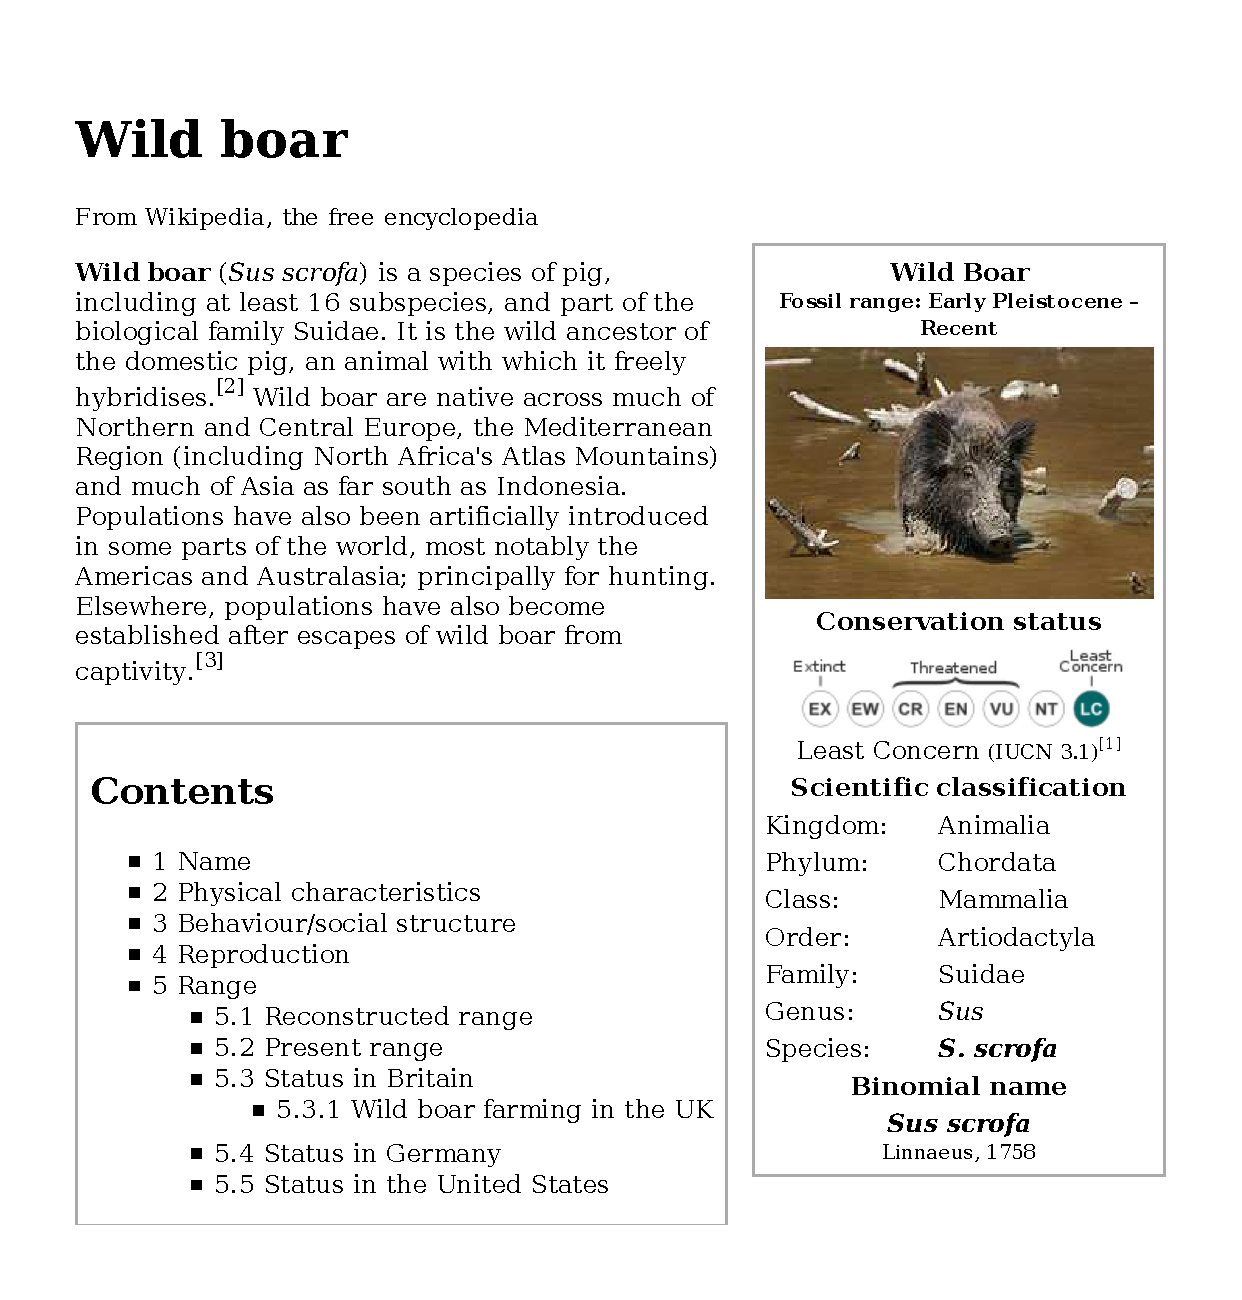
\includegraphics[width=0.99\textwidth]{img/pdf/wild_boar_wikipedia.pdf}
\caption[]{Der Wikipedia-Artikel \url{http://en.wikipedia.org/wiki/Wild_boar} (teilweise abgebildet, aufgerufen am 17.03.2010) enthält eine automatisch verarbeitbare \emph{Infobox}.}
\label{fig:wikipedia-wild_boar}
\end{figure}

\begin{figure}[tbh]
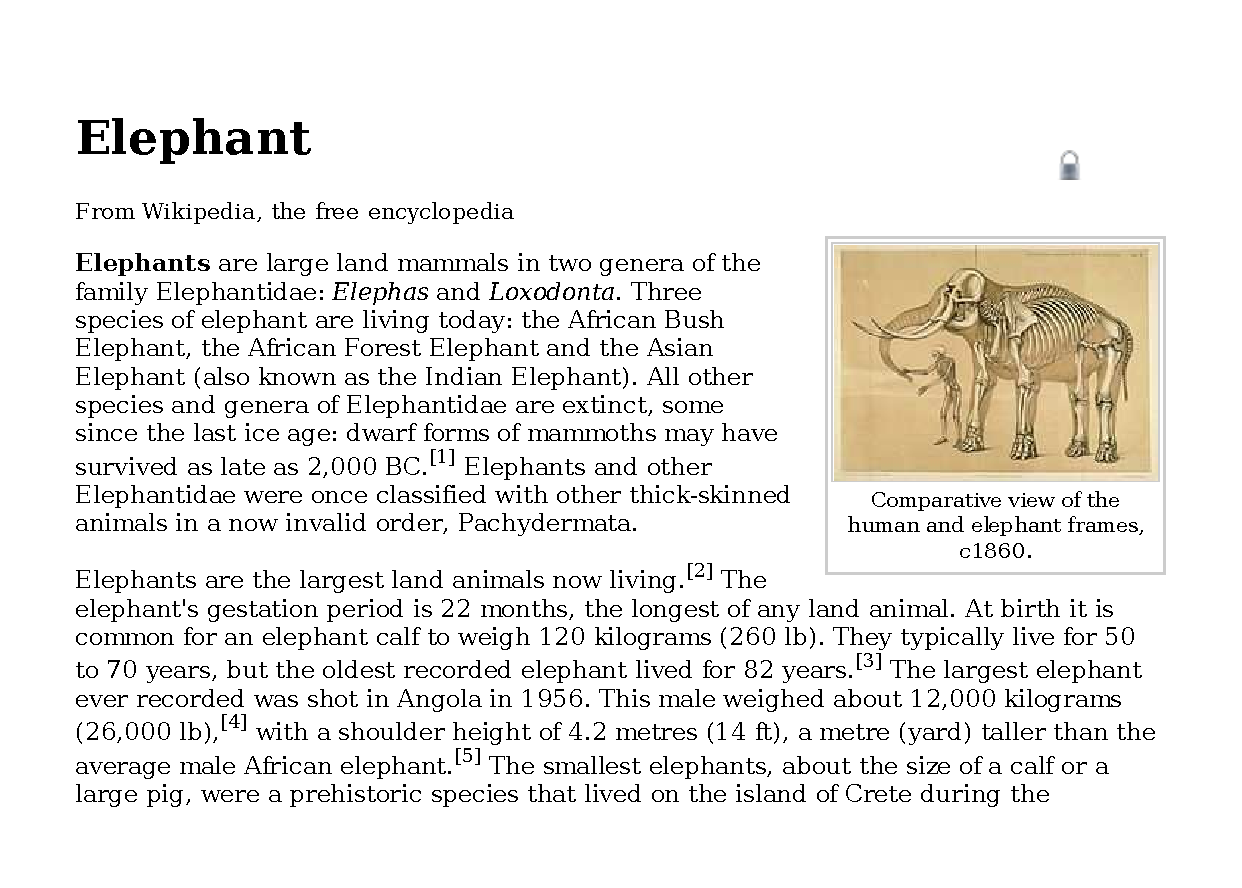
\includegraphics[width=0.99\textwidth]{img/pdf/elephant_wikipedia.pdf}
\caption[]{Der Wikipedia-Artikel \url{http://en.wikipedia.org/wiki/Elephant} (teilweise abgebildet, aufgerufen am 17.03.2010) enthält keine Infobox.}
\label{fig:wikipedia-elephant}
\end{figure}

\subsubsection{Version 2}
Bei näherer Betrachtung von Version 1 des Ähnlichkeitsmaßes der Properties fallen einige Schwächen auf.
So werden Ähnlichkeiten nur dann festgestellt, wenn beide Entitäten dieselbe Property aufweisen und vorzugsweise noch dasselbe Objekt haben.
Es existieren jedoch noch einige weitere Verbindungen, die auf eine Ähnlichkeit oder eine Beziehung zwischen zwei Entitäten schließen lassen.
Aus diesem Grund wurde eine zweite Version des Ähnlichkeitsmaßes entworfen, die eine größere Anzahl an Beziehungstypen in Betracht zieht.
Seien $aRx$ und $bRx$ (bzw. $(a,p,x)$ und $(b,p,x)$) zwei Tripel, wobei $a$ und $b$ als Subject, $R$ bzw. $p$ als property und $x$ als Objekt fungieren.
\begin{table}[h]
\begin{center}
\begin{tabular}{llll}
\toprule
	&Beziehung			&			&Hinweis auf\\
\midrule
a	&direkt				&$aRb \lor  bRa$	&Ähnlichkeit, Beziehungsstärke\\
b	&stark indirekt 		&$aRx \land bRx$	&Ähnlichkeit, Beziehungsstärke\\
c	&schwach indirekt		&$aRx \land bSy$	&Beziehungsstärke\\
d	&gleiche Property		&$aRx \land bRy$	&Ähnlichkeit, Beziehungsstärke\\
\bottomrule
\end{tabular}
\end{center}
\caption{Beziehungstypen zwischen zwei Entitäten $a$ und $b$ in Reihenfolge ihrer Beziehungsstärke}
\label{tab:disambiguierung-properties}
\end{table}

\begin{figure}[H]
\centering
\subfloat[]{
\Tree[2]{
\K{a}\B{d}^{R}\\
\K{b}\\
} 
}
\subfloat[]{
\Tree[-1]
{
		&\K{x}\B{dl}_{R}\B{dr}^{R}\\
\K{a}		&			&\K{b}\\
} 
}
\subfloat[]{
\Tree[-1]
{
		&\K{x}\B{dl}_{R}\B{dr}^{S}\\
\K{a}		&			&\K{b}\\
} 
}
\subfloat[]{
\Tree[-1]
{
\K{a}\B{d}^{R}	&\K{b}\B{d}^{R}\\
\K{x}		&\K{y}\\
} 
}
\end{figure}

Sei $T$ die Menge aller in der DBpedia enthaltenen Tripel und seien $T_a$ und $T_b$ die Mengen der Tripel mit $a$ und $b$ als Subjekt, $T_a = \{t=(s,p,o)\in T| s = a\}$,
$T_b = \{t=(s,p,o)\in T| s = b\}$.
%Seien weiterhin $P_a$ und $P_b$ die Menge aller Properties aus $T_a$ und $T_b$, $P_a = \{p|\exists o: (a,p,o) \in T_a\}$, $P_b = \{p|\exists o: (b,p,o) \in T_b\}$.
Aus Tabelle \ref{tab:disambiguierung-properties} lässt sich nun folgendes Ähnlichkeitsmaß konstruieren:

\begin{align}
\s_{p_2}(a,b)	&= \frac{\sum_{t \in T_a} \s_{p_1}(t,b,T_b)+\sum_{t \in T_b} \s_{p_2}'(t,a,T_a)}{|T_a|+|T_b|}
\end{align}
mit
\begin{equation}
\s_{p_2}'((s,p,o),x,T') = 
\begin{cases}
1 					&\text{wenn } o=x\\
1 					&\text{wenn } \exists (x,p,o) \in T'\\
\alpha<1				&\text{wenn } \exists p': 	\exists (x,p',o) \in T'\\
1-\frac{1}{\val{0.1}\cdot f(p)+1}	&\text{wenn } \exists o':	\exists (x,p,o') \in T'\\
\end{cases} 
\end{equation}
%f(p) die Frequenzklasse der Property ist.
Die einzelnen Fälle lassen sich dabei wie folgt begründen:

\begin{align*}
1 			&\text{  wenn } o=x
\end{align*}
In diesem Fall gilt entweder $t = (a,p,b)$ oder $(b,p,a)$, was eine direkte Beziehung und damit ein starkes Indiz für eine Ähnlichkeit ist.

\begin{align*}
1 			&\text{  wenn } \exists (x,p,o) \in T'\\
\end{align*}
In diesem Fall gibt es eine stark indirekte Beziehung, was auch ein starkes Indiz für eine Ähnlichkeit ist.

\begin{align*}
\alpha<1		&\text{  wenn } \exists p': 	\exists (x,p',o) \in T'\\
\end{align*}
Es existiert eine schwach indirekte Beziehung, was ein etwas schwächeres Indiz für eine Ähnlichkeit ist. Alpha wurde dabei auf $\alpha = 0,7$ festgelegt.

\begin{align*}
1-\frac{1}{0,1 \cdot f(p)+1}	&\text{  wenn } \exists o':	\exists (x,p,o') \in T'\\
\end{align*}

Beide Entitäten haben nur das Vorhandensein der gleichen Property gemein, jedoch mit verschiedenen Objekten. Die Stärke der draus gewonnenen Information ist hierbei davon abhängig, wie häufig die Property $p$ ist.
\article{dbpedia-owl:location} beispielsweise hat ohne gleiches Objekt fast gar keine Aussagekraft, \article{dbpedia-owl:vicePresident} hingegen schon, da es die Aussage erlaubt, dass das Konzept eine Person beschreibt, 
die ein Präsident von etwas ist, was eine starke Einschränkung der Gesamtmenge aller Konzepte ist.
In diesem Fall erfolgt keine Gewichtung verschiedener Terme sondern es ist ein einzelner Ähnlichkeitsteilwert für ein Tripel gesucht. Dieser Wert wurde zunächst durch $1-\frac{1}{f(p)+1}$ (Abbildung \ref{fig:1minus1durch1plusx}) berechnet,
dann jedoch auf $1-\frac{1}{0,1 \cdot f(p)+1}$ (Abbildung \ref{fig:1minus1durch1plusxdurch10}) abgeändert,
um erst ab einer Frequenzklasse von 10 (was einer Property entspricht, die $\approx$ 1000 mal so selten ist wie die Häufigste) einen Wert von 0,5 zu erhalten.

\begin{figure}[H]
\subfloat[$1-\frac{1}{f(p)+1}$]{
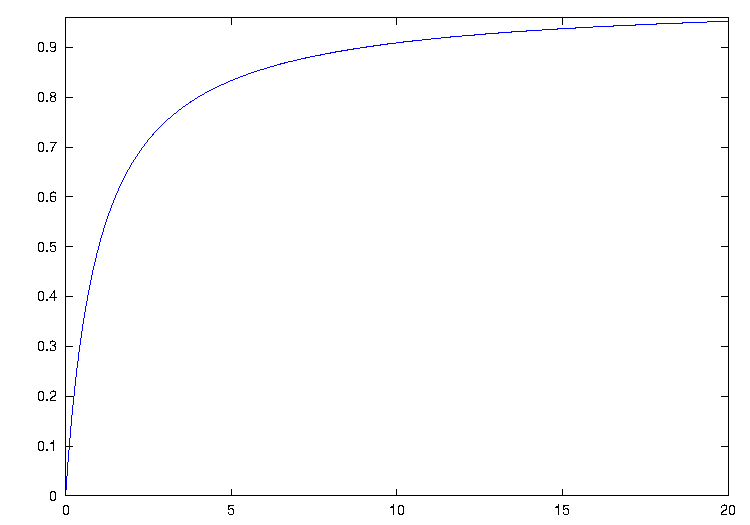
\includegraphics[width=0.5\textwidth]{img/pdf/1minus1durch1plusx.pdf}
\label{fig:1minus1durch1plusx}
}
\subfloat[$1-\frac{1}{0,1 \cdot f(p)+1}$]{
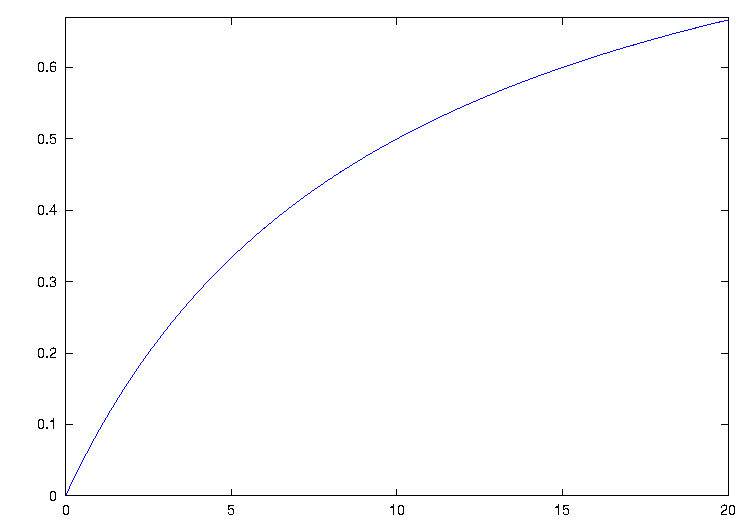
\includegraphics[width=0.5\textwidth]{img/pdf/1minus1durch1plusxdurch10.pdf}
\label{fig:1minus1durch1plusxdurch10}
}
\caption{verschiedene Gewichtungen der Frequenzklasse einer Property}
\end{figure}


\subsubsection{Anwendung}
Die Property-basierten Ähnlichkeitsmaße eignen sich gut für Entitäten, die zwar nicht besonders ähnlich sind aber auf gemeinsame Elemente verweisen oder die in den Hierarchien auf der gleichen Stufe stehen.
Die Tabellen \ref{tab:aehnlichkeitsmass-semantisch-properties-version1} und \ref{tab:aehnlichkeitsmass-semantisch-properties-version2} zeigen, dass den Städten aus dem gleichen Land höhere Werte zugewiesen werden.
Da $s_{p_2}$ hier unähnlichere Paare stärker abstraft, wird im Folgenden nur noch $s_{p_2}$ verwendet.

\begin{table}
\begin{tabular}{lll}
\toprule
Konzeptpaar					&Ähnlichkeitswert $\s_{p}$\\
\midrule
Leipzig		&Dresden		&0,5381\\
Borna		&Leipzig		&0,5359\\
London		&Liverpool		&0,4677\\
Borna		&Dresden		&0,4633\\
Dresden		&London		&0,4037\\
Dresden		&Liverpool		&0,4037\\
Leipzig		&London		&0,3359\\
Leipzig		&Liverpool		&0,3359\\
Borna		&London		&0,3322\\
Borna		&Liverpool		&0,3322\\
\bottomrule
\end{tabular}
\caption{Werte der Ähnlichkeitsfunktion $\s_{p}$ von einigen Städten}
\label{tab:aehnlichkeitsmass-semantisch-properties-version1}
\end{table}


\begin{table}
\begin{tabular}{lll}
\toprule
Konzeptpaar					&Ähnlichkeitswert $\s_{p_2}$\\
\midrule
Borna		&Leipzig		&0,4816\\
Leipzig		&Dresden		&0,4094\\
Borna		&Dresden		&0,3863\\
London		&Liverpool		&0,3535\\
Dresden		&London		&0,1652\\
Dresden		&Liverpool		&0,1381\\
Borna		&Liverpool		&0,1185\\
Leipzig		&Liverpool		&0,1062\\
Borna		&London		&0,1021\\
Leipzig		&London		&0,0918\\
\bottomrule
\end{tabular}
\caption{Werte der Ähnlichkeitsfunktion $\s_{p_2}$ von einigen Städten}
\label{tab:aehnlichkeitsmass-semantisch-properties-version2}
\end{table}

\FloatBarrier
\subsection{Ähnlichkeit durch Hierarchien}\label{sec:hierarchien}

Es werden folgende Hierarchien benutzt (näher beschrieben in Abschnitt \ref{sec:grundlagen-hierarchien}):
\begin{itemize}
 \item Wikipediakategorien
 \item YAGO
 \item DBpedia-Klassen
\end{itemize}
\iffalse
@article{DBLP:journals/computer/Brachman83,
  author    = {Ronald J. Brachman},
  title     = {What IS-A Is and Isn't: An Analysis of Taxonomic Links in
               Semantic Networks},
  journal   = {IEEE Computer},
  volume    = {16},
  number    = {10},
  year      = {1983},
  pages     = {30-36},
  bibsource = {DBLP, http://dblp.uni-trier.de}
}

SELECT ?o WHERE
{
<http://dbpedia.org/resource/Ant> a ?o.
}

owl:Thing [http]
<http://sw.opencyc.org/2008/06/10/concept/Mx4rvVjf5JwpEbGdrcN5Y29ycA> [http]
dbpedia:ontology/Species [http]
dbpedia:ontology/Animal [http]
dbpedia:ontology/Insect [http]
dbpedia:ontology/Eukaryote [http]

SELECT ?o WHERE
{
<http://dbpedia.org/resource/Pig> a ?o.
}

owl:Thing [http]
dbpedia:ontology/Species [http]
dbpedia:ontology/Animal [http]
dbpedia:ontology/Mammal [http]
<http://sw.opencyc.org/2008/06/10/concept/Mx4rvVjLLJwpEbGdrcN5Y29ycA> [http]
dbpedia:ontology/Eukaryote [http]

SELECT ?o WHERE
{
<http://dbpedia.org/resource/Pig> skos:subject ?o.
}

:Category:Even-toed_ungulates [http]
:Category:Pigs [http]

PREFIX owl: <http://www.w3.org/2002/07/owl#>
PREFIX xsd: <http://www.w3.org/2001/XMLSchema#>
PREFIX rdfs: <http://www.w3.org/2000/01/rdf-schema#>
PREFIX rdf: <http://www.w3.org/1999/02/22-rdf-syntax-ns#>
PREFIX foaf: <http://xmlns.com/foaf/0.1/>
PREFIX dc: <http://purl.org/dc/elements/1.1/>
PREFIX : <http://dbpedia.org/resource/>
PREFIX dbpedia2: <http://dbpedia.org/property/>
PREFIX dbpedia: <http://dbpedia.org/>
PREFIX skos: <http://www.w3.org/2004/02/skos/core#>

Problem: skos-categorien sind mit skos:broader verbunden statt mit rdf:type
-> egal, wir benutzen sowieso yago
-> mal gucken wies da aussieht
\fi

%Da ein Baum ein Spezialfall eines DAG ist, wird in diesem Abschnitt zuerst eine Methode zur Ähnlichkeitsbestimmung anhand einer Polyhierarchie vorgestellt.
In diesem Abschnitt wird zuerst eine Methode zur Ähnlichkeitsbestimmung anhand einer Polyhierarchie vorgestellt.
Darauf folgt ein laufzeitoptimiertes Verfahren, welches bei Monohierarchien ein exaktes Ergebnis liefert, bei Polyhierarchien jedoch immer noch eine gute Näherung.

% die blätter von dem baum sind dann die instanzen
% und die direkten superklassen sind die typen
% -> nee das ist blöd, die blätter sind die typen und die artikel bilden nen count oder so
% -> obwohl das unintuitiv ist erstes ist vielleicht doch besser
% - in der hierarchie sind aber nur die klassen drin und nicht die instanzen also das 2.
\paragraph{Aufgabenstellung}
Sei $G$ eine Hierarchie, $G = (V,E)$.
Seien $T_1, T_2 \subseteq V$ die Klassen (Typen) der DBpedia-Entitäten $a_1$ und $a_2$. %, $T_{i} = \func{classes}(a_{i})$.
%Sei weiterhin $E^+$ die \emph{transitive Hülle}\footnotemark{} der Relation $E$, sowie $T^\star$ die Menge aller Superklassen von $T$, $T^\star = \{v \in V| \exists t \in T: t E^+ v\}$.
%\footnotetext{$x \ E^{+} \ y : \Leftrightarrow \exists n \geq 0 \ \exists e_1,\dots ,e_n \in V: x \,E \,e_1 \,E \,e_2 \,E \dots \,E \,e_n \,E \,y$.}
Gesucht ist nun ein Ähnlichkeitsmaß $\s_h: \pow{V} \times \pow{V} \rightarrow [0,1] \subset \setR$.

\paragraph{Erster Lösungsansatz}
\newcommand{\snaiv}{\s_{\h_0}}
Ein naiver Ansatz ist, den Anteil gleicher Klassen der beiden Individuen zu bestimmen:
\begin{equation*}
\snaiv := \frac{|(T_1 \cap T_2)|}{|(T_1 \cup T_2)|} 
\end{equation*}

Diese Methode ermöglicht jedoch nur eine sehr mangelhafte Aussage über die Ähnlichkeit der Entitäten $a_1$ und $a_2$.
Klassen, die nicht übereinstimmen, führen zu einer Abwertung des Ähnlichkeitswertes.
Aufgrund der Offene-Welt-Annahme ist jedoch auch bei den Entitäten, deren Zuordnung zu einer bestimmten Klasse nicht explizit definiert wurde, die Zugehörigkeit zu dieser Klasse möglich.
Weiterhin sorgt diese Methode für sehr hohe Ähnlichkeitswerte bei Paaren, die eine sehr geringe Anzahl an Klassenzuordnungen besitzen, welche sehr nahe an der Wurzel liegen.

\begin{table}
\begin{tabular}{ll}
\toprule
Entität		&Klassen\\
\midrule
London		&owl:Thing, City\\
Pig		&owl:Thing, Animal\\
Elephant	&owl:Thing, Animal\\
Dog		&owl:Thing, Animal, Mammal, Carnivora\\
Human		&owl:Thing, Animal, Mammal, Primate\\
Mensch		&owl:Thing, Animal, Mammal, Primate\\
\bottomrule
\end{tabular} 
\caption{fiktive Klassenzuordnung einiger Individuen}
\label{tab:klassenzuordnung_fiktiv}
\end{table}

\begin{table}
\begin{tabular}{ll}
\toprule
Konzeptpaar $p$					&Ähnlichkeitswert $\snaiv(p)$\\
\midrule
$($\article{London}$,$\article{Pig}$)$		&0,5\\
$($\article{Pig}$,$\article{Elephant}$)$ 	&1\\
$($\article{Human}$,$\article{Dog}$)$		&0,8\\
$($\article{Human}$,$\article{Mensch}$)$	&1\\
\bottomrule
\end{tabular}
\caption{Werte der Ähnlichkeitsfunktion $\snaiv$ von einigen Paaren von Entitäten aus Tabelle \ref{tab:klassenzuordnung_fiktiv}}
\label{tab:snaiv_werte}
\end{table}

Obwohl in Tabelle \ref{tab:klassenzuordnung_fiktiv} mehr Hinweise auf eine starke Ähnlichkeit zwischen \article{Human} und \article{Dog} vorliegen, als zwischen \article{Pig} und \article{Elephant},
zeigt Tabelle \ref{tab:snaiv_werte}, dass $\snaiv($\article{Human}$,$\article{Dog}$)$ nur einen Wert von $\frac{3}{5} = \val{0.8}$, $\snaiv($\article{Pig}$,$\article{Elephant}$)$ jedoch einen Wert von 1 annimmt.
\FloatBarrier
\paragraph{Fortgeschrittener Lösungsansatz}
%Dieser Ansatz befasst sich mit der Frage nach der \emph{gewonnenen Information} durch eine Angabe von Klassen.
Dieser Ansatz befasst sich mit der Frage, wie genau eine Menge von Eigenschaften ein Objekt charakterisiert.
Gibt es nur ein einziges Objekt, für das diese Eigenschaften zutreffen, dann ist es mit diesen eindeutig identifizierbar.
Die Eigenschaften \emph{"`schwarz"'} und \emph{"`US-Präsident"'} treffen etwa auf nur eine Person zu (\emph{Barrack Obama}),
die gewonnene Information durch diese Angabe ist also maximal.
Die Eigenschaften \emph{"`grün"'} und \emph{"`Grashalm"'} treffen jedoch auf sehr viele Objekte zu, der Informationsgehalt ist also gering.
Die Ähnlichkeit einer Menge von Objekten wird nun dem Informationsgehalt der gemeinsamen Eigenschaften gleich gesetzt,
\begin{equation*}
\s_\h(M) := \func{I}(\bigcap_{m\in M} m) 
\end{equation*}
%Die durch solch eine Zuordnung gewonnene Information entspricht dem Ausmaß der Einschränkung der Menge der Entitäten.
%Die aus einer Menge von Klassen erhaltene Information ist also umgekehrt proportional zur Anzahl der Entitäten, die diesen Klassen zugehörig sind.
%Ist die Anzahl der Entitäten, die die gleichen Klassen gemeinsam haben, wie die beiden Entitäten, gleich der Anzahl aller Entitäten, dann ist die gewonnene Information gleich null.
%\paragraph{}
%Seien $T_1$, $T_2$ die Klassen und Superklassen der Artikel $a_1$ und $a_2$.
%Sei $n = |(T_1^\star \cap T_2^\star)|$ sowie $m$ gleich der Anzahl aller Entitäten.

Die Ähnlichkeit soll einen Wert von 1 annehmen, wenn die Eigenschaften ein einziges Objekt beschrieben und einen Wert von 0, wenn jedes Objekt damit beschrieben werden kann.
Die Zwischenwerte sollen linear zwischen diesen beiden Werten liegen. Sei $m$ die Anzahl aller Individuen und $n$ die Anzahl der Individuen, welche zu allen Klassen einer gegebenen Klassenmenge gehören. Es ergibt sich:

\begin{dfn}
\begin{equation*}
\s_\h = \dfrac{m-n}{m-1}
\end{equation*}
\end{dfn}

\paragraph{Herleitung}
Gesucht ist eine lineare Funktion $\s_\h$, für die gilt:
\begin{eqnarray}
\s_\h(m)	&= 0\\
\s_\h(1)	&= 1
\end{eqnarray}

Es gilt:
\begin{align*}
\s_\h(n)	= y	&= a\cdot n + b\\
\s_\h(m)		&= 0\\
a\cdot m+b	&= 0\\
b		&= -a\cdot m\\
\s_\h(1)		&= 1\\
1a+b		&= 1\\
a-am		&= 1\\
a(1-m)		&= 1\\
a		&= \frac{1}{1-m}\\
b		&= -\frac{1}{1-m}\cdot m\\
b		&= \frac{m}{m-1}\\
y		&= \frac{1}{1-m} \cdot n + \frac{m}{m-1}\\
y		&= \frac{m}{m-1}  - \frac{1}{m-1} \cdot n\\
y		&= \frac{m-n}{m-1}\\
\end{align*}

\begin{bem}
Im Gegensatz zu den bisher eingeführten Ähnlichkeitsmaßen besteht hier die Möglichkeit, dass $\s_\h(x,x) \neq 1$ ist.
\end{bem}

Wendet man nun das Ähnlichkeitsmaß $\s_\h$ auf die Paare aus Tabelle \ref{tab:snaiv_werte} an, dann ergeben sich bei einer angenommenen Größe der Klassen aus Tabelle \ref{tab:klassengroessen_fiktiv} die
in Tabelle \ref{tab:s_h_werte} angegeben Werte. Wie man an dieser Tabelle sehen kann, leidet $\s_\h$ nicht unter den Problemen von $\snaiv$ sondern weist dem Paar $($\article{Pig}$,$\article{Elephant}$)$ den
gleichen Wert zu wie dem Paar $($\article{Human}$,$\article{Dog}$)$. Auch erfüllt es die geforderten Eigenschaften, dass eine Angabe von Eigenschaften, die für jedes Objekt gelten, einen Ähnlichkeitswert von 0,
und eine Angabe von Eigenschaften, die ein einziges Objekt identifizieren einen Wert von 1 ergeben.

\begin{table}[H]
\begin{tabular}{ll}
\toprule
Klasse		&Anzahl Individuen\\
\midrule
owl:Thing	&100\\
Animal		&20\\
Mammal		&10\\
Primate		&1\\
\bottomrule
\end{tabular}
\caption{Anzahl an Individuen pro Klasse (fiktiv)}
\label{tab:klassengroessen_fiktiv}
\end{table}

\begin{table}[H]
\begin{tabular}{lll}
\toprule
Konzeptpaar $p$					&gemeinsame Klassen			&Ähnlichkeitswert $\s_\h(p)$\\
\midrule
$($\article{London}$,$\article{Pig}$)$		&owl:Thing				&0\\
$($\article{Pig}$,$\article{Elephant}$)$ 	&owl:Thing, Animal, Mammal		&$\frac{100-10}{99} = \frac{90}{99} \approx 0,9091$\\
$($\article{Human}$,$\article{Dog}$)$		&owl:Thing, Animal, Mammal		&$\frac{90}{99}$\\
$($\article{Human}$,$\article{Mensch}$)$	&owl:Thing, Animal, Mammal,Primate	&1\\
\bottomrule
\end{tabular}
\caption{Werte der Ähnlichkeitsfunktion $\s_\h$ von den Entitätspaaren aus Tabelle \ref{tab:snaiv_werte}}
\label{tab:s_h_werte}
\end{table}

\subsubsection[Berechnung]{Berechnung von $\s_\h$}

Gesucht ist nun eine effiziente Berechnungsmöglichkeit von $n$, der Anzahl der Individuen, die den Klassen der Entitäten $a_1$ und $a_2$ zugehörig sind,
$\displaystyle n = |\bigcap_{t \in T}  t|$, mit $T = \{t_1,t_2,\ldots,t_e\} = T_1 \cap T_2$.
%Seien $T = T_1 \cap T_2$ die gemeinsamen Klassen der Entitäten $a_1$ und $a_2$.
Die Klassenmengen $T_1$ und $T_2$ lassen sich mit folgender SPARQL-Abfrage erhalten:

\begin{lstlisting}[language=SQL,mathescape]
SELECT DISTINCT ?o WHERE {<$a_i$> rdf:type ?o.} 
\end{lstlisting}
\paragraph{Verfahren 1}
Nun wird die Anzahl der Individuen mit einer weiteren SPARQL-Abfrage berechnet:
\begin{center}
\begin{lstlisting}[language=SQL,mathescape]
SELECT count(*) as ?count
WHERE {?s rdf:type <$t_1$>. ?s rdf:type <$t_2$>. $\ $ $\ldots$ $\ $?s rdf:type <$t_e$>.}
\end{lstlisting}%$T = \{t_1,\ldots,t_e\}$
\end{center}

Falls -- wie es bei YAGO der Fall ist -- nur die direkten Klassenzuordnungen physisch vorliegen, lässt sich $n$ jedoch nicht ohne weiteres berechnen. 
Beispielsweise würde die Schnittmenge der Typen von \article{Human} und \article{Dog} die leere Menge $\{\textnormal{Carnivora}\} \cap \{\textnormal{Primate}\} = \emptyset$ zurückliefern.
Anhand des Superklassengraphen der Hierarchie lassen sich jedoch $T_1$ und $T_2$ und damit auch $T = T_1 \cap T_2$ per Expansion bestimmen.
Selbst die daraus resultierende SPARQL-Anfrage wird jedoch nur die Zahl der Individuen zurückgeben, deren direkte Klassen genau mit denen aus
$T$ übereinstimmen, im Vergleich zwischen \article{Human} und \article{Dog} also nur diejenigen, deren Typen genau \article{owl:Thing}, \article{Animal} und \article{Mammal} sind (siehe Tabelle \ref{tab:s_h_werte}).
Dabei gibt es jedoch zwei Probleme. Erstens werden Instanzen bei der Angabe nur der direkten Klasse mit nur einer der drei Klassen ausgezeichnet, zweitens werden dadurch Instanzen von Unterklassen nicht berücksichtigt,
\article{Human}, als \article{Primate} ausgezeichnet, würde also auch nicht berücksichtigt werden. Es ist also eine Abfrage nötig, die die implizite Transitivität der Subklassenrelation berücksichtigt.
Da eine implizite Transitivität zwar in OWL, nicht jedoch in RDF oder RDFS ausdrückbar ist und SPARQL eine RDF-Abfragesprache ist, sind mit der grundlegenden SPARQL-Syntax solche Anfragen jedoch nicht möglich,
%\emph{Virtuoso SPARQL} bietet aber eine geignete Erweiterung.
%Wird mit dieser Erweiterung eine Anfrage der Art \texttt{?s rdf:type ?class} gestellt, dann werden alle Tripel der Form \texttt{?s rdf:type ?superclass} als vorhanden angesehen, bei denen \texttt{?superclass} eine direkte oder indirekte Superklasse
%von \texttt{?class} ist. Falls im Superklassengraph Zyklen vorhanden sind, ist das Verhalten undefiniert, führt jedoch nicht zu einer Endlosschleife.\footnotemark{}
%\footnotetext{Siehe \url{http://docs.openlinksw.com/virtuoso/rdfsparqlrule.html}.}

Es ist jedoch möglich, mithilfe des Superklassengraphen einer Relation die Anfrage selbst zu expandieren, also anstelle der Zugehörigkeit zu einer gesuchten Klasse die der gesuchte Klasse und ihrer Oberklassen zu untersuchen.
Da die YAGO-Hierarchie jedoch aus über \val{150000} Klassen besteht, können die expandierten Anfragen sehr groß werden, wenn die zu expandierende Klasse nahe an der Wurzel liegt. Aus diesem Grund wird auch für YAGO
Methode 2 benutzt, auch wenn es sich dabei um eine Annäherung handelt.

%eine möglichkeit wäre es, die anfrage umzustricken, so a la "`gehört zu dieser klasse oder gehört zu dieser klasse und dieser klasse oder ..."'
%Dies setzt jedoch vorraus, das entweder die Klassenzuordnungen expandiert vorlegen, 

% inferenz bei sparql siehe http://docs.openlinksw.com/virtuoso/rdfsparqlrule.html
% \begin{figure*}[h]
% \begin{center}
% \Tree[2]{
% 			&\Kred{\article{owl:Thing}}\Vred  \\
% \K{\article{City}}	&					&\Kred{\article{Animal}}\Bred{d}\\
% 			&					&\Kred{\article{Mammal}}\B{dl}\B{dr}\\
% 			&\Kblue{\article{Carnivora}}\B{d}		&					&\Kblue{\article{Primate}}\B{d}\\
% 			&\Kblue{\article{Dog}}			&					&\Kblue{\article{Human}}\\
% } 
% \end{center}
% %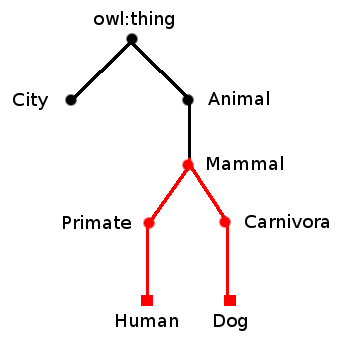
\includegraphics[width=0.5\textwidth]{img/hierarchy_with_classes.png} 
% \caption{Die gemeinsamen Klassen (rot markiert) von \article{Human} und \article{Dog} -- \article{Mammal}, \article{Animal} und \article{owl:Thing} -- liegen alle auf einem Pfad.
% Die Anzahl der Individuen, die diesen Klassen zugehörig sind, entspricht daher der Größe der Klasse \article{Mammal}.}
% \end{figure*}

%Virtuoso SPARQL
\paragraph{Verfahren 2}
Handelt es sich bei der zu verwendenden Hierarchie (wie in Abbildung \ref{fig:monohierarchie_pfad}) um eine Monohierarchie, also um einen Baum, dann existiert ein performanteres Verfahren.
Dabei macht man sich zunutze, dass in einer Monohierarchie jede Instanz höchstens eine direkte Klasse und jede Klasse höchstens eine direkte Oberklasse besitzt. Sämtliche gemeinsamen Klassen liegen daher auf 
einem Pfad und $T$ lässt sich daher darstellen als $T = {t_1,t_2,\ldots,t_e}$ mit  $t_1 \subseteq t_2 \subseteq \ldots \subseteq t_e$ (siehe Abbildung \ref{fig:monohierarchie_pfad}).
Daher gilt $|t_1 \cap t_2 \cap \ldots \cap t_e| = |t_1| = \min(\{|t_1|,|t_2|,\ldots,|t_e|\})$.
%$|\bigcap_{t \in T}  t| = \min(||)$
Da sich die Größe jeder Klasse einer Hierarchie vorberechnen lässt, ist damit die Berechnung der Klassengröße sehr effizient möglich.
\begin{figure*}[h]
\begin{center}
\Tree[2]{
			&\Kred{\article{owl:Thing}}\Vred  \\
\K{\article{City}}	&					&\Kred{\article{Animal}}\Bred{d}\\
			&					&\Kred{\article{Mammal}}\B{dl}\B{dr}\\
			&\Kblue{\article{Carnivora}}\B{d}		&					&\Kblue{\article{Primate}}\B{d}\\
			&\Kblue{\article{Dog}}			&					&\Kblue{\article{Human}}\\
} 
\end{center}
%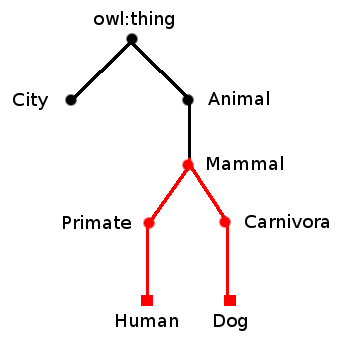
\includegraphics[width=0.5\textwidth]{img/hierarchy_with_classes.png} 
\caption{Die gemeinsamen Klassen \iffalse(rot markiert)\fi von \article{Human} und \article{Dog} -- \article{Mammal}, \article{Animal} und \article{owl:Thing} -- liegen alle auf einem Pfad.
Die Anzahl der Individuen, die diesen Klassen zugehörig sind, entspricht daher der Größe der Klasse \article{Mammal}.}
\label{fig:monohierarchie_pfad}
\end{figure*}

Handelt es sich bei der Hierarchie um eine Polyhierarchie, dann bildet dieses Verfahren immer noch eine obere Schranke für den exakten Wert, denn
$\min(\{|t_1|,|t_2|,\ldots,|t_e|\} \geq |t_1 \cap t_2 \cap \ldots \cap t_e|$.
Ob dieses Verfahren auch bei Polyhierarchien noch akzeptable Werte erzeugt, wird in Abschnitt \ref{sec:evaluierung} evaluiert.

\begin{table*}[h]
\begin{threeparttable}
\begin{tabular}{llll}
\toprule 
Hierarchie		&Typ				&expandiert	&Methode\\
\midrule
DBpedia-Klassen		&Monohierarchie			&\checkmark	&2\\
YAGO			&Polyhierarchie			&		&2 (annähernd)\\
Wikipediakategorien	&annähernd Polyhierarchie	&		&keine\tnote{1}\\
\bottomrule
\end{tabular}
\footnotesize
\begin{tablenotes}
 \item [1] Da die Wikipediakategorien Zyklen enthalten, lassen sie sich nicht zuverlässig expandieren und werden daher nicht verwendet.
\end{tablenotes}

\end{threeparttable}
\end{table*}


% To repeat, there is no 'logical result' of an RDF or RDFS query which 
% would support checking transitive closures. You would need to have 
% something like OWL, or have a rule language added, in order to be 
% even able to say 'transitive'.

% \paragraph{DBpedia-Klassen}
% rdf:type in dbpedia, ist bereits expandiert -> mega hauptmethode
% \paragraph{Wikipediakategorien}
% zu schlechte qualität, (wieso?) fallen ganz weg
% \paragraph{YAGO}
% nicht expandiert, deshalb speedmethode


%                  \Tree{
%                         & \Kred{IP}\Vred \\
%                         \Kblue{NP}\Bblue{d} &&
%                                \Kred{I$’$}\Vred \\
%                         \Tblue{John}& \Kred{I$^{0}$} &&
%   
% 		\Kgray{VP} \Vgray \\
%                         && \Kgreen{t}\Linkblue{ull}&&
%                                     \Kgray{V$’$}\Vgray\\
%                         &&&\Kgray{V$^{0}$}&& \Kgray{NP} }
\iffalse
Der nächste Schritt ist nun, 
Hier tritt nun das Problem auf, dass bei allen benutzten Hierarchien 
Mit einer SPARQL-Anfrage lässt sich 

Bei der Berechnung der Anzahl der Klassen 

ist das n denn überhaupt effizient berechenbar mit SPARQL? und wie geht das genau?
ja, es geht, wenn die klassen in dbpedia schon expandiert sind, sonst geht es nich

denn:
mit sparql fragt man ja nur die direkten klassen ab und nicht inklusive superklassen,
also wenn ich wissen will wer alles animal und säugetier und thing ist, würde mir das ding bei nicht expandierten sachen nicht das pferd zurückgeben wenn da nicht animal mit drinsteht
-> aber für rdf:type erstmal ok (denn da geht es? wenn man "`a"' als property nimmt?)
\fi
\paragraph{Anwendung}
Die hierarchiebasierten Ähnlichkeitsmaße sind besonders für streng organisierte Entitäten, wie \zb Lebewesen geeignet und eignen sich gut für die Identifizierung ähnlicher Konzepte,
jedoch weniger für das Feststellen der generellen Beziehungsstärke (Relatedness).
Tabelle \ref{tab:aehnlichkeitsmass-semantisch-hierarchie-dbpedia} zeigt, dass sämtliche Ähnlichkeitswerte der DBpedia-Hierarchie von den untersuchten Paaren von Lebewesen 
mit der biologischen Ähnlichkeit übereinstimmen. Die vier Paare mit den höchsten Ähnlichkeitswerten sind die Paare der beiden Säugetiere, der Vögel, der Insekten und der Pflanzen.
Da bei den untersuchten Entitäten keine YAGO-Klassenzuordnungen vorlagen, konnten sie damit nicht geprüft werden.
\begin{table}
\begin{tabular}{lll}
\toprule
Konzeptpaar					&Ähnlichkeitswert $\s_{h_d}$\\
\midrule
Wild\_boar		&Pig		&0,9977\\
Ostrich		&Griffon\_Vulture		&0,9964\\
Ant		&Bee		&0,9909\\
Oak		&Willow		&0,9901\\
Wild\_boar		&Ostrich		&0,9746\\
Wild\_boar		&Ant		&0,9746\\
Wild\_boar		&Griffon\_Vulture		&0,9746\\
Wild\_boar		&Bee		&0,9746\\
Pig		&Ostrich		&0,9746\\
Pig		&Ant		&0,9746\\
Pig		&Griffon\_Vulture		&0,9746\\
Pig		&Bee		&0,9746\\
Ostrich		&Ant		&0,9746\\
Ostrich		&Bee		&0,9746\\
Ant		&Griffon\_Vulture		&0,9746\\
Griffon\_Vulture		&Bee		&0,9746\\
Wild\_boar		&Oak		&0,9628\\
Wild\_boar		&Willow		&0,9628\\
Pig		&Oak		&0,9628\\
Pig		&Willow		&0,9628\\
Ostrich		&Oak		&0,9628\\
Ostrich		&Willow		&0,9628\\
Ant		&Oak		&0,9628\\
Ant		&Willow		&0,9628\\
Griffon\_Vulture		&Oak		&0,9628\\
Griffon\_Vulture		&Willow		&0,9628\\
Bee		&Oak		&0,9628\\
Bee		&Willow		&0,9628\\
\bottomrule
\end{tabular}
\caption{Werte der Ähnlichkeitsfunktion $\s_{h_d}$ von einigen Lebewesen}
\label{tab:aehnlichkeitsmass-semantisch-hierarchie-dbpedia}
\end{table}


\FloatBarrier
\begin{Huge}---------------------------------------------------------------------------------------Der Abgrund------------------------------------------------------------------------------------------------\end{Huge}
\section{Evaluierung}\label{sec:evaluierung}
In diesem Abschnitt wird die Disambiguierungsleistung gemessen und optimiert.
Zunächst wird anhand eines einfachen Beispiels das verwendete Verfahren beschrieben. %außerhalb des Gesamtsystems von NLP2RDF getestet. der Ähnlichkeit des Abstracts 
Im Anschluß wird die Performance mit den einzelnen Ähnlichkeitsfunktionen und verschiedenen Mappings auf den Testdaten von \citet{cucerzan2007}, die auch in Abschnitt \ref{relatedwork} beschrieben sind, gemessen, wobei verschiedene Parameter variiert und deren optimale Werte bestimmt werden.
Schließlich wird eine optimale Kombination der einzelnen Ähnlichkeitsmaße bestimmt.
%dabei wird dann auch parametertuning betrieben bei dem genetischen algorithmus bei den abstracts, da war das ja noch nicht so ganz klar
%die anderen ähnlichkeitsmaße sind eigentlich good to go, obwohl man die art der gewichtung mit frequenzklasse und so sowohl beim abstract als auch bei dne properties variiern könnte
%dann wird noch geguckt was es bringt die maße zu verbinden denn die letzten 2 sind halt (davon das letzte noch mehr) so sure shot methoden die echt gute werte bringen aber halt nur wenn uach ne infobox da ist was natürlich klar ist bei dbpedia

\begin{bsp}
 %Gegeben sei folgender Beispielsatz:
\emph{\begin{quote}You can set a common nail’s head below the surface without smashing the surrounding wood with your hammer---just use another nail.\footnotemark{}\end{quote}}
\footnotetext{\url{http://www.popularmechanics.com/blogs/home_journal_news/4217164.html}, Artikel vom \datum{2007}{5}{24}, aufgerufen am \datum{2010}{2}{1}}

%Anhand dieses Beispielsatzes wird das verwendete Prinzip 
%Die Disambiguierung wurde zunächst mit der Ähnlichkeit des Abstracts außerhalb des Gesamtsystems von NLP2RDF getestet.
%Als einfache Emulation von NLP2RDF %
In diesem Beispielsatz sind manuell die Substantive des Satzes und einige Kandidaten bestimmt, siehe Tabelle \ref{tab:evaluierung_beispielsatz}.
Sowohl die jeweils \textbf{intuitiv} als auch die unter Verwendung des Ähnlichkeitsmaßes des Abstracts \ovalbox{automatisch} eingestuften Bedeutungen sind dabei markiert.
Dabei werden die vorläufigen Parameter verwendet, siehe Tabelle \ref{tab:aehnlichkeitsmass-parameter}.

\begin{table}[htb]
\begin{center}
\begin{tabular}[c]{llll}
\toprule
Wort	&Bedeutungen\\
\midrule
nail	&\ovalbox{\textbf{Nail\_(fastener)}}	&Nail\_(unit)\\
head	&\ovalbox{Head}				&Drumhead\\
surface	&\ovalbox{\textbf{Surface}}		&Surface\_(TV\_series)	&Surface\_wave\\
wood	&\ovalbox{\textbf{Wood}}		&USS\_Wood		&Wood\_(golf)\\
hammer	&\ovalbox{\textbf{Hammer}}		&MC\_Hammer\\
nail	&\ovalbox{\textbf{Nail\_(fastener})}	&Nail\_(unit)\\
\bottomrule
\end{tabular}
\end{center}
\caption{Ergebnis der automatischen und menschlichen Disambiguierung}
\label{tab:evaluierung_beispielsatz}
\end{table}

%Nail_(fastener), Head, Surface_wave, Wood, Hammer, Nail_(fastener)
%[Nail_(fastener), Head, Surface, Wood_(golf), Hammer, Nail_(fastener)]
\begin{sidewaystable}
%\footnotesize
\begin{tabular}{llllllllllll}
~	&\begin{sideways}Nail\_(fastener)\end{sideways}	&\begin{sideways}Drumhead\end{sideways}	&\begin{sideways}Surface\_wave\end{sideways}	&\begin{sideways}Head\end{sideways}	&\begin{sideways}USS\_Wood\end{sideways}	&\begin{sideways}Hammer\end{sideways}	&\begin{sideways}Wood\_(golf)\end{sideways}	&\begin{sideways}Surface\end{sideways}	&\begin{sideways}Wood\end{sideways}	&\begin{sideways}MC\_Hammer\end{sideways}	&\begin{sideways}Surface\_(TV\_series)\end{sideways}\\
\midrule
Drumhead	&\val{0.0582}	&~	&~	&~	&~	&~	&~	&~	&~	&~	&~\\

Surface\_wave	&\val{0.0708}	&\val{0.0554}	&~	&~	&~	&~	&~	&~	&~	&~	&~\\

Head	&\val{0.0661}	&\val{0.0273}	&\val{0.0855}	&~	&~	&~	&~	&~	&~	&~	&~\\

USS\_Wood	&\val{0.0389}	&\val{0.0151}	&\val{0.0176}	&\val{0.0312}	&~	&~	&~	&~	&~	&~	&~\\

Hammer	&\val{0.1734}	&\val{0.0493}	&\val{0.082}	&\val{0.0926}	&\val{0.0673}	&~	&~	&~	&~	&~	&~\\

Wood\_(golf)	&\val{0.0845}	&\val{0.0547}	&\val{0.0681}	&\val{0.0747}	&\val{0.0194}	&\val{0.1128}	&~	&~	&~	&~	&~\\

Surface	&\val{0.0857}	&\val{0.0374}	&\val{0.1334}	&\val{0.0467}	&\val{0.0145}	&\val{0.0991}	&\val{0.0364}	&~	&~	&~	&~\\

Wood	&\val{0.1322}	&\val{0.0496}	&\val{0.0633}	&\val{0.0533}	&\val{0.0982}	&\val{0.1239}	&\val{0.1438}	&\val{0.0972}	&~	&~	&~\\

MC\_Hammer	&\val{0.0425}	&\val{0.0276}	&\val{0.0302}	&\val{0.0251}	&\val{0.0149}	&\val{0.0675}	&\val{0.0326}	&\val{0.0485}	&\val{0.0755}	&~	&~\\

Surface\_(TV\_series)	&\val{0.0474}	&\val{0.0419}	&\val{0.0344}	&\val{0.0305}	&\val{0.0659}	&\val{0.0648}	&\val{0.0333}	&\val{0.0718}	&\val{0.0595}	&\val{0.0807}	&~\\

Nail\_(unit)	&\val{0.1507}	&\val{0.0574}	&\val{0.0787}	&\val{0.0661}	&\val{0.0267}	&\val{0.1144}	&\val{0.0608}	&\val{0.0462}	&\val{0.0713}	&\val{0.0484}	&\val{0.0352}\\
\bottomrule
\end{tabular}
\caption{Die Werte der Basisähnlichkeitsfunktion für alle möglichen Paare von Bedeutungen der Substantive des Beispielsatzes}
\label{evaluierung_beispielsatz_werte}
\iffalse
\begin{tabular}{lllllllllllll}
~	&\begin{sideways}Nail\_(fastener)\end{sideways}	&\begin{sideways}Drumhead\end{sideways}	&\begin{sideways}Surface\_wave\end{sideways}	&\begin{sideways}Head\end{sideways}	&\begin{sideways}USS\_Wood\end{sideways}	&\begin{sideways}Hammer\end{sideways}	&\begin{sideways}Wood\_(golf)\end{sideways}	&\begin{sideways}Surface\end{sideways}	&\begin{sideways}Wood\end{sideways}	&\begin{sideways}MC\_Hammer\end{sideways}	&\begin{sideways}Surface\_(TV\_series)\end{sideways}	&Nail\_(unit)\\
\midrule
Nail\_(fastener)	&null	&\val{0.0582}	&\val{0.0708}	&\val{0.0661}	&\val{0.0389}	&\val{0.1734}	&\val{0.0845}	&\val{0.0857}	&\val{0.1322}	&\val{0.0425}	&\val{0.0474}	&\val{0.1507}\\
Drumhead	&null	&null	&\val{0.0554}	&\val{0.0273}	&\val{0.0151}	&\val{0.0493}	&\val{0.0547}	&\val{0.0374}	&\val{0.0496}	&\val{0.0276}	&\val{0.0419}	&\val{0.0574}\\
Surface\_wave	&null	&null	&null	&\val{0.0855}	&\val{0.0176}	&\val{0.082}	&\val{0.0681}	&\val{0.1334}	&\val{0.0633}	&\val{0.0302}	&\val{0.0344}	&\val{0.0787}\\
Head	&null	&null	&null	&null	&\val{0.0312}	&\val{0.0926}	&\val{0.0747}	&\val{0.0467}	&\val{0.0533}	&\val{0.0251}	&\val{0.0305}	&\val{0.0661}\\
USS\_Wood	&null	&null	&null	&null	&null	&\val{0.0673}	&\val{0.0194}	&\val{0.0145}	&\val{0.0982}	&\val{0.0149}	&\val{0.0659}	&\val{0.0267}\\
Hammer	&null	&null	&null	&null	&null	&null	&\val{0.1128}	&\val{0.0991}	&\val{0.1239}	&\val{0.0675}	&\val{0.0648}	&\val{0.1144}\\
Wood\_(golf)	&null	&null	&null	&null	&null	&null	&null	&\val{0.0364}	&\val{0.1438}	&\val{0.0326}	&\val{0.0333}	&\val{0.0608}\\
Surface	&null	&null	&null	&null	&null	&null	&null	&null	&\val{0.0972}	&\val{0.0485}	&\val{0.0718}	&\val{0.0462}\\
Wood	&null	&null	&null	&null	&null	&null	&null	&null	&null	&\val{0.0755}	&\val{0.0595}	&\val{0.0713}\\
MC\_Hammer	&null	&null	&null	&null	&null	&null	&null	&null	&null	&null	&\val{0.0807}	&\val{0.0484}\\
Surface\_(TV\_series)	&null	&null	&null	&null	&null	&null	&null	&null	&null	&null	&null	&\val{0.0352}\\
Nail\_(unit)	&null	&null	&null	&null	&null	&null	&null	&null	&null	&null	&null	&null\\
\end{tabular}
\fi
\iffalse
\begin{tabular}{llllllllllll}

\val{0.0582}	&\val{0.0708}	&\val{0.0661}	&\val{0.0389}	&\val{0.1734}	&\val{0.0845}	&\val{0.0857}	&\val{0.1322}	&\val{0.0425}	&\val{0.0474}	&\val{0.1507}\\
~	&\val{0.0554}	&\val{0.0273}	&\val{0.0151}	&\val{0.0493}	&\val{0.0547}	&\val{0.0374}	&\val{0.0496}	&\val{0.0276}	&\val{0.0419}	&\val{0.0574}\\
~	&~	&\val{0.0855}	&\val{0.0176}	&\val{0.082}	&\val{0.0681}	&\val{0.1334}	&\val{0.0633}	&\val{0.0302}	&\val{0.0344}	&\val{0.0787}\\
~	&~	&~	&\val{0.0312}	&\val{0.0926}	&\val{0.0747}	&\val{0.0467}	&\val{0.0533}	&\val{0.0251}	&\val{0.0305}	&\val{0.0661}\\
~	&~	&~	&~	&\val{0.0673}	&\val{0.0194}	&\val{0.0145}	&\val{0.0982}	&\val{0.0149}	&\val{0.0659}	&\val{0.0267}\\
~	&~	&~	&~	&~	&\val{0.1128}	&\val{0.0991}	&\val{0.1239}	&\val{0.0675}	&\val{0.0648}	&\val{0.1144}\\
~	&~	&~	&~	&~	&~	&\val{0.0364}	&\val{0.1438}	&\val{0.0326}	&\val{0.0333}	&\val{0.0608}\\
~	&~	&~	&~	&~	&~	&~	&\val{0.0972}	&\val{0.0485}	&\val{0.0718}	&\val{0.0462}\\
~	&~	&~	&~	&~	&~	&~	&~	&\val{0.0755}	&\val{0.0595}	&\val{0.0713}\\
~	&~	&~	&~	&~	&~	&~	&~	&~	&\val{0.0807}	&\val{0.0484}\\
~	&~	&~	&~	&~	&~	&~	&~	&~	&~	&\val{0.0352}\\
\end{tabular}
\fi
\end{sidewaystable}

Tabelle \ref{tab:evaluierung_beispielsatz} zeigt, dass der Algorithmus mit der intuitiven Einschätzung in diesem Fall exakt übereinstimmt.
Der Begriff \emph{head} als \emph{Nagelkopf} war zur Zeit der Evaluierung in Wikipedia nicht vorhanden, es gibt bei diesem Begriff also keine richtige Bedeutung.
%Ähnlichkeitsfunktionen
\end{bsp}

Im Folgenden wird die Disambiguierung anhand der Testdaten aus \cite{cucerzan2007} ausgewertet.
Von den dort enhaltenen 797 Oberflächenformen lassen sich 651 (\valunit{81.6813}{\%}) zu einem Wikipediaartikel zuordnen und sind damit disambiguierbar.
Die Parameter des verwendeten Disambiguierungsalgorithmus (siehe Abschnitt \ref{sec:algorithmus}) werden empirisch festgelegt, indem die Parameter varriert und das Optimum bestimmt wird.
Das in Abschnitt \ref{sec:mapping1} erstellte erste Mapping ist für diesen Zweck jedoch nicht geeignet, da es auf hohe Präzision ausgelegt ist, was jedoch zu Lasten der Kandidatenvielfalt geht.
Außerdem enhalten die Testdaten, im Gegensatz zu Tabelle \ref{tab:evaluierung_beispielsatz}, einen hohen Anteil an Mehrfachwörtern, also Verbindungen mehrerer Wörter, \zb{} \emph{SPD Vorsitzender Frank Walter Steinmeier},
die benutzte Wortschatzdatei enhält jedoch nur einzelne Wörter.
Dies macht ein neues Mapping notwendig:

\paragraph{Zweites Mapping}

Das zweite Mapping wird mit den folgenden Stringtransformatoren in dieser Reihenfolge erzeugt:

\begin{center}
\begin{tabular}{ll}
\toprule
Stringtransformator				&Beispielergebnis\\
\midrule
						&Der Baum im Wald (Film)\\
entferne Klammerpaare und ihren Inhalt		&Der Baum im Wald\\
zerlege das Wort in seine Teilwörter		&$\{\textnormal{Der}, \textnormal{Baum}, \textnormal{im}, \textnormal{Wald}\}$\\
entferne Wörter mit weniger als drei Buchstaben	&$\{\textnormal{Der}, \textnormal{Baum}, \textnormal{Wald}\}$\\
schreibe den ersten Buchstaben klein		&$\{\textnormal{der}, \textnormal{baum}, \textnormal{wald}\}$\\
\bottomrule
\end{tabular}
\end{center}

Weiterhin werden dem Mapping noch alle Paare $(w,a)$ hinzugefügt, bei denen $w$ der Titel einer Entität ist, die die Entität $a$ disambiguiert, oder per Redirect auf $a$ verweist:

\begin{center}
\begin{tabular}{ll}
\toprule
Herr der Ringe		&Der\_Herr\_der\_Ringe\_(Film)\\
Der Herr der Ringe	&Der\_Herr\_der\_Ringe\_(Film)\\
Der Herr der Ringe	&Der\_Herr\_der\_Ringe\_(Buch)\\
%\midrule
\bottomrule
\end{tabular}
\end{center}

Die Standardwerte für die nicht variierten Parameter sind:

\begin{center}
\begin{tabular}{ll}
\toprule
cooling Factor			&0.9\\
Anzahl der Iterationen $n$	&1000\\
Anfangstemperatur		&1000\\
%\midrule
\bottomrule
\end{tabular}
\end{center}

Die Basis $a$ der Distanzfunktion $a^{d_{ij}}$ ist nicht mit angegeben, da die zugrundeliegenden Vergleichsdaten nur die Wörter ohne Satzposition enhalten und damit sämtliche Wörter als im selben Satz befindlich
 behandelt werden.
Die resultierenden Genauigkeiten der Disambiguierung mit der Ähnlichkeitsfunktion der Abstracts sind in den Abbildungen 
\ref{fig:disambiguierung_evaluierung_mapping2_n}, \ref{fig:disambiguierung_evaluierung_mapping2_cooling_factor} und \ref{fig:disambiguierung_evaluierung_mapping2_starting_temperature} dargestellt.

\begin{figure}[tbh]
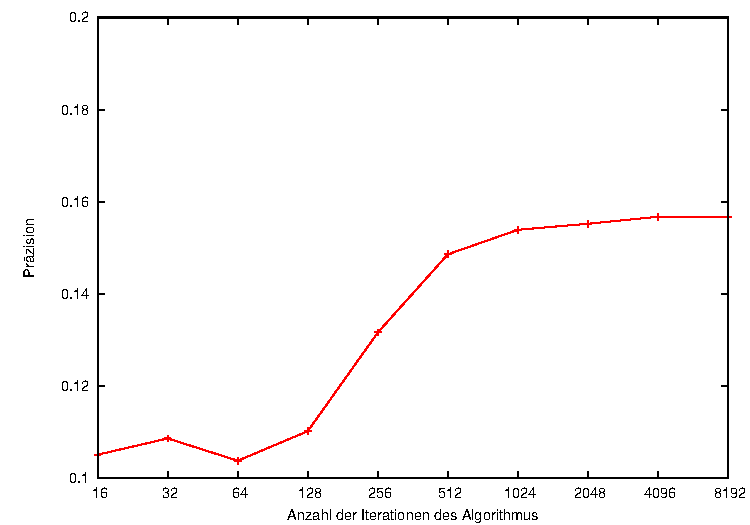
\includegraphics[height=0.4\textheight]{img/pdf/mapping2/n.pdf}
\caption[]{Disambiguierungspräzision mit dem zweiten Mapping und der Ähnlichkeitsfunktion der Abstracts in Abhängigkeit der Anzahl der Iterationen}
\label{fig:disambiguierung_evaluierung_mapping2_n}
\end{figure}

\begin{figure}[tbh]
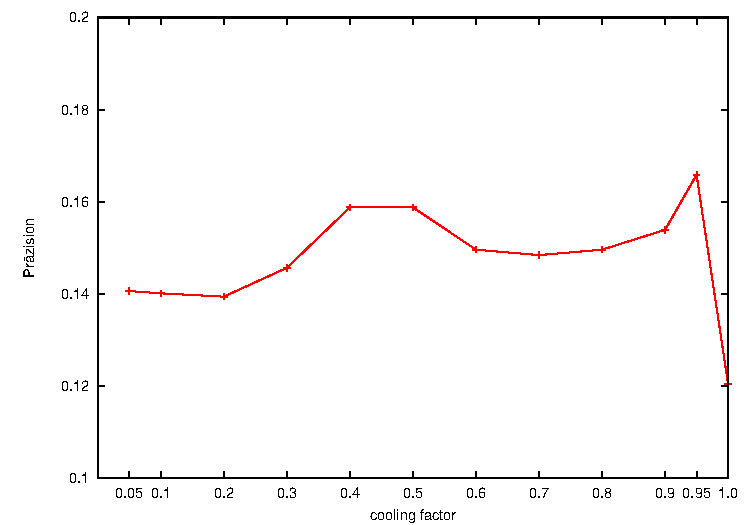
\includegraphics[height=0.4\textheight]{img/pdf/mapping2/cooling_factor.pdf}
\caption[]{Disambiguierungspräzision mit dem zweiten Mapping und der Ähnlichkeitsfunktion der Abstracts in Abhängigkeit des cooling factors}
\label{fig:disambiguierung_evaluierung_mapping2_cooling_factor}
\end{figure}

\begin{figure}[tbh]
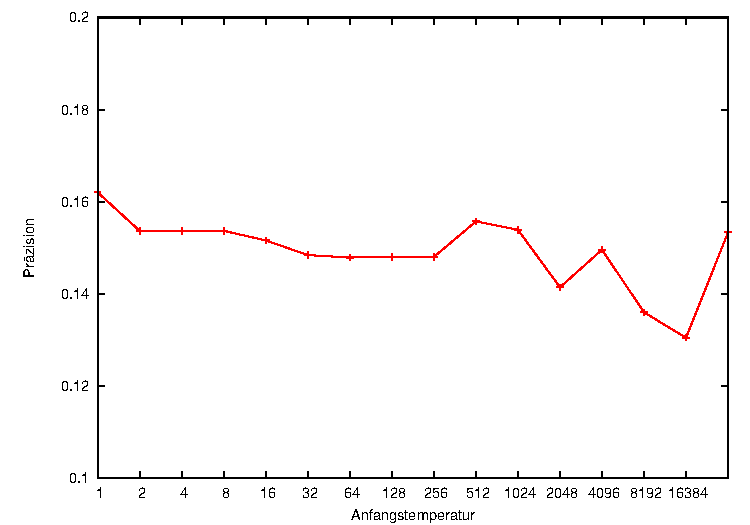
\includegraphics[height=0.4\textheight]{img/pdf/mapping2/starting_temperature.pdf}
\caption[]{Disambiguierungspräzision mit dem zweiten Mapping und der Ähnlichkeitsfunktion der Abstracts in Abhängigkeit der Anfangstemperatur}
\label{fig:disambiguierung_evaluierung_mapping2_starting_temperature}
\end{figure}

Aufgrund der Vielzahl an Kandidaten sind die Resultate des zweiten Mappings ungenügend für eine erfolgreiche Disambiguierung, selbst wenn man bedenkt, dass nur eine einzelne Ähnlichkeitsfunktion verwendet wird.
Wegen der sehr niedrigen Werte ist auch der Wert für die Analyse der Parameter fraglich.
Aus diesen Gründen wurde ein drittes Mapping erzeugt:
%Trotzdem lassen sich generelle Trends für die Parameter beobachten und damit neue Standardwerte festlegen.
%Da der verwendete Algorithmus Zufallswerte verwendet und die Abweichungen sehr gering sind, werden diese jedoch mit dem dritten Mapping noch einmal überprüft.
% Die überarbeiteten Standardwerte sind:
% \begin{center}
% \begin{tabular}{ll}
% \toprule
% cooling Factor			&0.95\\
% Anzahl der Iterationen $n$	&1000\\
% Anfangstemperatur		&32000\\
% %\midrule
% \bottomrule
% \end{tabular}
% \end{center}

\FloatBarrier
\paragraph{Drittes Mapping}

%Um eine annehmbare Präzision zu erreichen, wird nun ein drittes Mapping verwendet.
%Hierzu wurde freundlicherweise von Herrn Volker Böhlke vom Wortschatzprojekt eine Mehrfachwortliste zur Verfügung gestellt.
%Das dritte Mapping wird mit den folgenden Stringtransformatoren in dieser Reihenfolge erzeugt:
Um dieses Mapping zu erzeugen, wird im Gegensatz zu den anderen beiden Mappings nicht Wortschatz2DBpedia benutzt, sondern es werden nur die folgenden Wikipediadaten verwendet:
\begin{itemize}
\item Titel
\item Redirects
\item Disambiguierungen
\end{itemize}

Dies hat den Vorteil, dass nur relevante Kandidaten erzeugt werden und die Kandidatenanzahl nicht zu groß wird aber auch den Nachteil, dass keine Matches von einzelnen Wörtern auf Mehrwörter möglich sind, wenn diese nicht in Form eines Redirects oder einer Disambiguierung vorliegen.
Dieses Problem wird jedoch in den meisten Fällen umgangen, in dem bei der Verwendung des dritten Mappings im selben Text befindliche Oberflächenformen, die nur aus einem Wort bestehen, durch die Kandidaten derer erweitert werden,
die aus mehreren Wörtern bestehen, von denen mindestens eines mit dem einzelnen Wort übereinstimmt. Wird beispielsweise in einem Text \emph{Barack Obama} referenziert, dann wird der Kandidat \article{Barack_Obama} jedem
Vorkommen von \emph{Barack} und \emph{Obama} in diesem Text hinzugefügt.

% \begin{center}
% \begin{tabular}{ll}
% \toprule
% \midrule
% 
% \bottomrule
% \end{tabular}
% \end{center}

%Weiterhin werden dem Mapping noch alle Paare $(w,a)$ hinzugefügt, \todo{...} %bei denen $w$ der Titel einer Entität ist, die die Entität $a$ disambiguiert, oder per Redirect auf $a$ verweist:

Die Präzisionen der Disambiguierung mit dem Ähnlichkeitsmaß der Abstracts mit dem dritten Mapping in Abhängigkeit der überarbeiten Standardparameter sind in den Abbildungen
\ref{fig:disambiguierung_evaluierung_mapping3_n}, \ref{fig:disambiguierung_evaluierung_mapping3_cooling_factor} und \ref{fig:disambiguierung_evaluierung_mapping3_starting_temperature} dargestellt.
Daraus wurden die endgültigen Parameter für den Disambiguierungsalgorithmus abgeleitet:

\begin{center}
\begin{tabular}{ll}
\toprule
cooling Factor			&0.9\\
Anzahl der Iterationen $n$	&4096\\
Anfangstemperatur		&8192\\
%\midrule
\bottomrule
\end{tabular}
\end{center}

\begin{figure}[tbh]
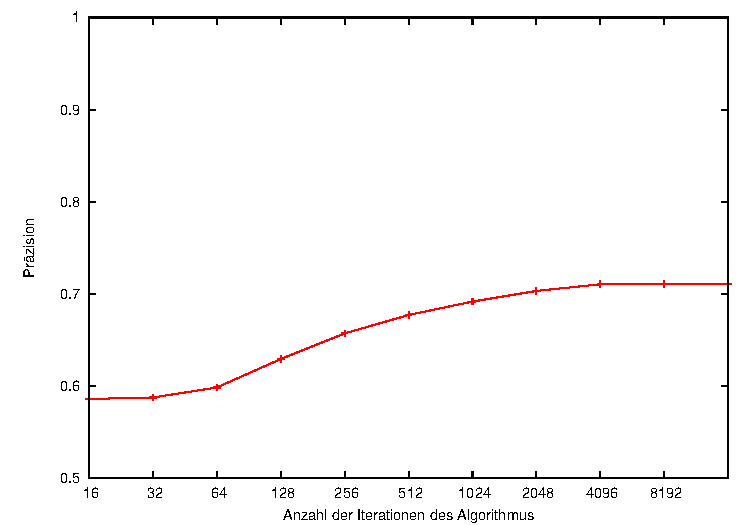
\includegraphics[height=0.4\textheight]{img/pdf/mapping3/n.pdf}
\caption[]{Disambiguierungspräzision mit dem dritten Mapping und der Ähnlichkeitsfunktion der Abstracts in Abhängigkeit der Anzahl der Iterationen}
\label{fig:disambiguierung_evaluierung_mapping3_n}
\end{figure}

\begin{figure}[tbh]
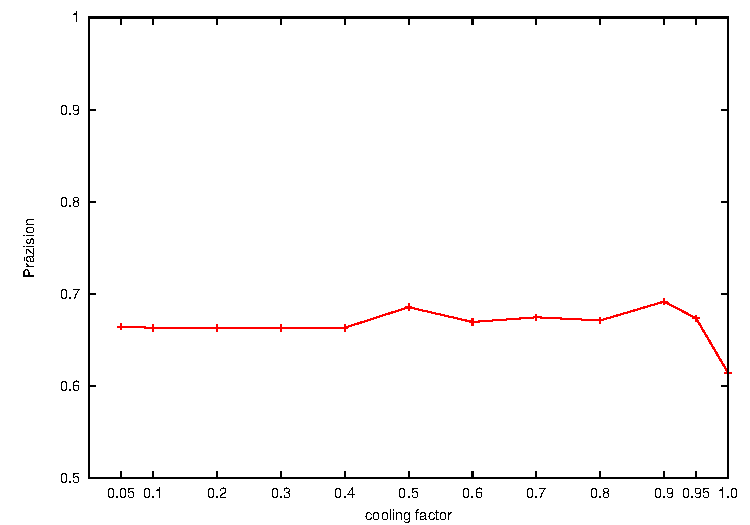
\includegraphics[height=0.4\textheight]{img/pdf/mapping3/cooling_factor.pdf}
\caption[]{Disambiguierungspräzision mit dem dritten Mapping und der Ähnlichkeitsfunktion der Abstracts in Abhängigkeit des cooling factors}
\label{fig:disambiguierung_evaluierung_mapping3_cooling_factor}
\end{figure}

\begin{figure}[tbh]
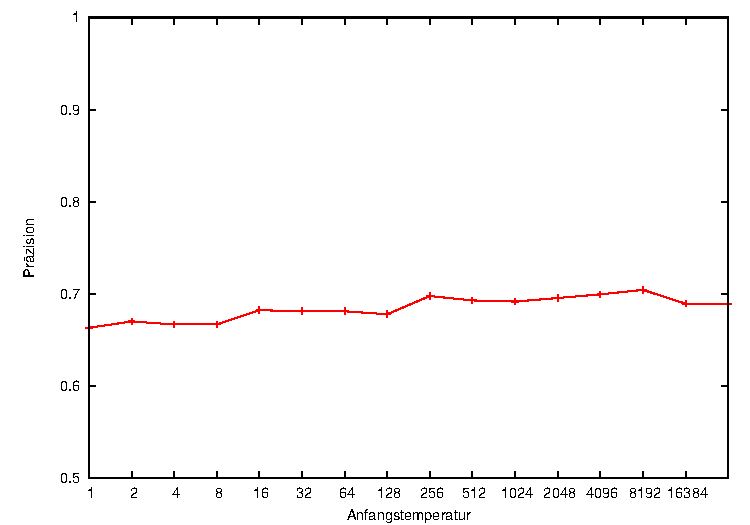
\includegraphics[height=0.4\textheight]{img/pdf/mapping3/starting_temperature.pdf}
\caption[]{Disambiguierungspräzision mit dem dritten Mapping und der Ähnlichkeitsfunktion der Abstracts in Abhängigkeit der Anfangstemperatur}
\label{fig:disambiguierung_evaluierung_mapping3_starting_temperature}
\end{figure}

% \begin{figure}[tbh]
% 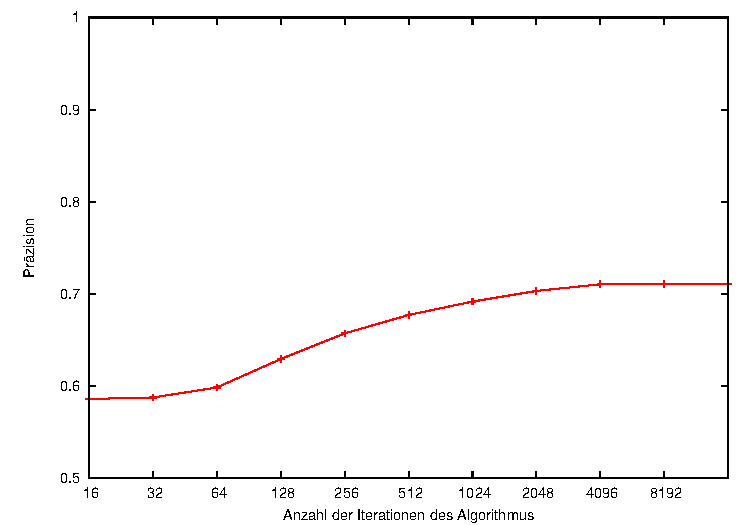
\includegraphics[width=1\textwidth]{img/pdf/mapping3/n.pdf}
% \caption[]{Disambiguierungspräzision mit dem dritten Mapping und der Ähnlichkeitsfunktion der Abstracts in Abhängigkeit der Anzahl der Iterationen}
% \label{fig:disambiguierung_evaluierung_mapping3_n}
% \end{figure}
% 
% \begin{figure}[tbh]
% 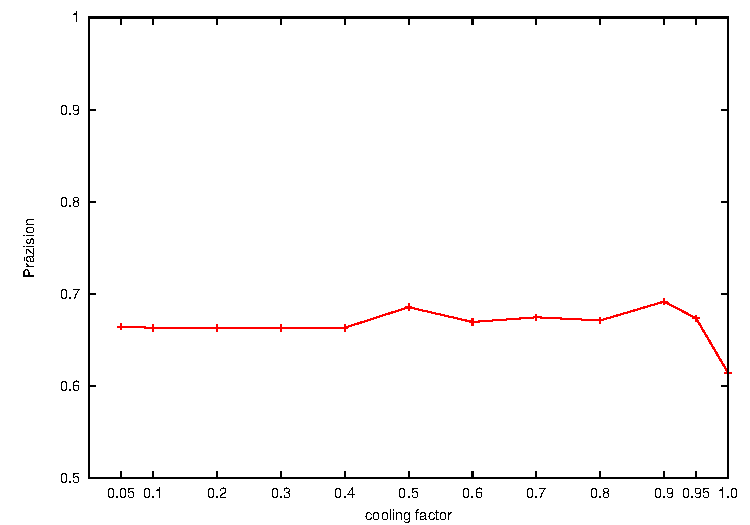
\includegraphics[width=1\textwidth]{img/pdf/mapping3/cooling_factor.pdf}
% \caption[]{Disambiguierungspräzision mit dem dritten Mapping und der Ähnlichkeitsfunktion der Abstracts in Abhängigkeit des cooling factors}
% \label{fig:disambiguierung_evaluierung_mapping3_cooling_factor}
% \end{figure}
% 
% \begin{figure}[tbh]
% 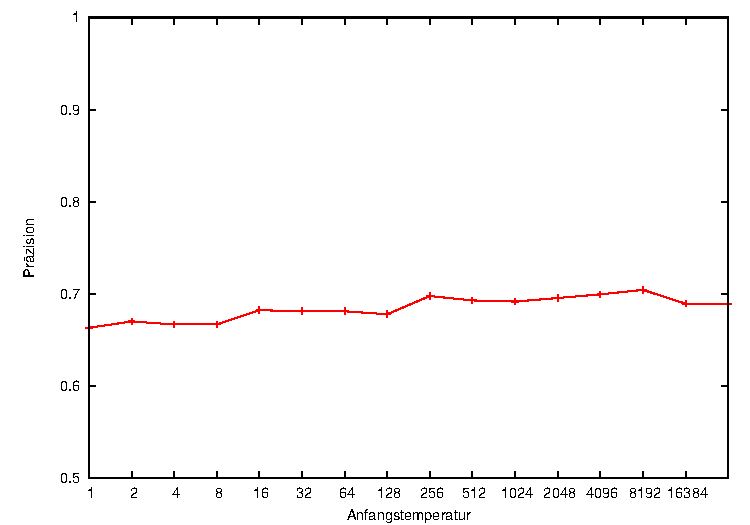
\includegraphics[width=1\textwidth]{img/pdf/mapping3/starting_temperature.pdf}
% \caption[]{Disambiguierungspräzision mit dem dritten Mapping und der Ähnlichkeitsfunktion der Abstracts in Abhängigkeit der Anfangstemperatur}
% \label{fig:disambiguierung_evaluierung_mapping3_starting_temperature}


Im Folgenden wird untersucht, welche Kombination der Ähnlichkeitsmaße optimal ist.

\begin{center}
\begin{tabular}{ll}
\toprule
Ähnlichkeitsmaß		&Formelzeichen\\
\midrule
Abstracts			&$\s_{a}$\\
Properties (Version 1)		&$\s_{p}$\\
Properties (Version 2)		&$\s_{p_2}$\\
DBpedia-Hierarchie		&$\s_{h_d}$\\
YAGO-Hierarchie			&$\s_{h_y}$\\
%Hierarchie gemischt		&$\s_{h}= \average(\s_{h_d}, \s_{h_y})$\\
\bottomrule
\end{tabular}
\end{center}

\begin{table}
\begin{tabular}{ll}
\toprule
Kombination	&Präzision\\
\midrule
Grundlinie							&\valunit{57.6651}{\%}\\
$\s_{a}$							&\valunit{71.9453}{\%}\\
$\s_{p}$							&\valunit{67.1732}{\%}\\
$\s_{p_2}$							&\valunit{70.7144}{\%}\\
$\s_{h_d}$							&\valunit{67.5798}{\%}\\
$\s_{h_y}$							&\valunit{66.0609}{\%}\\
%$\s_{h}$							&0.5154\\
$\average(\s_{a},\s_{p_2},\s_{h_d},\s_{h_y})$			&\valunit{68.3502}{\%}\\
$\average'(\s_{a},\s_{p_2},\s_{h_d},\s_{h_y})$			&\valunit{64.8386}{\%}\\
$\average''(\s_{a},\s_{p_2},\s_{h_d},\s_{h_y})$			&\valunit{65.9421}{\%}\\
$\average'''(\s_{a},\s_{p_2},\s_{h_d},\s_{h_y})$		&\valunit{71.3748}{\%}\\
$\max'(\s_{a},\s_{p_2},\s_{h_d},\s_{h_y})$			&\valunit{72.1956}{\%}\\
%gewichtetes Maximum : 72.1956
%$\average_{\textnormal{geom}}(\s_{a},\s_{p_2},\s_{h_d})$	&\\
%$\max(\s_{a},\s_{p_2},\s_{h_d})$				&\valunit{}{\%}\\
\bottomrule
\end{tabular}
\caption{Kombinationen verschiedener Ähnlichkeitsmaße und deren Präzision}
\label{tab:disambiguierung_evaluierung_kombination}
\end{table}

Tabelle \ref{tab:disambiguierung_evaluierung_kombination} zeigt, dass sich unter Verwendung des Ähnlichkeitsmaßes der Abstracts bereits eine Präzision von \valunit{71.9453}{\%} erreichen lässt,
was eine signifikante Steigerung gegenüber der Grundlinie von \valunit{57.6651}{\%} ist.
Die Grundlinie wird ermittelt, in dem als Ähnlichkeitsmaß die konstante Funktion $s(x,y) = 1$ verwendet wird, wodurch die Kandidatenauswahl also zufällig erfolgt.
Aufgrund der großen Anzahl von 651 disambiguierbaren Oberflächenformen sind zufällige Schwankungen dabei vernachlässigbar.
Dass dabei bereits ein Wert von \valunit{57.6651}{\%} erreicht wird erklärt sich damit, dass 375 der 651 disambiguierbaren Oberflächenformen nur einen einzigen Kandidaten aufweisen (siehe Abbildung \ref{fig:disambiguierung_evaluierung_candidatenumbers}).
Werden die semantischen Ähnlichkeitsmaße einzeln verwendet, ergibt sich eine niedrigere Genauigkeit als unter Verwendung des textbasierten Ähnlichkeitsmaß der Abstracts.
Dies wird damit erklärt, dass nur für einen Teil der Entitäten semantische Daten verfügbar sind.
Tabelle \ref{tab:disambiguierung_evaluierung_nicht_null_werte} zeigt die Anzahl der beim Testen verglichenen Entitätspaare und den Anteil der Paare, die keine Nullwerte liefern.
Die Präzision, die durch die Verwendung des kombinierten Ähnlichkeitsmaßes in Form des arithmetische Mittels der Ähnlichkeitsmaße $\s_{a}$,$\s_{p_2}$,$\s_{h_d}$ und $\s_{h_y}$
erreicht wird, ist mit \valunit{68.3502}{\%} jedoch deutlich geringer als die die durch $\s_{a}$ erreichte von \valunit{71.9453}{\%}, obwohl die Präzisionen der semantischen Ähnlichkeitsmaße deutlich über der Grundlinie liegen und eine
höhere Präzision durch die Integration der verschiedenen Maße erwartet wurde.
Eine mögliche Erklärung dafür ist, dass Paare mit verfügbaren semantischen Daten gegenüber denen ohne solche Daten durch die Disambiguierung bevorzugt werden.
Aus diesem Grund wird zusätzlich zum arithmetischen Mittel $\average$ auch ein erweitertes Mittel $\average'$ verwendet, welches sämtliche Nullwerte durch die in Tabelle \ref{tab:disambiguierung_evaluierung_durchschnittswerte}
aufgeführten Werte ersetzt, welche die Durchschnittswerte aller während eines Testlaufes ermittelten Werte der Ähnlichkeitsfunktionen, wobei Nullwerte ausgenommen sind, darstellen.
Mit diesem Verfahren werden Entitätspaare, bei denen beide Elemente keine semantischen Daten gemeinsamer Art aufweisen (Properties, YAGO-Klassenzuordnungen oder DBpedia-Klassenzuordnungen) nicht mehr gegenüber
den Anderen benachteiligt, andererseits werden jedoch Paare, die zwar über diese Daten verfügen, jedoch in gar keinem Merkmal übereinstimmen, nicht korrekt abgestraft.
% -> verbesserung: mit "`null"' und "`0"' rückgabewert auf Double statt double setzen und dann da variieren
%Dieses Mittel basiert auf der Annahme, dass einander unähnliche Entitäten in vielen Fällen zwar sehr kleine, jedoch keine Nullwerte annehmen, solange semantische Daten verfügbar sind.
Die Präzision, die durch Verwendung von $\average'$ erreicht wird, liegt mit \valunit{64.8386}{\%} jedoch noch unter der mit $\average$ Erreichten. %} ...
Ein weitere Möglichkeit der Kombination ist das gewichtete Mittel. $\average''$ entsteht durch die Gewichtung jedes Wertes mit dem Kehrwert seines Durchschnittes, wobei Nullwerte wie in $\average'$ durch 
Durchschnittswerte ersetzt werden. Der daraus resultierende Wert von \valunit{65.9421}{\%} liegt zwischen $\average$ und $\average'$, was nahelegt, dass die Mittelung eine Verbesserung der Präzision mit sich bringt,
die Ersetzung von Nullwerten jedoch nicht. Aus diesem Grund ist in Tabelle \ref{tab:disambiguierung_evaluierung_kombination} als weitere Kombination das gewichtete Mittel ohne Nullwertersetzung $\average'''$ aufgeführt,
welches mit \valunit{71.3748}{\%} bessere Werte als $\average$ jedoch immer noch Schlechtere als $\s_a$ erreicht. Die einzige getestete Kombination, die eine Verbesserung gegenüber dem Ähnlichkeitsmaß des Abstracts erreicht 
ist das gewichtete Maximum $\max'$, bei dem vor dem Bilden des Maximums jeder Wert wie bei $\average''$ und $\average'''$ mit dem Kehrwert seines Durchschnittswertes multipliziert wird.
Der durch $\max'$ erreichte Wert liegt mit \valunit{72.1956}{\%} jedoch nur sehr geringfügig über der von $s_a$ erreichten Präzision von \valunit{71.3748}{\%}.




\begin{figure}[tbh]
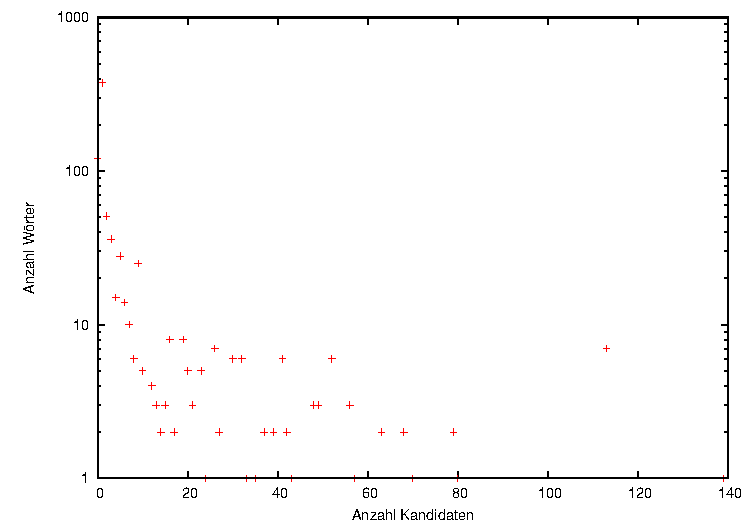
\includegraphics[height=0.4\textheight]{img/pdf/candidatenumbers.pdf}
\caption[]{Verteilung der Anzahl der Bedeutungskandidaten der Oberflächenformen}
\label{fig:disambiguierung_evaluierung_candidatenumbers}
\end{figure}

\begin{table}
\begin{tabular}{llll}
\toprule
Ähnlichkeitsmaß		&Anzahl nicht-null-Werte	&Anteil nicht-null-Werte\\
\midrule
Abstracts			&\val{46490}		&\valunit{71.6300}{\%}\\
Properties (Version 2)		&\val{9194}		&\valunit{14.1658}{\%}\\
DBpedia-Hierarchie		&\val{6206}		&\valunit{9.5620}{\%}\\
YAGO-Hierarchie			&\val{17172}		&\valunit{26.4579}{\%}\\
\bottomrule 
\end{tabular}
\caption{Anzahl der Ähnlichkeitswerte $> 0$, die bei der Disambiguierung der Testdaten berechnet wurden, wobei \val{64903} Entitätspaare miteinander verglichen wurden (einige davon mehrfach).}
\label{tab:disambiguierung_evaluierung_nicht_null_werte}
\end{table}

\begin{table}
\begin{tabular}{ll}
\toprule
Ähnlichkeitsmaß		&Durchschnittswert\\
\midrule
Abstracts			&$\val{0.0590}$\\
Properties (Version 2)		&$\val{0.1407}$\\
DBpedia-Hierarchie		&$\val{0.8322}$\\
YAGO-Hierarchie			&$\val{0.5309}$\\
\bottomrule
\end{tabular}
\label{tab:disambiguierung_evaluierung_durchschnittswerte}
\end{table}

\subsection{Interpretation}
Entgegen der Erwartung konnte durch die Verwendung der semantischen Ähnlichkeitsmaße im Disambiguierungstest keine deutlich gesteigerte Präzision erzielt werden.
Dies wird auf die folgenden drei Faktoren zurückgeführt:
\begin{enumerate}
 \item Wie Tabelle \ref{tab:disambiguierung_evaluierung_nicht_null_werte} zeigt, ist der Anteil ausreichender semantischer Daten in der DBpedia noch gering.
Dies lässt sich mit den Extraktionsansätzen begründen, die auf den Infoboxen der zugrundeliegenden Wikipediaartikel basieren. Da nicht zu jedem Artikel Infoboxen vorliegen
und nur ein Teil der Infoboxen mit einem speziellen Verfahren auf Hierarchien gemappt wird, ist die Anzahl der Artikel, aus denen semantische Informationen extrahiert werden können begrenzt.
Vergleiche hierzu auch \citet{dbpedia}.
 \item Obwohl, wie die Tabellen \todo{...} zeigen, die semantischen Informationen für einfache Konzepte treffende Ähnlichkeitswerte bestimmen lassen, weisen die Wikipediartikel, die zu den in den Testdaten vorkommenden
komplexen Eigennamen gehören, Infoboxen auf, in denen viele der zu einer erfolgreichen Disambiguierung nötigen Informationen nicht vorkommen.
Eine Firma könnte beispielsweise einen Eintrag für den amtierenden Geschäftsführer aufweisen, ohne jedoch die Namen der vorigen Geschäftsleitung zu enthalten, auf die sich ein Textabschnitt beziehen könnte.
 \item Aufgrund der im Rahmen einer Diplomarbeit vorliegenden personellen und zeitlichen Beschränkungen konnten nicht alle denkbaren Ansätze und Optimierungen verfolgt werden. Siehe hierzu auch Abschnitt \ref{zusammenfassung_und_ausblick}.
\end{enumerate}


\iffalse
\section{Disambiguierung durch sich selbst}
Inmitten der Pipeline von NLP2RDF stelt sich das Problem der Wortsinndisambiguierung, um zu jedem Substantiv die Fakten des passenden DBpedia-Artikels anzuhängen.
Anstatt hier jedoch ein vollständig neues Programm zur Wortsinndisambiguierung auf die Beine zu stellen oder ein bereits vorhandenes anzupassen, bietet es sich gleichfalls an, das Programm
 NLP2RDF selbst zum Herstellen von Wortsinnzusammenhänge zu verwenden. 
Dabei wird für jede Bedeutung eines Wortes eine Trainingsmenge benötigt, welche für jede mögliche Bedeutung dieses Wortes ausreichend viele Beispiele enthält.
Anhand dieser Trainingsmenge erstellt der DL-Learner für jede Bedeutung eine Regel, welche auf einen Satz zutrifft, der das Wort in dieser Bedeutung enthält.
Dies mag auf den ersten Blick absurd anmuten, da NLP2RDF zum Funktionieren ja eine Wortsinndisambiguierung benötigt.
Zum Auflösen diese scheinbaren Wiederspruches bieten sich jedoch zwei Lösungsansätze an:
\begin{enumerate}
 \item NLP2RDF wird ohne semantische Daten verwendet.
Das Hinzufügen semantischer Daten ist nur ein optionaler Teil der Pipeline. Syntaktische und statistische Annotierungen sind möglicherweise bereits genug. Dies ist zu untersuchen.
 \item Es werden 
\end{enumerate}

Die Disambiguierung ist jedoch nur für das Annotieren mit semantischen Daten notwendig, 

vorteile
--------
neuer ansatz(?) -> vielleicht besser als die alten

nachteile
---------
- braucht testdaten, langes lernen derer
- regel ist entweder erfüllt oder nicht -> kein gradueller anstieg oder sowas

\section{Kombination}
\section{Senseval}
Es gibt mittlerweile sehr viele Programme, die eine Wortsinndisambiguierung durchführen zu können.
Um diese miteinander zu vergleichen, wurde das Projekt \emph{Senseval} geschaffen.
Seit 1998 findet alle drei Jahre ein Wettbewerb statt, bei dem sich Teilnehmer anhand von Trainingsdaten vorbereiten können um dann letztendlich an einer Menge verschiedener Aufgaben - \emph{Tasks} -
gemessen zu werden. Um die Disambiguierungleistung von NLP2RDF zu messen, wurden anhand der Trainingsdaten mit Hilfe des DL-Learners Regeln aufgestellt.
Die Regeln wurden auf die Prüfungsdaten angewandt und die Ergebnisse wurden mit denen der Teilnehmer verglichen.

Der aktuellste bereits fertig gestellte Wettbewerb war im Zeitraum dieser Arbeit \emph{Senseval-4}.
Der Nachfolger, \emph{Semeval-1}\todo{oder ist das eine parallele Wettbewerbslinie?}, hatte die Annahme von Tasks bereits abgeschlossen, nahm aber noch Bewerber entgegen, die diese Tasks lösen wollten.

\fi
\FloatBarrier


\todo{referenz auf http://www.hpl.hp.com/research/idl/papers/ranking/ranking.html}

- direkte superklassenrelation + abgeleitete
- wurzelbaum hat richtung in-tree out-tree
- intentionale definition, extentionale definition von klassen
- 
\chapter{Evaluation}
\section{Spam}
\section{Word Sense Disambiguation}
\section{GUIT Experten(?)}

\chapter{Verwandte Arbeiten}\label{relatedwork}
%http://www.dcs.shef.ac.uk/~sam/stringmetrics.html -> string metriken

%Preliminary Results in Tag Disambiguation using DBpedia
In \citet{tag_disambiguation_dbpedia} werden wie in dieser Arbeit DBpedia-Entitäten als Kandidaten mit einem Ähnlichkeitsmaß des Information Retrieval disambiguiert.
Dabei dienen jedoch keine ganzen Sätze sondern Tags aus einer Tagmenge als Eingabedaten.
Die Berechnung der Ähnlichkeit erfolgt nicht über semantische Informationen in Form der diesen Kandidaten zugeordneten Tripel genutzt, sondern über eine Zuordnung von
weiteren Tags, die als Kontext auf einen bestimmten Sinn eines Tags auftreten.

\citet{cucerzan07} beschreibt eine Disambiguierung mit Named Entities (Eigennamen) basierend auf Wikipedia-Daten.
Die dort verwendeten Testdaten sind frei verfügbar\footnote{\url{http://research.microsoft.com/en-us/um/people/silviu/WebAssistant/TestData/}} und werden daher zur Verifikation der Disambiguierungsmethode in dieser Arbeit verwendet.
Es handelt sich dabei um die je zwei zuoberst angezeigten Artikel auf der Webseite von MSNBC\footnote{\url{http://www.msnbc.msn.com/}} am 2. Januar 2007 in den damaligen zehn Nachrichtenkategorien
Wirtschaft, U.S.-Politik, Unterhaltung, Gesundheit, Sport, Wissenschaft und Technik, Reisen, Fernsehnachrichten, Nachrichten über die USA und weltweite Nachrichten.
In diesen Artikeln wurden 797 Named Entities (Eigennamen) bestimmt und als Oberflächenformen zur Bestimmung von Bedeutungskandidaten genutzt, welche 
in Form von Wikipedia-Artikelnamen vorliegen. Diese Kandidaten dienen nun als Ausgangspunkt für eine Disambiguierung, die auf 
den den Namen der Wikipediaartikeln, den Redirects und Disambiguierungsseiten basiert.
Um die Disambiguierung zu evaluieren, existiert eine manuell erstellte Zuordnung der Oberflächenformen zu ihren korrekten Kandidaten, wobei 755 dieser Oberflächenformen dazu geeignet sind
und in 650 Fällen diese Kandidaten auch in der Wikipedia auf dem verwendeten Stand vom September 2006 existieren, was einem Anteil von \valunit{81.5558}{\%} entspricht.
Das dort beschriebene System erreichte diesen Testdaten eine Genauigkeit von \valunit{91.4}{\%}.
In DBpedia 3.5, die in dieser Arbeit zur Evaluierung verwendet wird, existieren hingegen 651 dieser Kandidaten, wobei jedoch 143 davon Redirects sind, vermutlich weil sich der Name dieser Artikel 
inzwischen geändert hat. In diesen Fällen wurde das Ziel des Redirects als gültige Bedeutung definiert.

% and the proposed system could not hypothesize a
% disambiguation for them. The accuracy on the re-
% maining 5,131 surface forms was 86.2% for the
%                                                           91.4%, versus a
% baseline system and 88.3% for the proposed sys-
%                                                     51.7%
% tem. A McNemar test showed that the difference is
% not significant, the main cause being that the ma-
% jority of the test surface forms were unambiguous.
% When restricting the test set only to the 1,668 am-
% biguous surface forms, the difference in accuracy
% between the two systems is significant at p = 0.01.
% An error analysis showed that the Wikipedia set
% used as gold standard contained relatively many
% surface forms with erroneous or out-of-date links,
% many of them being correctly disambiguated by
% the proposed system (thus, counted as errors). For
% example, the test page “The Gods (band)” links to
% Paul Newton, the painter, and Uriah Heep, which is
% a disambiguation page, probably because the origi-
% nal pages changed over time, while the proposed
% system correctly hypothesizes links to Paul New-
% ton (musician) and Uriah Heep (band).

%Dabei werden jedoch keine semantischen 


\chapter{Zusammenfassung und Ausblick}\label{zusammenfassung_und_ausblick}

analyse
- die parameter der disambiguierung sind relativ egal fürs resultat
-> wohl doch im praktischen einsatz wenig lokale minima, die schwierigkeit besteht also wohl 
1. in der kandidatengenerierung und 2. in dem ähnlichkeitsmaß nud 3. in praktischen tricks und sprachwissenschaftlichen überlegungen 
aber die tparameter bei dem simulated annealing scheinen recht egal zu sein

verbesserungen
%- auch die schwache ähnlichkeit in tabelle \ref{tab:disambiguierung-properties} implementieren
Aufgrund der sehr großen Klassenanzahl wird bei dem Ähnlichkeitsmaß, das auf der YAGO-Hierarchie basiert, die performantere der beiden in Abschnitt \ref{sec:hierarchien} vorgestellten Methoden verwendet,
obwohl diese, da es sich bei YAGO um eine Polyhierarchie handelt, nur eine Annäherung liefert.
Hier ist zu prüfen, ob anstelle der verwendeten Expansion der Abfrage eine andere Methode bei sehr großen Hierarchien bessere Ergebnisse liefert.
\emph{Virtuoso SPARQL} bietet beispielsweise eine geignete Inferenzerweiterung.
Wird mit dieser Erweiterung eine Anfrage der Art \texttt{?s rdf:type ?class} gestellt, dann werden alle Tripel der Form \texttt{?s rdf:type ?superclass} als vorhanden angesehen, bei denen \texttt{?superclass} eine direkte oder indirekte Superklasse
von \texttt{?class} ist. Falls im Superklassengraph Zyklen vorhanden sind, ist das Verhalten undefiniert, führt jedoch nicht zu einer Endlosschleife.\footnotemark{}
\footnotetext{Siehe \url{http://docs.openlinksw.com/virtuoso/rdfsparqlrule.html}.}
Weiterhin ist es auch möglich, die beiden Methoden zu kombinieren und für Klassen nahe der Wurzel die Annäherungsmethode und für die Anderen die exakte Methode zu verwenden.

Weitere Verbesserungen sind bei der Ähnlichkeit der Properties in Abschnitt \ref{sec:aehnlichkeitsmass-properties} möglich.
Anstatt nur Tripel zu prüfen, bei denen die zu vergleichenden Entitäten als Subjekt fungieren, verspricht das Einbeziehen auch der Tripel, in denen die Entitäten als Objekte auftreten, eine Erweiterung der über
die beiden Entitäten verfügbaren semantischen Informationen und damit eine höhere Qualität des Ähnlichkeitsmaßes.
Weiterhin können auch indirekte Verbindungen über mehrere Tripel relevant sein, um eine Beziehung der Tripel darzustellen.
Dies verspricht zwar eine abhängig von der Verbindungstiefe potentiell exponentiell anwachsende Informationsmenge, jedoch auch eine gleichermaßen anwachsende Rechenzeit, wobei die Relevanz einer Verbindung 
erwartungsgemäß mit ihrer Länge tendentiell abnimmt. Es bleibt also zu prüfen, ob eine solche rekursive Suche von mehrfach indirekten Entitätsbeziehungen die Qualität des Ähnlichkeitsmaßes erhöht,
und welche Rekursionstiefe und/oder welche Suchmethode (\zb Breitensuche oder Tiefensuche) das beste Ergebnis und den besten Kompromiß aus Laufzeit und Qualität liefert.


% -> verbesserung: mit "`null"' und "`0"' rückgabewert auf Double statt double setzen und dann da variieren

- opencyc
%- genaue tweaks der ganzen parameter (gleichung mit n variablen - komplizierte lösung)

- flexibel, also auch auf andere ontologien anwendbar

\newpage
\chapter{Appendix}
\section{Programmstruktur Wortschatz2DBpedia}
\todo{entscheiden, wo das genau hinsoll mit dem paradigma und der kapselung des veränderlichen und so}
Ein Grundprinzip der Objektorientierten Programmierung ist "`kapsele was veränderlich ist und isoliere es von dem, was bleibt"'.
\subsection{Paketliste}

\begin{center}
\begin{tabular}{ll}
\toprule
Paketname\footnotemark	&Funktion\\
\hline
Standardpaket	&Verschiedene Helperprogramme\\
analyse		&Analyse einer annotierten Stichprobe\\
datasource	&Datenquellen für DBpedia und den Wortschatz\\
gui		&Graphisches Benutzerinterface für das Mapping\\
match		&Erstellen und Konfiguration des Mappings\\
\bottomrule
\end{tabular}
\end{center}
\footnotetext{Exklusive dem Präfix "`wortschatz2dbpedia."'}

Im Folgenden werden nun die wichtigsten Klassen und Methoden noch einmal separat aufgeführt.
Es handelt sich dabei um diejenigen, die für die normale Nutzung, die Wartung oder die Analyse relevant sind.
\subsection{Paket analyse}
\paragraph{Klasse Analyse}
Diese Klasse liest eine ausgewertete Stichprobe ein und wertet diese aus.
Mit Hilfe des gegebenen Klassifizierers wird die Stichprobe in Teilmengen unterteilt und für jede dieser Teilmengen die Fehlerrate bestimmt.
Die Entscheidung, ob ein bestimmter StringTransformator beim Mapping benutzt wird, lässt sich damit objektiv an der Fehlerrate der durch ihn erzeugten Links festmachen.
Die Ergebnisse werden auf folgende Art und Weise ausgegeben:
\begin{itemize}
\item Anzeige als Torten- (Vorkommenshäufigkeit jeder Klasse) und Balkendiagramm (Fehlerrate)
\item Speichern der Diagramme im Format encapsulated postscript (eps)
\item Speichern als Tabelle im Format comma separated value (csv) mit einem Tabulator als Trennzeichen
\end{itemize}
\paragraph{Interface Classfier}
Dieses Interface ist eine Anwendung des Strategy-Entwurfsmusters\footnotemark.
\footnotetext{Funktionsparameter sind in Java nicht möglich. Das Strategy-Entwurfsmuster kapselt daher einen Algorithmus (hier eine Implementierung von \emph{classify()}) als Klasse.}
\begin{lstlisting}
public interface Classifier
{
	public String[] getClasses();
	// class 0 will be excluded from further analysis  
	public int classify(SampleEntry entry);
}
\end{lstlisting}
\subparagraph{Anwendung}
\todo{umschreiben: Sollte eine 
Bei einer Änderung 
Zum Analysieren der Korrektheit einer bestimmten Untermenge einer Stichprobe.}
%\begin{bem}

%\end{bem}
\begin{bsp}
Wir möchten unser Mapping vergrößern.
Bis jetzt erzeugen wir nur dann einen Link, wenn DBpedia-Label und Wort exakt übereinstimmen.
Nun überlegen wir, dass man Abkürzungen wie "`ADIDAS"' ja auch "`A.D.I.D.A.S"' schreiben könnte. Also bauen wir einen neuen StringTransformator, der alle Punkte entfernt.
\begin{lstlisting}
package wortschatz2dbpedia.match;
public class RemovePeriodTransformer implements StringTransformer
{
  public String transform(String s)
  {return s.replaceAll("\.","");}
  
  public String getDescription()
  {return "Removes all periods.";}
} 
\end{lstlisting}
Nun möchten wir uns davon überzeugen, wie groß die erwartete Ausbeute und Fehlerquote dieses StringTransformators ist.
Daher benötigen wir eine annotierte Stichprobe. Ein Umfang von 200 Einträgen sollte dabei einen guten Kompromiss zwischen Auswertungszeit und Aussagekraft der Ergebnisse gewährleisten\footnotemark.
\footnotetext{\todo{hier was schreiben über konfidenzintervalle und so}}
Da die Auswertung einer solchen Stichprobe durchaus mehrere Tage in Anspruch nehmen kann, ist es unpraktisch, bei jeder Änderung eine neue Stichprobe zu erstellen.
Daher wurde zuerst ein möglichst unscharfes Mapping erstellt, dass auf möglichst hohe Coverage ausgelegt war und in dem möglichst alle zu testenden Klassen enthalten sein sollten.
Für dieses Mapping wurde dann eine Stichprobe mit 200 Einträgen erstellt und annotiert \footnote{im Projektordner unter \emph{analyse/mapping1/stichprobe\_ausgewertet.csv}}.
Wir möchten die Einträge in folgende Kategorien einteilen
\begin{itemize}
\item der Eintrag wird vom alten Transformator akzeptiert
\item der Eintrag wird nur vom neuen Transformator akzeptiert
\item der Eintrag wird von beiden nicht akzeptiert
\end{itemize}
Wir erstellen also den folgenden Klassifizierer:
\begin{lstlisting}
package wortschatz2dbpedia.analyse;
public class PeriodClassifier implements Classifier
{
  private final String[] classes =
  {"different","equal","equal except for periods"}; 	
  
  @Override
  public int classify(SampleEntry e)
  {
    if(e.resource.equals(e.label)) return 1;
    if  (e.resource.replaceAll("\\.", "").
     equals(e.label.replaceAll("\\.", ""))) return 2;
    return 0;
  }

  @Override public String[] getClasses() {return classes;}
}
\end{lstlisting}
In der Klasse Analyse setzen wir nun den neuen Klassifizierer ein:
\begin{lstlisting}
public static void main(String[] args) throws IOException
{
  SampleEntry[] sample = SampleEntry.readFromCSV("meineAusgewerteteStichprobe.csv");
  Classifier[] classifiers = {new PeriodClassifier()};
  ...
}
\end{lstlisting}
Das Programm zeigt 
\end{bsp}

\subparagraph*{Format der ausgewerteten Stichprobe}

\subsection{Paket datasource}
\subsection{Paket gui}
\subsection{Paket match}

\paragraph{Erklärung}Ich versichere, daß ich die vorliegende Arbeit selbständig und nur unter
Verwendung der angegebenen Quellen und Hilfsmittel angefertigt habe.
Leipzig, den ...                         Unterschrift

%\paragraph{Danksagung} -> dank an sebastian, claus, robert, padam, jan, volker boehlke vom wortschatz, joe, ... \citet{claus_diplomarbeit}

\chapter{Todo}
\begin{itemize}
  \item transitivität der differenz überlegen was damit machen
  \item hinschreiben wieviele classen und wieviele lines of code
%System Size (lines of code) 	Schedule (calendar months) 	Effort (man-months) 	Schedule (calendar months) 	Effort (man-months) 	Schedule (calendar months) 	Effort (man-months)
% find . | grep java | xargs cat | grep "//" -v | wc -l 17436
%http://users.polytech.unice.fr/~hugues/GL/Projet/estimation.html
%30,000 	9 	110 	5.5 	22 	7 	37

%Nominal Schedule:Average team, average project, a normal project!
%source: derived from data in "Software Engineering Economics"(Boehm 1981),"An Empirical Validation of Software Cost Estimation Models"(Kemerer 1987),"Applied software Measurement"(Jones 1991),"Measures for Excellence"(Putman and Myers 1992),and "Assessment and Control of Software risks"(Jones 1994). 
%30,000 	16 	185 	9 	37 	11 	59
\end{itemize}

%\bibliographystyle{plain}
\bibliographystyle{natdin}%apalike abbrvnat plainnat natdin (nicht dinat)
\bibliography{diplomarbeit}
\end{document}